\PassOptionsToPackage{table}{xcolor} % pdfpages loads xcolor early; pass [table] here to avoid an option clash
\documentclass[11pt, onecolumn, oneside, final]{report}

%\usepackage{KITthesis}
\usepackage[utf8]{inputenc}
\usepackage[a4paper,width=190mm, height = 260mm, left=25mm,right = 25mm, top=25mm,bottom=25mm,bindingoffset=10mm]{geometry}
% \usepackage[a4paper,width=150mm,top=25mm,bottom=25mm,bindingoffset=10mm]{geometry}
\usepackage{cite}
\usepackage[final]{pdfpages}
\usepackage{acronym}
\usepackage{setspace}
\setstretch{1.4}
\usepackage{amsmath,amssymb,amsfonts}
\usepackage{pifont}% http://ctan.org/pkg/pifont
\usepackage{graphicx}
%\usepackage{hyperref}
\usepackage{textcomp}
\usepackage{color, colortbl}
\definecolor{Gray}{gray}{0.9}
\usepackage{multirow}
%\usepackage{algorithm}
%\usepackage{algpseudocode}
\usepackage[noend]{algpseudocode}
%\usepackage[usenames,dvipsnames]{xcolor}
\usepackage{xcolor}
\usepackage{url}
\usepackage{longtable}
\usepackage{pdflscape}
\usepackage{booktabs}
\usepackage[shortcuts]{extdash}
\usepackage{tabularx}
\usepackage{array}
\usepackage{balance}
\usepackage{algorithm}
\usepackage{algpseudocode} 
\interdisplaylinepenalty=2500
\usepackage{amsthm} % must load before newtxmath
\usepackage[cmintegrals]{newtxmath}
\usepackage{filecontents}
\usepackage{float}
\usepackage[caption=false]{subfig}
\usepackage{booktabs}
\usepackage{tikz}
\usetikzlibrary{shapes,backgrounds}
\usepackage{verbatim}
%\usepackage[titles]{tocloft}
\usepackage{amsmath}

\theoremstyle{plain}          % bold head, italic body
\newtheorem{theorem}{Theorem}[chapter]
\newtheorem{proposition}[theorem]{Proposition}
\newtheorem{lemma}[theorem]{Lemma}
\newtheorem{corollary}[theorem]{Corollary}

\theoremstyle{definition}     % bold head, upright body
\newtheorem{definition}[theorem]{Definition}
\newtheorem{remark}[theorem]{Remark}

% Proof: italic head, filled QED square, small space above
\renewcommand{\qedsymbol}{$\blacksquare$}
\usepackage[subfigure]{tocloft}
\usepackage{rotating}   
\usepackage{booktabs}
% xcolor with [table] option is loaded above (loading it twice causes an option clash)
\usepackage{multirow}
\usepackage{kotex}
\usepackage{amsmath}
\newcommand{\cmark}{\ding{51}}%
\newcommand{\xmark}{\ding{55}}%
\usepackage{indentfirst}
%\let\oldsection\section
%\renewcommand{\section}[1]{\oldsection{#1}\setlength{\parindent}{.3in}}
\newlength\mylength
\renewcommand\cftchappresnum{\chaptername~}
\renewcommand\cftchapaftersnum{:~}
\settowidth\mylength{\cftchappresnum\cftchapaftersnum\quad}
\addtolength\cftchapnumwidth{\mylength}
\setlength{\arrayrulewidth}{0.5mm}
\setlength{\tabcolsep}{5pt}
\renewcommand{\arraystretch}{1.5}
\renewcommand{\bibname}{References}
\cftsetrmarg{0em}% <- Set right margin to zero
\renewcommand\cftfigpresnum{\figurename~}% <- Prepend `Figure' in front of number
\renewcommand\cftfigaftersnum{:}% <- Append `:' behind number
\renewcommand\cftfigaftersnumb{\hspace{5.9em}}% <- Add enough space to start caption text
\cftsetindents{figure}{0em}{0em}% <- Set left indents to zero
\usepackage[labelfont=bf]{caption}
\renewcommand{\cftfigpresnum}{\bfseries Figure }
% For List of Tables
\renewcommand{\cfttabpresnum}{\tablename~}
\renewcommand\cfttabaftersnum{:}
\renewcommand\cfttabaftersnumb{\hspace{5.9em}}
\cftsetindents{table}{0em}{0em}
\renewcommand{\cfttabpresnum}{\bfseries Table }
%Spacing in list of figures/tables
\renewcommand\cftfigafterpnum{\vskip4pt\par}
\renewcommand\cfttabafterpnum{\vskip4pt\par}
% Allow extra inter-word stretch only where a line would otherwise overrun the margin
\setlength{\emergencystretch}{3em}

\begin{document}

\begin{titlepage}
\begin{center}
% \vspace*{1.5cm}
\LARGE
Thesis for Doctor of Philosophy
\vspace{2cm} % 3cm
\Huge




STRATA: Secure Trust-paRtitioned Anchoring for Tiered constrained-IIoT Architecture


\vfill
\LARGE

December 2026
\vspace{2cm}
\LARGE % Huge

Graduate School \\
Kumoh National Institute of Technology \\
\vspace{0.5cm} %1cm
Department of IT Convergence Engineering \\
\vspace{0.5cm} %1cm
\LARGE %LARGE
Chimeremma Sandra Amadi
\vspace{2cm}
\end{center}
\end{titlepage}

\begin{titlepage}
\begin{center}
% \vspace*{1.5cm}
\LARGE
Thesis for Doctor of Philosophy
\vspace{2cm} % 3cm
\Huge




STRATA: Secure Trust-paRtitioned Anchoring for Tiered constrained-IIoT Architecture


\vfill
\LARGE

December 2026
\vspace{2cm}
\LARGE % Huge

Graduate School \\
Kumoh National Institute of Technology \\
\vspace{0.5cm} %1cm
Department of IT Convergence Engineering \\
\vspace{0.5cm} %1cm
\LARGE %LARGE
Chimeremma Sandra Amadi
\vspace{2cm}
\end{center}
\end{titlepage}

\begin{titlepage}
\begin{center}
% \vspace*{1cm}
% \vspace{2.5cm}
\Huge
STRATA: Secure Trust-paRtitioned Anchoring for Tiered constrained-IIoT Architecture\\

\vspace{1.5cm}
\LARGE

Supervisor: Taesoo Jun\\
\vspace{1.5cm}
\huge %huge
This thesis is presented for the Doctor of Philosophy
\vfill
\LARGE

December 2026
\vspace{1cm} %\vspace{2cm}
\LARGE % Huge

Graduate School \\
Kumoh National Institute of Technology \\
\vspace{0.5cm} %1cm
Department of IT Convergence Engineering \\
\vspace{0.5cm} %1cm
\LARGE %LARGE
Chimeremma Sandra Amadi\vspace{1.5cm}
\end{center}
\end{titlepage}
% approval_page.pdf belongs to another student (Victor Ikenna Kanu, Master's); use the placeholder until the signed STRATA page is scanned
%
\includepdf[pages={1}]{Preamble/approval_page.pdf}             % 서명된 인준서
\begin{titlepage}
\pagenumbering{gobble}
\begin{center}
\vspace*{4cm}
\LARGE
\textcolor{red}{[Signed approval page goes here]}

\vspace{1cm}
\large
\textcolor{red}{Approval of the Thesis for the Doctor of Philosophy Submitted by Chimeremma Sandra Amadi, December 2026, with committee seals.\\
Scan the signed page to Preamble/approval\_page\_amadi.pdf and, in main.tex, replace this placeholder with\\
\texttt{\textbackslash includepdf[pages=\{1\}]\{Preamble/approval\_page\_amadi.pdf\}}}
\end{center}
\end{titlepage}

%\input{Preamble/03_Comittee.tex}
\begin{titlepage}
\pagenumbering{gobble}
\begin{center}
\LARGE
STRATA: Secure Trust-partitioned Anchoring for Tiered constrained-IIoT Architecture

\vspace{0.5cm}
\LARGE
Chimeremma Sandra Amadi

\vspace{0.5cm}
\Large
Department of IT Convergence Engineering,\\
Graduate School\\
Kumoh National Institute of Technology

\vspace{0.5cm}
\LARGE
Abstract
\end{center}
\large
\setstretch{1.15}

The Industrial Internet of Things (IIoT) connects sensors, controllers, and edge nodes that underpin manufacturing, energy, water, and transportation infrastructure. Securing these deployments is difficult because the devices that carry the security burden operate within tight budgets of computation, memory, and energy, while distributed-ledger security is bound by the trilemma of security, scalability, and speed, and the classical cryptography that protects device identity is exposed to a future quantum adversary under the harvest-now, decrypt-later model. This thesis proposes STRATA, a trust-partitioning architecture that places each security function on the layer whose cost profile can sustain it. High-frequency behavioural validation is handled on a fast permissioned ledger close to the devices, while low-frequency, high-value events such as identity anchoring, audit, and revocation are committed as digests to a public anchoring layer. The architecture comprises a lightweight federated behavioural-trust module built on a trimmed one-dimensional Convolutional Neural Network--Long Short-Term Memory (CNN-LSTM) model of 41{,}762 parameters (0.17~MB), and a quantum-resilient identity and credential module based on entropy-seeded identity derivation and compressed lattice-based key delivery. Evaluated against eight federated blockchain approaches and eight ledger-based data-sharing frameworks, STRATA achieves detection accuracy between 96.84\% and 97.70\% with a false positive rate of 1.90\%, finalisation in 0.11~s, ledger metadata occupying 0.13\% of the learning traffic, a 46.6\% ciphertext reduction under reuse-aware delivery, and revocation confirmed in 1.8~s with success above 95\% across a tenfold increase in device population. Realising the architecture on two ledger substrate pairs that share no consensus, execution, or cost model shows that trust-partitioning is a property of the design rather than of a particular ledger, so the trilemma that binds a single ledger is resolved across two.

\vspace{0.5cm}
\textbf{Keywords: }Industrial Internet of Things, Hybrid Blockchain, Trust Partitioning, Post-Quantum Cryptography, Federated Learning, Intrusion Detection, Resource-Constrained Devices.
\end{titlepage}


\begin{titlepage}
% \begin{CJK}{UTF8}{titlepage}
%  \CJKfamily{mj}
\pagenumbering{gobble}
\begin{center}
% \vspace*{0.5cm}
\Huge
검증 가능한 생체분자 계산 워크플로우를 위한 블록체인 기반 신뢰 인프라


\vspace{1.5cm}
\LARGE

 Victor Ikenna Kanu
\vspace{1.5cm}
\LARGE

% Department of IT Convergence Engineering,\\
% Graduate School\\
% Kumoh National Institute of Technology
국립금오공과대학교 대학원 IT융복합공학과
\vspace{2cm}

% Abstract

요    약
\end{center}
\large

본 학위논문은 변조 탐지 가능한 출처 정보(provenance), 결정론적 출력 검증, 그리고 다자간 교환을 위한 정책 기반 유효성을 통합하는 검증 가능한 시스템으로서 생체분자 계산 워크플로우(BCWs)를 공학적으로 구현하는 방법을 연구한다. 본 연구에서는 네 가지 상호 보완적인 구현체를 설계하고, 공유 검증 패턴 하에서 허가형 원장 인프라(RQ1·RQ3·RQ4는 PureChain, RQ2는 Hyperledger Fabric)에 배포하였으며, 네 가지 연구 질문을 다루는 대표적인 생의학 파이프라인에서 실증적으로 평가하였다. RQ1(증거 및 출처 정보)에서는 허가형 원장, 분산 저장소, 역할 기반 접근 제어를 통합한 블록체인 기반 마이크로서비스 프레임워크가 485.96 req/s의 API 처리량, 445 TPS의 온체인 성능, 그리고 SHA-256 기반 변조 탐지에서 0건의 위양성을 달성하였으며, HIV-1 프로테아제 사례 연구를 통해 종단 간 출처 정보가 검증되었다. RQ2(검증 가능한 연산)에서는 3계층 블록체인 통합 검증 시스템이 출처 정보를 변조 탐지 이력에서 다이제스트 기반 검증으로 확장하여, 5개 단백질 표적에 대해 100\%의 재현성을, 6개 구조적 범주의 20개 표적에 대해 98.2\%의 재현성을 달성하였다. RQ3(실제 환경에서의 결정성)에서는 10개 표적에 걸친 71{,}853개 화합물을 처리하는 결정론적 블록체인 감사 가상 스크리닝 파이프라인이 우수한 예측 성능(평균 $\mathtt{R^2}$ = 0.693, AUC-ROC = 0.937)을 보이는 동시에, 40회의 독립 재실행에 걸쳐 100\% 해시 검증을 통과함으로써 모든 구성요소 수준의 결정성 검사를 통과하였다. RQ4(정책 기반 유효성)에서는 정책 기반 블록체인-자격증명 구조가 품질 관리 및 상태 이상 탐지에서 F1 = 1.00을 달성하였으며, 레지스트리 크기와 무관하게 p50 $\sim$ 32 ms의 검증 지연시간을 보였다. 종합적으로, 이 네 가지 상호 보완적인 구현체는 3차원 유효성 결합 Valid(w) = AuditValid(w) $\wedge$ DeterminismValid(w) $\wedge$ PolicyValid(w)를 실증적으로 뒷받침하며, 재현 가능하고 검증 가능하며 거버넌스 준수가 가능한 생체분자 계산 워크플로우를 위한 조합 가능한 신뢰 스택을 제공한다. 본 신뢰 스택에서 각 유효성 차원은 독립적으로 입증되며, 그 결합은 단일 통합 실행이 아닌 구조적 차원에서 특성화된다.


\vspace{0.5cm}
\textbf{키워드:} 생체분자 계산 워크플로우, 블록체인, 프로비넌스, 결정론, 검증 가능한 계산, 정책 집행.


% \end{CJK}
\end{titlepage}
\begin{titlepage}
\section*{\Huge\centering{Declaration of Authorship}}
\pagenumbering{gobble}
%\Huge Declaration of Authorship

\vspace{1cm}
\large

I, Chimeremma Sandra Amadi, declare that the work in this thesis is my own and is based on published, peer-reviewed journals and conference proceedings within or closely related to the topic of ``STRATA: Secure Trust-paRtitioned Anchoring for Tiered constrained-IIoT Architecture." I also confirm that whenever I used the work of others, I have properly cited them in the thesis and in the bibliography.

\vspace{5.5cm} 

Signed: Chimeremma Sandra Amadi


Date: December 2026

\end{titlepage}
\begin{titlepage}
\pagenumbering{gobble}
\section*{\Huge List of Student Publications}

\vspace{0.5cm}
\large

The following peer-reviewed articles and conference publications are closely related to the scope of this thesis. Parts of this thesis are drawn from these publications.

% Entries below are taken from biblio.bib. Please add the missing details
% (volume, pages, DOI, indexing, impact factor) and any other publications.

\section*{\Large Journal Publications}
\begin{enumerate}
\item \textbf{Chimeremma Sandra Amadi}, Simeon Okechukwu Ajakwe, Chigozie Athanasius Nnadiekwe and Taesoo Jun, ``Lightweight Data Security System for Resource-Constrained IIoT Devices,'' \textit{Franklin Open (Elsevier)}, pp. 100585, 2026.

\item \textbf{Chimeremma Sandra Amadi}, Simeon Okechukwu Ajakwe and Taesoo Jun, ``Security-Critical Data Exchange in Digital Twin Ecosystems: Hybrid Blockchain Architectures and Design Trade-offs,'' \textit{ICT Express (Elsevier)}, 2026.

\item \textbf{Chimeremma Sandra Amadi}, Simeon Okechukwu Ajakwe and Taesoo Jun, ``Symmetric--Asymmetric Security Synergy: A Quantum-Resilient Hybrid Blockchain Framework for Incognito IoT Data Sharing,'' \textit{Symmetry (MDPI)}, Vol. 18, no. 1, pp. 142, 2026.
\end{enumerate}

\section*{\Large Book Chapters}
\begin{enumerate}
\item \textbf{Chimeremma Sandra Amadi} and Taesoo Jun, ``Blockchain Trilemma in Autonomous Intelligent Vehicles,'' in \textit{Blockchain for Security of Autonomous Intelligent Vehicles}, Springer, Vol. 194, pp. 217, 2026.
\end{enumerate}

\section*{\Large International Conferences}
\begin{enumerate}
\item \textbf{Chimeremma Sandra Amadi} and Taesoo Jun, ``Quantum-Resilient Key and Identity Lifecycle Architecture for Lightweight IIoT Systems,'' \textit{16th International Conference on Information and Communication Technology Convergence (ICTC 2025)}, Jeju Island, Korea, pp. 1848--1853, 2025.
\end{enumerate}

% \section*{\Large Domestic Conferences}
% \begin{enumerate}
% \item ...
% \end{enumerate}

\end{titlepage}

%% \begin{titlepage} 
% \pagenumbering{gobble}
% \Huge {\textbf{List of Other Conferences}}
% \vspace*{0.5cm}


% \large{

% \begin{enumerate}


% \item Judith Njoku Nkechinyere, \textbf{Goodness Oluchi Anyanwu}, Cosmas Ifeanyi Nwakanma, Jae-Min Lee, and Dong-Seong Kim, ``State-of-the-Art Object Detectors for Vehicle, Pedestrian, and Traffic Sign Detection for Smart Parking Systems", \textit{$13^{th}$ International Conference on Information and Communication Technology Convergence (ICTC), October 19-21, 2022, Ramada Plaza Hotel, Jeju Island, Korea, pp. 1585-1590, doi: 10.1109/ICTC55196.2022.9952856.}

% \item Adinda Riztia Putri, Ahmad Zainudin, \textbf{Goodness Oluchi Anyanwu}, Tae-Soo Jeon, Jae Min Lee, Dong-Seong Kim, "Integrated Learning Emergency Detection using Non-Intrusive Multi-Sensor in Smart Spaces", \textit{2022 Korean Institute of Communications and Information Sciences (KICS) Summer Conference, Grand Hyatt Hotel, Jeju Island, Korea, June 22-24, 2022}.
  
% \item \textbf{Goodness Oluchi Anyanwu},  Cosmas Ifeanyi Nwakanma, Jae-Min Lee, and Dong-Seong Kim, ``Thermal Array Sensor Resolution-Aware Activity Recognition using CNN",  \textit{$4^{th}$ International Conference on Artificial Intelligence in Information and Communication (ICAIIC), Shilla Stay, Jeju Island, Korea, February 21-24, 2022, pp. 372-376, doi: 10.1109/ICAIIC54071.2022.9722690.}


% \item \textbf{Goodness Oluchi Anyanwu}, Cosmas Ifeanyi Nwakanma, Jae-Min Lee and Dong-Seong Kim, "Resolution-Aware Deep Learning Model for Emergency Communication in Smart Homes using Thermal Sensor", \textit{2022 Korean Institute of Communication and Information Sciences (KICS) Winter Conference, February 9-11, 2022, Alpensia Resort, Pyeongchang, Gangwon Province, Korea, Korea, Vol. 77, pp 1120-1122.}

% \item Cosmas Ifeanyi Nwakanma,  Ahmad Zainudin, Love Allen Chijioke Ahakonye, \textbf{Goodness Oluchi Anyanwu}, Jae-Min Lee and Dong-Seong Kim, "Reliability Analysis of Modified Random Forest Model for Activity Detection using F-Test", \textit{2022 Korean Institute of Communications and Information Sciences (KICS) Winter Conference, Alpensia Resort, Pyeongchang, Gangwon Province, Korea, Vol. 77, 9-11 February 2022}.

% \item \textbf{Goodness Oluchi Anyanwu}, Jae-Min Lee and Dong-Seong Kim, "Optimized Ensemble Learning Algorithm for Hidden Malicious Traffic Detection in VANET", \textit{2021 Korean Institute of Communication and Information Sciences (KICS) Fall Conference, November 17-19, 2021, The Ocean Resort, Yeosu Korea, Vol. 76, 17-19, pp 111-112.}

% \item Ahmad Zaiudin, Adinda Riztia Putri, \textbf{Goodness Oluchi Anyanwu}, Cosmas Ifeanyi Nwakanma, Dong-Seong Kim and Jae-Min Lee, ``A Low Computational Cost Sensor-Based Human Activity Recognition using Hybrid LSTM in Edge Computing Environment", \textit{2021 Korean Institute of Communications and Information Sciences (KICS) Fall Conference, Yeosu, Korea, Vol. 76, 17-19 November 2021.}

% \item Vivian Ukamaka Ihekoronye, \textbf{Goodness Oluchi Anyanwu}, Cosmas Ifeanyi Nwakanma, Jae-Min Lee and Dong-Seong Kim, ``Benefits, Challenges and Practical Concerns of IoT for Smart Manufacturing",  \textit{$12^{th}$ International Conference on Information and Communication Technology Convergence (ICTC), Jeju Island, Korea, October 20-22, 2021, 827-830, doi: 10.1109/ICTC52510.\\2021.9620771.}

% \item Adinda Riztia Putri, \textbf{Goodness Oluchi Anyanwu}, Mareshka Pratiwi Maharani, Jae-Min Lee, and Dong-Seong Kim, "Compressed Neural Network for Thermal Array-Based Fall Detection System on Embedded AI", \textit{$12^{th}$ International Conference on Information and Communication Technology Convergence (ICTC), October 20-22, 2021, Ramada Plaza Hotel, Jeju Island, Korea, pp. 1754-1757, doi: 10.1109/ICTC52510.2021.\\9620781.}


% \item Cosmas Ifeanyi Nwakanma, \textbf{Goodness Oluchi Anyanwu}, Adinda Riztia Putri, Jae-Min Lee and Dong-Seong Kim, ``Thermal Sensor-Based Activity Detection in Smart Spaces using GentleBoost Optimized Classifier",  \textit{2021 Korean Institute of Communications and Information Sciences (KICS) Summer Conference, Jeju Island, Korea, Vol. 75, 16-18 June 2021, pp.1351-1352.}

% \item Adinda Riztia Putri, \textbf{Goodness Oluchi Anyanwu}, Mareshka Pratiwi Maharani, Jae-Min Lee, and Dong-Seong Kim, "LSTM Based Human Fall Detection using Thermal Array Sensor", \textit{2021 Korean Institute of Communication and Sciences (KICS) Summer Conference, June 16-18, 2021, Ramada Plaza, Jeju Island, Korea, Vol. 75, pp 1356 - 1357}.



% \end{enumerate}





% }


% \end{titlepage}

%\begin{titlepage}
\section*{\Huge\centering{Relationship Between Prior Publications and This Thesis}}
\pagenumbering{gobble}
%\Huge Declaration of Authorship

\vspace{1cm}
\large

The thesis integrates and substantially extends four peer-reviewed works produced during the master's programme, each corresponding to one research question. Table 1 maps each RQ to its underlying publication, identifies the new material introduced in the thesis beyond the published versions, and states the author's specific contribution to each co-authored work. The unifying validity-composition framework (Chapter 4, Equation 4.28), the cross-RQ synthesis (Section 5.7), and the systematic treatment of trust gaps in BCWs (Chapter 2) are original to this thesis and have not previously been published.

\begin{table}[!htbp]
\centering
\caption{Mapping of prior publications to thesis research questions, indicating new material introduced in this thesis and the author's contribution to each co-authored work.}
\label{tab:publication-thesis-mapping}
\scalebox{0.70}{
\begin{tabular}{p{3.2cm} p{4.4cm} p{4.2cm} p{4.6cm}}
\toprule
\textbf{RQ / Chapter} & \textbf{Underlying Publication} & \textbf{New in Thesis} & \textbf{Author Contribution} \\
\midrule
\textbf{RQ1} --- Tamper-Evident Provenance (\S 4.2, \S 5.3)
& Kanu, V.I., Isong, J., Ajakwe, S.O., Kim, D.S. \emph{ProtChain: Blockchain-Secured IoT Data Provenance for Biomedical and Scientific Workflows.} PeerJ Computer Science, 2025.
& Integration into the four-RQ trust-stack; reformulation of the Execute-and-Anchor protocol against the unified canonical-JSON manifest schema (\S 4.4); HIV-1 protease case study extended to align with the validity-conjunction framework.
& First author. Designed the microservices architecture, implemented the smart contracts and Flask API layer, conducted all benchmarks, and wrote the manuscript. \\
\addlinespace
\textbf{RQ2} --- Verifiable Computation (\S 4.3, \S 5.4)
& Kanu, V.I., Ajakwe, S.O., Lee, J.M., Kim, D.S. \emph{Deterministic Protein Structure and Binding Site Analysis through Blockchain-Integrated Workflow Verification.} ICT Express, 2025.
& Extension from the original 5-target study to a 20-target scalability benchmark across six structural categories (\S 5.4.4); explicit formulation of the verification-by-digest predicate (\S 4.3.3); analysis of the 1.8\% non-reproducibility cases.
& First author. Designed the tri-layered verification pipeline, implemented the protein structure preparation and binding-site analysis workflow, conducted the reproducibility evaluation, and wrote the manuscript. \\
\addlinespace
\textbf{RQ3} --- Determinism in Practice (\S 4.4, \S 5.5)
& Kanu, V.I., Ajakwe, S.O., Kim, D.S. \emph{PureProt: An AI-Blockchain Enabled Virtual Screening Platform for Drug Discovery.} ICTC 2025, Jeju Island, South Korea, October 2025.
& Expansion from the conference paper's single-target demonstration to a 10-target / 71{,}853-compound benchmark with per-target $\alpha$ optimisation (\S 5.5.4); formal characterisation of the hybrid AI--docking conditions under which docking adds value; 40-run determinism verification protocol with PureChain anchoring.
& First author. Designed the deterministic virtual screening framework, implemented the consensus AI scoring engine, conducted the docking integration and $\alpha$ optimisation, performed the determinism evaluation, and wrote the manuscript. \\
\addlinespace
\textbf{RQ4} --- Policy-Enforced Validity (\S 4.5, \S 5.6)
& Kanu, V.I., Ajakwe, S.O., Kim, D.S. \emph{BioPassport: A Policy-Enforced Blockchain--Credential Architecture for Tamper-Evident Biomaterial Provenance.} IEEE ICBC 2026, Brisbane, Australia, June 2026 (accepted).
& Integration with the canonical-JSON manifest model (\S 4.5.2); explicit positioning within the validity-conjunction framework as the source of PolicyValid; revision of the throughput characterisation to distinguish mixed-workload from read-only verification regimes (\S 5.6.4).
& First author. Designed the policy-enforced credential architecture, implemented the \texttt{BioPassportRegistry} and \texttt{BioPassportV2} smart contracts, defined the 12-code structured reason vocabulary, conducted the validity-enforcement evaluation, and wrote the manuscript. \\
\bottomrule
\end{tabular}}
\end{table}

\end{titlepage}
\begin{titlepage}
\pagenumbering{gobble}
\section*{\Huge\centering{Acknowledgement}}
\vspace{0.5cm}
\large

% Placeholder structure following the sample thesis. Replace every red line with your own words.
\textcolor{red}{[Thanks to God .]}



\end{titlepage}

\begin{titlepage}
\pagenumbering{gobble}
\section*{\Huge\centering{Dedication}}
\vspace{1cm}
\large

This thesis is dedicated to God Almighty, my rock and my defender throughout this programme, who has taught me that I can do all things through Christ who strengthens me (Philippians 4:13).

\end{titlepage}

\begin{titlepage}
\pagenumbering{gobble}
\tableofcontents
\end{titlepage}
\pagenumbering{roman}
% \section*{\LARGE[List of Figures]}
\addcontentsline{toc}{chapter}{[List of Figures]}
\renewcommand{\listfigurename}{\Huge[List of Figures]}
% \cleardoublepage
\listoffigures
\clearpage
\pagebreak



% % \begin{titlepage}
% \pagenumbering{roman}
% \renewcommand{\listfigurename}{\LARGE[List of Figures]}
% \listoffigures
% % \end{titlepage}
\addcontentsline{toc}{chapter}{[List of Tables]}
\renewcommand{\listtablename}{\LARGE[List of Tables]}
\listoftables
\clearpage
\pagebreak



\cleardoublepage
\addcontentsline{toc}{chapter}{[List of Algorithms]}
\renewcommand{\listalgorithmname}{\Huge[List of Algorithms]}
\listofalgorithms
\clearpage

%\input{Preamble/15_List_Equations.tex}
\section*{\LARGE[Abbreviations]}
\addcontentsline{toc}{chapter}{[Abbreviations]}
\begin{acronym}[CNN-LSTM]
\acro{AI}{Artificial Intelligence}
\acro{BFT}{Byzantine Fault Tolerance}
\acro{BT}{Blockchain Technology}
\acro{CBT}{Conventional Blockchain Technology}
\acro{CNN}{Convolutional Neural Network}
\acro{CNN-LSTM}{Convolutional Neural Network--Long Short-Term Memory}
\acro{DLM}{Device Lifecycle Management}
\acro{DT}{Digital Twin}
\acro{DTE}{Digital Twin Ecosystem}
\acro{EU}{European Union}
\acro{FIPS}{Federal Information Processing Standard}
\acro{FL}{Federated Learning}
\acro{FPGA}{Field-Programmable Gate Array}
\acro{FPR}{False Positive Rate}
\acro{GB}{Gradient Boosting}
\acro{GNN}{Graph Neural Network}
\acro{GRU}{Gated Recurrent Unit}
\acro{HBT}{Hybrid Blockchain Technology}
\acro{IIoT}{Industrial Internet of Things}
\acro{IoT}{Internet of Things}
\acro{ITD}{Intelligent Threat Detection}
\acro{KEM}{Key Encapsulation Mechanism}
\acro{LSTM}{Long Short-Term Memory}
\acro{ML}{Machine Learning}
\acro{ML-DSA}{Module-Lattice-Based Digital Signature Algorithm}
\acro{ML-KEM}{Module-Lattice-Based Key-Encapsulation Mechanism}
\acro{MLP}{Multilayer Perceptron}
\acro{NIST}{National Institute of Standards and Technology}
\acro{OECD}{Organisation for Economic Co-operation and Development}
\acro{OT}{Operational Technology}
\acro{PBFT}{Practical Byzantine Fault Tolerance}
\acro{PoA}{Proof of Authority}
\acro{PQC}{Post-Quantum Cryptography}
\acro{PRISMA}{Preferred Reporting Items for Systematic Reviews and Meta-Analyses}
\acro{RAM}{Random Access Memory}
\acro{RF}{Random Forest}
\acro{RNN}{Recurrent Neural Network}
\acro{RQ}{Research Question}
\acro{RSA}{Rivest--Shamir--Adleman}
\acro{SLH-DSA}{Stateless Hash-Based Digital Signature Algorithm}
\acro{SRAM}{Static Random Access Memory}
\acro{STRATA}{Secure Trust-paRtitioned Anchoring for Tiered constrained-IIoT Architecture}
\acro{SVM}{Support Vector Machine}
\acro{TRNG}{True Random Number Generator}
\acro{XAI}{Explainable Artificial Intelligence}
\end{acronym}
\clearpage
\pagebreak


\chapter{Introduction}
\pagenumbering{arabic}
\Large
% \normalsize
\label{Chapter_1}

Data sharing has become a foundational enabler of modern industry, research, and
governance, driving collaborative decision-making, operational efficiency, and
innovation across organisational boundaries. Its economic weight is now
substantial: the OECD estimates that data sharing could contribute on the order
of 2.5\% of global GDP~\cite{oecd2019data}, and regulatory instruments such as
the EU Data Act of 2023 reflect a growing recognition of its strategic
importance~\cite{eu2023dataact}.
Within this landscape, the Industrial Internet of Things (IIoT) has emerged as a
core substrate: heterogeneous sensors, programmable logic controllers,
actuators, and edge nodes are interconnected to support real-time data
collection, autonomous decision-making, and adaptive control across
manufacturing, energy, water, and transportation infrastructure.
 
The scale of this connectivity is now infrastructure-sized. The global installed
base of connected IoT devices reached approximately 18.5~billion in 2024, was
projected to reach 21.1~billion by the end of 2025, and is forecast to reach 39~billion by 2030,
a compound annual growth rate of about 13.2\%~\cite{iotanalytics2025}. As
industrial operations become increasingly dependent on continuous
machine-to-machine exchange, the authenticity, timeliness, and confidentiality
of that data cease to be optional and become operationally critical.
 
This dependence is precisely what elevates IIoT security to a first-order
concern. Pervasive connectivity substantially expands the attack surface and
exposes industrial infrastructure to sophisticated threats, including zero-day
attacks that evade conventional detection~\cite{amadi2026lightweight}. The threat
landscape has responded in kind. Operational-technology (OT) environments have
become mainstream targets: ransomware activity against industrial organisations
rose by 87\% year over year, the number of ransomware groups targeting
such organisations grew by 60\% to reach 80, and manufacturing alone accounted
for more than half of observed victims; roughly one quarter of these incidents
forced a full shutdown of the affected OT site~\cite{dragos2025}. The financial
consequences are comparable in magnitude, with the global average cost of a data
breach reaching USD~4.44~million and rising to USD~10.22~million in the United
States~\cite{ibm2025}. Fig.~\ref{fig:landscape} summarises these indicators.
These figures establish the stakes; the difficulty, however, lies in which
devices must bear the security burden.

\begin{figure}[htbp]
    \centering
    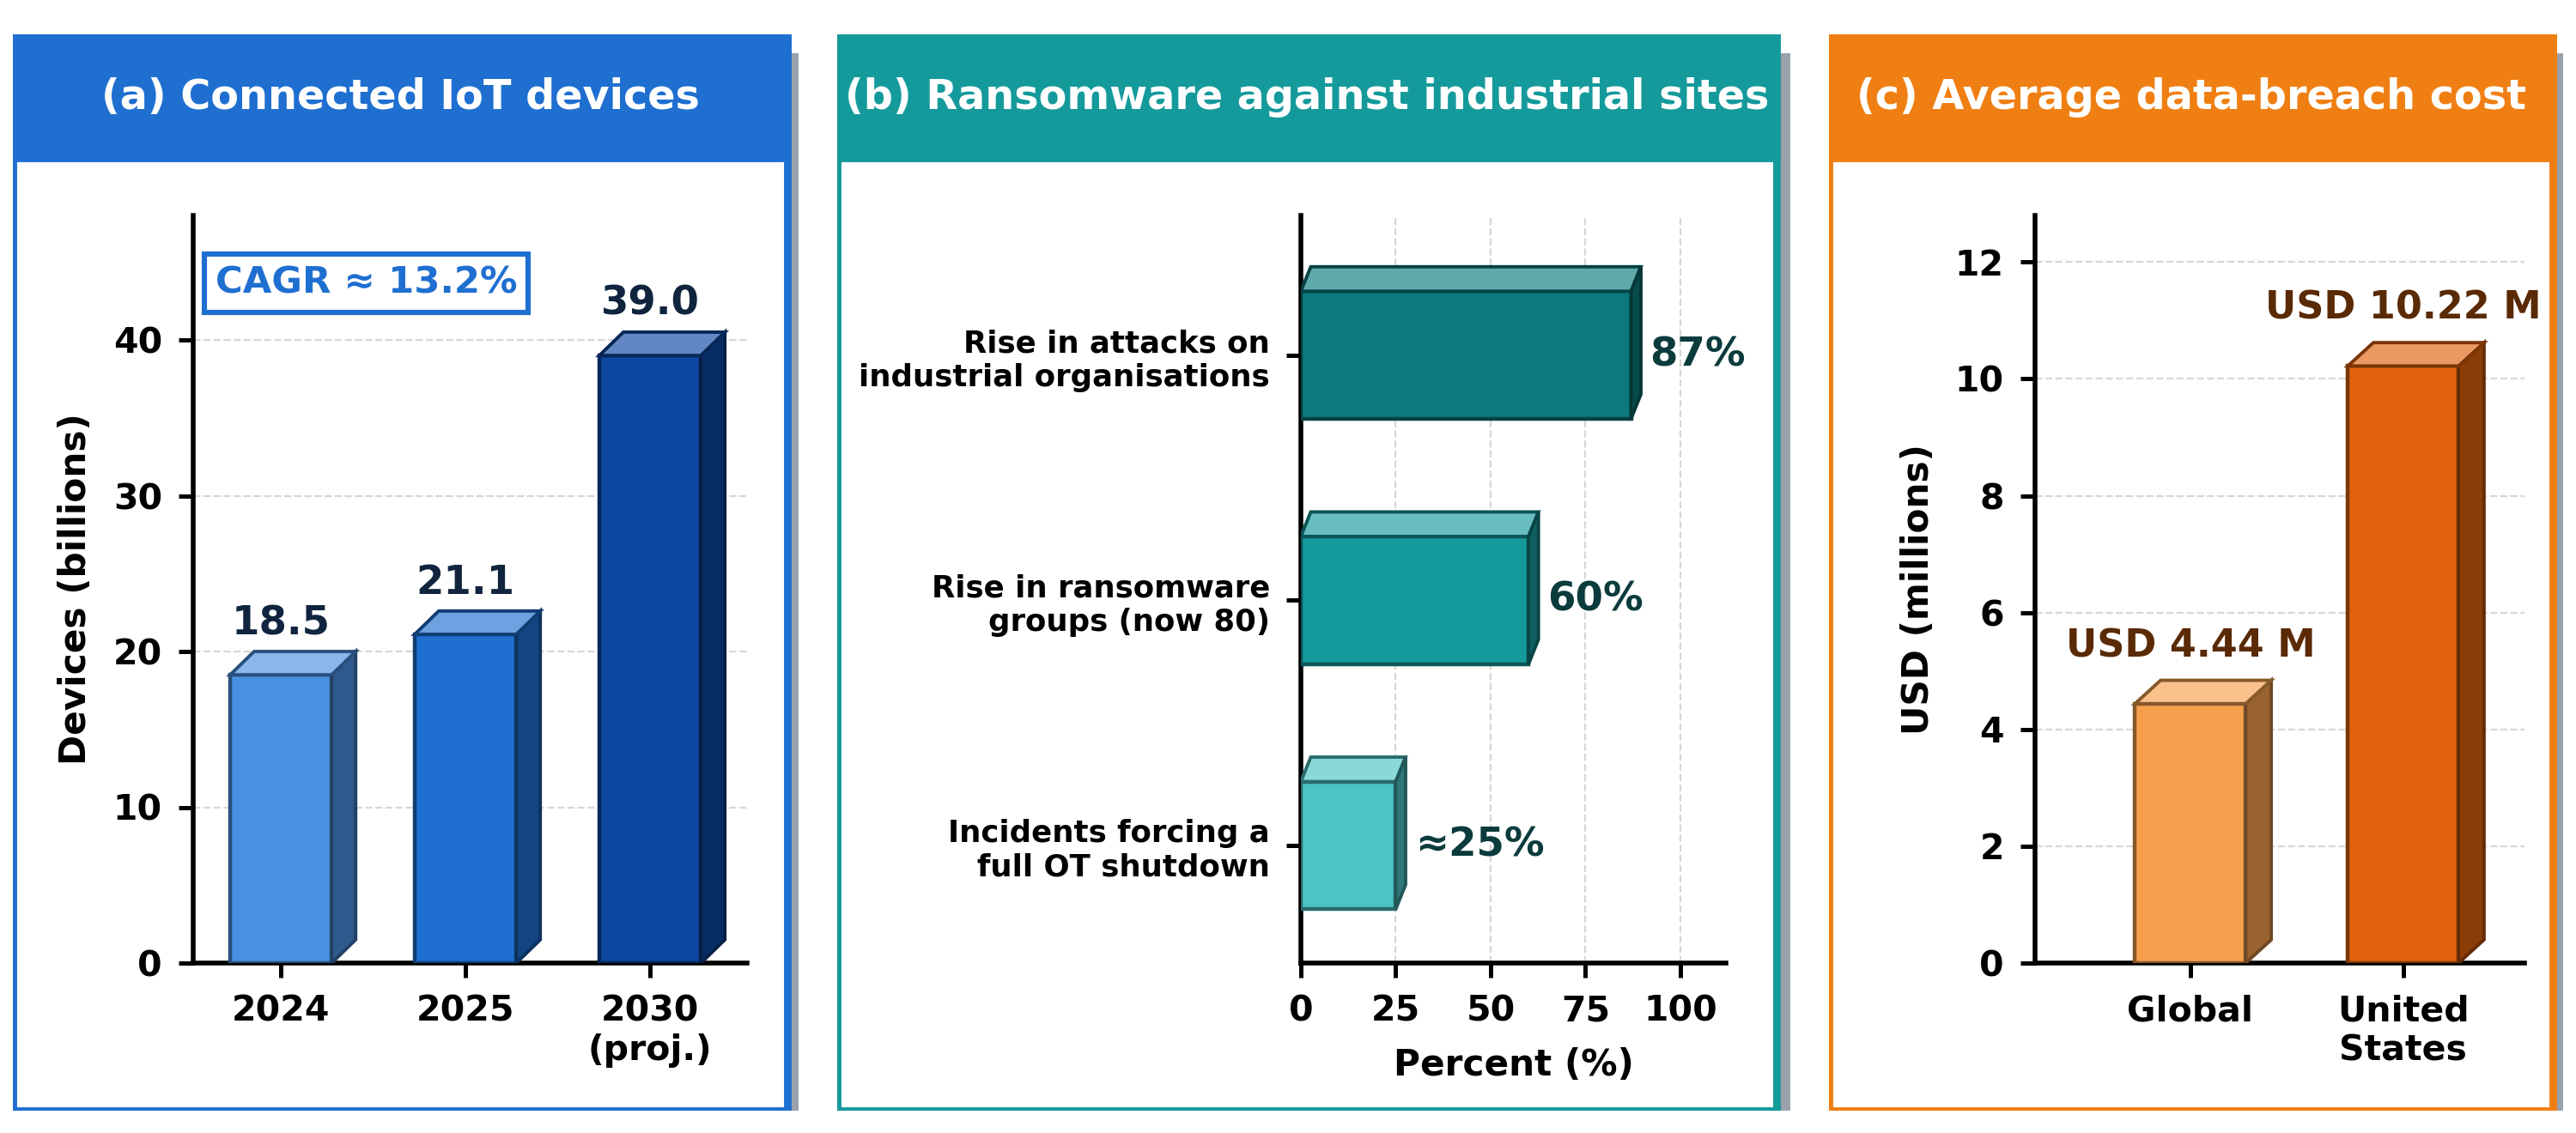
\includegraphics[width=\textwidth]{figures/Fig1_2_landscape.png}
    \caption{Indicators of the IIoT security landscape: (a) growth of connected IoT devices from 2024 to 2030~\cite{iotanalytics2025}; (b) ransomware activity against industrial organisations~\cite{dragos2025}; and (c) the average cost of a data breach globally and in the United States~\cite{ibm2025}.}
    \label{fig:landscape}
\end{figure}
 
The nodes at the edge of an IIoT deployment are severely resource-constrained,
operating within tight budgets of computation, memory, and energy. These
constraints hinder the deployment of conventional deep learning-based intrusion
detection and heavyweight cryptographic machinery on the very devices that most
require protection~\cite{amadi2026lightweight}. The central engineering tension of
secure IIoT is therefore not whether strong protection exists, but whether it
can be delivered within the resource envelope of constrained devices without
sacrificing the real-time responsiveness that mission-critical operations
demand.
 
Distributed ledgers are a natural foundation for tamper-evident trust among such
devices, yet they bring a constraint of their own. This tension is a concrete
instance of the well-documented blockchain trilemma: the difficulty of
simultaneously achieving security, scalability, and speed
within a single distributed-ledger system, where optimising any two dimensions
tends to come at the expense of the third~\cite{aiv_own}. Recent theoretical
work argues that these trade-offs are not merely engineering compromises but
reflect fundamental limits, supported by formal proofs of their
inevitability~\cite{nakai, mssassi, monte}. In safety-critical,
resource-constrained settings the trilemma is at its most acute, since none of
the three dimensions can be relaxed without unacceptable consequence.
 
A further pressure compounds the problem. The asymmetric cryptography that
underpins current authentication and key exchange, namely RSA and
elliptic-curve schemes, is vulnerable to a sufficiently capable quantum computer executing
Shor's algorithm~\cite{shor1999polynomial}. The risk is not deferred to the
arrival of such a machine: under the ``harvest-now, decrypt-later'' model, an
adversary can capture encrypted traffic today and decrypt it retroactively once
the capability matures, placing data with long confidentiality horizons at
present risk~\cite{kagai2025harvest}. This
concern is now codified rather than speculative. In August 2024, the U.S.
National Institute of Standards and Technology finalised its first
post-quantum cryptographic standards, FIPS~203 (ML-KEM, derived from
CRYSTALS-Kyber), FIPS~204 (ML-DSA), and FIPS~205 (SLH-DSA), concluding a
standardisation process initiated in 2016~\cite{fips203, fips204, fips205}. For
constrained IIoT the challenge is sharper still, as post-quantum primitives
carry larger keys and ciphertexts than the schemes they replace and must be made
to fit hardware already strained by classical cryptography.

\begin{figure}[htbp]
    \centering
    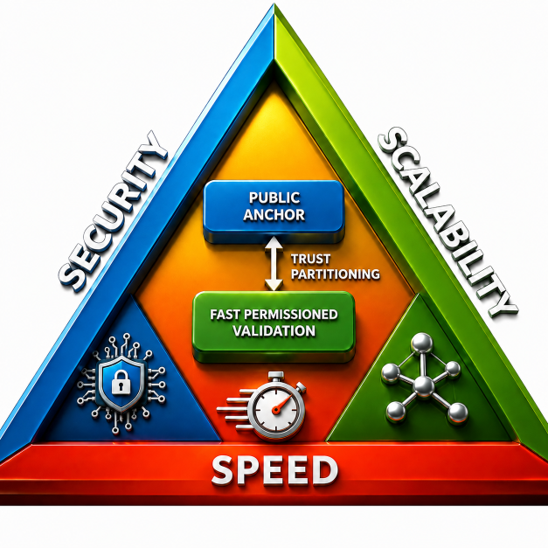
\includegraphics[width=0.70\textwidth]{figures/Picture1.png}
    \caption{The security, scalability, and speed trilemma in constrained mission-critical IIoT, and the trust-partitioning response adopted in this thesis, in which fast permissioned validation is separated from public anchoring.}
    \label{trilemma}
\end{figure}

Several approaches have been proposed to meet these pressures, but each resolves
one at the expense of another. Learning-based detectors built on convolutional,
recurrent, and hybrid convolutional-recurrent models achieve strong accuracy on
industrial traffic~\cite{chen2025cnnlstm, anwer2025federated}, and federated
variants keep raw data on the premises that generate
it~\cite{lee2025lightweight, mao2025fedinnid}. However, the trust verdict these
detectors produce is stored wherever the model runs, so it remains as mutable as
its host. Permissioned ledgers coupled to intrusion detection make such verdicts
tamper-evident~\cite{song2025hybrid, peng2025bctdics}, yet committing at
industrial event rates strains consensus throughput and on-chain
storage~\cite{xiong2025sharding, ding2025dcstorage}. Hybrid and tiered ledgers
reconcile operational speed with external verifiability by anchoring a compact
digest of a fast permissioned layer on a public
chain~\cite{ullah2025mbid, banitalebi2025edblsd}. In doing so, however, they make
the cross-chain link the weakest point of the combined
system~\cite{zhou2025bridgeguard}, and the quantum-resistant primitives needed
to keep the anchored record durable carry keys and signatures that collide with
the budgets of constrained devices~\cite{hanna2025comprehensive, cruz2025measuring}.
What is required is therefore not a stronger single layer of protection, but a
design that places each security function where its cost can be sustained.
 
Taken together, these forces define the gap this thesis addresses. Trustworthy
IIoT security must be affordable within real device resource budgets, responsive
enough for mission-critical operation, scalable across large deployments, and
resilient against an emerging quantum adversary, a combination that a single,
uniform security layer cannot satisfy simultaneously. The position advanced in this thesis is that these demands become jointly achievable when trust is not
applied uniformly but is partitioned across a tiered architecture:
high-frequency behavioural validation is routed through a fast, permissioned
layer close to the devices, while low-frequency, high-value events such as
identity anchoring, audit, and revocation are committed to a separate public
layer, as illustrated in Fig.~\ref{trilemma}. Routing sensitive,
high-frequency interactions through permissioned consensus while anchoring
integrity proofs and audit trails on public chains has been argued to be a
structural necessity rather than a mere performance optimisation for demanding
data-sharing environments~\cite{amadi2026security}. This principle of trust-partitioning across a hybrid
ledger, and its realisation within real device budgets and across distinct
ledger substrates, forms the central contribution of this thesis.


\section{Motivation for Research}
\label{motivation}

This study is motivated by the gap between the security that mission-critical
IIoT requires and the security that constrained industrial hardware can afford.
Existing approaches tend to optimise one dimension at the expense of the others.
Many intrusion-detection methods pursue model accuracy without demonstrating
that the model, together with its supporting ledger, can run on a low-power node;
many blockchain provenance schemes secure storage without establishing
feasibility on constrained devices; and most report neither a complete
evaluation across both the artificial-intelligence and blockchain layers nor the
blockchain-side costs, such as gas consumption, transaction latency, and
smart-contract security, that determine real-world viability. At the same time,
the reliance on classical asymmetric cryptography leaves long-lived industrial
data exposed to a quantum adversary under the harvest-now, decrypt-later model,
a concern now formalised by the standardisation of post-quantum algorithms.
Rather than treating efficiency, security, and quantum resilience as competing
objectives to be traded against one another, this research is driven by the view
that they can be reconciled by disaggregating trust across a tiered architecture,
so that each security function is placed on the layer whose cost profile it can
sustain. The aim is a security design that is lightweight, verifiable, and
deployable on real industrial devices, and whose organising principle
generalises beyond any single implementation.

\section{Research Breakdown and Major Contributions}
\label{sec:rq}

The foregoing analysis exposes a single overarching problem. How can trustworthy
security be delivered for constrained, mission-critical IIoT when the devices
that carry the security burden cannot afford uniform, heavyweight protection,
and when the underlying cryptography faces an emerging quantum threat? From this
problem, the following research questions follow:

\begin{enumerate}
  \item \textbf{Trust partitioning:} Can trust be partitioned across a hybrid
        ledger, so that high-frequency behavioural validation is handled on a
        fast permissioned layer while low-frequency, high-value events such as
        identity anchoring, audit, and revocation are committed to a separate
        anchoring layer, and does this partitioning deliver trustworthy security
        within real device resource budgets?

  \item \textbf{Lightweight behavioural trust:} Can lightweight
        artificial-intelligence behavioural trust scoring operate inside the
        compute, memory, and energy budgets of real constrained IIoT devices
        without sacrificing detection performance?

  \item \textbf{Quantum-resilient identity:} Can post-quantum-resilient identity
        and credential delivery be achieved on such hardware without prohibitive
        latency or bandwidth cost?

  \item \textbf{Substrate independence:} Does the trust-partitioning principle
        hold across distinct ledger substrates, rather than being an artefact of
        a single implementation?

  \item \textbf{Adversarial robustness:} Under adversarial conditions, can
        behavioural trust scoring with decay-based revocation reliably isolate a
        misbehaving node while the hybrid-ledger architecture sustains
        dependable detection performance?
\end{enumerate}

Answering these questions requires an architecture that reconciles scalability
with speed and security while carrying out validation and anchoring within the
resource limits of industrial edge hardware. The goal of this thesis is
therefore to establish that trustworthy security for constrained,
mission-critical IIoT is achievable by partitioning trust across a hybrid-ledger
architecture, in which high-frequency behavioural validation is handled on a
fast permissioned layer and low-frequency, high-value events are anchored on a
public layer, and to demonstrate this within real device resource budgets and
across more than one ledger substrate. Toward this goal, this research makes the
following contributions:

\begin{enumerate}
  \item It introduces STRATA, a unified trust-partitioning architecture for
        constrained, mission-critical IIoT, in which high-frequency behavioural
        validation on a fast permissioned layer is separated from low-frequency
        identity anchoring and audit committed to a public layer, and it
        consolidates three published
        systems~\cite{amadi2026lightweight, amadi2025quantum, amadi2026symmetric}
        as instances of this single architecture rather than as independent
        designs.

  \item It presents a lightweight federated behavioural-trust module built on a
        trimmed one-dimensional CNN-LSTM model coupled with a resource-optimised
        permissioned ledger, and evaluates it end to end across both the
        artificial-intelligence and blockchain layers, reporting detection
        performance together with blockchain-side
        costs~\cite{amadi2026lightweight}.

  \item It presents a quantum-resilient identity and credential module based on
        entropy-seeded identity generation and compressed post-quantum key
        delivery, and demonstrates its feasibility on constrained hardware,
        distinguishing clearly between the components that are implemented and
        measured and those reserved as design~\cite{amadi2025quantum}.

  \item It demonstrates that the trust-partitioning principle is
        substrate-independent by realising it on two distinct ledger
        substrates~\cite{amadi2026lightweight, amadi2026symmetric}, and it provides a consolidated evaluation, spanning
        detection performance, resource overhead, blockchain cost, and
        quantum-resilience, that assesses the architecture against the resource
        constraints of industrial edge devices.
\end{enumerate}

The systematic review in Chapter~3 found no prior work that establishes trust
partitioning across a hybrid ledger as a unifying principle for constrained,
mission-critical IIoT, demonstrated within real device budgets and shown to hold
across distinct ledger substrates. This constitutes the novelty of the thesis.

Table~\ref{tab:rq-map} maps each research question to the contribution that
answers it, the sections in which it is designed and evaluated, and the
published work on which it builds.
\begin{table}[htbp]
\centering
\footnotesize
\setlength{\tabcolsep}{4pt}
\renewcommand{\arraystretch}{1.35}
\caption{Mapping of the research questions to the contributions, the thesis sections that design and evaluate them, and the underlying publications.}
\label{tab:rq-map}
\begin{tabularx}{\textwidth}{@{}
    >{\raggedright\arraybackslash}p{0.9cm}
    >{\raggedright\arraybackslash}X
    >{\centering\arraybackslash}p{1.3cm}
    >{\raggedright\arraybackslash}p{2.1cm}
    >{\raggedright\arraybackslash}p{2.4cm}
    >{\raggedright\arraybackslash}p{2.2cm}@{}}
\toprule
\textbf{RQ} & \textbf{Focus} & \textbf{Contri\-bution} & \textbf{Design (Ch.~4)} & \textbf{Evaluation (Ch.~5)} & \textbf{Publication} \\
\midrule
RQ1 & Partitioning trust across a hybrid ledger within device budgets
    & 1 & \ref{sec:strata-principle}, \ref{sec:strata-anchor}
    & \ref{sec:eval-ledger}, \ref{sec:eval-trilemma}
    & \cite{amadi2026security, amadi2026lightweight} \\
RQ2 & Lightweight behavioural trust scoring on constrained devices
    & 2 & \ref{sec:strata-trust}
    & \ref{sec:eval-evidence}, \ref{sec:eval-learning}, \ref{sec:eval-resource}
    & \cite{amadi2026lightweight} \\
RQ3 & Quantum-resilient identity and credential delivery
    & 3 & \ref{sec:plane-b}
    & \ref{sec:eval-identity}
    & \cite{amadi2025quantum, amadi2026symmetric} \\
RQ4 & Substrate independence of trust partitioning
    & 4 & \ref{sec:strata-substrates}
    & \ref{sec:eval-substrate}
    & \cite{amadi2026lightweight, amadi2026symmetric} \\
RQ5 & Isolating a misbehaving node under adversarial conditions
    & 2, 3 & \ref{sec:plane-a}
    & \ref{sec:eval-security}, \ref{sec:eval-isolation}
    & \cite{amadi2026symmetric} \\
\bottomrule
\multicolumn{6}{@{}p{\textwidth}@{}}{\scriptsize The trilemma framing of Chapters~1 and~2 draws on~\cite{aiv_own}, and the systematic review of Chapter~3 extends~\cite{amadi2026security}.}
\end{tabularx}
\end{table}

\label{sec:organisation}
The organisation of this thesis is as follows. Chapter~\ref{Chapter_1}
presents the introduction, the motivation, the research questions, and the
contributions. Chapter~2 provides the background, covering consensus and hybrid
ledgers, post-quantum cryptography, and lightweight learning for anomaly
detection. Chapter~3 reviews related work and, through a systematic analysis,
identifies the defence gap that the thesis addresses. Chapter~4 presents the
STRATA architecture and its constituent modules as instances of a single
trust-partitioning design. Chapter~5 reports the consolidated evaluation across
detection performance, resource overhead, blockchain cost, and quantum
resilience. The thesis is concluded in Chapter~6 with a summary of
contributions, the disclosed limitations, and directions for future work.
Fig.~\ref{fig:roadmap} presents this structure as a roadmap, indicating the
research questions each chapter addresses.

\begin{figure}[htbp]
    \centering
    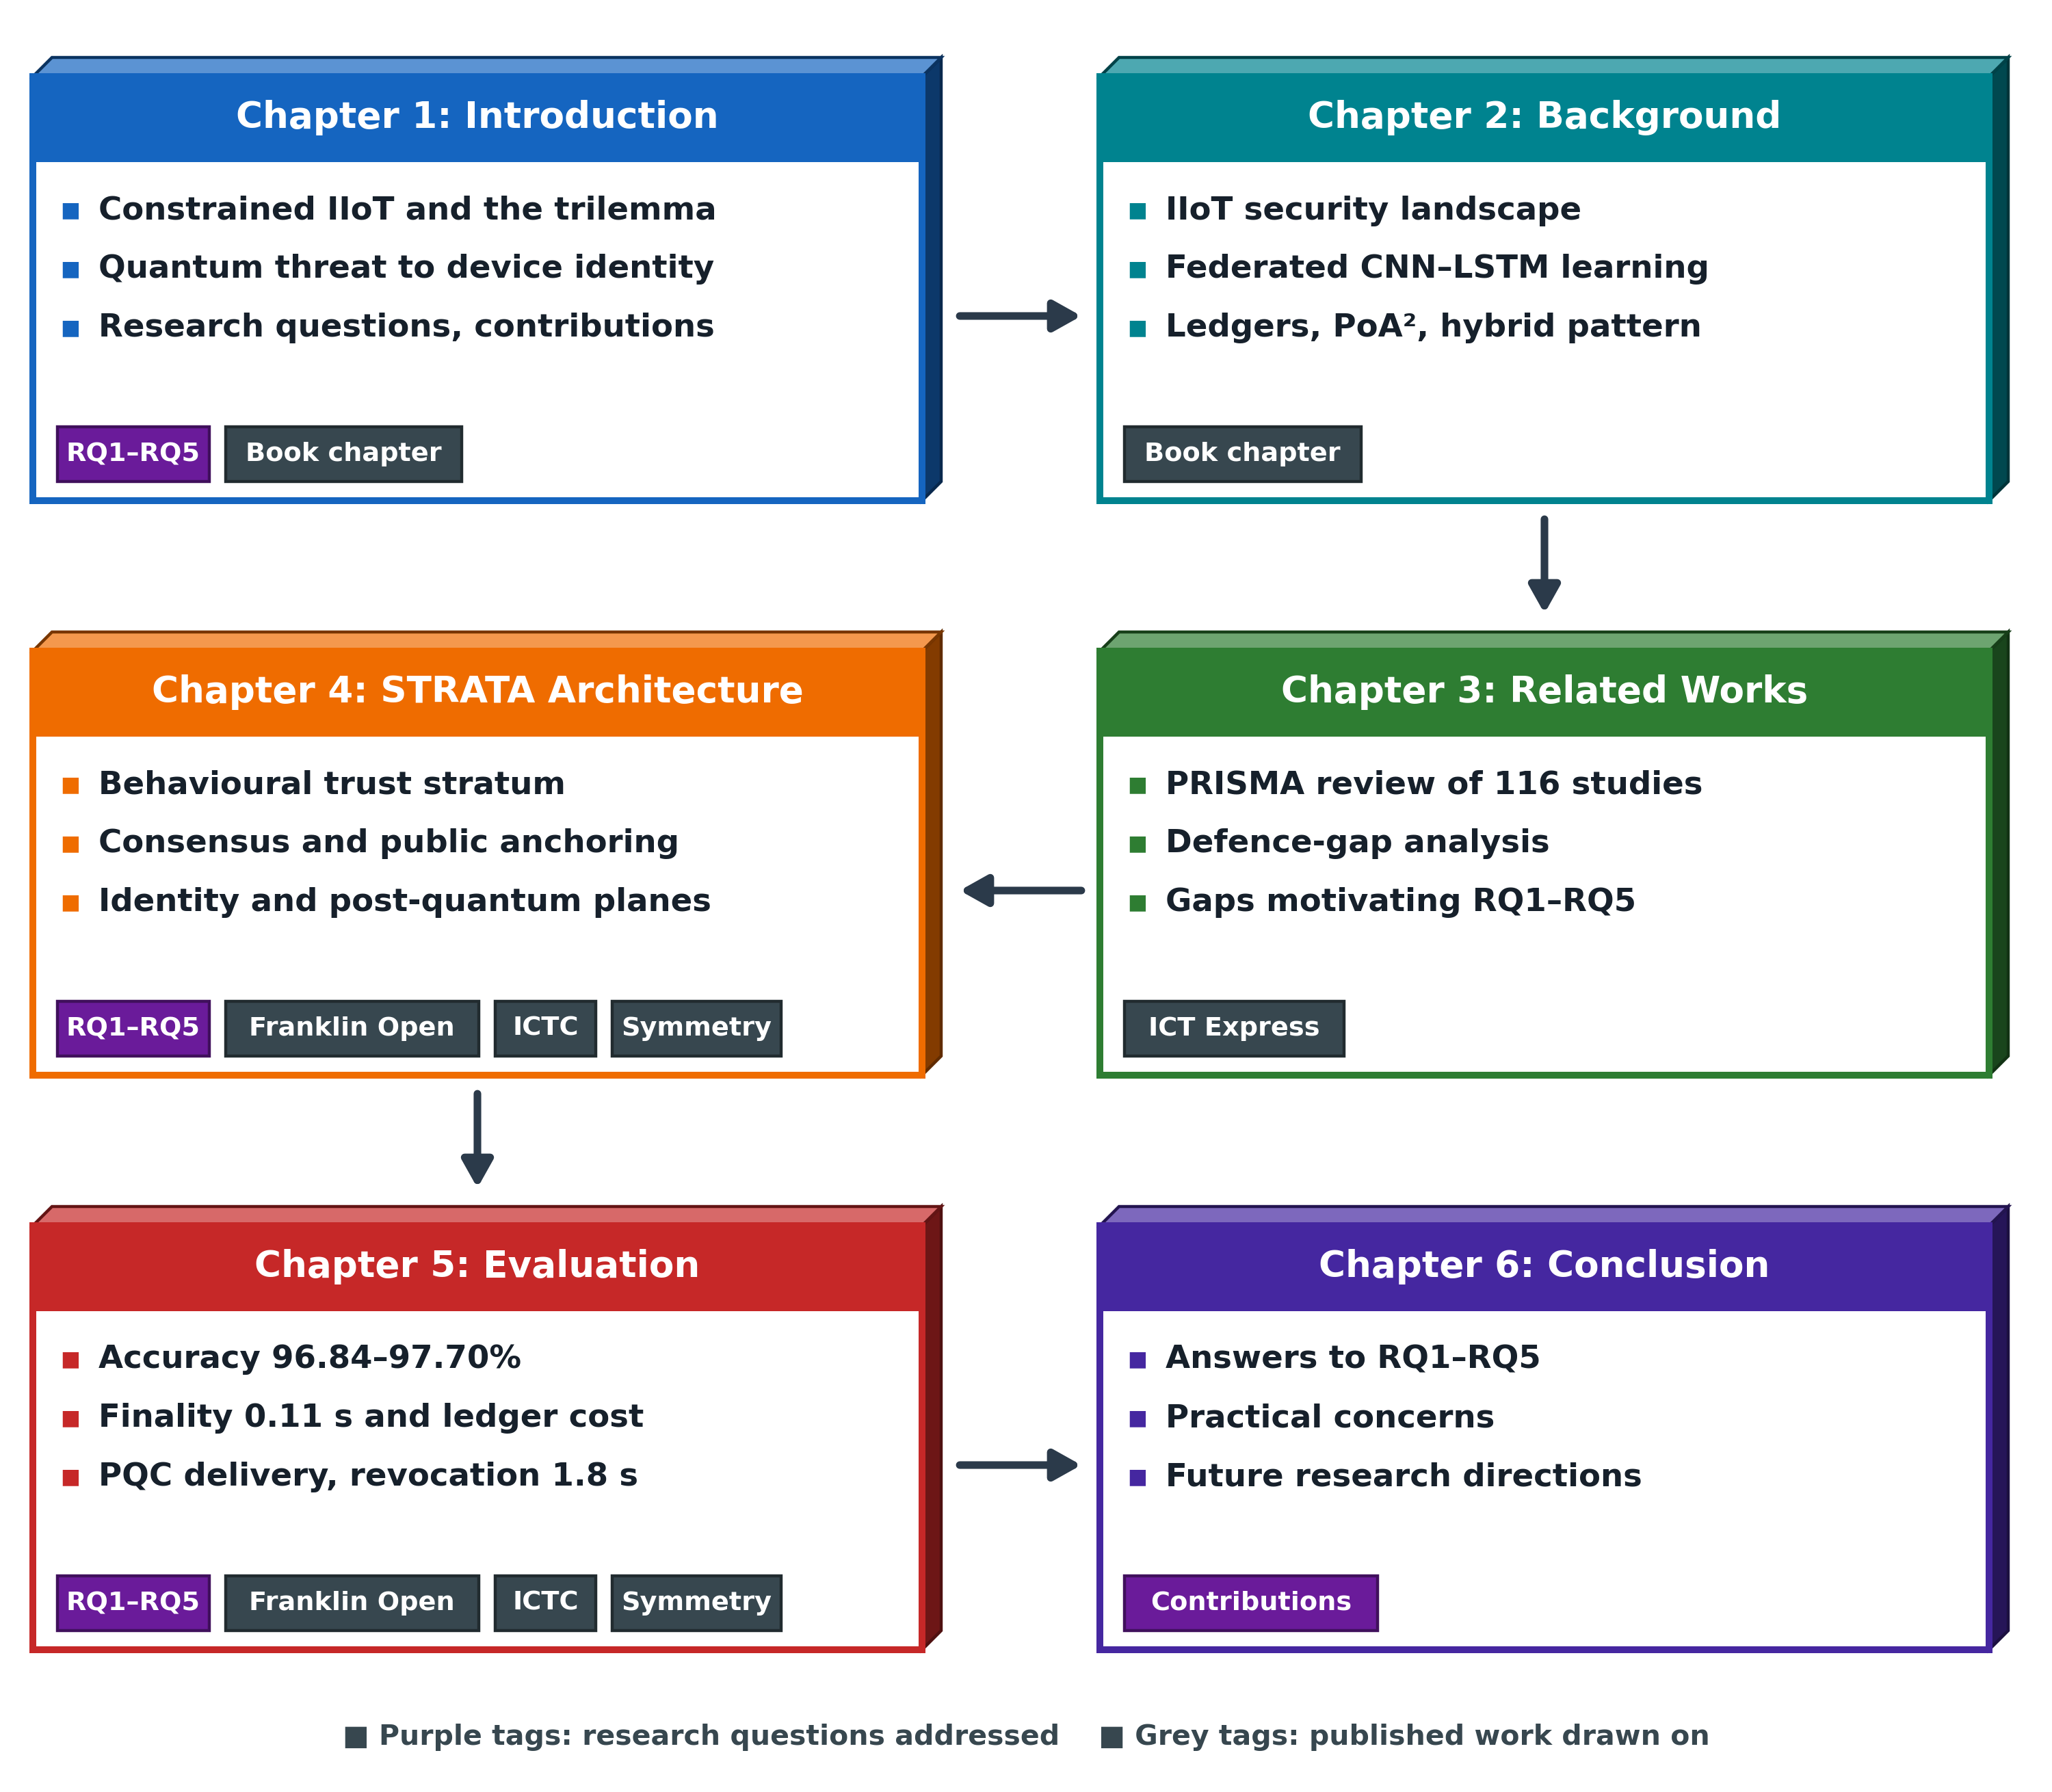
\includegraphics[width=\textwidth]{figures/Fig1_3_roadmap.png}
    \caption{Roadmap of the thesis, showing the flow from problem definition to the STRATA architecture, its evaluation, and the conclusions, together with the research questions associated with each chapter.}
    \label{fig:roadmap}
\end{figure}


\chapter{Background Information}
% \pagenumbering{arabic}
\Large
% \normalsize
\label{Chapter_2}
\section{Industrial IoT Security Landscape}
\label{sec:bg-landscape}

This section establishes the terrain on which this work is built. It defines the
Industrial Internet of Things and its mission-critical role, traces the evolution
that has led from isolated industrial control systems to the partitioned,
quantum-aware trust architectures examined here, characterises the scale of
deployment and the threat landscape it invites,  and reviews the regulatory
and standards context within which any deployable system must sit.
 
\subsection{From Industrial Control Systems to Trust-Partitioned IIoT}
\label{subsec:bg-evolution}
 
Industrial computing has passed through several distinct eras, and the security
problem addressed here is a product of that progression. Early industrial
control systems were isolated: programmable logic controllers and supervisory
systems operated on air-gapped networks, and security rested largely on physical
separation rather than on cryptography \cite{hussain2025survey}. The Industrial Internet of Things
dissolved that separation\cite{enemosah2024scada, kebande2024industrial}. By interconnecting sensors, controllers, actuators,
and gateways over shared networks, IIoT delivered real-time monitoring and
adaptive control, but it also exposed formerly isolated equipment to remote
adversaries\cite{kayan2022cybersecurity,zhukabayeva2025cybersecurity}. Subsequent phases layered artificial intelligence onto this fabric
for behavioural anomaly detection \cite{pinto2023survey, nuaimi2023intelligent}, and then introduced blockchain to provide
tamper-evident provenance for the data and decisions that AI produced \cite{amadi2026security,khan2022internet,huo2022comprehensive}. The
present phase, the one STRATA occupies, adds two further requirements: that trust
be partitioned across tiered ledgers so that heavyweight security work does not
fall on the weakest devices, and that the cryptography underpinning identity and
key exchange be resilient against an emerging quantum adversary.
Figure~\ref{fig:iiot-evolution} traces this progression and situates the present
contribution at its endpoint.


\begin{figure}[htbp]
    \centering
     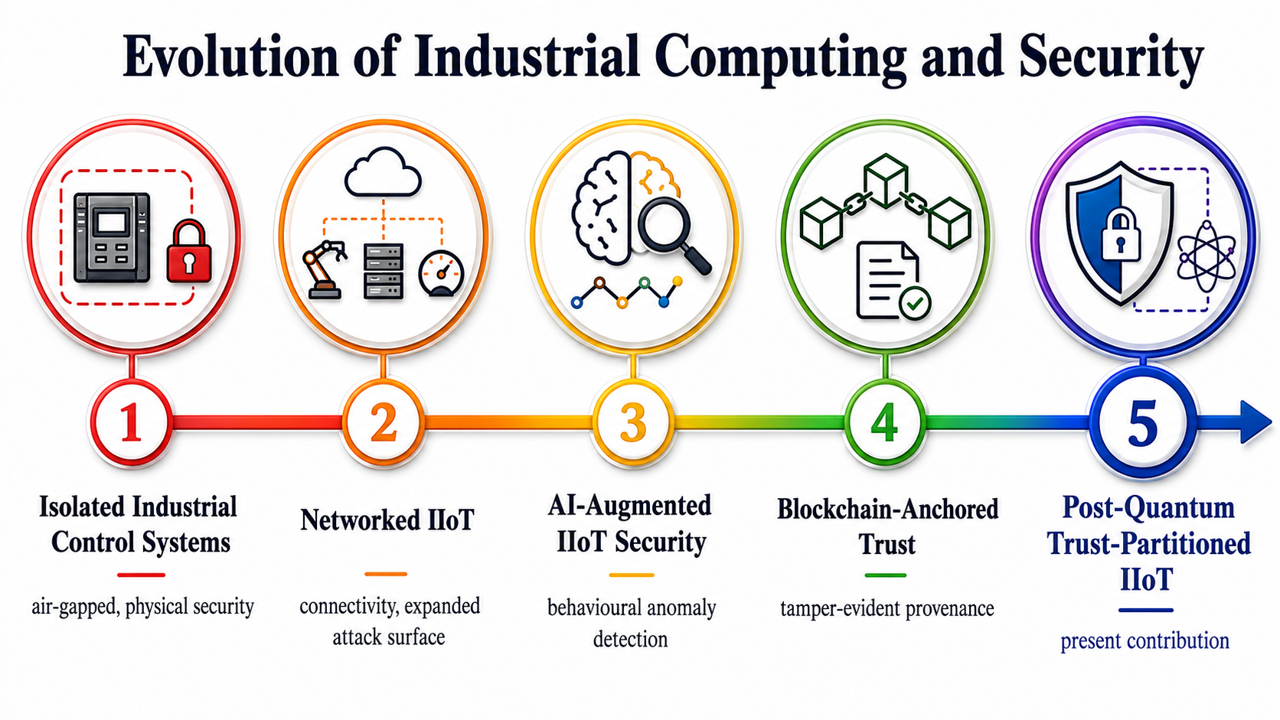
\includegraphics[width=0.95\textwidth]{figures/Picture2-evolution.png}
    \caption{Evolution of industrial computing security, from isolated control
    systems to post-quantum, trust-partitioned architecture.}
    \label{fig:iiot-evolution}
\end{figure}
 
\subsection{Scale and Mission-Critical Role}
\label{subsec:bg-scale}
 
The IIoT is now infrastructure at a scale that makes its security a matter of
public consequence rather than private inconvenience. The global installed base
of connected IoT devices reached approximately 18.5~billion in 2024 and is
projected to grow to 21.1~billion by the end of 2025 and to 39~billion by 2030,
a compound annual growth rate of about 13.2\%~\cite{iotanalytics2025}. The data
these devices generate grows in step with their number: IDC's Data Age 2025
study forecast that the global datasphere, the total volume of data created,
captured, and replicated worldwide each year, would expand from 45~zettabytes in
2019 to 175~zettabytes by 2025~\cite{idc_dataage2025}. A growing share of this
base is embedded in manufacturing, energy, water, and transportation systems,
where the data exchanged does not merely inform but directly actuates physical
processes. In such settings a corrupted reading, a forged command, or a delayed
validation is not a data-quality issue but a safety and continuity issue\cite{yu2023survey}, and
this is what distinguishes industrial security from its enterprise counterpart\cite{lehto2022cyber}.
Table~\ref{tab:iiot-stats} consolidates the scale, threat, and cost figures that
frame the problem, each drawn from its primary source.
 


\begin{table}[htbp]
\centering
\caption{Quantitative indicators motivating IIoT security: scale of deployment,
rise in attacks, cost of breaches, and cryptographic urgency.}
\label{tab:iiot-stats}
\small
\renewcommand{\arraystretch}{1.4}
\arrayrulecolor{red!70!black}
\begin{tabular}{@{}l r p{6.2cm}@{}}
\specialrule{1.2pt}{0pt}{0pt}
\rowcolor{red!12}
\textbf{Dimension} & \textbf{Quantity} & \textbf{Interpretation} \\
\specialrule{1.2pt}{0pt}{0pt}
\arrayrulecolor{black}
\textbf{Scale}
  & 18.5 $\rightarrow$ 39 billion
  & Connected IoT devices, 2024 to 2030 (projected), a 13.2\% compound annual growth rate. \\
\addlinespace
  & 175 ZB
  & Global data volume forecast for 2025. \\
\midrule
\textbf{Threat}
  & $+87\%$
  & Year-over-year rise in ransomware against industrial systems. \\
\addlinespace
  & $>50\%$
  & Share of ransomware victims in manufacturing. \\
\addlinespace
  & 25\%
  & Incidents forcing a full operational-technology shutdown. \\
\midrule
\textbf{Cost}
  & USD 4.44 M
  & Average cost of a data breach, global. \\
\addlinespace
  & USD 10.22 M
  & Average cost of a data breach, United States. \\
\midrule
\textbf{Urgency}
  & 2024
  & Post-quantum standards (FIPS 203/204/205) finalised, starting migration deadlines for current cryptography. \\
\arrayrulecolor{red!70!black}
\specialrule{1.2pt}{0pt}{0pt}
\arrayrulecolor{black}
\end{tabular}

\vspace{4pt}
{\footnotesize\itshape Sources: IoT Analytics (2025); IDC Data Age 2025;
Dragos (2025); IBM/Ponemon (2025); NIST (2024).}
\end{table}
 
\subsection{The Threat Landscape}
\label{subsec:bg-threats}
The consequence of pervasive connectivity is a substantially enlarged attack surface. Operational-technology environments, once peripheral to attacker interest, have become primary targets. Ransomware activity against industrial
organisations rose by more than 87\% year over year, the number of ransomware
groups directing effort at such organisations grew by 60\% to reach 80, and
manufacturing alone accounted for more than half of observed victims, with
roughly a quarter of incidents forcing a full shutdown of the affected
site~\cite{dragos2025}. The financial weight is of comparable order, the global
average cost of a data breach reaching USD~4.44~million and rising to
USD~10.22~million in the United States~\cite{ibm2025}. Beyond their headline
magnitude, these figures matter because industrial incidents convert directly
into physical disruption, which raises the stakes of every security decision at
the device level~\cite{yu2023survey}.

The specific forms these attacks take on industrial networks can be organised by
their traffic-level behaviour~\cite{aslam2024scrutinizing, sasi2024comprehensive}.
Denial-of-service and distributed denial-of-service attacks manifest as high-rate
flooding that saturates controllers and gateways; reconnaissance appears as
systematic probing of control-protocol ports; credential attacks show as
repeated authentication failures against brokers and controller interfaces; and
infiltration and botnet activity appear as anomalous payload entropy and periodic beaconing~\cite{gelgi2024systematic}. Table~\ref{tab:attack-map} maps these categories to their industrial manifestations, following the characterisation used in the behavioural detection work of Chapter~\ref{Chapter_4}.

\begin{table}[htbp]
\centering
\caption{Common attack categories and their manifestation in industrial network
traffic.}
\label{tab:attack-map}
\small
\begin{tabular}{p{3.0cm} p{4.5cm} p{5.0cm}}
\toprule
\textbf{Attack category} & \textbf{Traffic-level behaviour} & \textbf{Industrial manifestation} \\
\midrule
DoS / DDoS & High-rate flooding above normal baseline & Controller or gateway saturation, sensor jamming \\
Port scanning & Aggressive probing of many ports & Enumeration of control-protocol ports before intrusion \\
Brute force & Repeated authentication failures & Credential guessing against brokers and controller logins \\
Infiltration / malware & Elevated payload entropy, irregular flow sizes & Unauthorised firmware upload, code injection \\
Botnet / command-and-control & Periodic beaconing, low-entropy commands & Compromised devices in coordinated attacks \\
\bottomrule
\end{tabular}
\end{table}
 

\begin{figure}[htbp]
    \centering
     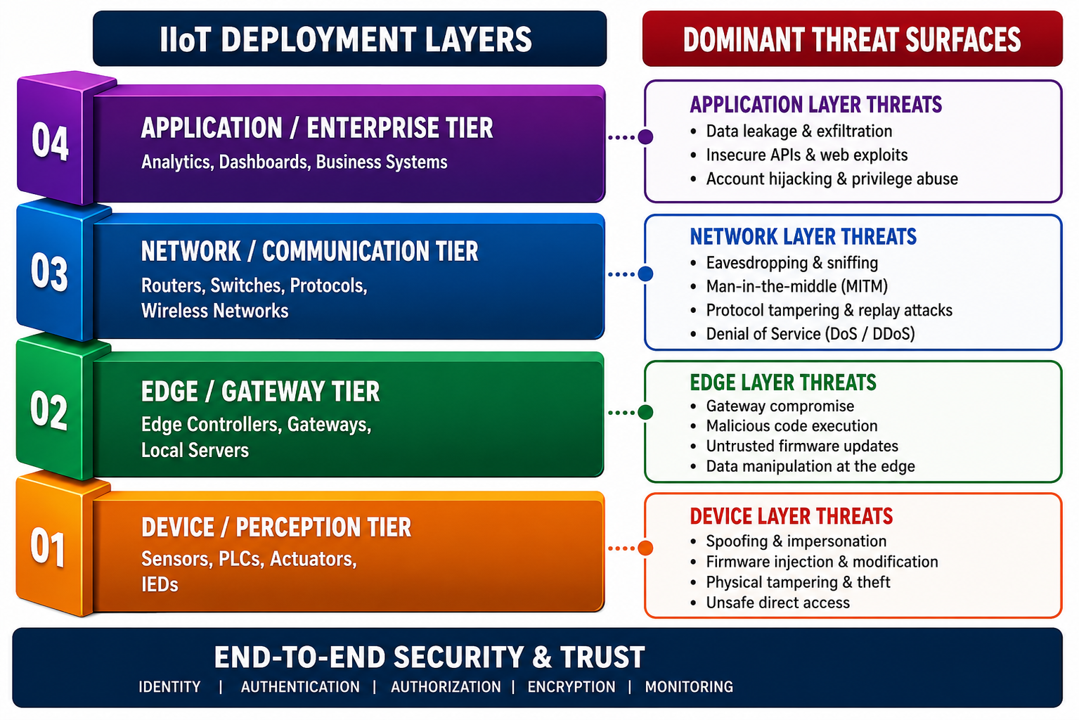
\includegraphics[width=0.95\textwidth]{figures/Picture3_threat.png}
    \caption{Layered view of an industrial IoT deployment and the dominant threat surface at each tier.}
    \label{fig:iiot-stack}
\end{figure}
 
\subsection{Regulatory and Standards Context}
\label{subsec:bg-regulatory}
Any deployable industrial security system sits within a regulatory and standards
environment that is itself evolving. The strategic value of industrial data
sharing is increasingly recognised in policy, with instruments such as the EU
Data Act of 2023 reflecting formal recognition of its
importance~\cite{stripped}. % TODO: replace `stripped` with the real EU Data Act entry from your DT paper's .bib

The cryptographic side of this environment has shifted even more sharply. The
asymmetric schemes that underpin current authentication and key exchange derive
their security from problems that a sufficiently capable quantum computer could
solve efficiently using Shor's algorithm~\cite{shor1999polynomial}. The risk is
not deferred to the arrival of such a machine: under the harvest-now,
decrypt-later model, an adversary can capture encrypted traffic today and decrypt
it once the capability matures, placing data with a long confidentiality horizon
at present risk~\cite{kagai2025harvest}. These pressures moved the quantum threat
from a research concern to a compliance one. In August 2024 the United States
National Institute of Standards and Technology finalised its first post-quantum
standards, FIPS 203, FIPS 204, and FIPS 205, concluding a process begun in
2016~\cite{fips203, fips204, fips205}.

The practical consequence for industrial deployment is that migration toward
quantum-resilient primitives is now an anticipated requirement rather than an
optional enhancement, and systems designed today are reasonably expected to
accommodate it~\cite{wang2025review}. The tension this creates for constrained
hardware, namely that post-quantum primitives carry larger keys and ciphertexts
than the schemes they replace and must be made to fit devices that are already
limited, is one of the motivating problems addressed in the chapters that
follow~\cite{fitzgibbon2024constrained}.



% ============================================================
% Chapter 2 — Section 2.2 (rich build)
% Learning-Based Security for Constrained IIoT
% Style: no em-dashes, no \emph, direct register (no "this thesis"/"we").
% Scope: MECHANISMS only. No measured results (params, accuracy, latency
% belong in Ch.4/5). Does NOT re-argue the constrained-hardware limits
% already covered in 2.1.4; here the focus is the learning methods.
%
% CITATION FLAGS: each [CITE: ...] marks a spot needing an external
% scholarly source, with a suggested Scholar search. Your own papers are
% cited with placeholder keys (amadi2026lightweight / amadi2026security /
% amadi2026identity) — confirm these match your .bib.
% ============================================================

\section{Learning-Based Security for Constrained IIoT}
\label{sec:bg-learning}

Signature-based and rule-based defences, which match traffic against catalogues
of known attack patterns, are poorly suited to industrial IoT. They cannot
recognise novel or zero-day behaviour, they require constant manual updating, and
their central deployment assumes a visibility over device traffic that
distributed industrial networks do not provide. Learning-based methods address
these gaps by modelling normal behaviour and flagging deviations from it, which
allows previously unseen attacks to be detected as anomalies rather than as known
signatures. This section explains the learning methods on which the systems in
this work rest: federated learning as the training paradigm, a hybrid
convolutional and recurrent network as the detection engine, and threshold-based
trust scoring as the mechanism that converts a detection into an enforceable
decision. The concern throughout is with how these methods operate; their
measured behaviour is reported in the evaluation.

\subsection{Federated Learning}
\label{subsec:bg-fl}

Conventional machine-learning pipelines are centralised: data is gathered from its
sources into a single repository where a model is trained. In distributed
industrial settings this arrangement is problematic on two counts. Transmitting
raw operational data to a central server consumes bandwidth that constrained
networks cannot spare, and it exposes sensitive process data to interception and
to privacy or confidentiality concerns\cite{lu2024federated,dritsas2025federated}.

Federated learning removes the need to centralise raw data. Each participating
device trains a local copy of a shared model on its own data and transmits only
the resulting model update, the adjusted parameters, to a coordinating
aggregator. The aggregator combines the updates from all participants into an
improved global model and returns it for the next round of local training. The
canonical aggregation rule, federated averaging, computes the global model as a
weighted average of the client updates, with each client weighted by the size of
its local dataset so that participants holding more data contribute
proportionally~\cite{amadi2026lightweight}. Because the raw data never leaves the
device on which it was generated, federated learning reduces both the
communication cost and the privacy exposure of collaborative training, which is
what makes it appropriate for distributed industrial deployments in which data is
sensitive and connectivity is limited\cite{ali2024blockchain}. Table~\ref{tab:central-vs-fl} contrasts the
two training paradigms across the dimensions that matter for constrained
industrial deployment.

\begin{table}[htbp]
\centering
\caption{Centralised and federated learning contrasted for distributed
industrial deployment.}
\label{tab:central-vs-fl}
\small
\renewcommand{\arraystretch}{1.3}
\begin{tabular}{@{}l l l@{}}
\toprule
\textbf{Aspect} & \textbf{Centralised learning} & \textbf{Federated learning} \\
\midrule
Location of raw data   & Moved to a central server      & Remains on the source device \\
Data transmitted       & Full raw datasets              & Model updates only \\
Privacy exposure       & High                           & Reduced \\
Communication cost     & High                           & Lower \\
Single point of failure& The central repository         & No shared raw-data store \\
Fit for constrained IIoT & Poor                         & Good \\
\bottomrule
\end{tabular}
\end{table}


\begin{figure}[htbp]
    \centering
    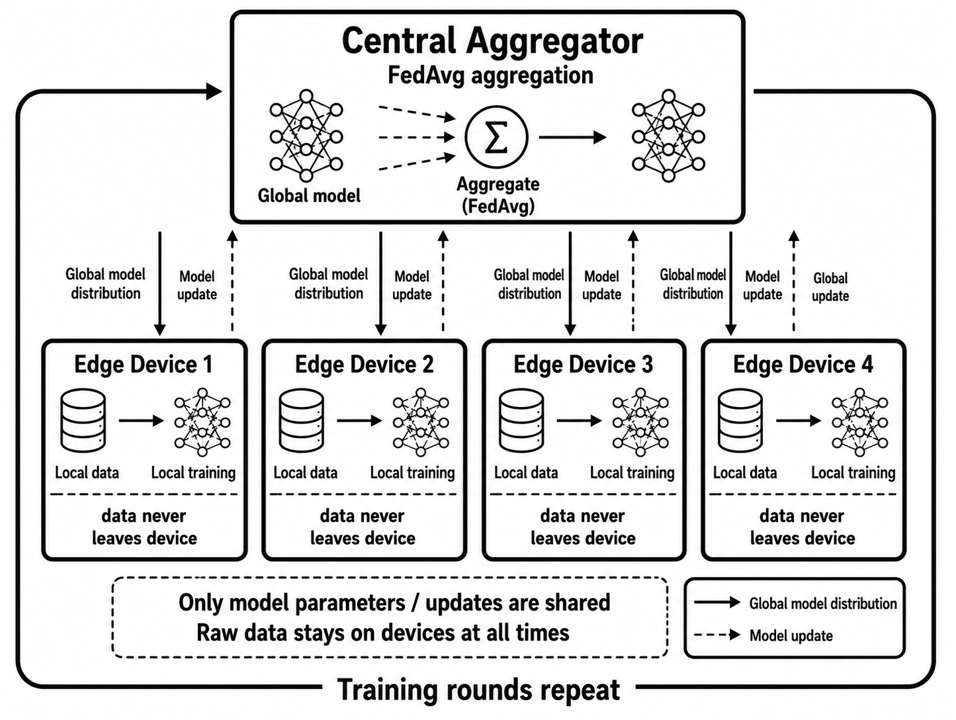
\includegraphics[width=0.95\textwidth]{figures/Picture4.png}
    \caption{Federated learning workflow. Devices train locally on data that
    never leaves the device and transmit only model updates, which the aggregator
    combines by federated averaging into an improved global model.}
    \label{fig:fl-workflow}
\end{figure}

Federated learning also aligns naturally with a tiered trust architecture. Local
model training occurs at or near the devices, while the aggregation and the
recording of accepted updates occur at a better-resourced tier, which mirrors the
separation between a fast device-facing layer and a coordinating layer developed
later in this work.

\subsection{Convolutional and Recurrent Modelling}
\label{subsec:bg-cnnlstm}
The detection engine used across the systems studied here is a hybrid network
that combines a one-dimensional convolutional stage with a recurrent stage. The
design is motivated by the structure of industrial network traffic, which is a
sequence of flow records exhibiting two kinds of pattern at once. There are
short-range, local patterns, such as burst rates, packet-size distributions, and
protocol-flag combinations, and there are longer-range temporal dependencies
arising from periodic sensing, control loops, and attack behaviour that unfolds
over time.

A one-dimensional convolutional layer is well suited to the first kind. It slides
learnable filters across the feature sequence and extracts local patterns
efficiently, producing feature maps that summarise the salient short-range
structure of the input~\cite{ige2024state, arsalan20241d}. A pooling stage then
reduces the dimensionality of these feature maps, retaining the strongest
responses while discarding fine-grained detail, which lowers computational cost
and improves robustness to small shifts in the input. The convolutional and
pooling stages together act as a feature compressor, reducing the raw input to a
compact set of representative features.
This compressed representation has, however, no explicit memory of order beyond
the span of the filters. A recurrent layer supplies that memory. A Long
Short-Term Memory network processes the sequence step by step and maintains an
internal state through gated connections that allow it to retain relevant
information across long spans while discarding the irrelevant, which lets it
model dependencies that a convolutional layer alone cannot~\cite{krichen2025long}.

Placing these stages in sequence, convolutional feature extraction and pooling
followed by recurrent temporal modelling, produces an engine that captures both
the local signatures and the temporal evolution of industrial
traffic~\cite{bamber2025hybrid}, with a final classification stage mapping the
learned representation to a probability over the traffic
classes~\cite{amadi2026lightweight, amadi2026security}. This
convolutional-recurrent pairing is the behavioural engine common to the systems
examined in the later chapters. Figure~\ref{fig:cnn-lstm} shows the arrangement
of stages, and Table~\ref{tab:cnn-lstm-stages} summarises the function of each.
\begin{figure}[htbp]
    \centering
    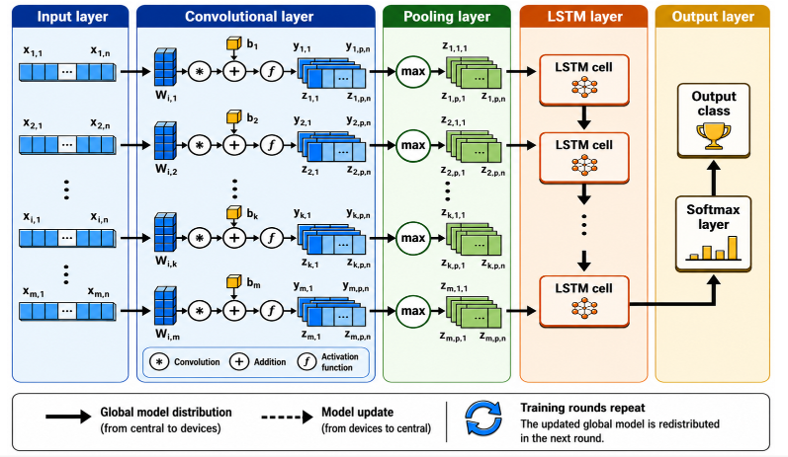
\includegraphics[width=0.89\textwidth]{figures/Picture5.png}
    \caption{Hybrid one-dimensional convolutional and recurrent detection engine.
    Convolutional and pooling layers extract and compress local features from the
    traffic sequence, the recurrent layer models temporal dependence, and a
    classification stage produces class probabilities.}
    \label{fig:cnn-lstm}
\end{figure}

\begin{table}[htbp]
\centering
\caption{Function of each stage in the hybrid convolutional-recurrent detection
engine.}
\label{tab:cnn-lstm-stages}
\small
\renewcommand{\arraystretch}{1.3}
\begin{tabular}{@{}l p{9cm}@{}}
\toprule
\textbf{Stage} & \textbf{Function} \\
\midrule
Input          & Receives the ordered sequence of network-flow features. \\
1D convolution & Extracts short-range local patterns from the feature sequence. \\
Pooling        & Reduces the dimensionality of the feature maps, retaining the strongest responses and improving robustness. \\
Recurrent (LSTM) & Models longer-range temporal dependencies across the sequence through gated memory. \\
Classification & Maps the learned representation to a probability over the traffic classes. \\
\bottomrule
\end{tabular}
\end{table}
The same architectural family appears in more than one system, instantiated on
different data. In one system it is trained on a network-intrusion benchmark and
discriminates among five traffic classes covering denial-of-service, probing,
unauthorised-access, and normal categories~\cite{amadi2026security}; in another
it is trained on a fused intrusion-detection collection and discriminates among
eight classes covering seven attack categories and one benign
class~\cite{amadi2026lightweight}. The two instances share the
convolutional-recurrent structure while differing in their datasets and their
class sets. This common lineage is noted because it recurs in the architecture
developed later.

\subsection{Trust Scoring and Revocation}
\label{subsec:bg-trust}

Detection is only useful if it drives an action. Behavioural trust management, in
which a node's trustworthiness is quantified from its observed behaviour and used
to govern its participation, is an established response to the problem of
malicious or compromised nodes in distributed and industrial
networks~\cite{ferraris2024survey}. Rather than treating security as a single
admitted-or-blocked decision made once at authentication, such schemes maintain a
continuous, evolving measure of each node's reliability and adjust it as
behaviour is observed~\cite{ullah2024deep}.

In the systems studied here, this principle is realised through a defined
sequence, illustrated in Figure~\ref{fig:trust-flow}. The behavioural engine
produces, for the device or node whose traffic was classified, a set of class
probabilities across normal and anomalous categories. These are reduced to a
single trust score in the range $[0,1]$, which is then compared against a
predefined threshold $\tau$. A device whose score satisfies $\text{score} \geq
\tau$ is treated as trustworthy and its interactions proceed; a device whose
score falls below the threshold, $\text{score} < \tau$, is flagged as anomalous.
Threshold-based conversion of a continuous anomaly signal into a discrete
security decision of this kind is a common and well-studied mechanism in network
anomaly detection~\cite{komadina2024comparing}.

A flagged device is not merely logged. It is moved through a defined lifecycle
toward isolation, in which its interactions are restricted or quarantined, and
its revocation is then recorded so that other participants no longer extend trust
to it. Anchoring trust and revocation decisions on a distributed ledger is a
recognised approach to making them tamper-evident and consistent across a
decentralised network, since no single participant can unilaterally reinstate a
revoked node~\cite{d2025blockchain}. Once the revocation is written as an
immutable ledger record, the event is propagated to the other nodes, which update
their trust state accordingly. In the present systems, this ledger-recorded and
broadcast revocation is what prevents a node excluded at one point from silently
re-entering elsewhere~\cite{amadi2026symmetric}. This coupling, from
class-probability output, to a trust score, to a threshold comparison, and then
to a ledger-recorded and propagated revocation, is the mechanism by which
learning-based detection becomes an enforceable trust decision.
Table~\ref{tab:trust-stages} summarises the role of each stage.

\begin{figure}[htbp]
    \centering
     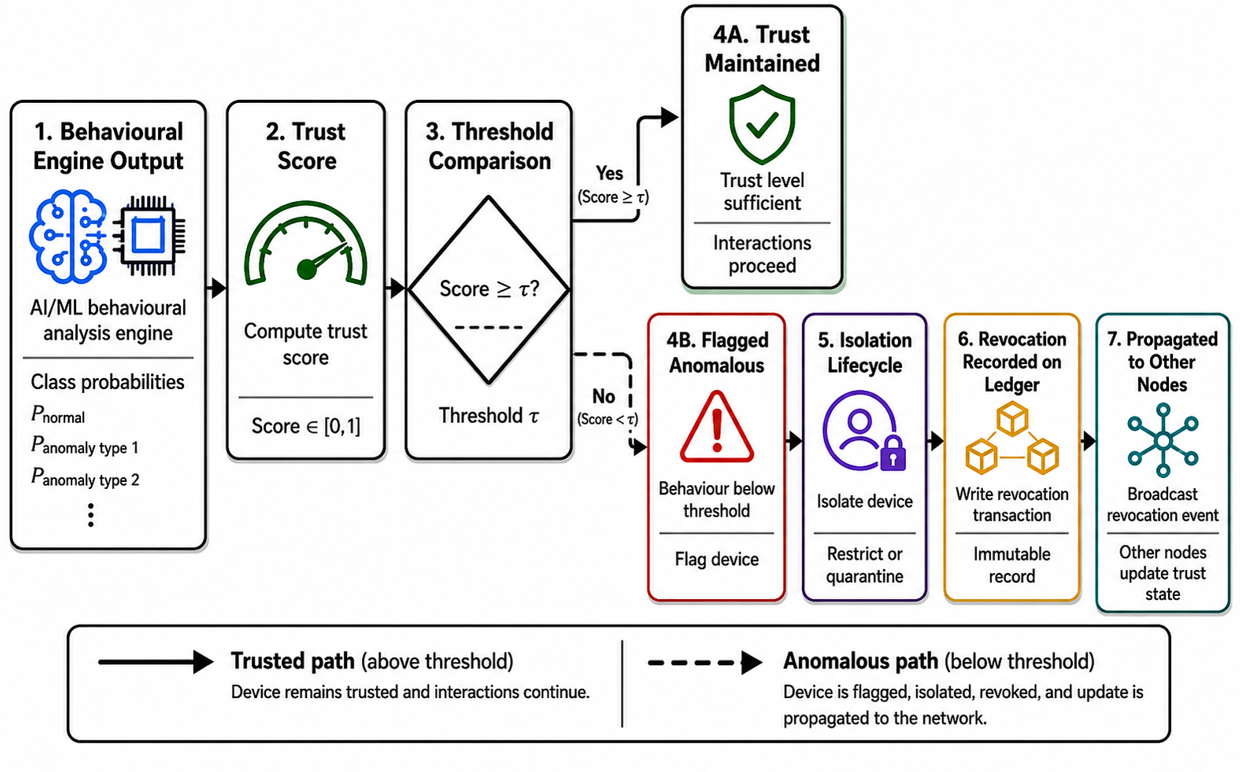
\includegraphics[width=1.05\textwidth]{figures/Picture62.PNG}
    \caption{From Detection to Enforcement: The behavioural engine's class
    probabilities yield a trust score, which is compared against the threshold $\tau$. A device with score at or above $\tau$ retains trust and its interactions proceed; a device below $\tau$ is flagged, isolated, has its revocation recorded as an immutable ledger record, and has that revocation propagated to the other nodes.}
    \label{fig:trust-flow}
\end{figure}

\begin{table}[htbp]
\centering
\caption{Stages in the trust-scoring and revocation mechanism.}
\label{tab:trust-stages}
\small
\renewcommand{\arraystretch}{1.3}
\begin{tabular}{@{}l p{8.8cm}@{}}
\toprule
\textbf{Stage} & \textbf{Function} \\
\midrule
Behavioural engine output & Produces class probabilities across normal and anomalous categories for the classified node. \\
Trust score               & Reduces the class probabilities to a single trust score in $[0,1]$. \\
Threshold comparison      & Compares the score against the threshold $\tau$ to yield a trust or anomaly verdict. \\
Trust maintained          & For a score at or above $\tau$, the device stays trusted and its interactions proceed. \\
Flagging and isolation    & For a score below $\tau$, the device is flagged anomalous and moved through an isolation lifecycle. \\
Revocation                & Writes the revocation as an immutable ledger record, making it tamper-evident. \\
Propagation               & Broadcasts the revocation so other nodes update their trust state and the device cannot re-enter elsewhere. \\
\bottomrule
\end{tabular}
\end{table}

The trust-scoring mechanism connects the learning methods of this section to the
ledger mechanisms that follow. The behavioural engine produces the evidence, the
threshold turns that evidence into a verdict, and the ledger gives the verdict
durability and reach. It is this chain, rather than any single component, that
constitutes the learning-based security foundation on which the proposed
architecture is built.




\section{AI Models and Cognitive Engines for IIoT Security}
\label{sec:ai-models}
 
From the foregoing analysis, protecting constrained, mission-critical IIoT against the threat landscape of Section~\ref{sec:bg-landscape} rests not only on the learning-based mechanisms of Section~\ref{sec:bg-learning} but on the model family that underpins them. An artificial intelligence model in this setting is a function learned from data that maps device and network observations to a security decision, and the cognitive engine is that trained model together with the calibration and scoring logic that turns its raw output into a usable, thresholded verdict. The model family is decisive, because each family carries a distinct inductive bias, data appetite, and transparency profile that fixes both what the engine can detect and how far its decision can be trusted and audited. A margin-based classifier, a convolutional feature extractor, and a graph model differ not merely in accuracy but in whether their outputs are interpretable, whether their probabilities can be calibrated, and whether their execution can be reproduced for audit. Those differences weigh most heavily under the resource and trust budget of an industrial device, where a model that cannot run within the device envelope, or whose decision cannot be reconstructed, is unsuitable however strong its benchmark accuracy.

\begin{figure}[t]
  \centering
   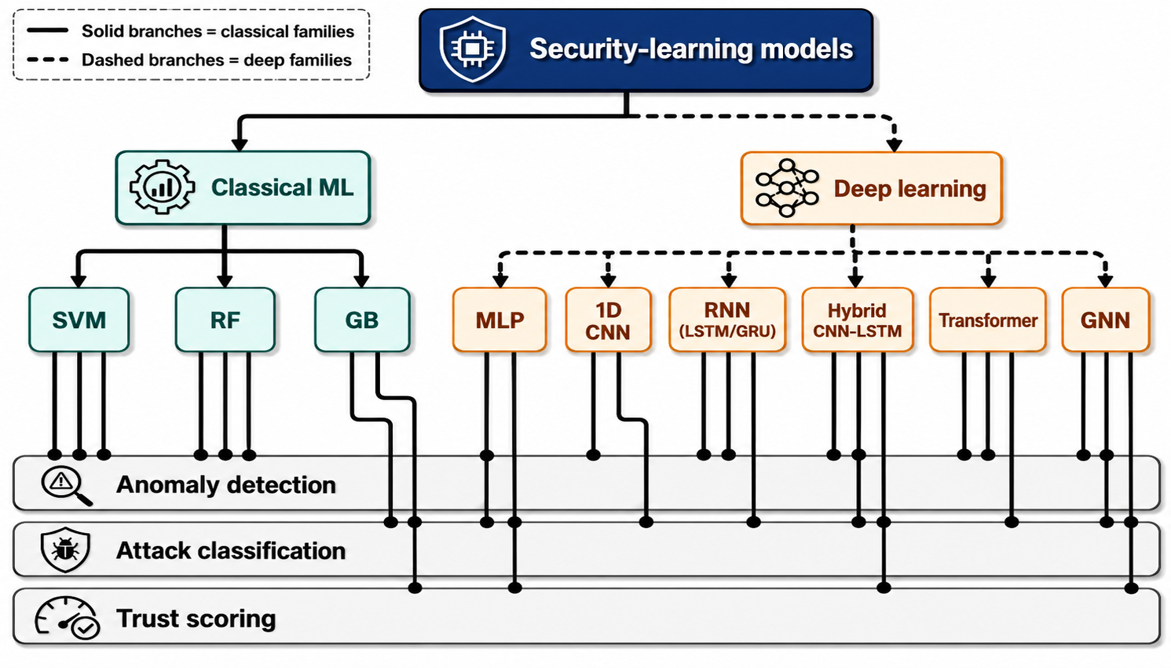
\includegraphics[width=\textwidth]{figures/Picture7.png}
  \caption{Taxonomy of AI model families for IIoT security, grouped by representational depth and mapped to the security-learning tasks each serves.}
 \label{fig:ai-taxonomy}
\end{figure}

\subsection{Model Families and the Security-Learning Tasks}
\label{subsec:model-taxonomy}
 Security learning in IIoT reduces to a small set of canonical tasks: binary anomaly detection, which separates normal from abnormal behaviour; multi-class attack classification, which assigns an observation to a specific attack category; and continuous behavioural trust scoring, which maps a device or flow to a graded reliability value. Sequential and topology-aware variants extend these tasks to telemetry that carries temporal or relational structure. Comprehensive surveys of machine-learning and deep-learning intrusion detection organise the field along these lines, cataloguing the algorithms, datasets, and attack categories that recur across deployments \cite{ali2024unveiling,kikissagbe2024machine}. A consistent finding across them is that each task admits treatment by more than one model family, so family selection is a design decision rather than a fixed consequence of the task.

\begin{table}[htbp]
  \centering
  \footnotesize
  \setlength{\tabcolsep}{4pt}
  \renewcommand{\arraystretch}{1.25}
  \caption{AI model families for IIoT security compared across the dimensions that govern trustworthy deployment. Entries are family-level properties, not measured results.}
  \label{tab:ai-family-comparison}
  \begin{tabularx}{\textwidth}{@{}
      >{\raggedright\arraybackslash}p{2.4cm}
      >{\raggedright\arraybackslash}X
      >{\raggedright\arraybackslash}X
      >{\raggedright\arraybackslash}X
      >{\raggedright\arraybackslash}X
      >{\raggedright\arraybackslash}p{1.6cm}@{}}
    \toprule
    \textbf{Model family} & \textbf{Typical role} & \textbf{Key strength} & \textbf{Key limitation} & \textbf{Transparency / trust} & \textbf{Device fit} \\
    \midrule
    Classical ML (SVM, RF, GB) & Tabular / flow anomaly and attack classification & Data-efficient; strong on engineered features; deterministic & Manual features; no native spatial or temporal modelling & High: interpretable, calibratable, reproducible & Good \\
    \addlinespace
    MLP & Nonlinear classification over features & Captures higher-order feature interactions & No structural prior; data-hungry; opaque & Low; calibratable & Moderate \\
    \addlinespace
    1D CNN & Local pattern extraction from flow or payload sequences & Parameter-efficient; translation-invariant local features & Limited long-range temporal context & Low; saliency gives partial insight & Moderate \\
    \addlinespace
    RNN / LSTM / GRU & Temporal telemetry; attack progression & Models long-range temporal dependencies & Sequential compute; hard to parallelise & Low; opaque gating & Moderate to poor \\
    \addlinespace
    Hybrid CNN-LSTM & Joint spatial-temporal behavioural detection & Combines local extraction with temporal modelling & Higher parameter and compute cost & Low; needs post-hoc XAI and calibration & Moderate \\
    \addlinespace
    Transformer / attention & Long-sequence dependency modelling & Global context; no recurrent bottleneck & Quadratic attention cost; large models & Attention gives partial insight & Poor unless offloaded \\
    \addlinespace
    GNN & Topology-aware detection (lateral movement, structure) & Encodes relational network structure & Graph construction and message-passing overhead & Low; graph explainability emerging & Poor to moderate \\
    \bottomrule
  \end{tabularx}
\end{table}

Two axes organise the family space. The first is representational depth: shallow, or classical, models operate on engineered features, whereas deep models learn representations directly from raw or lightly processed inputs. The second is the structure of the input: tabular flow statistics suit feature-based classifiers, while raw packet, byte, or event sequences reward models with spatial or temporal priors. Recent reviews of machine-learning intrusion detection for the Internet of Things adopt a comparable organisation, grouping methods by learning paradigm and by the representation each consumes \cite{manivannan2024recent}. Figure~\ref{fig:ai-taxonomy} maps the families reviewed here onto the tasks they serve, and Table~\ref{tab:ai-family-comparison} compares them across the dimensions that matter for industrial deployment.

 
The IIoT setting imposes a third axis that general machine-learning benchmarks omit: the resource and trust budget. A model that cannot execute within a Class~1 device budget, or whose outputs cannot be calibrated and audited, is unsuitable for mission-critical use, however high its benchmark accuracy. Comparative evaluations of lightweight classifiers across IoT and industrial IoT datasets show that detection quality and resource cost trade against one another, so the technique that ranks first on accuracy is rarely the one that fits the device \cite{ismail2025intrusion}, and edge-oriented designs recover deployability only through explicit optimisation such as feature reduction and model quantisation \cite{tiwari2024lightweight}. Surveys of security for resource-constrained devices treat this budget as a primary design constraint rather than a secondary concern \cite{altaibek2025survey}. This axis reweights the comparison throughout the section, favouring families whose cost and transparency remain within reach of the device rather than those that maximise raw discriminative power alone.

\subsection{Classical Machine Learning}
\label{subsec:classical-ml}
Support vector machines separate classes by the maximum-margin hyperplane in a feature space that a kernel makes implicitly nonlinear. The margin formulation performs well in high-dimensional feature spaces and captures nonlinear attack patterns through the kernel, which has made it a recurring choice for intrusion detection in the Internet of Things \cite{sama2024cutting}. Fine-tuned linear and feature-selected variants deliver accurate detection at a small model size well matched to constrained gateways \cite{azimjonov2024designing}, and hybrid rule-augmented designs extend the approach to heterogeneous IoT threat data \cite{ashraf2024hybrid}. The principal limitation is scalability: kernel training scales quadratically in the number of samples, so large corpora require dimensionality reduction or optimisation of the support-vector search to remain tractable \cite{raghunath2025pca}. Because the decision boundary depends only on a compact set of support vectors, the trained model itself remains small, which is an advantage on resource-limited hardware.
 
Tree ensembles occupy the opposite end of the classical spectrum. Random forests aggregate many decorrelated decision trees by bagging, while gradient boosting builds trees sequentially to correct the residual error of the ensemble so far. Both handle heterogeneous tabular flow features with minimal preprocessing and deliver strong performance out of the box, and lightweight tree-based detectors are for this reason widely deployed on resource-constrained IoT nodes where preprocessing and compute headroom are scarce \cite{mishra2025lirad,pandey2025lightweight}. Their split structure also yields native feature-importance measures, so an analyst can trace which features drove a decision.
 
Three properties shared across the classical family bear directly on trust. Classical models are data-efficient, deterministic under fixed seeds, and interpretable, since tree paths and linear or margin weights expose the basis of a decision \cite{abdelaziz2025enhancing}. Determinism in particular makes their outputs reproducible and therefore auditable, a property that Section~\ref{subsec:transparency-trust} develops as a trust requirement. The countervailing limitation is that classical models depend on manual feature engineering and do not natively represent the spatial or temporal structure present in raw traffic, which motivates the deep architectures reviewed next.
% ---------------------------------------------------------------------
\subsection{Deep Learning Architectures}
\label{subsec:deep-learning}
 
The multilayer perceptron is the deep baseline. Stacked nonlinear layers approximate arbitrary functions over engineered features and capture higher-order feature interactions beyond the reach of linear models, but the absence of any structural prior makes the perceptron data-hungry and its learned weights opaque \cite{cherfi2025mlp,zhao2025research}. It improves discriminative power at a direct cost in interpretability.
 
Convolutional networks introduce a spatial prior. Applied in one dimension over packet, byte, or flow sequences, convolutional filters extract local patterns through weight sharing and translation invariance, which yields parameter efficiency relative to a fully connected network of comparable capacity \cite{kumar2024deep}. The trade is a limited receptive field, so local motifs are captured well but long-range temporal context is not. Recurrent networks supply that missing temporal prior: gated variants, principally the long short-term memory and gated recurrent unit, model long-range dependencies across event sequences and so capture the progression of an attack over time, at the cost of sequential computation that resists parallelisation \cite{devendiran2024dugat}. Hybrid convolutional-recurrent models compose the two priors, placing convolutional feature extraction ahead of recurrent temporal modelling so that local structure and temporal dependency are learned jointly \cite{psychogyios2024deep}.
 
Two further families extend the design space at higher cost. Attention-based transformers replace recurrence with self-attention, modelling global dependencies across a sequence without a recurrent bottleneck and performing strongly on long inputs, but the quadratic cost of attention and the large parameter counts of these models strain constrained device budgets unless inference is offloaded \cite{ali2024empowering}. Graph neural networks encode the network as a graph of devices and flows and learn topology-aware embeddings, which suit the detection of lateral movement and structural anomalies that feature-based models miss. However, graph construction and message passing add their own overhead \cite{xu2024applying,zhong2024survey} Table~\ref{tab:task-family-fit} summarizes which families best serve each security task.
 
\begin{table}[t]
  \centering
  \caption{Security-learning tasks and the model families best suited to each.}
  \label{tab:task-family-fit}
  \renewcommand{\arraystretch}{1.3}
  \begin{tabularx}{\columnwidth}{@{}l >{\raggedright\arraybackslash}X@{}}
    \toprule
    \textbf{Security-learning task} & \textbf{Best-suited families} \\
    \midrule
    Binary anomaly detection (tabular flow)   & Classical ML; MLP \\
    Multi-class attack classification          & Tree ensembles; 1D CNN; hybrid CNN-LSTM \\
    Behavioural trust scoring (calibrated)     & Calibrated classical ML; hybrid CNN-LSTM with calibration \\
    Sequential / temporal detection            & LSTM / GRU; hybrid CNN-LSTM; transformer \\
    Topology-aware detection                   & GNN \\
    \bottomrule
  \end{tabularx}
\end{table}
 
\subsection{Transparency, Trust, and Reproducibility}
\label{subsec:transparency-trust}
Detection capability is necessary but not sufficient for trustworthy security. A recurring tension runs through the families above: representational power and transparency trade against each other, so the deep architectures that detect the subtlest attacks are also the least able to explain their alerts, while the classical models that explain themselves readily are the least expressive \cite{sharma2024explainable,mohale2025systematic}. 
Figure~\ref{fig:interpretability-tradeoff}
places the model families of this section on the interpretability capacity plane,
where the classical families occupy the high-transparency region compatible with
constrained, auditable deployment and the deep families trade that transparency for
representational power. 
Explainability methods partially close this gap for deep models. Post-hoc attribution such as feature-importance scoring and local surrogate explanation, together with attention inspection, recovers an approximate account of which inputs drove a prediction, but these explanations are estimates rather than the model's own reasoning and can be unstable across similar inputs \cite{gaspar2024explainable, wali2025explainable}. Transparency obtained this way is therefore a mitigation, not a substitute for an inherently interpretable model.

\begin{figure}[t]
  \centering
   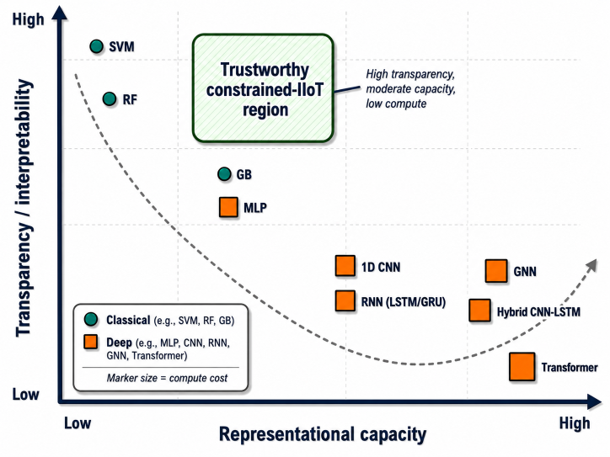
\includegraphics[width=1.05\columnwidth]{figures/Picture8.png}
 \caption{Interpretability against representational capacity for the model families of Section~\ref{sec:ai-models}. Classical families (circles) combine high transparency with moderate capacity and fall within the hatched envelope of trustworthy, auditable detection on constrained devices; deep families (squares) gain capacity at the cost of transparency and fall outside it.}
  \label{fig:interpretability-tradeoff}
\end{figure}
 
A second, distinct trust property is calibration. Behavioural trust scoring requires that a score behave as a faithful probability and not merely as a ranking, so that a fixed threshold carries a consistent meaning across devices and over time. Deep classifiers are frequently overconfident and require an explicit calibration step, such as isotonic or temperature scaling, before their outputs can support a principled threshold \cite{balanya2024adaptive, dong2025survey}. 
 
The final property is reproducibility. A security decision that cannot be reproduced cannot be independently audited, and reproducibility is far harder to guarantee for accelerated deep-learning pipelines, whose floating-point reduction orders vary across hardware, than for deterministic classical pipelines that yield bitwise-identical outputs under a fixed environment \cite{semmelrock2025reproducibility, kapoor2024reforms}. This reproducibility requirement, rather than raw accuracy alone, shapes the model choices that make verifiable IIoT security possible.
 

\section{Blockchain and Distributed Ledgers for IIoT}
\label{sec:blockchain-ledgers}
From the foregoing analysis, the behavioural trust decisions produced by the learning engines of Section~\ref{sec:ai-models} are only as dependable as the record that preserves them: a trust score, an alert, or a revocation event that can be altered after the fact cannot support accountable, auditable security in a mission-critical setting. A distributed ledger supplies that record. A blockchain is a distributed, append-only ledger in which transactions are grouped into blocks, and each block is bound to its predecessor by a cryptographic hash, so that any later modification is exposed by recomputation rather than concealed behind trust in a custodian \cite{xu2024exploring,savadatti2025survey}. The property that matters for constrained industrial deployments is not currency or decentralised finance but tamper-evident provenance: an immutable, independently checkable trail of the security-relevant events that a regulator or a partner institution must be able to reconstruct. Realising that property within a real device budget depends on three design choices, namely how the ledger is structured, who is permitted to write to it, and how distributed validators agree on its contents.


\subsection{Blocks, Hashing, and Immutability}
\label{subsec:blocks-hashing}
A block is a batch of transactions preceded by a header that records, among other fields, the cryptographic hash of the previous block. Chaining blocks by hash makes the ledger tamper-evident: altering any committed transaction changes its block hash, which invalidates the reference held by every subsequent block, so a single edit is detectable by recomputing the chain \cite{kuznetsov2024merkle}. Within a block, the transactions are summarised by a Merkle tree whose root commits to the entire set, allowing the membership of one transaction to be proven in logarithmic time without transmitting the whole block. Immutability is therefore a joint property of hash-linking and replication: the more independent validators that hold and verify the chain, the harder it becomes to rewrite history unilaterally, and the cheaper it is for any party to detect an attempt.
 
For constrained IIoT the cost of this guarantee is the binding concern. Full replication and continuous verification exceed the memory and energy budgets of low-class devices, and storing raw industrial payloads on-chain is infeasible at operational data rates. The standard resolution is to keep payloads off-chain and commit only their cryptographic digests to the ledger, so that integrity is certified without the ledger bearing the data volume \cite{eren2025security}.
 
\subsection{Permissioned and Permissionless Ledgers, and Smart Contracts}
\label{subsec:permissioned-contracts}
Ledgers differ in who may append to them. A permissionless ledger admits anonymous participants and resists censorship, but it pays for open membership with limited throughput and probabilistic finality, in which a committed block is only ever overwhelmingly, never certainly, final. A permissioned ledger restricts write access to a vetted set of validators, which yields higher throughput and deterministic finality at the cost of a narrower trust base. For constrained, mission-critical IIoT, the permissioned model is the natural fit, because an industrial consortium has identifiable members, contractual accountability, and regulatory obligations that an anonymous network cannot satisfy, and because deterministic finality aligns with the timing guarantees such systems require\cite{lahbib2024blockchain,bobde2024enhancing}.
 
Smart contracts extend a ledger from a passive record into an active policy layer. A smart contract is self-executing code stored on-chain and run identically by every validator, so its outcome is deterministic and independently verifiable rather than dependent on any single party \cite{wu2024comprehensive,wei2024survey}. This is the mechanism by which the behavioural policies such as a trust threshold, a revocation rule, or an access decision can be enforced on-chain: the same logic that scores a device can be encoded as contract logic that records, and acts on, the resulting verdict without a trusted intermediary. The contract does not improve the accuracy of the decision; it makes the decision and its consequences auditable.
 
\subsection{Consensus Families under Resource Constraints}
\label{subsec:consensus-families}
Consensus is the mechanism by which distributed validators agree on a single canonical ledger state despite faults and adversaries, and the families in use differ sharply in cost and finality. Proof-of-Work secures agreement through a computational puzzle and offers only probabilistic finality at very high energy cost. Proof-of-Stake replaces computation with economic stake, which lowers energy demand but presupposes a token economy. The Byzantine-fault-tolerant family, exemplified by Practical Byzantine Fault Tolerance, delivers deterministic finality and tolerates a bounded fraction of Byzantine validators, but its all-to-all messaging scales quadratically and so limits the practical validator-set size. Proof-of-Authority dispenses with both puzzles and stake: a small set of vetted authorities produce blocks in a fixed or rotating order, achieving deterministic finality at negligible energy cost~\cite{jain2025survey}. Table~\ref{tab:consensus-comparison} sets these families side by side on membership, finality, and fitness for a constrained industrial ledger, and shows why the choice narrows toward authority-based consensus once energy cost and deterministic finality are treated as hard requirements rather than preferences.

\begin{table}[t]
  \centering
  \footnotesize
  \setlength{\tabcolsep}{4pt}
  \renewcommand{\arraystretch}{1.25}
  \caption{Consensus families against the constraints of a permissioned industrial ledger. Entries are inherent mechanism properties, not measured results.}
  \label{tab:consensus-comparison}
  \begin{tabularx}{\columnwidth}{@{}
      >{\raggedright\arraybackslash}p{3.0cm}
      >{\raggedright\arraybackslash}p{2.1cm}
      >{\raggedright\arraybackslash}p{2.4cm}
      >{\raggedright\arraybackslash}X@{}}
    \toprule
    \textbf{Mechanism} & \textbf{Membership} & \textbf{Finality} & \textbf{Fit for constrained IIoT} \\
    \midrule
    Proof-of-Work                      & Permissionless & Probabilistic                  & Unsuitable; energy budget alone rules it out \\
    \addlinespace
    Proof-of-Stake                     & Permissionless & Near-final (variant-dependent) & Limited; presumes a token economy \\
    \addlinespace
    PBFT (BFT family)                  & Permissioned   & Deterministic                  & Small validator sets only (quadratic messaging) \\
    \addlinespace
    Proof-of-Authority                 & Permissioned   & Deterministic                  & Well suited to closed consortia \\
    \addlinespace
    Proof-of-Authority-and-Association & Permissioned   & Deterministic                  & Adds reliability-weighted, self-healing validators \\
    \bottomrule
  \end{tabularx}
\end{table}
The implications for constrained IIoT are direct. The computational puzzle of Proof-of-Work is categorically incompatible with low-class energy budgets; Proof-of-Stake assumes an economic layer that industrial consortia rarely possess; and the probabilistic finality of both conflicts with mission-critical determinism. Byzantine-fault-tolerant consensus restores determinism but bounds the validator set through its messaging cost. Proof-of-Authority therefore emerges as the practical basis for a permissioned industrial ledger, subject to one weakness that the next subsection addresses: a static authority set assumes its authorities remain both honest and available.
 
\subsection{Reliability-Aware Consensus: PoA\textsuperscript{2} and SAM+}
\label{subsec:poa2-sam}
Static Proof-of-Authority treats every authority as permanently trustworthy, so a single compromised or offline authority degrades both liveness and safety. Reliability-aware consensus removes that assumption by making authority dynamic. Proof-of-Authority-and-Association augments each validator's fixed authority with a reliability score that reflects its recent operational consistency: a block is accepted once the weighted signatures of the active validators cross an acceptance threshold, and validators are promoted from or demoted to a standby set according to a moving average of their signing history, with a gap condition between the least reliable active and the most reliable standby validator triggering replacement~\cite{kim2025proof}.
The result is a self-healing validator set that tolerates degraded authorities without surrendering the deterministic finality that constrained, mission-critical operation requires. A companion association management scheme, SAM+, maintains validator membership under changing reliability by governing how nodes join, associate, and are retired from the active set~\cite{kim2025integrating}.

These mechanisms operate over a layered permissioned ledger whose structure separates high-frequency operational commitments from the low-frequency, high-value records that must remain externally checkable. Figure~\ref{fig:purechain-layers} shows that layered organisation as a four-stage pipeline: constrained clients emit signed model-update metadata; a fast validation layer absorbs high-frequency updates with lightweight checks; the PoA\textsuperscript{2} consensus layer enforces signature, timestamp, and access-control verification to reach deterministic agreement; and an immutable anchor layer preserves only the finalised, low-frequency records that must remain externally auditable. Reading the pipeline left to right makes the division of labour explicit: frequent operations are absorbed where they are cheap, while the anchor layer is reserved for the few events whose external verifiability justifies their cost.

\begin{figure}[t]
  \centering
  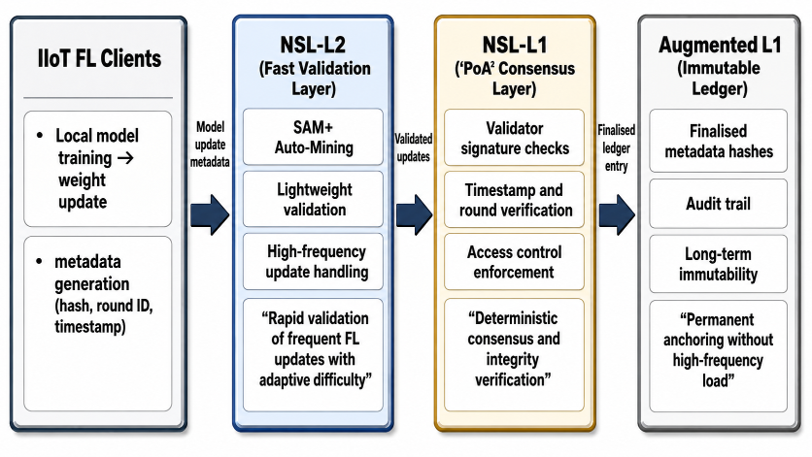
\includegraphics[width=0.95\columnwidth]{figures/Picture9.png}
  \caption{Layered structure of a permissioned industrial ledger, separating the fast layer that records high-frequency operational commitments from the layer that anchors low-frequency, high-value events for external verification.}
  \label{fig:purechain-layers}
\end{figure}

% 

\section{Hybrid Ledger Architectures and Trust Partitioning}
\label{sec:hybrid-ledgers}

From the foregoing analysis, the permissioned ledger of Section~\ref{sec:blockchain-ledgers}, secured by reliability-aware consensus, delivers the fast and deterministic finality that constrained industrial operation requires, but it confines trust to the members of the consortium: an external regulator or partner institution must ultimately take the consortium's word for the integrity of its own records. A single public ledger inverts the problem, offering verification that rests on no single institution while being unable to absorb high-frequency industrial event rates within a realistic device budget. No single ledger satisfies both the speed-and-cost constraint and the external-verifiability constraint at once. Hybrid ledger architectures resolve the tension by combining more than one ledger, and the principle that governs how work is divided between them is trust partitioning: each operation is placed on the layer whose trust model and cost profile match the operation's frequency and value.

\subsection{The Hybrid Ledger Pattern}
\label{subsec:hybrid-pattern}
The hybrid pattern pairs a fast permissioned layer with a public anchoring layer. The permissioned layer records the bulk of operational activity, while the public layer receives only periodic, compact commitments that bind the permissioned state to an externally verifiable record. The scaling literature formalises this as a Layer-1 and Layer-2 relationship, in which a Layer-2 batches many operations and commits a single proof or root to a Layer-1 chain, so that the committed state inherits Layer-1 security at a small fraction of its per-operation cost\cite{rebello2024survey}. The arrangement need not sit within one system: cross-chain and interoperability mechanisms, including relays, notary schemes, and hash-locking, move commitments between heterogeneous ledgers that were never designed to interoperate\cite{hassan2025sok}. Table~\ref{tab:ledger-types} contrasts the public, permissioned, and hybrid options on the properties that decide where an operation belongs.

Across these variants the recurring idea is separation by frequency and value: operations that occur often are kept where they are cheap, and records that must be trusted by outsiders are committed where outsiders can check them. The pattern is therefore defined less by a particular technology than by the placement decision it enforces.

\subsection{Trust Partitioning as an Architectural Principle}
\label{subsec:trust-partitioning}
Read only as a performance optimisation, the fast-plus-anchor split is a caching argument. Read as a trust argument, it is more consequential. The high-frequency behavioural operations of a constrained deployment, such as telemetry, model-update metadata, and intra-consortium validation, carry a trust requirement that the known, vetted validators of a permissioned layer already satisfy, so placing them there sacrifices nothing that an external party needs. The low-frequency, high-value events, such as audit roots, revocation records, and cross-institution commitments, carry a trust requirement that the consortium cannot satisfy on its own account, and only a genuinely public anchor makes them checkable by a party outside the consortium \cite{wang2024public}. Trust partitioning is the discipline of routing each class of event to the layer that can actually vouch for it.

This layered organisation is not merely convenient; layered and tiered blockchain designs have been analysed as a structural response to the resource and trust asymmetries of industrial deployments~\cite{li2025blockchain,song2024novel}, and the structural necessity of such a reference architecture is argued in the systematic review that scaffolds this work (Chapter~\ref{ch:review}). What the principle does not by itself settle is whether a single partitioning rule can hold across different ledger substrates; that question is taken up in Section~\ref{subsec:hybrid-instances}.

\subsection{Instances Across Ledger Substrates}
\label{subsec:hybrid-instances}
The same partitioning principle admits realisations that differ in substrate. Within a single hybrid ledger, a permissioned network-service layering can absorb high-frequency validation while a public augmented Layer-1 preserves the anchored record, so the split is internal to one design. Across two distinct ledgers, a permissioned Hyperledger Fabric network can carry operational transactions while a public Ethereum network holds the anchoring commitments, so the split is a boundary between technologies. Across compute tiers, a federated edge-and-cloud arrangement can partition work by where it is produced and where it must be preserved.

Presented here only as building blocks, these realisations establish three facts: that the pattern exists, that it is a partitioning of trust rather than merely of load, and that more than one substrate can carry it. Whether they express a single, substrate-independent trust-partitioning principle is a question this section deliberately leaves open. Figure~\ref{fig:hybrid-pattern} shows the pattern in its generic form, with a fast permissioned layer feeding periodic commitments to a public anchor.

\begin{table}[t]
  \centering
  \footnotesize
  \setlength{\tabcolsep}{4pt}
  \renewcommand{\arraystretch}{1.25}
  \caption{Public, permissioned, and hybrid ledgers compared on the properties that decide where an operation belongs, after~\cite{al2024shbf}. Entries are inherent properties, not measured results.}
  \label{tab:ledger-types}
  \begin{tabularx}{\columnwidth}{@{}
      >{\raggedright\arraybackslash}p{2.3cm}
      >{\raggedright\arraybackslash}p{2.3cm}
      >{\raggedright\arraybackslash}X
      >{\raggedright\arraybackslash}X@{}}
    \toprule
    \textbf{Ledger type} & \textbf{Write access} & \textbf{Prospects} & \textbf{Limitations} \\
    \midrule
    Public (permissionless) & Open, anonymous & Externally verifiable without a trusted operator; censorship-resistant & Low throughput; probabilistic finality; high cost and energy \\
    \addlinespace
    Permissioned (private / consortium) & Restricted to vetted validators & High throughput; deterministic finality; accountable membership & Trust confined to the operator or consortium; not externally verifiable on its own \\
    \addlinespace
    Hybrid (tiered) & Layered: permissioned plus public & Combines fast permissioned operation with public verifiability; partitions work by frequency and value & Added integration and cross-layer coordination complexity \\
    \bottomrule
  \end{tabularx}
\end{table}



\begin{figure}[t]
  \centering
  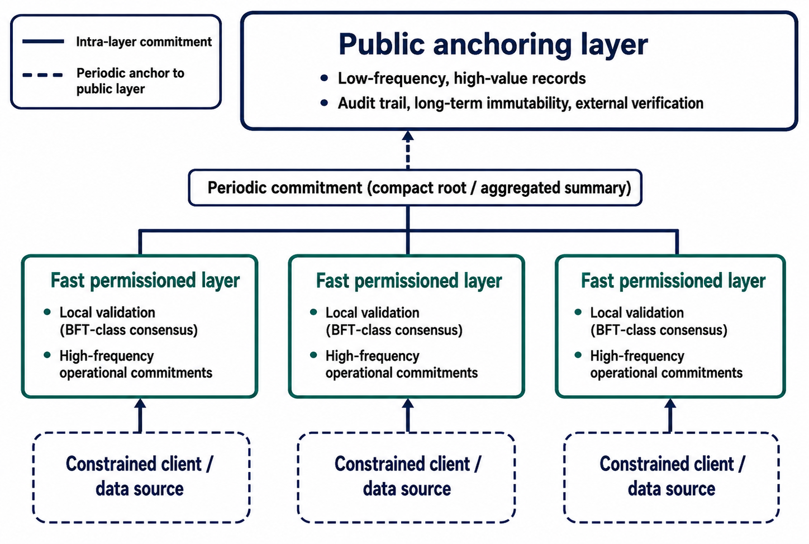
\includegraphics[width=0.99\columnwidth]{figures/Picture10.png}
  \caption{Generic hybrid ledger pattern. Fast permissioned layers absorb high-frequency operational activity and periodically commit a compact root to a public anchoring layer, which preserves low-frequency, high-value records for verification by parties outside the consortium.}
  \label{fig:hybrid-pattern}
\end{figure}



\section{The Case for Trust-Partitioned Security}
\label{sec:case}
Generally, the security of a constrained industrial deployment cannot be delegated to any single mechanism. Section~\ref{sec:bg-landscape} showed that the threat surface is broad and its consequences physical rather than merely informational. Sections~\ref{sec:bg-learning} and~\ref{sec:ai-models} showed that behavioural detection can be made accurate, calibrated, and auditable, but only within a model whose cost and transparency fit the device that must run it. Section~\ref{sec:blockchain-ledgers} showed that a permissioned ledger under reliability-aware consensus can render those decisions tamper-evident at a deterministic and affordable cost. Section~\ref{sec:hybrid-ledgers} showed that a hybrid ledger, governed by trust partitioning, can reconcile the speed a device can afford with the external verifiability a regulator or partner institution demands. Each of these is necessary; none is sufficient on its own.

Read together, they converge on a single requirement: security for constrained, mission-critical IIoT must be at once behavioural, verifiable, and affordable. Behavioural, because static signatures cannot anticipate the attacks that now matter. Verifiable, because a decision that cannot be independently reconstructed cannot be trusted by the parties who bear its consequences. Affordable, because a mechanism that exceeds the device budget is never deployed, whatever its merits on paper. Trust partitioning is the principle that holds these three in tension without sacrificing any of them, by routing each operation to the layer that can both bear its cost and vouch for its trust, so that speed is not bought at the price of verifiability nor verifiability at the price of feasibility.

A fourth requirement is temporal, and it is easily overlooked. The identities and commitments that anchor an industrial system are long-lived: equipment fielded today may still be in service, and still trusted, a decade from now. An adversary therefore need not break current cryptography today, but can record protected traffic now and decrypt it once a cryptographically relevant quantum computer exists, so the effective migration deadline is set by the lifetime of the data rather than by the arrival of the machine \cite{singh2024managing}. The standardisation of post-quantum key encapsulation and signatures, noted in Section~\ref{sec:bg-landscape}, makes migration possible; what makes it hard is that lattice-based schemes carry larger keys and ciphertexts than the elliptic-curve schemes they replace, pressing on exactly the memory and transmission budgets that already constrain these devices \cite{castiglione2024integrating}. Post-quantum resistance is thus not a separate concern bolted onto the architecture but another face of the same affordability problem: the cryptographic anchor of trust must be quantum-resistant and compact at once.

Beneath all four requirements runs the resource budget, which is less a requirement than a filter applied to every other choice. It is the budget that rules out proof-of-work, that forbids unbounded validator sets, that penalises opaque high-capacity models, and that turns post-quantum migration from a configuration change into a design problem. A proposal that sets the budget aside is not conservative but inapplicable, and much of the apparent disagreement across the mechanisms surveyed here dissolves once the budget is treated as binding rather than negotiable.

Taken together, these requirements describe a target that none of the mechanisms in isolation reaches: a security architecture that is behavioural in its detection, tamper-evident in its record, trust-partitioned in its structure, post-quantum in its cryptographic anchor, and viable within a real device budget throughout. The case for trust-partitioned security is the case that these properties are jointly necessary and jointly attainable, rather than a menu from which one selects. Whether existing practice already offers such an architecture, and if it does not, precisely where and why it falls short, cannot be settled from the selective reading of a background chapter. It calls for the systematic, reproducible review undertaken in Chapter~\ref{ch:review}, where the distance between these requirements and what current approaches deliver is measured and the resulting gap made precise.

\chapter{Review of Related Works}
\label{Chapter_3}
\section{Methodology for Review of Literature}
\label{sec:review-method}
A defensible account of where existing security architectures fall short of the requirements set out in Section~\ref{sec:case} cannot rest on a selective reading of convenient sources. It requires a search that is reproducible, criteria that are stated in advance, and a corpus assembled without the bias that undermines a narrative survey. The review reported in this chapter therefore adopts the Preferred Reporting Items for Systematic Reviews and Meta-Analyses (PRISMA) framework~\cite{prisma}, which prescribes a transparent, stage-by-stage procedure for identifying, screening, and selecting studies and for reporting the exclusions made at each stage. The phenomenon of interest is the intersection at which the thesis is positioned: learning-driven detection, blockchain-anchored provenance, and post-quantum protection, examined under the resource constraints of industrial deployment rather than in the abstract.

The search was conducted across five databases, namely IEEE Xplore, Scopus, Web of Science, the ACM Digital Library, and SpringerLink, between 1 March and 5 April 2025, targeting publications from 2020 to 2025. Restricting the corpus to this window is deliberate rather than incidental: the convergence of hybrid ledgers, learning-based security, and post-quantum standardisation that the thesis addresses emerged substantially within this period, so an earlier window would dilute relevance rather than improve coverage. Six core terms structured the query, namely ``hybrid blockchain'', ``digital twin'', ``data-sharing security'', ``cross-chain'', ``privacy-preserving blockchain'', and ``energy-efficient consensus'', each adapted to the query syntax of the individual databases. Table~\ref{tab:search-strings} records the exact string issued to each database, so that the search can be reproduced rather than merely described.

\subsection{Inclusion and Exclusion Criteria}
\label{subsec:review-criteria}

Eligibility was decided against criteria fixed before screening began, so that inclusion reflected the protocol rather than the reviewer's expectation. A study was included if it satisfied all of the following:
\begin{itemize}
  \item published in a peer-reviewed journal or conference proceedings;
  \item published within the 2020 to 2025 window;
  \item directly concerned with hybrid blockchain technology in the context of secure, resource-aware data sharing;
  \item written in English.
\end{itemize}
A study was excluded if it lacked conceptual depth, reported neither empirical nor analytical validation, or addressed blockchain applications outside the defined scope. Non-original items such as editorials and letters were removed without further assessment.

\subsection{Article Selection Results}
\label{subsec:review-results}

The search returned 512 records. Automated and manual deduplication reduced these to 412 unique records. Screening of titles and abstracts removed 162 irrelevant publications, leaving 250 for full-text assessment, of which 134 were excluded for insufficient conceptual depth, absence of validation, or scope mismatch. The final corpus comprised 116 studies, 99 of them quantitative and 17 qualitative. Figure~\ref{fig:prisma-flow} presents the complete PRISMA selection flow, with the count retained and the reasons for exclusion recorded at each stage.

The composition of the retained corpus locates the field in time and domain. Studies published in 2023 and 2024 account for 62 of the 116 works, a little over half, which confirms the rapid growth of the area; 2021 and 2022 contribute 29 works, and 2020 together with 2025 the remaining 25. Peer-reviewed journal articles dominate the corpus, with conference proceedings and book chapters forming a smaller share, indicating a research area maturing toward archival publication. By application domain, healthcare and the Internet of Medical Things, industrial and cyber-physical systems, transport and the Internet of Vehicles, and energy systems are the most frequently addressed, with construction, supply chain, and civic systems adding further diversity and the remainder spanning multi-domain or general settings. Figure~\ref{fig:review-stats} summarises this distribution.

\subsection{Quality Assessment and Bias Evaluation}
\label{subsec:review-quality}

Each retained study was assessed against five quality criteria: clarity of research objectives; reproducibility of the proposed method or system design; traceability of results, meaning whether performance claims such as throughput, latency, or energy efficiency were supported by experimental data or formal analysis; relevance to hybrid blockchain and resource-aware data sharing; and acknowledgement of study-level limitations. Failure on objectives, reproducibility, or relevance was grounds for exclusion at full-text review.

Five sources of bias were addressed directly rather than left implicit. Publication bias was mitigated by spanning five databases across multiple publishers and venues. Language bias is acknowledged, since the English-only restriction may omit relevant non-English work, although English dominates peer-reviewed research in this area over the target period. Selection bias was controlled by applying the inclusion and exclusion criteria consistently across both screening phases, with ambiguous cases resolved by re-evaluation. Recency bias is inherent to the 2020 to 2025 scope but deliberate, given that the field emerged largely within it. Aggregation bias, arising from heterogeneous performance metrics across studies, is acknowledged as a residual limitation: every quantitative figure carried into this review is attributed to its primary source and is not treated as a cross-study validated or normalised estimate.

% ---------------------------------------------------------------------
% TABLE 3.x — search strings per database (reproduce from the DT paper's Table 3)
% ---------------------------------------------------------------------
\begin{table}[t]
  \centering
  \footnotesize
  \setlength{\tabcolsep}{4pt}
  \renewcommand{\arraystretch}{1.3}
  \caption{Search string issued to each database, adapted to the query syntax of the source.}
  \label{tab:search-strings}
  \begin{tabularx}{\columnwidth}{@{}
      >{\raggedright\arraybackslash}p{2.4cm}
      >{\raggedright\arraybackslash}X@{}}
    \toprule
    \textbf{Database} & \textbf{Search string} \\
    \midrule
    IEEE Xplore   & (``digital twin'' OR ``DT'') AND (``hybrid blockchain'' OR ``public private blockchain'') AND (security OR privacy OR interoperability) \\
    \addlinespace
    Scopus        & TITLE-ABS-KEY(``digital twin'' AND ``hybrid blockchain'') AND (privacy OR security OR consensus) \\
    \addlinespace
    Web of Science & TS=(``digital twin'' AND ``hybrid blockchain'') AND TS=(security OR privacy) \\
    \addlinespace
    ACM DL        & [[Abstract: ``digital twin''] AND [``hybrid blockchain'']] AND [keywords: security OR consensus] \\
    \addlinespace
    SpringerLink  & (``digital twin'' + ``hybrid blockchain'' + security OR privacy) in Title or Abstract \\
    \bottomrule
  \end{tabularx}
\end{table}

\begin{figure}[t]
  \centering
  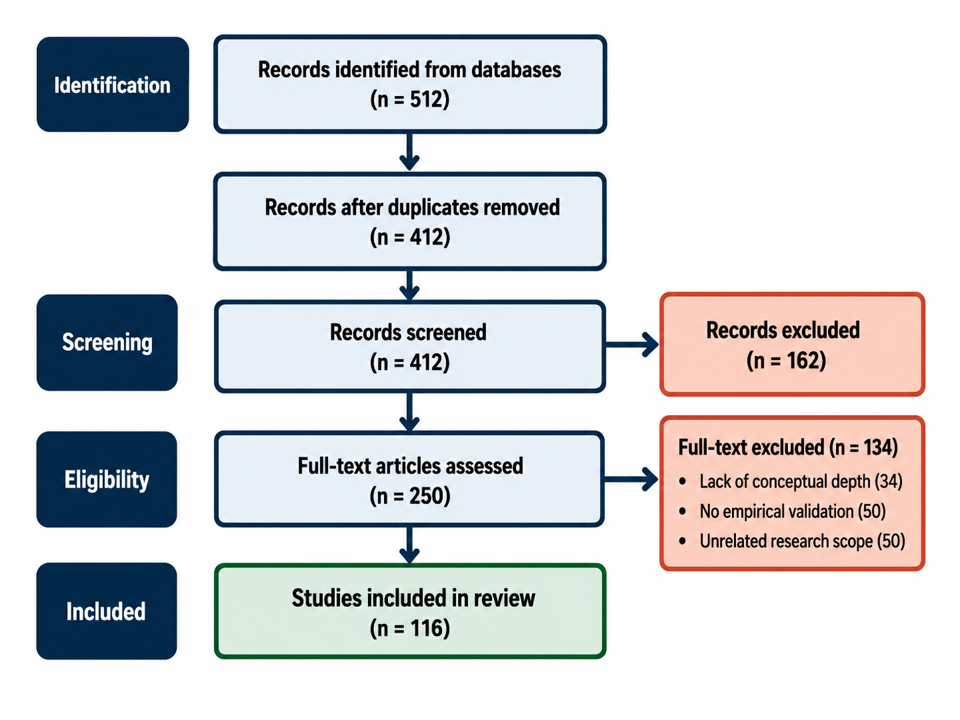
\includegraphics[width=0.9\columnwidth]{figures/Picture11.png}
  \caption{PRISMA 2020 flow diagram showing record identification, screening, eligibility assessment, and inclusion, with the count retained and the reason for exclusion recorded at each stage: 512 records identified, 412 after deduplication, 250 after title and abstract screening, and 116 retained after full-text assessment.}
  \label{fig:prisma-flow}
\end{figure}


\begin{figure}[t]
  \centering
  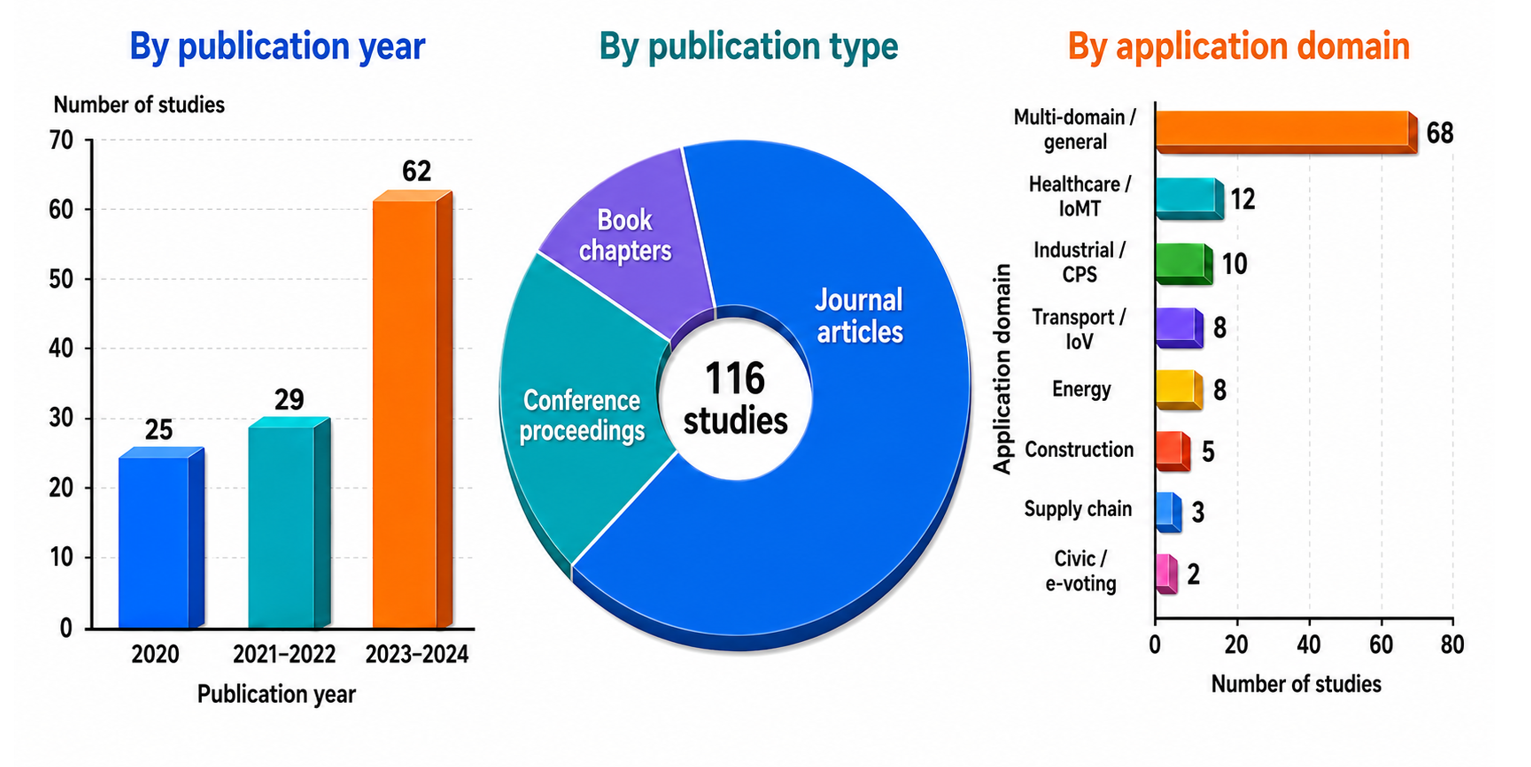
\includegraphics[width=0.97\columnwidth]{figures/Picture122.png}
   \caption{Distribution of the 116 retained studies. Left: by publication year, with more than half of the corpus published in 2023 and 2024. Right: by application domain, with the seven most frequently addressed specific domains shown and the remaining studies grouped as multi-domain or general contexts. By publication type, peer-reviewed journal articles dominate the corpus, with conference proceedings and book chapters forming a smaller share.}
    \label{fig:review-stats}
\end{figure}


 
\section{Review of Recent Works}
\label{sec:recent-works}
 
Substantial effort has been directed at securing blockchain-enabled and digital-twin systems, and a first orientation is best obtained not from individual proposals but from the reviews that have already synthesised them. Table~\ref{tab:review-comparison} compares the most relevant prior review and survey works along the dimensions that decide whether a review speaks to the problem addressed here: whether it treats the digital-twin ecosystem (DTE) as its object, whether it engages conventional blockchain technology (CBT) or the hybrid model (HBT), whether it organises its findings through a three-dimensional lifecycle-layer-security taxonomy, whether it performs a comparative defence-gap analysis, and whether it traces each open issue to a research direction. The final three columns tell the decisive story at a glance: across every prior review, the taxonomy, defence-gap, and issue-to-direction columns are uniformly absent, and only the present review supplies all three.
 
The prior reviews fall into three groups, each capable within its remit and each limited in the same structural way. The first group treats blockchain as a broad enabler of digital twins without isolating the hybrid model as a necessary architectural response. Surveys of blockchain for digital twins~\cite{yaqoob}, of blockchain-based digital-twin trends~\cite{sabah}, of digital-twin and blockchain integration~\cite{hemdan}, and the more recent multi-domain accounts~\cite{dwivedi,Nexus} cover the pairing of the two technologies capably, but treat the choice between public, private, and hybrid ledgers as a design detail rather than as the structural pivot on which digital-twin security turns. The second group narrows to the hybrid model but not to the digital-twin setting: the one prior systematic review of hybrid blockchain platforms~\cite{alkhateeb} addresses general Internet-of-Things systems and does not engage the lifecycle-specific trade-offs that arise under real-time, high-frequency workloads. The third group reviews digital-twin architecture and enabling technologies thoroughly, in accounts of digital-twin technology and networking~\cite{maggie}, of enabling technologies and prospects~\cite{Mihai}, and of Internet-of-Digital-Twins architecture~\cite{wangbest}, but offers no security-focused synthesis, no defence-gap analysis, and no structured mapping from open issue to future direction.
 
A closer reading within these groups reinforces the point. The domain-specific reviews demonstrate real depth in their settings, of digital twins in remanufacturing supply chains~\cite{chen}, of blockchain for secure health data sharing~\cite{peng,upadrista}, of building-lifecycle management~\cite{adu}, of security in Industry~4.0 digital twins~\cite{elhajj}, and of data fusion in the energy sector~\cite{jiang}, yet their security treatment stays bound to the application rather than abstracted into a reusable architectural principle. The recent multi-domain reviews extend coverage and currency, and one adds case-study evidence alongside its systematic method~\cite{christos,Nexus}, but none introduces the three analytical dimensions on which a trust-partitioned architecture must be assessed. Several of these works are systematic in method~\cite{chen,alkhateeb,upadrista,adu,christos,Nexus,elhajj,jiang}, which confirms that methodological rigour is not what the field lacks; what it lacks is a security-focused synthesis organised around the hybrid, trust-partitioned model.
 
Read together, these reviews establish that the field has matured and that the pairing of blockchain with digital-twin and industrial systems is now well surveyed. What none provides, as the three rightmost columns of Table~\ref{tableX} make explicit, is a security-focused synthesis that isolates the hybrid, trust-partitioned model as a structural response, measures the defence coverage it achieves, and traces the residual gaps to the directions that would close them. That absence defines the contribution of the review reported here. The substantive state of the art on which it draws is examined next in Section~\ref{sec:soa}, before the resulting gaps are consolidated in Section~\ref{sec:review-gap}.

\begin{table*}[!htbp]
\centering
\setlength{\arrayrulewidth}{0.8mm}
\caption{Comparison of Selected Related Works}
\resizebox{\textwidth}{!}{%
\begin{tabular}{llllccccccccc}
\hline
\textbf{Ref} & \textbf{Year} & \textbf{Review Target Area} & \textbf{Review Remarks} & \textbf{Systematic Review} & \textbf{Case Studies} & \textbf{DTE} & \textbf{CBT} & \textbf{HBT} & \textcolor{black}{\textbf{3D Tax.}} & \textcolor{black}{\textbf{Defense Gap}} & \textcolor{black}{\textbf{Issue--Dir. Trace.}} \\
\hline
\cite{yaqoob} & 2020 & Non-specific & Secure manufacturing & \ding{55} & \checkmark & \checkmark & \checkmark & \ding{55} & \ding{55} & \ding{55} & \ding{55} \\
\midrule
\cite{maggie} & 2021 & Non-specific & Technology of DT & \ding{55} & \ding{55} & \checkmark & \ding{55} & \ding{55} & \ding{55} & \ding{55} & \ding{55} \\
\midrule
\cite{chen} & 2021 & Supply chains & DT in remanufacturing & \checkmark & \ding{55} & \checkmark & \ding{55} & \ding{55} & \ding{55} & \ding{55} & \ding{55} \\
\midrule
\cite{peng} & 2022 & Health & BT secure data sharing & \ding{55} & \ding{55} & \ding{55} & \checkmark & \ding{55} & \ding{55} & \ding{55} & \ding{55} \\
\midrule
\cite{alkhateeb} & 2022 & IoT & Adoption of HBT & \checkmark & \ding{55} & \ding{55} & \ding{55} & \checkmark & \ding{55} & \ding{55} & \ding{55} \\
\midrule
\cite{Mihai} & 2022 & Non-specific & Realization of DT & \ding{55} & \checkmark & \checkmark & \ding{55} & \ding{55} & \ding{55} & \ding{55} & \ding{55} \\
\midrule
\cite{sabah} & 2022 & Non-specific & Blockchain-based DT & \ding{55} & \ding{55} & \checkmark & \checkmark & \ding{55} & \ding{55} & \ding{55} & \ding{55} \\
\midrule
\cite{RUI} & 2023 & Non-specific & BT-based data sharing & \ding{55} & \ding{55} & \ding{55} & \checkmark & \ding{55} & \ding{55} & \ding{55} & \ding{55} \\
\midrule
\cite{hemdan} & 2023 & IoT Systems & DT and BT integration & \ding{55} & \ding{55} & \checkmark & \checkmark & \ding{55} & \ding{55} & \ding{55} & \ding{55} \\
\midrule
\cite{upadrista} & 2023 & Health & BT for data sharing & \checkmark & \ding{55} & \ding{55} & \checkmark & \ding{55} & \ding{55} & \ding{55} & \ding{55} \\
\midrule
\cite{wangbest} & 2023 & Non-specific & IoDT architecture & \ding{55} & \ding{55} & \checkmark & \ding{55} & \ding{55} & \ding{55} & \ding{55} & \ding{55} \\
\midrule
\cite{adu} & 2023 & Post-construction & Building management & \checkmark & \ding{55} & \checkmark & \checkmark & \ding{55} & \ding{55} & \ding{55} & \ding{55} \\
\midrule
\cite{dwivedi} & 2024 & Multi-domain & BT enabled DT & \ding{55} & \ding{55} & \checkmark & \checkmark & \ding{55} & \ding{55} & \ding{55} & \ding{55} \\
\midrule
\cite{christos} & 2024 & Smart Industry & BT and DT integration & \checkmark & \checkmark & \checkmark & \checkmark & \ding{55} & \ding{55} & \ding{55} & \ding{55} \\
\midrule
\cite{Nexus} & 2024 & Multi-domain & Effects of BT on DT & \checkmark & \ding{55} & \checkmark & \checkmark & \ding{55} & \ding{55} & \ding{55} & \ding{55} \\
\midrule
\cite{elhajj} & 2024 & Industry 4.0 & Security in DT & \checkmark & \ding{55} & \checkmark & \ding{55} & \ding{55} & \ding{55} & \ding{55} & \ding{55} \\
\midrule
\cite{jiang} & 2024 & Energy sector & Data fusion with DT & \checkmark & \ding{55} & \checkmark & \ding{55} & \ding{55} & \ding{55} & \ding{55} & \ding{55} \\
\midrule
\textbf{Ours} & \textbf{2026} & \textbf{Multi-domain} & \textbf{HBT secure data sharing} & \checkmark & \checkmark & \checkmark & \checkmark & \checkmark & \checkmark & \checkmark & \checkmark \\
\hline
\end{tabular}}
\label{tableX}
\scriptsize
\checkmark~Considered; $\times$~Not considered; \textcolor{black}{DTE: Digital Twin Ecosystem; CBT: Conventional Blockchain Technology; BT: Blockchain Technology; HBT: Hybrid Blockchain Technology.} \textcolor{black}{3D Tax.: Three-dimensional lifecycle-layer-security taxonomy; Defense Gap: Comparative defense coverage and residual gap analysis; Issue--Dir.~Trace.: Explicit open-issue to future research direction traceability.}
\end{table*}



\begin{sidewaystable}
\centering
\caption{Comparison of selected prior review works.}
\label{tab:review-comparison}
\renewcommand{\arraystretch}{1.25}
\setlength{\tabcolsep}{6pt}
\begin{tabular}{@{}l l l l cccccccc@{}}
\toprule
\textbf{Ref} & \textbf{Year} & \textbf{Target Area} & \textbf{Review Remarks}
 & \rotatebox{90}{\textbf{Systematic review}}
 & \rotatebox{90}{\textbf{Case study}}
 & \rotatebox{90}{\textbf{DTE}}
 & \rotatebox{90}{\textbf{CBT}}
 & \rotatebox{90}{\textbf{HBT}}
 & \rotatebox{90}{\textbf{3D Tax.}}
 & \rotatebox{90}{\textbf{Defence gap}}
 & \rotatebox{90}{\textbf{Issue--Dir.}} \\
\midrule
\cite{yaqoob}    & 2020 & Non-specific      & Secure manufacturing   & \ding{55} & \checkmark & \checkmark & \checkmark & \ding{55} & \ding{55} & \ding{55} & \ding{55} \\
\cite{maggie}    & 2021 & Non-specific      & Technology of DT       & \ding{55} & \ding{55} & \checkmark & \ding{55} & \ding{55} & \ding{55} & \ding{55} & \ding{55} \\
\cite{chen}      & 2021 & Supply chains     & DT in remanufacturing  & \checkmark & \ding{55} & \checkmark & \ding{55} & \ding{55} & \ding{55} & \ding{55} & \ding{55} \\
\cite{peng}      & 2022 & Health            & BT secure data sharing & \ding{55} & \ding{55} & \ding{55} & \checkmark & \ding{55} & \ding{55} & \ding{55} & \ding{55} \\
\cite{alkhateeb} & 2022 & IoT               & Adoption of HBT        & \checkmark & \ding{55} & \ding{55} & \ding{55} & \checkmark & \ding{55} & \ding{55} & \ding{55} \\
\cite{Mihai}     & 2022 & Non-specific      & Realization of DT      & \ding{55} & \checkmark & \checkmark & \ding{55} & \ding{55} & \ding{55} & \ding{55} & \ding{55} \\
\cite{sabah}     & 2022 & Non-specific      & Blockchain-based DT    & \ding{55} & \ding{55} & \checkmark & \checkmark & \ding{55} & \ding{55} & \ding{55} & \ding{55} \\
\cite{RUI}       & 2023 & Non-specific      & BT-based data sharing  & \ding{55} & \ding{55} & \ding{55} & \checkmark & \ding{55} & \ding{55} & \ding{55} & \ding{55} \\
\cite{hemdan}    & 2023 & IoT Systems       & DT and BT integration  & \ding{55} & \ding{55} & \checkmark & \checkmark & \ding{55} & \ding{55} & \ding{55} & \ding{55} \\
\cite{upadrista} & 2023 & Health            & BT for data sharing    & \checkmark & \ding{55} & \ding{55} & \checkmark & \ding{55} & \ding{55} & \ding{55} & \ding{55} \\
\cite{wangbest}  & 2023 & Non-specific      & IoDT architecture      & \ding{55} & \ding{55} & \checkmark & \ding{55} & \ding{55} & \ding{55} & \ding{55} & \ding{55} \\
\cite{adu}       & 2023 & Post-construction & Building management     & \checkmark & \ding{55} & \checkmark & \checkmark & \ding{55} & \ding{55} & \ding{55} & \ding{55} \\
\cite{dwivedi}   & 2024 & Multi-domain      & BT enabled DT          & \ding{55} & \ding{55} & \checkmark & \checkmark & \ding{55} & \ding{55} & \ding{55} & \ding{55} \\
\cite{christos}  & 2024 & Smart Industry    & BT and DT integration  & \checkmark & \checkmark & \checkmark & \checkmark & \ding{55} & \ding{55} & \ding{55} & \ding{55} \\
\cite{Nexus}     & 2024 & Multi-domain      & Effects of BT on DT    & \checkmark & \ding{55} & \checkmark & \checkmark & \ding{55} & \ding{55} & \ding{55} & \ding{55} \\
\cite{elhajj}    & 2024 & Industry 4.0      & Security in DT         & \checkmark & \ding{55} & \checkmark & \ding{55} & \ding{55} & \ding{55} & \ding{55} & \ding{55} \\
\cite{jiang}     & 2024 & Energy sector     & Data fusion with DT    & \checkmark & \ding{55} & \checkmark & \ding{55} & \ding{55} & \ding{55} & \ding{55} & \ding{55} \\
\midrule
\textbf{This review} & \textbf{2026} & \textbf{Multi-domain} & \textbf{Trust-partitioned security} & \checkmark & \checkmark & \checkmark & \checkmark & \checkmark & \checkmark & \checkmark & \checkmark \\
\bottomrule
\end{tabular}

\vspace{4pt}
{\footnotesize \checkmark~considered; $\times$~not considered.
DTE: digital-twin ecosystem; CBT: conventional blockchain technology; BT: blockchain technology; HBT: hybrid blockchain technology; 3D Tax.: three-dimensional lifecycle-layer-security taxonomy; Defence gap: comparative defence coverage and residual-gap analysis; Issue--Dir.: open-issue to future-direction traceability.}
\end{sidewaystable}



\section{State-of-the-Art Approaches}
\label{sec:soa}

Three technical capabilities carry the weight of the reviewed corpus: detecting compromise as it occurs, recording that detection in a form that cannot later be altered, and protecting the record against an adversary whose capabilities grow over time. The approaches that address each are surveyed in turn, with attention to what they achieve and to the limitation that each leaves for the next to resolve.

\subsection{Learning-Based Detection and Trust Scoring}
\label{subsec:soa-learning}

Learning-based detection has displaced signature matching as the dominant approach to industrial intrusion detection, because the attacks that matter in operational technology rarely match a known signature and often manifest only as a drift in behaviour. The reviewed corpus divides along the representational depth of the model, and the division carries the familiar trade-off between interpretability and capacity into concrete system designs.

Classical machine-learning detectors remain widely deployed for industrial traffic, where tree ensembles and margin-based classifiers operating on engineered flow features deliver strong accuracy at a computational cost that constrained gateways can absorb, and with decision logic an operator can inspect\cite{majidian2024optimizing}. Their weakness is equally documented: performance depends on the quality of hand-engineered features, degrades under the distribution drift that characterises evolving industrial networks, and falls away on temporally extended or previously unseen attack patterns that the feature set was not designed to capture \cite{agate2024driftaware,ennaji2025adversarial}.

Deep detectors raise the achievable ceiling by learning representations directly from traffic. Convolutional detectors extract spatial structure from packet and flow encodings \cite{alshehri2024selfattention, hassini2024endtoend}; recurrent detectors built on long short-term memory and gated recurrent units model the temporal dependence of an attack that unfolds across a session\cite{chen2024xgboostlstm, raeiszadeh2024realtime}; and hybrid convolutional-recurrent detectors combine the two to capture spatiotemporal behaviour that neither recovers alone\cite{chen2025cnnlstm,anwer2025federated}. More expressive still, graph-based detectors exploit the topology of an industrial network to localise compromise \cite{villegas2025dynamic, deng2025edgefeatured}, and attention-based models extend the temporal reach of detection across longer horizons\cite{akuthota2025transformer,ishtiaq2025cstafnet}. The recurring limitation across this family is not accuracy but cost and accountability: higher-capacity models demand memory, energy, and labelled data that constrained deployments cannot always supply, and their decisions resist the explanation and the bitwise reproducibility that an audited setting requires.

A parallel strand addresses the distribution of training itself. Federated detectors keep raw industrial data on the premises that generate it, exchanging only model updates, which answers the confidentiality and data-sovereignty constraints of multi-site industrial operation\cite{lee2025lightweight, mao2025fedinnid}. The approach introduces its own exposure, since the update channel invites model-poisoning and the heterogeneity of industrial data across sites degrades convergence\cite{quyen2025fedkd, sun2025personalized}. A further strand recognises that a detection verdict is only actionable if its confidence is trustworthy, and applies calibration and explanation so that a reported probability reflects an observed rate and a flagged event can be justified\cite{shoukat2025trustids, pal2025calibrated}; yet such work rarely extends to making the calibrated verdict independently reproducible or externally checkable.

These strands converge on behavioural trust scoring, the thread most relevant to the architecture developed later. Rather than emitting a one-shot alert, trust-scoring approaches maintain a continuous, decaying estimate of a device's or a peer's reliability, updated from observed behaviour and used to gate access or trigger revocation\cite{anwer2025tead, awan2025stacktrust}. Reputation and trust-management schemes formalise how such scores accrue, decay, and drive revocation across a network of interacting nodes\cite{bampatsikos2025trustscore, wang2025continuous}. The limitation that unites the entire section is now visible: learning-based detection can be made accurate, temporally aware, privacy-preserving, and even calibrated, but the trust verdict it produces is computed and stored wherever the model runs, so it remains exactly as mutable as its host. A verdict that can be altered after the fact cannot anchor an accountable security decision, which is the requirement that ledger-based provenance, examined in Section~\ref{subsec:soa-ledger}, exists to meet.





\subsection{Blockchain and Consensus for IIoT Provenance}
\label{subsec:soa-ledger}

The limitation that closed the previous subsection, a trust verdict as mutable as the host that computes it, is precisely what distributed-ledger provenance exists to remove. The reviewed corpus applies blockchain to industrial systems less as a currency than as an integrity layer, committing security-relevant events to a record that no single participant can silently revise. The concrete systems divide by the trust model of the ledger they build on and by the consensus that keeps that ledger consistent.

Permissioned ledgers dominate the industrial setting, because a vetted consortium supplies the accountable membership and the throughput that anonymous public chains cannot. Systems in this class anchor device identities, access decisions, and audit records on a consortium chain, giving an external party a tamper-evident trail to reconstruct \cite{samriya2025workload,salam2026secure}, and several couple the ledger directly to intrusion detection so that a flagged event is committed rather than merely logged \cite{song2025hybrid,peng2025bctdics}. Their recurring cost is throughput and storage: committing at industrial event rates strains both the consensus path and the on-chain footprint, so raw telemetry cannot be placed on the ledger without exhausting the very budgets that constrain the devices \cite{xiong2025sharding,ding2025dcstorage}.

Consensus is where the resource tension concentrates. The energy and latency of proof-of-work rule it out for constrained operation, which has driven industrial designs toward Byzantine-fault-tolerant and authority-based protocols that reach deterministic finality at a fraction of the cost \cite{zheng2025trbft,wu2025dbpbft}. Reputation-aware and reliability-weighted consensus variants extend this by adjusting a validator's influence according to its observed behaviour, so that a degraded or compromised authority loses weight without halting the network \cite{zeng2025ibft, xiong2025reputation}. Even these, however, assume a validator set small enough to coordinate, which bounds the scale at which a single permissioned ledger can operate and leaves open how high-frequency operation and externally verifiable finality are to be reconciled at once.

A further body of work turns the ledger from a passive record into an active control point through smart contracts, encoding access policy, revocation, and audit logic that executes identically across validators \cite{li2025hyperiiot,dildar2025endtoend}. This is the mechanism by which a trust decision from the detection layer can be made not only recorded but enforced, and by which revocation can be triggered without a trusted intermediary \cite{he2026bfldias,xia2026ecroa}. The limitation that unites the section is one of placement rather than capability: a single ledger that is fast enough for operational commitment is rarely public enough for external verification, and one that is public enough for verification is rarely fast enough for operational commitment. Resolving that tension is the concern of the hybrid and tiered designs examined in Section~\ref{subsec:soa-hybrid}.


\subsection{Hybrid Ledgers and Post-Quantum Protection}
\label{subsec:soa-hybrid}

The placement tension that closed the previous subsection, that a ledger fast enough for operational commitment is rarely public enough for external verification, is the problem hybrid and tiered ledger designs set out to dissolve rather than merely trade away. The reviewed corpus resolves it not by choosing between the two ledger types but by composing them, assigning high-frequency operation to a fast permissioned layer and externally checkable finality to a slower public anchor, with a defined path between the two.

Tiered and layered architectures place a permissioned ledger close to the devices, where consensus is cheap and finality is quick, and periodically commit a compact digest of that ledger's state to a second, more widely trusted chain \cite{ullah2025mbid,banitalebi2025edblsd}. The mechanism that joins the layers is cross-chain anchoring: a hash or Merkle root computed on the fast layer is written to the anchor chain, so that a compact commitment on the public ledger stands in for the full history held below, and any later dispute can be settled against it without replaying the whole record \cite{oleszkiewicz2026cross, correa2026decoupling}. This composition is what allows a single system to satisfy operational speed and external verifiability at once, and it is the structural pattern on which a trust-partitioned architecture depends. Its cost is added coordination and the security of the bridge itself, since a compromised or poorly designed cross-chain link becomes the weakest point of the combined system \cite{zhou2025bridgeguard, mukherjee2025double}.

A verifiability that is sound today is not thereby sound for the lifetime of an industrial deployment, and this is where the second concern of the subsection enters. The cryptographic signatures and hashes that make a ledger tamper-evident rest on assumptions that a cryptographically relevant quantum computer would overturn, and the harvest-now-decrypt-later posture means that records anchored today can be targeted once such capability exists\cite{reddy2025quantum, revathi2025enhancing}. Work in this area migrates ledger signatures and identity credentials to lattice-based and other quantum-resistant primitives, and reports the throughput and footprint consequences of doing so on the ledger path\cite{hussain2025quantum,hao2025efficient}. The unresolved difficulty is that quantum-resistant primitives carry larger keys and signatures than the schemes they replace, which collides directly with the memory and energy budgets of the constrained devices that the fast layer is meant to serve\cite{hanna2025comprehensive,cruz2025measuring}.

Across the three subsections, a consistent shape emerges. Learning-based detection supplies an accurate but mutable trust verdict; ledger provenance makes that verdict immutable but forces a choice between speed and public verifiability; hybrid and tiered ledgers dissolve that choice but inherit a bridge to secure and a quantum horizon to survive. No single reviewed system carries all three concerns at once under the resource budget of constrained industrial operation. Section~\ref{sec:review-gap} consolidates the specific gaps this leaves and states the questions the remainder of the work addresses.



\section{Summary of Review and Research Gaps}
\label{sec:review-gap}
The review assembled in this chapter set out to locate, against a reproducible corpus rather than a convenient selection, where existing security architectures fall short of a clear requirement: that trustworthy security for constrained industrial operation must be at once behavioural, verifiable, and affordable, and must remain so against an adversary whose cryptographic reach grows with time. The state of the art advances each of these properties in isolation and, read across its three strands, exposes a coherent set of gaps that no reviewed system closes together.
The first gap concerns the mutability of the trust verdict. Learning-based detection has become accurate, temporally aware, privacy-preserving through federation, and in the best work calibrated and explainable. Yet the verdict it produces is computed and stored wherever the model runs, and is therefore alterable by whoever controls that host. Accuracy without immutability cannot underwrite an accountable security decision, and the reviewed detectors do not, on their own, make their output tamper-evident.

The second gap concerns placement. Ledger provenance supplies the immutability that detection lacks, but the reviewed systems force a choice between two incompatible virtues. A permissioned ledger fast enough for high-frequency behavioural commitment is not public enough to be externally verifiable, while a public ledger open enough for external verification is not fast enough for operational commitment. No single-ledger design surveyed reconciles operational speed with independent verifiability within a constrained budget.
The third gap concerns durability and its cost. Hybrid and tiered ledgers dissolve the placement dilemma by composing a fast permissioned layer with a public anchor joined through cross-chain anchoring, and this is the structural pattern on which a partitioned architecture depends. The composition, however, inherits two unresolved liabilities: the cross-chain link becomes the weakest point of the combined system, and the tamper-evidence of the anchored record rests on cryptography that a quantum adversary would defeat, so that post-quantum migration becomes mandatory yet collides with the memory and energy budgets of the very devices the fast layer serves.

A fourth gap cuts across the other three. The reviewed corpus contains detectors, ledgers, and hybrid designs, but no single system carries behavioural detection, immutable and externally verifiable provenance, and quantum-resilient protection at once under the resource envelope of constrained industrial hardware. Where composed systems do appear, the organising principle behind them is demonstrated on a single implementation, leaving open whether trust-partitioning is a substrate-independent principle or an artefact of one design. The evaluations that would settle this, spanning detection performance, resource overhead, blockchain-side cost, and quantum resilience together, are largely absent.

These gaps motivate the five research questions that organise the remainder of the work. The first follows from the second and third gaps taken together: can trust be partitioned across a hybrid ledger, so that high-frequency behavioural validation is handled on a fast permissioned layer while low-frequency, high-value events such as identity anchoring, audit, and revocation are committed to a separate anchoring layer, and does this partitioning deliver trustworthy security within real device resource budgets? The second follows from the first gap and the affordability requirement: can lightweight artificial-intelligence behavioural trust scoring operate inside the compute, memory, and energy budgets of real constrained IIoT devices without sacrificing detection performance? The third follows from the durability half of the third gap: can post-quantum-resilient identity and credential delivery be achieved on such hardware without prohibitive latency or bandwidth cost? The fourth follows from the fourth gap: does the trust-partitioning principle hold across distinct ledger substrates, rather than being an artefact of a single implementation? The fifth follows from the accountability thread that runs through all four gaps: under adversarial conditions, can behavioural trust scoring with decay-based revocation reliably isolate a misbehaving node while the hybrid-ledger architecture sustains dependable detection performance?
Answering these questions requires an architecture that reconciles scalability, speed, and security while carrying out validation and anchoring within the resource limits of industrial edge hardware. The design of that architecture, and the trust-partitioning principle that organises it, is the subject of the next chapter.

\chapter{Proposed STRATA Architecture}
%Research Direction and System  Methodology
% \pagenumbering{arabic}

\Large
\label{Chapter_4}

The STRATA framework secures resource-constrained industrial devices by partitioning trust across tiered layers, so that speed, verifiability, and cost are each served where they are cheapest to obtain rather than traded against one another on a single ledger. Its construction proceeds through four elements: (a) a behavioural trust-scoring stratum that scores device conduct in real time on a fast permissioned layer, (b) a consensus and coordination stratum that finalises validated behaviour under permissioned consensus, (c) a public anchoring stratum that commits compact proofs to an open layer for external audit, and (d) two cross-cutting planes that carry quantum-resilient identity, revocation, and post-quantum protection across all three strata. This chapter details the design and operational logic of each element, the resource-aware placement principle that binds them, and the two ledger substrates on which the framework is realised. Figure~\ref{fig:strata-arch} presents the overall architecture, with the three strata separated by the trust-partition boundary and the two planes spanning them.


\begin{figure}[t]
  \centering
  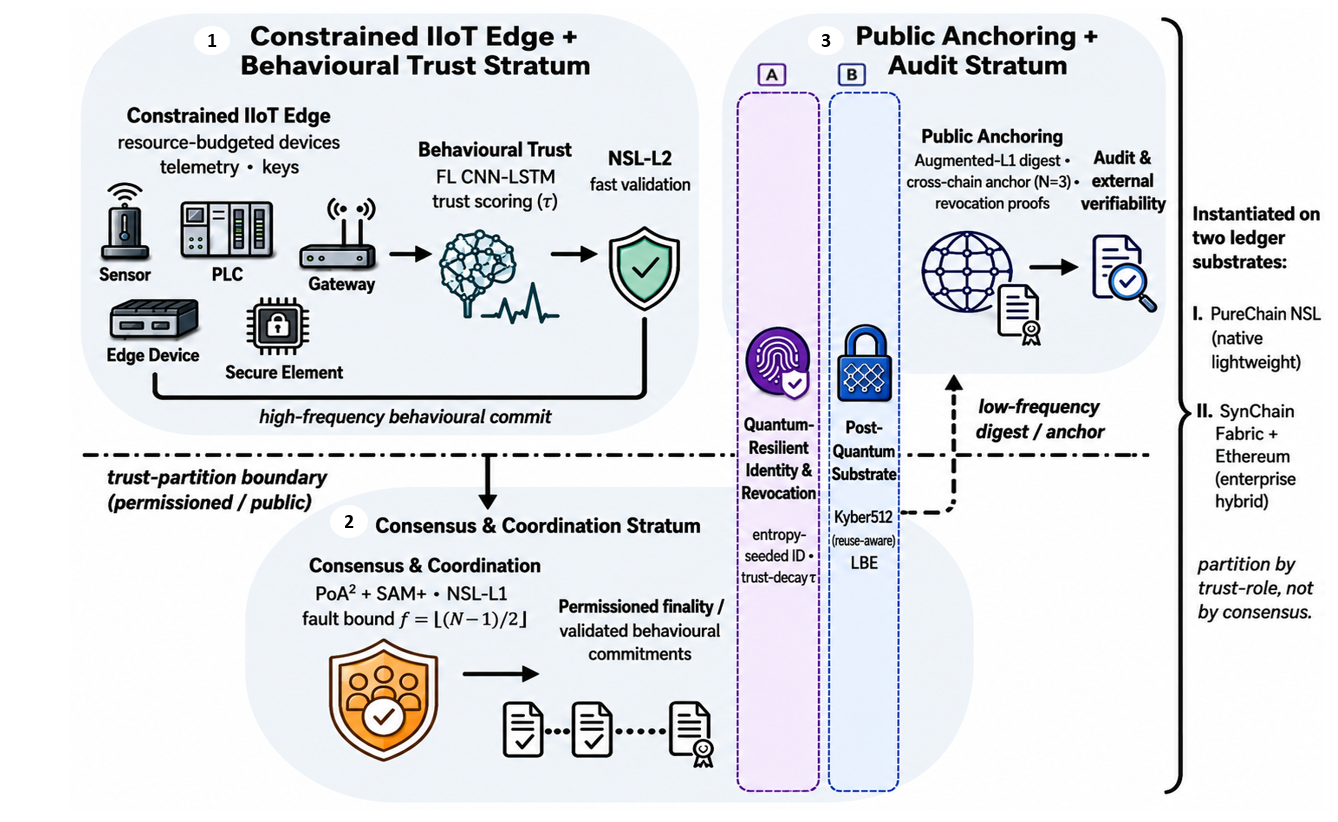
\includegraphics[width=\textwidth]{figures/Picture133.PNG}
 \caption[STRATA framework architecture]{Architecture of the proposed STRATA
framework. The solid arrow marks the high-frequency behavioural commitment
retained inside the permissioned domain, and the dashed arrow the
low-frequency digest that crosses the trust-partition boundary to the public
anchor. Planes~A and~B span all three strata, and the tiered core is realised
on two ledger substrates, PureChain NSL and SynChain Fabric+Ethereum,
partitioning by trust-role rather than by consensus mechanism.}
  \label{fig:strata-arch}
\end{figure}

The objective of STRATA is the greatest attainable trustworthy security that a constrained deployment can sustain, obtained by assigning each security operation to the stratum whose trust characteristics match it. Let $\sigma$ denote such an assignment of operations to strata, $\mathcal{T}(\sigma)$ the trustworthiness it delivers, and $\mathcal{R}(\sigma)$ its resource footprint. The design solves

\begin{equation}
\label{eq:strata-objective}
\sigma^{\star} \;=\; \arg\max_{\sigma}\; \mathcal{T}(\sigma)
\quad \text{subject to} \quad
\mathcal{R}_{\text{edge}}(\sigma) \le \mathcal{B}_{\text{edge}},
\;\;
\mathcal{R}_{\text{chain}}(\sigma) \le \mathcal{B}_{\text{chain}},
\end{equation}

where $\mathcal{B}_{\text{edge}}$ is the compute, memory, and energy budget of the constrained edge and $\mathcal{B}_{\text{chain}}$ the throughput and storage budget of the ledger. Trustworthiness combines behavioural detection fidelity with anchored verifiability,

\begin{equation}
\label{eq:strata-trust}
\mathcal{T}(\sigma) \;=\; \sum_{i=1}^{n} \big[\, w_{s}\, s_i \;+\; w_{\upsilon}\, \upsilon_i(\sigma) \,\big],
\end{equation}

in which $s_i \in [0,1]$ is the accumulated behavioural trust score of device $d_i$ (Section~\ref{sec:plane-a}), $\upsilon_i(\sigma)\in\{0,1\}$ indicates whether that device's security-relevant events are anchored and hence externally verifiable, and $w_{s}, w_{\upsilon}$ weight detection against verifiability. Equation~\eqref{eq:strata-objective} states the problem the strata jointly solve: the permissioned strata raise $s_i$ within the edge budget while the anchoring stratum raises $\upsilon_i$ within the ledger budget, so that neither term improves by exhausting the resources of the other. A centralised or single-ledger arrangement, by contrast, must satisfy both budgets on one layer and therefore cannot maximise either without violating the constraint that constrained hardware imposes.



\section{The Trust-Partitioning Principle and System Model}
\label{sec:strata-principle}

Security, speed, and scalability compete on any ledger placed on constrained industrial hardware, and no single-ledger design reconciles all three within a real device budget. STRATA resolves the tension by reassignment rather than compromise: each security responsibility is placed on the layer whose trust characteristics match it, so operations demanding speed run where consensus is cheap and operations demanding public accountability run where verification is open. This converts the trilemma from a balance to be struck into a placement to be solved, and it is the principle from which the rest of the framework follows.

The placement rests on a single observation. Security-relevant operations differ not only in what they protect but in the trust profile they require. A behavioural trust update issued many times per second needs deterministic, low-cost validation and tolerates a closed validator set. An identity revocation or an audit commitment occurs rarely, carries high value, and must be verifiable by parties outside the operating consortium. Treating both alike forces one ledger to be fast and public at once, which constrained budgets do not permit. Partitioning treats them differently by design.

\begin{definition}[Trust-partitioning]
\label{def:trust-partition}
A security architecture is trust-partitioned if every security-relevant operation $e$ is assigned to exactly one stratum according to its trust-role $\kappa(e)=(\phi_e,\nu_e,\xi_e)$, where $\phi_e$ is the operation's frequency, $\nu_e$ its value, and $\xi_e$ its required verifiability scope, such that high-frequency, low-value operations with consortium-internal verifiability are confined to a fast permissioned stratum, low-frequency, high-value operations with external verifiability are committed to a public anchoring stratum, and a single well-defined interface transfers state between the two.
\end{definition}

The partition is drawn by trust-role, not by consensus mechanism. This distinction carries the framework's generality: the same assignment of operations to strata can be realised on substrates whose consensus protocols differ entirely, a property developed in Section~\ref{sec:strata-substrates}.

\subsection{System Model}
\label{subsec:strata-sysmodel}

The framework serves a set $\mathcal{D}=\{d_1,\dots,d_n\}$ of resource-constrained industrial devices, each generating telemetry and holding key material at the constrained edge. Above this base, security responsibility divides across three strata and two cross-cutting planes.

The behavioural trust stratum scores device conduct in real time. A lightweight federated CNN--LSTM intrusion-detection engine evaluates network and metadata behaviour and emits a per-window trust score $q_i \in [0,1]$, committed at device rate on the fast permissioned layer (NSL-L2) so that the verdict is recorded rather than left on the host that computed it. The full detection design is given in Section~\ref{sec:strata-trust}.

The consensus and coordination stratum finalises those commitments. Permissioned finalisation uses the Proof-of-Authority-and-Association protocol with the Smart Auto-Mining Plus mechanism on the coordination layer (NSL-L1), tolerating up to $f=\lfloor (N-1)/2 \rfloor$ faulty or unavailable validators for $N$ authorities. Deterministic finality bounds the latency of a behavioural decision without exposing it publicly.

The public anchoring stratum carries only what external accountability requires. Compact digests of finalised state and revocation proofs cross the trust-partition boundary and are committed to an open layer (Augmented-L1), cross-chain-anchored to a public chain where interoperability demands it. Payloads never cross; only proofs do, which preserves confidentiality while enabling open verification. The anchoring design appears in Section~\ref{sec:strata-anchor}.

Two planes span the strata rather than residing in any one. The identity and revocation plane, detailed in Section~\ref{sec:strata-identity}, binds each device to an entropy-seeded identity and governs revocation by a trust-decay law, so a verdict raised in the trust stratum propagates to a revocation proof anchored in the public stratum. The post-quantum plane protects credentials and anchored records with lattice-based primitives against both classical and quantum adversaries. Figure~\ref{fig:strata-arch} places both planes as vertical elements to indicate this span.

\subsection{Verifiability Under Partitioning}
\label{subsec:strata-theorem}

A partition is sound only if confining an operation to the permissioned side preserves its public verifiability. The following establishes that partitioning meets this condition.

\begin{theorem}[Verifiability preservation]
\label{thm:verifiability}
Let a security-relevant event $e$ be finalised within the permissioned strata, and let its digest $H(e)$ be anchored on the public stratum under an immutable ledger, where $H$ is collision-resistant. Then any party with access to the public stratum alone can verify the integrity of $e$, and the partition introduces no loss of verifiability relative to committing $e$ in full on the public stratum.
\end{theorem}

\begin{proof}[Proof sketch]
Verifying $e$ means confirming that the copy presented to a verifier is the one finalised. A verifier recomputes $H(e')$ from a presented $e'$ and compares it to the anchored $H(e)$; equality holds if and only if $e'=e$, except with negligible probability under collision resistance. Immutability of the public stratum guarantees the anchored value cannot be altered after commitment, so the reference is trustworthy. Integrity of $e$ is therefore verifiable from the public stratum without access to the permissioned strata. Committing $e$ publicly in full would expose the same guarantee through $e$ itself; the partition transfers only the proof $H(e)$ to the public stratum and confines the payload, so no verifiability is lost.
\end{proof}

Theorem~\ref{thm:verifiability} is the formal counterpart of the placement argument. Because the proof of integrity, not the payload, is what public accountability requires, the high-value proof is anchored publicly while the high-frequency payload stays permissioned, which is the separation Definition~\ref{def:trust-partition} prescribes. Table~\ref{tab:strata-map} sets each element of the framework against the review gap it closes and the research question it answers, so the architecture reads as a principled response to the gaps established earlier rather than a set of untested mechanisms.


\begin{table}[t]
  \centering
  \footnotesize
  \setlength{\tabcolsep}{5pt}
  \renewcommand{\arraystretch}{1.3}
  \caption{Mapping of each STRATA stratum and plane to its function, the review gap it closes, and the research question it addresses.}
  \label{tab:strata-map}
  \begin{tabularx}{\textwidth}{@{}
      >{\raggedright\arraybackslash}p{3.0cm}
      >{\raggedright\arraybackslash}X
      >{\raggedright\arraybackslash}p{2.4cm}
      >{\raggedright\arraybackslash}p{0.9cm}@{}}
    \toprule
    \textbf{Element} & \textbf{Function} & \textbf{Gap closed} & \textbf{RQ} \\
    \midrule
    Stratum~1 \newline Behavioural Trust
      & Federated CNN--LSTM behavioural trust scoring on the fast permissioned layer
      & Mutable verdict & RQ2 \\
    Stratum~2 \newline Consensus \& Coordination
      & Permissioned finalisation via PoA$^2$ and SAM+; fault bound $f=\lfloor(N{-}1)/2\rfloor$
      & Placement (speed) & RQ1 \\
    Stratum~3 \newline Public Anchoring
      & Digest anchoring and cross-chain commitment of proofs
      & Placement (public) & RQ1 \\
    Plane~A \newline Identity \& Revocation
      & Entropy-seeded identity and trust-decay revocation across strata
      & Accountability & RQ5 \\
    Plane~B \newline Post-Quantum Substrate
      & Compressed Kyber512 and lattice-based encryption for credentials and anchors
      & Quantum durability & RQ3 \\
    \addlinespace
    Dual-substrate realisation
      & Same partition on PureChain NSL and on SynChain Fabric+Ethereum
      & Substrate dependence & RQ4 \\
    \bottomrule
  \end{tabularx}
\end{table}

The strata and planes are specified individually in the sections that follow, beginning with the behavioural trust-scoring stratum. Table~\ref{tab:notation} collects the principal notation used throughout the chapter.

\begin{table}[htbp]
  \centering
  \footnotesize
  \setlength{\tabcolsep}{5pt}
  \renewcommand{\arraystretch}{1.25}
  \caption{Principal notation used in the specification of STRATA.}
  \label{tab:notation}
  \begin{tabularx}{\textwidth}{@{}
      >{\raggedright\arraybackslash}p{2.2cm}
      >{\raggedright\arraybackslash}X
      >{\raggedright\arraybackslash}p{2.6cm}@{}}
    \toprule
    \textbf{Symbol} & \textbf{Meaning} & \textbf{Introduced in} \\
    \midrule
    $\mathcal{D}$, $d_i$ & Set of constrained devices; device $i$ & Section~\ref{subsec:strata-sysmodel} \\
    $\sigma$ & Assignment of security operations to strata & Eq.~\eqref{eq:strata-objective} \\
    $\kappa(e)$ & Trust-role of operation $e$: frequency, value, verifiability scope & Definition~\ref{def:trust-partition} \\
    $q_i$ & Per-window behavioural trust score produced by Stratum~1 & Eq.~\eqref{eq:strata-flag} \\
    $\delta$ & Flag threshold applied to $q_i$ & Eq.~\eqref{eq:strata-flag} \\
    $s_i(t)$ & Accumulated device trust score maintained by Plane~A & Eq.~\eqref{eq:trust-decay} \\
    $\beta$ & Retention factor of the trust-decay law & Eq.~\eqref{eq:trust-decay} \\
    $\tau$ & Revocation threshold applied to $s_i(t)$ & Section~\ref{sec:plane-a} \\
    $S_i(t)$, $\mu_S$ & Anomaly streak counter; streak limit & Eq.~\eqref{eq:revoke-condition} \\
    $\omega_i$, $\theta$ & Validator authority weight; weighted acceptance threshold & Eq.~\eqref{eq:poa2-accept} \\
    $\rho_i(t)$, $\gamma$ & Validator reliability; reliability decay factor & Eq.~\eqref{eq:poa2-reliability} \\
    $N$, $f$ & Active validator count; tolerated faulty validators & Eq.~\eqref{eq:poa2-fault} \\
    $E$, $\lambda$ & Epoch span; verdict arrival rate & Definition~\ref{def:epoch} \\
    $R_k$, $\mathcal{C}_k$ & Epoch root; public commitment for epoch $k$ & Eqs.~\eqref{eq:merkle-root}, \eqref{eq:anchor-tuple} \\
    $\pi$ & Evidence bundle supporting a revocation & Eq.~\eqref{eq:revoke} \\
    $H(\cdot)$ & Collision-resistant hash function & Theorem~\ref{thm:verifiability} \\
    $c_{\mathrm{tx}}$, $\lambda_r$ & Fee per public commitment; revocation rate & Eq.~\eqref{eq:anchor-cost} \\
    \bottomrule
  \end{tabularx}
\end{table}

\section{The Behavioural Trust-Scoring Stratum}
\label{sec:strata-trust}
The behavioural trust-scoring stratum is where compromise is detected and turned into a committed verdict. Industrial attacks rarely match a fixed signature and usually surface only as a drift in how a device communicates, so detection here is learned from behaviour rather than matched against rules. The stratum runs a lightweight federated intrusion-detection engine at the constrained edge, scores each device's conduct as a continuous value, and writes that score to the fast permissioned layer, so the trust decision becomes a recorded fact rather than a transient computation on the device that produced it. The engine and its placement follow a lightweight federated design tailored to constrained industrial nodes.

Two requirements shape the engine. It must run inside the compute, memory, and energy budget of an industrial edge node, and it must produce a decision fast enough to gate high-frequency operation. A federated learning arrangement meets the first by keeping raw telemetry on the device and exchanging only model updates, and a deliberately trimmed network meets the second by keeping inference cheap. Figure~\ref{fig:strata-fl-arch} shows the arrangement: constrained clients train locally, a coordinator aggregates their updates into a global model, and the resulting trust scores are committed through the fast layer to the ledger.

\begin{figure}[t]
  \centering
  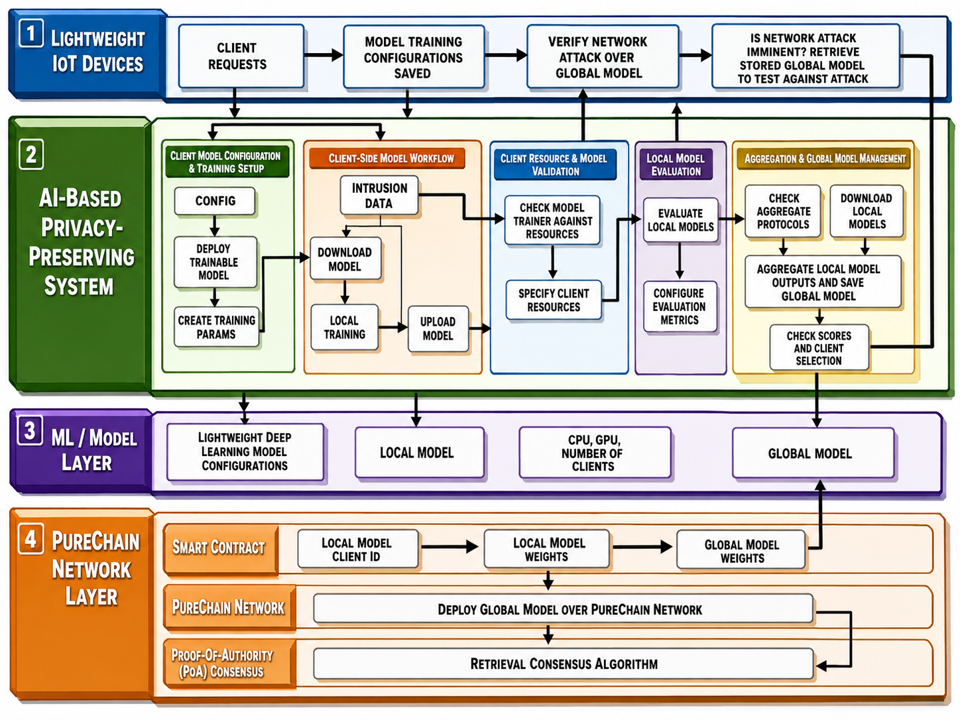
\includegraphics[width=\textwidth]{figures/Picture 16.png}
  \caption{Architecture of the behavioural trust-scoring stratum, recaptured from the published lightweight federated design~\cite{amadi2026lightweight}. Resource-constrained clients train a trimmed CNN--LSTM locally on their own telemetry; a coordinator aggregates the local updates into a global model by federated averaging; the resulting per-device trust scores are registered through the fast permissioned layer for commitment.}
  \label{fig:strata-fl-arch}
\end{figure}

\subsection{Detection Model}
\label{subsec:strata-model}
The engine pairs a one-dimensional convolutional front end with a recurrent stage. The convolutional layers act as a feature compressor over packet-flow statistics, capturing short-range structure such as burst rates and protocol flags, and the recurrent stage models the longer-range temporal dependence of an attack that unfolds across a session. A purely convolutional model captures local patterns but lacks temporal memory, while a standalone recurrent model is costlier on constrained hardware; the hybrid keeps inference light by letting the convolutional layers reduce dimensionality before the recurrent stage operates. The engine and its trust-threshold decision are shown in Figure~\ref{fig:strata-cnnlstm}: telemetry is compressed by the convolutional and pooling stage, the LSTM stage captures temporal dependence, and the softmax output yields the trust score $q_i$, which the threshold test $q_i < \delta$ turns into either a committed trust score on the fast permissioned layer or a revocation event raised to the identity plane.

\begin{figure}[t]
  \centering
  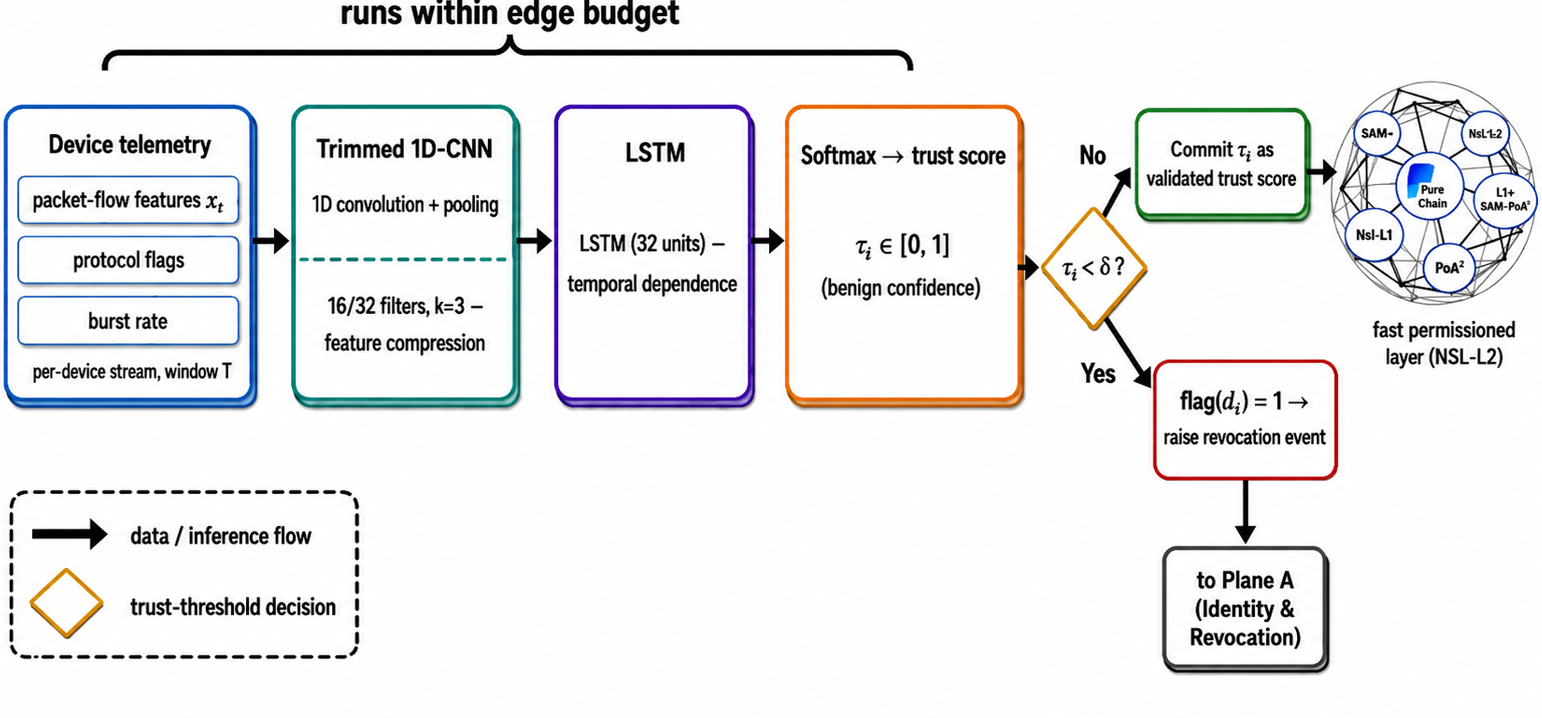
\includegraphics[width=\textwidth]{figures/Picture 15.PNG}
  \caption{Behavioural trust-scoring engine of Stratum~1. Device telemetry over a window $T$ passes through a trimmed one-dimensional CNN and pooling stage for feature compression, an LSTM stage for temporal dependence, and a softmax that yields the per-device trust score $q_i\in[0,1]$. The threshold test $q_i<\delta$ then either commits the score as a validated trust score to the fast permissioned layer or raises a revocation event to the identity plane.}
  \label{fig:strata-cnnlstm}
\end{figure}

For an input sequence $\mathbf{x} \in \mathbb{R}^{T \times d}$ of $d$-dimensional per-step feature vectors over a window of length $T$, the convolutional response of the $k$-th filter with kernel size $h$ is
\begin{equation}
\label{eq:strata-conv}
c_t^{(k)} \;=\; \mathrm{ReLU}\!\left( \sum_{i=0}^{h-1} \mathbf{w}_i^{(k)} \cdot \mathbf{x}_{t+i} + b^{(k)} \right),
\end{equation}
with same-length padding so boundary indices remain well defined. The pooled convolutional features pass to the LSTM stage, whose final hidden state $\mathbf{h}_T$ is mapped to a class distribution over the $C$ attack categories by
\begin{equation}
\label{eq:strata-softmax}
\hat{y}_j \;=\; \frac{\exp(z_j)}{\sum_{\ell=1}^{C} \exp(z_\ell)}, \qquad \mathbf{z} \;=\; \mathbf{W}_{\text{out}}\,\mathbf{h}_T + \mathbf{b}_{\text{out}}.
\end{equation}
The trust score of device $d_i$ is taken as the model's confidence in benign behaviour, $q_i \in [0,1]$, obtained from the benign component of $\hat{\mathbf{y}}$ under optional temperature calibration. This per-window score is the behavioural evidence that Plane~A accumulates into the device trust score $s_i$ of Equation~\eqref{eq:trust-decay}, so that a single anomalous window raises a flag without by itself withdrawing a credential. A device is flagged when its score falls below a predefined trust threshold $\delta$,
\begin{equation}
\label{eq:strata-flag}
\text{flag}(d_i) \;=\; \mathbf{1}\!\left[\, q_i < \delta \,\right],
\end{equation}
and a raised flag is the event that Plane~A carries into revocation and that Stratum~3 anchors as a proof. The threshold $\delta$ therefore sets the operating point at which behavioural drift becomes an accountable revocation, linking this stratum to the identity plane of Section~\ref{sec:strata-identity}.

\subsection{Federated Training and Commitment}
\label{subsec:strata-fedtrain}
Training keeps data local. Each client $i$ computes an update on its private telemetry and transmits only model weights to the coordinator, which forms the global model by federated averaging,
\begin{equation}
\label{eq:strata-fedavg}
\mathbf{w}^{(t+1)} \;=\; \sum_{i\in\mathcal{V}_t} \frac{n_i}{\sum_{j\in\mathcal{V}_t} n_j}\, \mathbf{w}_i^{(t)},
\end{equation}
where $n_i$ is the sample count at client $i$ and $\mathcal{V}_t$ is the set of registered clients whose updates are admitted in round $t$.
Weighting by local sample count reduces the instability that non-identical client distributions would otherwise introduce. Before a global update is accepted, its provenance is checked at the fast layer: only updates from registered clients, carrying a valid round identifier and timestamp, are admitted, which prevents model-poisoning through malformed or unregistered submissions. Algorithm~\ref{alg:strata-train} states the training and commitment procedure, and Figure~\ref{fig:strata-train-flow} shows the same procedure as an operational flow across its three phases, ending in the trust-scoring and flag step that produces the verdict this stratum commits. Training proceeds in rounds under a metadata-validated admission check, the finalised global model is committed through the fast-layer smart contract, and each device is then scored and either recorded as trusted or raised for revocation according to the threshold test of Equation~\eqref{eq:strata-flag}.

\begin{algorithm}[t]
\caption{Federated trust-model training and behavioural commitment}
\label{alg:strata-train}
\begin{algorithmic}[1]
\Require Clients $\{1,\ldots,K\}$, communication rounds $R$,
local epochs $E$, trust threshold $\delta$
\Ensure Global trust model $\mathbf{w}^{\star}$ and per-device flags
\State Initialise global model weights $\mathbf{w}^{(0)}$
\State Register client identities on the fast permissioned layer
\For{$t = 0$ to $R-1$}
    \ForAll{registered clients $i \in \{1,\ldots,K\}$ \textbf{in parallel}}
        \State $\mathbf{w}_{i}^{(t)}
        \gets
        \textsc{LocalTrain}\!\left(\mathbf{w}^{(t)},E\right)$
        using private telemetry
        \State Transmit $\mathbf{w}_{i}^{(t)}$ together with
        round ID and timestamp
    \EndFor
    \State $\mathcal{V}_{t}
    \gets
    \{\,i \mid i \text{ is registered and metadata is valid}\,\}$
    \State $\displaystyle
    \mathbf{w}^{(t+1)} \gets \sum_{i\in\mathcal{V}_t} \frac{n_i}{\sum_{j\in\mathcal{V}_t} n_j}\, \mathbf{w}_i^{(t)}$
    \Comment{Federated averaging, Eq.~\eqref{eq:strata-fedavg}}
\EndFor
\State $\mathbf{w}^{\star} \gets \mathbf{w}^{(R)}$
\State Commit $\mathbf{w}^{\star}$ through the fast-layer smart contract
\ForAll{devices $d_i$}
    \State $\hat{\mathbf{y}}_i
    \gets
    \mathcal{F}_{\mathbf{w}^{\star}}(\mathbf{x}_i)$
    \State $q_i
    \gets
    \textsc{BenignConfidence}(\hat{\mathbf{y}}_i)$
    \Comment{Eq.~\eqref{eq:strata-softmax}}
    \If{$q_i < \delta$}
        \State $\mathrm{flag}(d_i) \gets 1$
        \State Raise revocation event to Plane~A
        \Comment{Eq.~\eqref{eq:strata-flag}}
    \Else
        \State $\mathrm{flag}(d_i) \gets 0$
        \State Commit $q_i$ as a validated behavioural trust score
    \EndIf
\EndFor
\State \Return $\mathbf{w}^{\star}$ and per-device flags
\end{algorithmic}
\end{algorithm}

\begin{figure}[t]
  \centering
  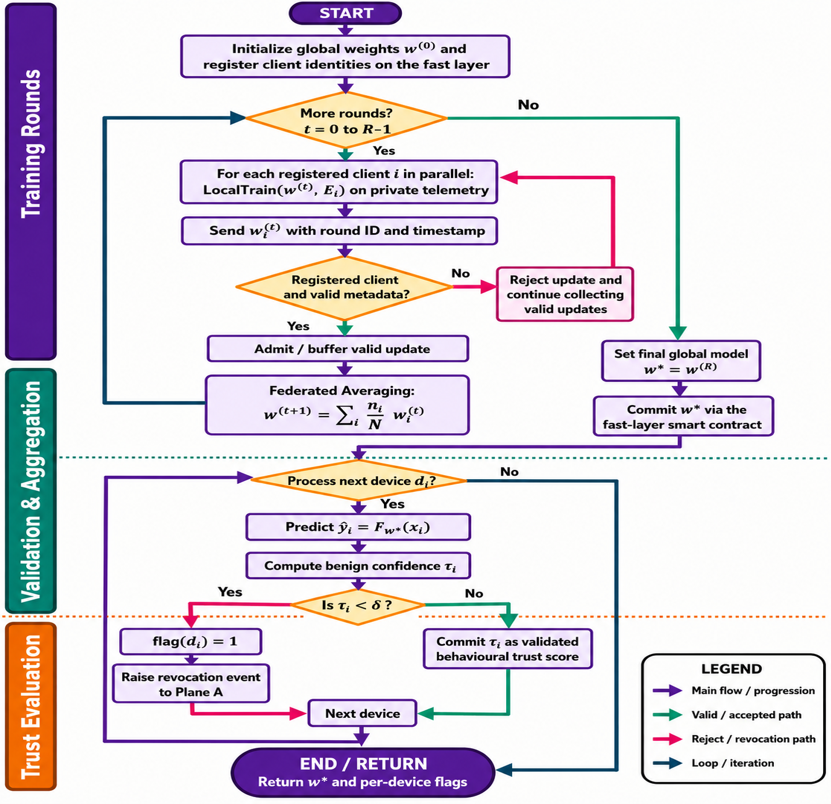
\includegraphics[width=\textwidth]{figures/Picture14.PNG}
  \caption{Operational flow of the federated trust-model training and behavioural commitment procedure.} 
  \label{fig:strata-train-flow}
\end{figure}

The trained engine is deliberately small, which is what allows continuous scoring within an edge budget. Its parameter count, layer configuration, and training settings are summarised in Table~\ref{tab:strata-hyper}, together with the trust threshold $\delta$ that fixes the flag rule of Equation~\eqref{eq:strata-flag}.

\begin{table}[t]
  \centering
  \footnotesize
  \setlength{\tabcolsep}{6pt}
  \renewcommand{\arraystretch}{1.25}
  \caption{Configuration of the trimmed CNN--LSTM trust engine and its trust-scoring rule. Model and training values are reused from the lightweight federated design; the final row states the trust-scoring output and flag threshold specific to this stratum.}
  \label{tab:strata-hyper}
  \begin{tabular}{@{}ll@{}}
    \toprule
    \textbf{Configuration item} & \textbf{Value} \\
    \midrule
    Model type              & 1-D CNN--LSTM \\
    Convolutional layers    & 16, 32 filters (kernel size 3) \\
    LSTM units              & 32 \\
    Dense layer             & 64 neurons + softmax output \\
    Activation              & ReLU (conv), softmax (output) \\
    Optimiser               & Adam \\
    Learning rate           & $1\times10^{-3}$ \\
    Batch size              & 64 \\
    Local epochs per round  & 5 \\
    Loss                    & categorical cross-entropy \\
    Dropout                 & 0.2 after the LSTM layer \\
    Trainable parameters    & 41{,}762 \\
    \addlinespace
    Trust score $q_i$    & benign-class confidence, $q_i\in[0,1]$ \\
    Flag rule               & $\text{flag}(d_i)=\mathbf{1}[q_i<\delta]$, threshold $\delta$ \\
    \bottomrule
  \end{tabular}
\end{table}
Kept to this size, the engine sustains continuous behavioural scoring on constrained hardware while producing a decision at the rate the fast layer requires. The verdict it commits is accurate but, once written, no longer alterable at the device, which is the property the next two strata build upon: Section~\ref{sec:strata-anchor} finalises and anchors these commitments, and Section~\ref{sec:strata-identity} converts a raised flag into an accountable revocation.


\section{The Consensus and Public-Anchoring Strata}
\label{sec:strata-anchor}

A behavioural verdict acquires no authority at the moment it is computed. Until it has been ordered against every other verdict in the network, accepted by a quorum that no single participant controls, and placed on a substrate that the accused device and its operator cannot rewrite, it remains a local opinion held by the gateway that produced it. The two upper strata of STRATA supply exactly those properties, and they supply them in sequence. The consensus and coordination stratum finalises the verdict inside the permissioned domain at a latency compatible with industrial control loops, and the public anchoring stratum carries a compact proof of that finalised record across the trust boundary onto a substrate whose write history lies beyond the reach of the consortium itself.

The division of labour is what keeps the arrangement affordable. Finalisation is frequent and cheap; anchoring is infrequent and expensive; assigning each class of event to the layer whose economics match its frequency is the operational content of trust-partitioning. Table~\ref{tab:strata-upper} sets the two strata against the properties each is required to deliver, and makes plain why neither could absorb the responsibilities of the other.

\begin{table}[t]
  \centering
  \footnotesize
  \setlength{\tabcolsep}{5pt}
  \renewcommand{\arraystretch}{1.3}
  \caption{Operational characteristics assigned to the consensus and public-anchoring strata, and the reason each property is unattainable on the other layer.}
  \label{tab:strata-upper}
  \begin{tabularx}{\textwidth}{@{}
      >{\raggedright\arraybackslash}p{2.9cm}
      >{\raggedright\arraybackslash}p{3.2cm}
      >{\raggedright\arraybackslash}p{3.2cm}
      >{\raggedright\arraybackslash}X@{}}
    \toprule
    \textbf{Property} & \textbf{Stratum~2 (consensus)} & \textbf{Stratum~3 (anchoring)} & \textbf{Reason for the split} \\
    \midrule
    Event frequency
      & Every behavioural verdict
      & One commitment per epoch
      & Per-event public writes are unaffordable at industrial verdict rates \\
    Settlement
      & Deterministic, final on commit
      & Probabilistic, subject to confirmation depth
      & Control actions cannot wait out a confirmation window \\
    Write authority
      & Consortium validators
      & Outside consortium administration
      & An operator-controlled ledger cannot attest to operator conduct \\
    Content exposed
      & Records and evidence bundles
      & Digests and hashed identifiers only
      & Payload disclosure would create a surface the deployment does not have today \\
    Cost driver
      & Signature verification per block
      & Transaction fee per commitment
      & Compute is elastic inside the plant; public fees are not \\
    \bottomrule
  \end{tabularx}
\end{table}

Figure~\ref{fig:strata-ecosystem} shows the five components that realise both strata and the paths along which records travel between them. Records enter at NSL-L2, where the behavioural stratum executes and where verdict digests are assembled. Ordering and acceptance occur at NSL-L1 under the PoA$^2$ acceptance rule, with SAM+ regulating the rate at which blocks are produced so that the permissioned chain neither starves under light industrial load nor saturates during an alarm storm. Only after a block is final does any material leave the permissioned domain, and what leaves is a digest, never a payload, which is the concrete enforcement of Theorem~\ref{thm:verifiability}.

\begin{figure}[t]
  \centering
  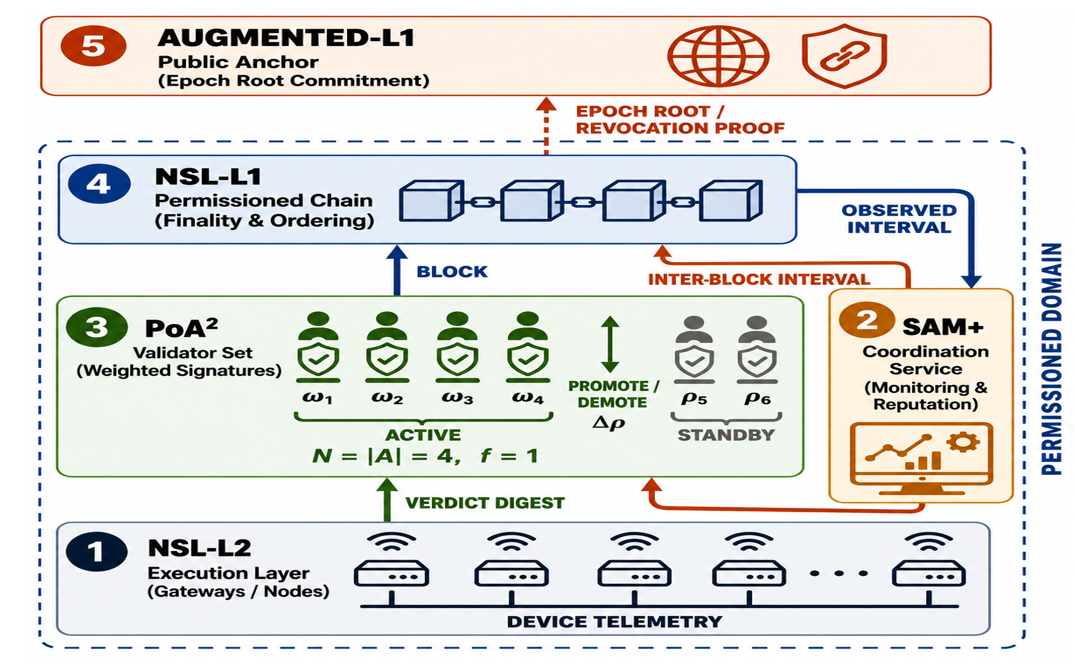
\includegraphics[width=\textwidth]{figures/Picture17.png}
  \caption{Component ecosystem realising the consensus and public-anchoring strata, comprising the SAM+ coordination service, the PoA$^2$ validator set, the NSL-L2 execution layer, the NSL-L1 permissioned chain, and the Augmented-L1 public anchor. Adapted from the published lightweight federated design~\cite{amadi2026lightweight}.}
  \label{fig:strata-ecosystem}
\end{figure}

\subsection{Consensus and Coordination}
\label{sec:strata-consensus}
Acceptance at the permissioned layer is decided by weighted authority rather than by expended work. Each validator $i$ in the active set $\mathcal{A}$ carries an authority weight $\omega_i$ that encodes both its institutional standing in the consortium and its observed operational reliability. A candidate block $B$ is committed when the weighted signatures it carries clear a fixed acceptance threshold:
\begin{equation}
\label{eq:poa2-accept}
\sum_{i \in \mathcal{A}} \omega_i \, \mathrm{sig}_i(B) \;\geq\; \theta ,
\end{equation}
where $\mathrm{sig}_i(B) \in \{0,1\}$ indicates whether validator $i$ signed $B$, $\omega_i \in [0,1]$ is the normalised authority weight of validator $i$, and $\theta$ is the acceptance threshold, set so that commitment requires a supermajority of weighted authority rather than a simple majority of nodes.

The reliability component of $\omega_i$ is not a static grant. It is tracked as an exponentially weighted moving average over the recent signing history of each validator, so that a node which is nominally authorised but persistently absent loses influence without requiring an administrative intervention:
\begin{equation}
\label{eq:poa2-reliability}
\rho_i(t) \;=\; \frac{\sum_{k=1}^{K} \gamma^{\,K-k} \, \mathrm{sig}_i(k)}{\sum_{k=1}^{K} \gamma^{\,K-k}} ,
\end{equation}
where $\rho_i(t) \in [0,1]$ is the reliability of validator $i$ at time $t$, $\mathrm{sig}_i(k)$ indicates whether validator $i$ signed block $k$, $K$ is the length of the observation window, and $\gamma \in (0,1)$ is the decay factor that weights recent participation above historical participation.

Reliability governs membership as well as influence. Validators whose reliability falls are demoted to the standby set $\mathcal{S}$, and standby nodes with sustained availability are promoted in their place. The exchange is triggered by a gap condition that prevents the active set from drifting into a state where a standby node is measurably more dependable than a serving one:
\begin{equation}
\label{eq:poa2-gap}
\max_{j \in \mathcal{S}} \rho_j(t) \;-\; \min_{i \in \mathcal{A}} \rho_i(t) \;<\; \Delta_\rho ,
\end{equation}
where $\mathcal{S}$ is the standby set, $\mathcal{A}$ is the active set, and $\Delta_\rho$ is the admissible reliability gap. When the condition is violated, the least reliable active validator is replaced by the most reliable standby validator, which gives the validator set a self-healing property without opening membership to unvetted participants.

Because authority is assigned rather than mined, agreement is deterministic and a committed block is final on commitment. There is no probabilistic settlement period during which a competing fork might displace an accepted verdict, and consequently no confirmation depth that industrial applications must wait out before acting on a revocation. The safety margin of the arrangement follows from the Byzantine bound applied to the active set:
\begin{equation}
\label{eq:poa2-fault}
f \;=\; \left\lfloor \frac{N-1}{2} \right\rfloor , \qquad N \;\geq\; 2f + 1 ,
\end{equation}
where $N = |\mathcal{A}|$ is the number of active validators and $f$ is the maximum number of simultaneously faulty or unavailable validators the layer tolerates while still admitting blocks. The bound is weaker than the $N \geq 3f+1$ requirement of open Byzantine agreement, and deliberately so. Validator identity is known and misbehaviour is attributable, which converts an anonymous adversary problem into an accountable one and permits the smaller quorum that constrained deployments can realistically staff.

Block production is regulated by the SAM+ coordination service, which adjusts the effort required to produce a block in response to observed network conditions rather than holding it at a fixed value. Industrial traffic is bursty by nature, and a fixed interval either wastes capacity during quiet periods or accumulates a backlog when an incident causes many gateways to report at once. The regulation objective is a bounded inter-block interval across both regimes:
\begin{equation}
\label{eq:sam-band}
T_{\min} \;\leq\; \bar{T}_{w} \;\leq\; T_{\max} ,
\end{equation}
where $\bar{T}_{w}$ is the mean inter-block interval observed over a sliding window $w$, and $T_{\min}$ and $T_{\max}$ bound the admissible interval. Holding the observed mean inside the band is what allows the behavioural stratum to treat finalisation latency as a bounded quantity when scheduling its own commitment step, and it is the property against which the layer is later measured. Table~\ref{tab:consensus-params} collects the parameters that govern the stratum, the constraint each one expresses, and the effect of moving it.

\begin{table}[t]
  \centering
  \footnotesize
  \setlength{\tabcolsep}{5pt}
  \renewcommand{\arraystretch}{1.3}
  \caption{Parameters governing the consensus and coordination stratum, with the constraint each expresses and the consequence of altering it.}
  \label{tab:consensus-params}
  \begin{tabularx}{\textwidth}{@{}
      >{\raggedright\arraybackslash}p{1.6cm}
      >{\raggedright\arraybackslash}p{4.0cm}
      >{\raggedright\arraybackslash}p{2.6cm}
      >{\raggedright\arraybackslash}X@{}}
    \toprule
    \textbf{Symbol} & \textbf{Quantity} & \textbf{Governs} & \textbf{Effect of increase} \\
    \midrule
    $\theta$
      & Weighted acceptance threshold
      & Block acceptance
      & Stronger safety, reduced liveness under validator absence \\
    $\gamma$
      & Reliability decay factor
      & Reliability tracking
      & Longer memory of past participation, slower demotion \\
    $\Delta_\rho$
      & Admissible reliability gap
      & Set membership
      & Fewer set changes, greater tolerance of degraded validators \\
    $N$
      & Active validator count
      & Fault tolerance
      & Higher fault tolerance, higher signature-verification cost per block \\
    $T_{\max}$
      & Upper bound on inter-block interval
      & Block cadence
      & Lower block overhead, higher worst-case finalisation latency \\
    \bottomrule
  \end{tabularx}
\end{table}

\subsection{Public Anchoring}
\label{sec:strata-public}
Everything described so far is internal to a consortium that the plant operator controls, and that control is precisely the residual risk. A permissioned ledger operated by the party whose conduct is under audit offers no protection against a coordinated rewrite by that party. The public anchoring stratum removes the possibility by committing periodic digests of the permissioned history to a substrate outside consortium administration, so that any retrospective alteration inside the consortium becomes detectable by comparison against a record the consortium cannot edit.

The public layer exposes a narrow interface, and the narrowness is deliberate. Admission binds an identifier to a credential commitment without disclosing the credential:
\begin{equation}
\label{eq:register}
\mathrm{Register}(\mathrm{id}) \;\longmapsto\; \big\langle \, H(\mathrm{id}), \; H(\mathrm{pk}), \; \mathrm{dom}, \; t_e \, \big\rangle ,
\end{equation}
where $H(\mathrm{id})$ is the digest of the device identifier, $H(\mathrm{pk})$ is the digest of the public credential issued at enrolment, $\mathrm{dom}$ names the permissioned domain that vouches for the device, and $t_e$ is the enrolment timestamp. A relying party already in possession of an identifier and credential can confirm admission by recomputing both digests; a party in possession of neither learns only that some device was admitted, which is what prevents the public record from becoming an inventory of the plant.

Withdrawal is the mirror of admission, and it is the one class of event that is never deferred. When the behavioural stratum drives a device trust score below the revocation threshold $\tau$, the finding is not merely recorded, it is published, because its purpose is to inform parties outside the consortium that the credential is no longer honoured:
\begin{equation}
\label{eq:revoke}
\mathrm{Revoke}(\mathrm{id}) \;\Longrightarrow\; \big\langle \, H(\mathrm{id}), \; H(\pi), \; t_r \, \big\rangle ,
\end{equation}
where $H(\pi)$ is the digest of the evidence bundle supporting the revocation and $t_r$ is the revocation timestamp. The evidence bundle itself remains inside the permissioned domain and is disclosed only to parties with cause. What becomes public is the fact of revocation together with a commitment binding it to evidence that cannot subsequently be substituted, so a later dispute cannot be settled by producing a more convenient bundle. Publication succeeds only for a revocation block that has already cleared the weighted acceptance threshold, which is the point at which the two strata meet:
\begin{equation}
\label{eq:publish-revocation}
\mathrm{publishRevocation}\big(H(\mathrm{id}), H(\pi)\big) \;=\;
\begin{cases}
\text{committed}, & \text{if } \displaystyle\sum_{i \in \mathcal{A}} \omega_i \, \mathrm{sig}_i(B_r) \geq \theta, \\[6pt]
\text{rejected}, & \text{otherwise},
\end{cases}
\end{equation}
where $B_r$ is the revocation block carrying the withdrawal tuple. No single gateway, and no single validator, can withdraw a device unilaterally, and equally no operator can suppress a revocation that the validator set has already accepted.
Routine verdicts are handled differently, because publishing each one at the rate industrial monitoring produces them would exhaust any realistic transaction budget. They are aggregated by epoch, and the epoch is the unit that makes the arrangement viable.

\begin{definition}[Anchoring epoch]
\label{def:epoch}
An anchoring epoch $\mathcal{E}_k$ is the ordered set of finalised verdict digests $\{H_1, H_2, \ldots, H_E\}$ produced at the permissioned layer between two successive public commitments, where $E = |\mathcal{E}_k|$ is the epoch span.
\end{definition}

The digests in an epoch are combined into a single value by binary hashing, and that value alone crosses the boundary:
\begin{equation}
\label{eq:merkle-root}
R_k \;=\; \mathrm{MerkleRoot}\!\left(H_1, H_2, \ldots, H_E\right) ,
\end{equation}
where $R_k$ is the epoch root committed publicly and $H_j$ is the digest of the $j$-th finalised record in the epoch. Membership of any individual record in the anchored epoch is subsequently demonstrable by supplying $\lceil \log_2 E \rceil$ sibling hashes, so selective verification of one device history never requires disclosure of, or access to, the remaining records in the epoch. The public commitment records the root together with the minimal metadata needed to locate and interpret it:
\begin{equation}
\label{eq:anchor-tuple}
\mathcal{C}_k \;=\; \big\langle \, k, \; R_k, \; \mathrm{dom}, \; v, \; t_k \, \big\rangle ,
\end{equation}
where $k$ identifies the epoch, $R_k$ is the epoch root, $\mathrm{dom}$ names the permissioned domain of origin, $v$ is the schema version under which the records were serialised, and $t_k$ is the commitment timestamp. No device identifier, no feature vector, and no trust score appears in the commitment, which is why anchoring adds no disclosure surface to a deployment.

Verification is a single comparison. An auditor holding a claimed record recomputes its digest, recomputes the root along the supplied Merkle path, and tests the result against the anchored value:
\begin{equation}
\label{eq:anchor-verify}
V \;=\; \mathbf{1}\!\left[\, \hat{R}_k \;=\; R_k^{\mathrm{chain}} \,\right] ,
\end{equation}
where $\hat{R}_k$ is the root recomputed from the record and its Merkle path, $R_k^{\mathrm{chain}}$ is the root read from the public commitment, and $V = 1$ certifies that the record is exactly the one the consortium finalised in epoch $k$. A single altered bit anywhere in the epoch produces $V = 0$, and the alteration is detectable by any party, including one with no standing inside the consortium.

Two parameters govern the cadence, and they pull against each other. The epoch closes on whichever of a count bound and a time bound is reached first:
\begin{equation}
\label{eq:epoch-close}
\Delta t_{\mathrm{anchor}} \;=\; \min\!\left( \frac{E}{\lambda}, \; T_{\mathrm{epoch}} \right) ,
\end{equation}
where $\lambda$ is the verdict arrival rate, $E$ is the epoch span, and $T_{\mathrm{epoch}}$ is the maximum tolerated interval of unanchored exposure. The time bound is what protects a quiet installation: without it, a plant producing few verdicts would leave its history unanchored for arbitrarily long simply because the count never filled. Figure~\ref{fig:strata-epoch} shows the resulting cadence, with routine verdicts accumulating toward an epoch boundary while a sub-threshold verdict leaves immediately by the revocation path. The economic argument for epoch-based anchoring is stated directly.
\begin{figure}[t]
  \centering
  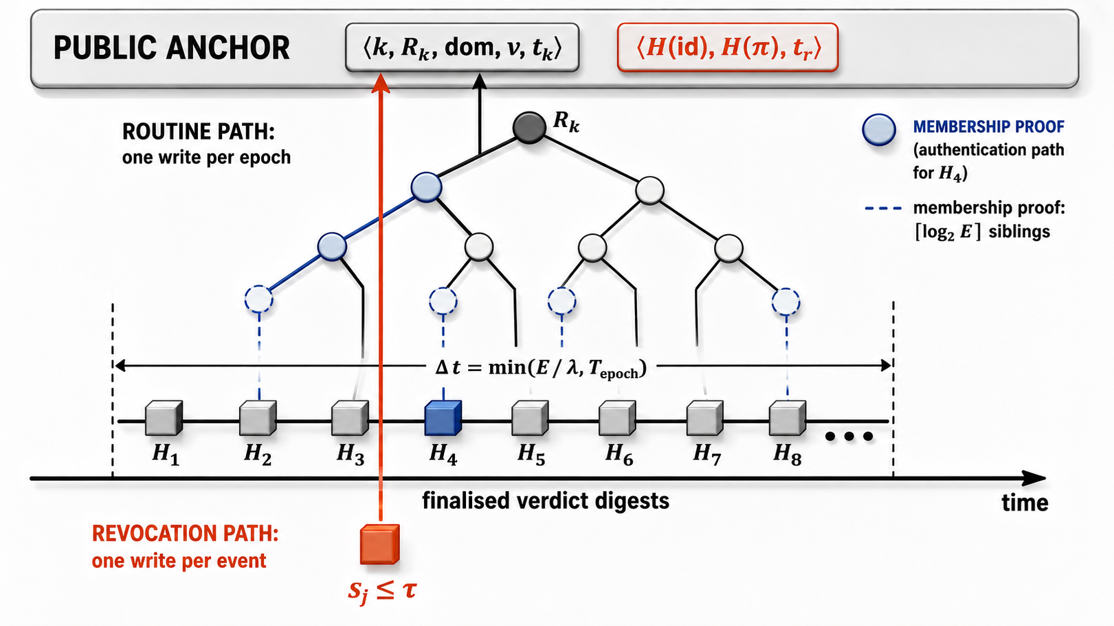
\includegraphics[width=\textwidth]{figures/Picture18.png}
  \caption{Anchoring cadence at the public stratum. Finalised verdict digests
accumulate across an epoch and are aggregated into a single root committed
once per epoch, while a verdict falling below the threshold $\tau$ is
published immediately by the revocation path and anchored in the epoch as
well.}
  \label{fig:strata-epoch}
\end{figure}



\begin{proposition}
\label{prop:anchor-rate}
For a verdict arrival rate $\lambda$ and an epoch span $E$, the public-layer write rate induced by routine anchoring is $\lambda / E$, and the evidence retained for any individual verdict is $\lceil \log_2 E \rceil$ hash values.
\end{proposition}

\begin{proof}
Each epoch consumes $E$ verdicts and produces exactly one commitment, so commitments are emitted at rate $\lambda / E$. Membership of a leaf in a balanced binary hash tree of $E$ leaves is witnessed by the sibling hash at each level, of which there are $\lceil \log_2 E \rceil$. Neither quantity depends on the size of the underlying record.
\end{proof}

The consequence is that public-layer cost is decoupled from behavioural event volume. Raising the epoch span reduces anchoring cost linearly while increasing proof size only logarithmically, and the operator tunes the span against the maximum acceptable interval of unanchored exposure rather than against a fixed transaction budget. Revocations are excluded from the aggregation and therefore from the reduction, which is the correct trade: the events that justify a per-event public write are exactly the events a relying party must learn about without waiting.
Table~\ref{tab:device-lifecycle} sets out the states a device occupies between admission and revocation, together with the transition that moves it and the stratum at which the transition is observed.

\begin{table}[t]
  \centering
  \footnotesize
  \setlength{\tabcolsep}{5pt}
  \renewcommand{\arraystretch}{1.3}
  \caption{Device lifecycle states, transition conditions, and the stratum at which each transition is observed.}
  \label{tab:device-lifecycle}
  \begin{tabularx}{\textwidth}{@{}
      >{\raggedright\arraybackslash}p{2.3cm}
      >{\raggedright\arraybackslash}X
      >{\raggedright\arraybackslash}p{3.6cm}
      >{\raggedright\arraybackslash}p{2.2cm}@{}}
    \toprule
    \textbf{State} & \textbf{Condition} & \textbf{Transition trigger} & \textbf{Observed at} \\
    \midrule
    Unregistered
      & No credential bound to the identifier
      & Enrolment and credential issue
      & Plane~A \\
    Active
      & Trust score above the operating band
      & Score falls into the monitored band
      & Stratum~1 \\
    Monitored
      & Score degraded but above $\tau$
      & Sustained degradation or a detection event
      & Stratum~1 \\
    Flagged
      & Score at or below $\tau$, pending finalisation
      & Revocation block reaches the acceptance threshold
      & Stratum~2 \\
    Revoked
      & Credential withdrawn and published
      & Terminal; re-entry requires re-enrolment
      & Stratum~3 \\
    \bottomrule
  \end{tabularx}
\end{table}

The lifecycle is monotone in one direction only. A device may recover from Monitored to Active while its score remains above $\tau$, but no transition returns a device from Revoked to Active, because the credential itself has been withdrawn and its replacement is a fresh enrolment producing a fresh identifier. The asymmetry is what makes a published revocation meaningful: a relying party observing the record on the public substrate does not have to establish whether the finding was later quietly reversed inside the consortium. Figure~\ref{fig:strata-crosschain} shows the crossing itself, from permissioned finalisation on one substrate to the commitment recorded on the other.

\begin{figure}[t]
  \centering
  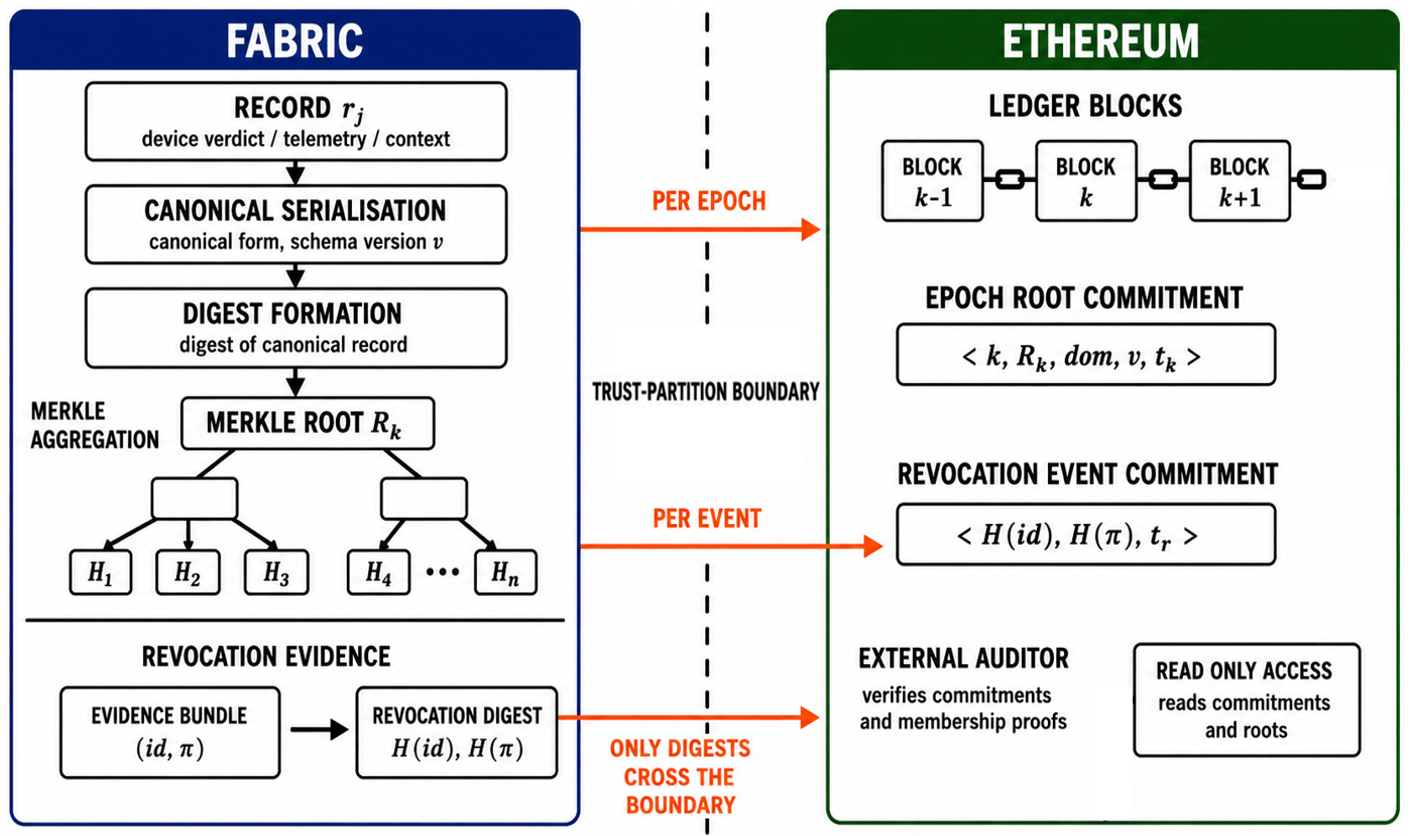
\includegraphics[width=0.92\textwidth]{figures/Picture19.PNG}
  \caption{Cross-boundary commitment path from the permissioned execution and consensus layers to the public anchor, showing digest formation, epoch aggregation, and the revocation channel. Adapted from the published hybrid-ledger cross-chain design~\cite{amadi2026symmetric}.}
  \label{fig:strata-crosschain}
\end{figure}

Algorithm~\ref{alg:strata-anchor} states the production procedure. It accepts the finalised verdict digests that the behavioural stratum produces, aggregates them by epoch, and diverts any record carrying a sub-threshold trust score into the revocation channel rather than the aggregation channel.

\begin{algorithm}[t]
\caption{Epoch anchoring and revocation-proof commitment}
\label{alg:strata-anchor}
\begin{algorithmic}[1]
\Require Stream of finalised records $\{r_j\}$ with trust scores $s_j$; epoch span $E$; epoch timeout $T_{\mathrm{epoch}}$; revocation threshold $\tau$; acceptance threshold $\theta$
\Ensure Public commitments $\{\mathcal{C}_k\}$ and published revocation records
\State $\mathcal{E} \gets \emptyset$; \; $k \gets 0$; \; start epoch timer
\For{each finalised record $r_j$ arriving from Stratum~2}
  \State $H_j \gets H(\mathrm{canonical}(r_j))$
  \If{$s_j \leq \tau$}
    \State $\pi_j \gets$ evidence bundle for $r_j$, retained in the permissioned domain
    \State assemble revocation block $B_r$ carrying $\langle H(\mathrm{id}_j), H(\pi_j), t_r \rangle$
    \If{$\sum_{i \in \mathcal{A}} \omega_i \, \mathrm{sig}_i(B_r) \geq \theta$}
      \State publish the tuple to the public anchor
      \State set lifecycle state of $\mathrm{id}_j$ to Revoked
    \EndIf
  \EndIf
  \State $\mathcal{E} \gets \mathcal{E} \cup \{H_j\}$
  \If{$|\mathcal{E}| = E$ \textbf{or} epoch timer $\geq T_{\mathrm{epoch}}$}
    \State $R_k \gets \mathrm{MerkleRoot}(\mathcal{E})$
    \State commit $\mathcal{C}_k \gets \langle k, R_k, \mathrm{dom}, v, t_k \rangle$ to the public anchor
    \State retain Merkle paths for the members of $\mathcal{E}$ in the permissioned domain
    \State $\mathcal{E} \gets \emptyset$; \; $k \gets k+1$; \; reset epoch timer
  \EndIf
\EndFor
\State \Return $\{\mathcal{C}_k\}$ and the published revocation records
\end{algorithmic}
\end{algorithm}

The audit procedure that consumes those commitments is stated separately in Algorithm~\ref{alg:strata-verify}, because the party that runs it is not the party that produced the record. An auditor requires the record under examination, the Merkle path retained beside it, and read access to the public substrate. No credential, no consortium membership, and no cooperation from the operator beyond release of the record is needed, which is the property that distinguishes anchoring from internal logging.

\begin{algorithm}[t]
\caption{Independent verification of an anchored record}
\label{alg:strata-verify}
\begin{algorithmic}[1]
\Require Claimed record $r$; Merkle path $\Pi$; epoch index $k$; read access to the public anchor
\Ensure Verdict $V \in \{0,1\}$ on the integrity of $r$
\State $\hat{H} \gets H(\mathrm{canonical}(r))$ \Comment{same serialisation rules and schema version $v$}
\State $\hat{R}_k \gets \hat{H}$
\For{each sibling $h \in \Pi$, from leaf to root}
  \State $\hat{R}_k \gets H(\hat{R}_k \,\|\, h)$ in the order recorded by the path
\EndFor
\State read $\mathcal{C}_k = \langle k, R_k^{\mathrm{chain}}, \mathrm{dom}, v, t_k \rangle$ from the public anchor
\If{schema version of $r$ $\neq v$}
  \State \Return $V \gets 0$ \Comment{serialisation mismatch invalidates the comparison}
\EndIf
\State $V \gets \mathbf{1}[\hat{R}_k = R_k^{\mathrm{chain}}]$
\State \Return $V$
\end{algorithmic}
\end{algorithm}

Two properties of the pair deserve emphasis, because they are the properties an evaluator will test. First, the public substrate receives no data whose disclosure could harm the operator: the aggregation channel emits roots, and the revocation channel emits hashed identifiers and evidence commitments, so the anchoring stratum adds durability without adding exposure. Second, the cost the operator pays for that durability is bounded and tunable by a single parameter, the routine public write rate holding at $\lambda/E$ independent of how much behavioural traffic the lower strata process. The measured expression of both properties, in anchoring latency and in per-device overhead on constrained hardware, is reported in Chapter~\ref{Chapter_5}.

What remains unspecified is the credential that binds a device to the identifier carried in the registration and withdrawal records, the law by which a trust score decays toward the threshold that triggers withdrawal, and the cryptographic substrate that must keep credential and anchored commitment meaningful once classical hardness assumptions no longer hold. Those are the concerns of the two cross-cutting planes, treated in Section~\ref{sec:strata-identity}.


\section{Quantum-Resilient Identity and Revocation}
\label{sec:strata-identity}

The three strata described so far assume two things they do not themselves provide. Every record carries a device identifier, and the whole apparatus of behavioural scoring, finalisation and anchoring is worthless if that identifier can be forged, cloned across devices, or reused after withdrawal. Every digest, signature and key exchange rests on a hardness assumption, and a deployment expected to remain in service for fifteen years cannot assume that the assumption holding today still holds at decommissioning. Neither concern belongs to a single stratum. Identity is asserted at the edge, evaluated at the behavioural layer, finalised at the consensus layer and published at the anchor; cryptographic strength is required at each of those points and at the boundaries between them. Both are therefore carried as planes cutting vertically through the stack rather than as layers stacked upon it.

Plane~A binds a physical device to an identifier and governs the withdrawal of that binding. Plane~B supplies the cryptographic substrate on which the binding, and every commitment derived from it, is expressed. Table~\ref{tab:planes-matrix} states what each plane contributes at each stratum, and the pattern in the table is the justification for treating them as planes: no row is empty, and no stratum could supply for itself what the planes supply.

\begin{table}[t]
  \centering
  \footnotesize
  \setlength{\tabcolsep}{5pt}
  \renewcommand{\arraystretch}{1.3}
  \caption{Contribution of the two cross-cutting planes at each stratum of the architecture.}
  \label{tab:planes-matrix}
  \begin{tabularx}{\textwidth}{@{}
      >{\raggedright\arraybackslash}p{3.0cm}
      >{\raggedright\arraybackslash}X
      >{\raggedright\arraybackslash}X@{}}
    \toprule
    \textbf{Stratum} & \textbf{Plane~A: identity and revocation} & \textbf{Plane~B: post-quantum substrate} \\
    \midrule
    Behavioural trust
      & Supplies the identifier under which observations are attributed and scores accumulated
      & Protects model updates in transit between gateway and aggregator \\
    Consensus and coordination
      & Supplies the credential a validator checks before admitting a record for ordering
      & Protects the session keys under which validators exchange candidate blocks \\
    Public anchoring
      & Supplies the hashed identifier published on withdrawal, and the evidence commitment bound to it
      & Determines how long an anchored commitment remains meaningful against a future adversary \\
    \bottomrule
  \end{tabularx}
\end{table}

\subsection{Plane A: Identity Derivation and Trust Decay}
\label{sec:plane-a}

An identifier that is assigned administratively can be reassigned administratively, which places the operator inside the trust boundary of every claim made about a device. Deriving the identifier from physical entropy captured at the device removes that discretion. The identifier is fixed at enrolment as the digest of three concatenated components:
\begin{equation}
\label{eq:identity-derive}
\mathrm{id}_i \;=\; H\big( e_i \,\|\, t_i \,\|\, d_i \big) ,
\end{equation}
where $e_i$ is a sample drawn from the device entropy source, $t_i$ is the enrolment timestamp, and $d_i$ is a device-specific token held in the secure element. The entropy sample makes the identifier unpredictable to an adversary who knows the device model and enrolment time; the timestamp makes a replayed enrolment produce a distinct identifier; and the device token binds the result to hardware that cannot be relocated without physical access. None of the three is sufficient alone, and the digest is one-way, so publishing the identifier discloses nothing about the entropy sample that produced it.

\begin{definition}[Device credential]
\label{def:credential}
A device credential is the pair $\langle \mathrm{id}_i, \mathrm{pk}_i \rangle$ formed at enrolment, where $\mathrm{id}_i$ is derived from device entropy and $\mathrm{pk}_i$ is the public key of the keypair generated in the secure element. The credential is valid while the trust score of the device remains above the revocation threshold, and terminally invalid thereafter.
\end{definition}

Table~\ref{tab:entropy-sources} lists the sources available on constrained industrial hardware, distinguishing what a given class of device can actually offer from what the derivation requires of it.

\begin{table}[t]
  \centering
  \footnotesize
  \setlength{\tabcolsep}{5pt}
  \renewcommand{\arraystretch}{1.3}
  \caption{Entropy sources available for identifier derivation on constrained industrial hardware.}
  \label{tab:entropy-sources}
  \begin{tabularx}{\textwidth}{@{}
      >{\raggedright\arraybackslash}p{2.8cm}
      >{\raggedright\arraybackslash}p{2.2cm}
      >{\raggedright\arraybackslash}p{3.4cm}
      >{\raggedright\arraybackslash}X@{}}
    \toprule
    \textbf{Source} & \textbf{Class} & \textbf{Availability} & \textbf{Suitability for one-time derivation} \\
    \midrule
    Hardware TRNG in secure element
      & Physical
      & Security-class microcontrollers; absent from legacy field devices
      & Preferred wherever present; no debiasing or conditioning required \\
    Ring-oscillator jitter
      & Physical
      & FPGA and selected microcontroller families
      & Throughput well above what a single enrolment consumes \\
    SRAM power-up state
      & Physical
      & Any device exposing uninitialised SRAM
      & One sample per power cycle; device-unique but requires debiasing \\
    Sensor noise floor
      & Environmental
      & Universal on instrumented devices
      & Serviceable fallback; entropy rate varies with process conditions \\
    Seeded software generator
      & Simulated
      & Any platform
      & Architectural validation only; unsuitable for a fielded credential \\
    \bottomrule
  \end{tabularx}
  \vspace{2pt}
  \footnotesize\raggedright
  Identifier derivation in the present realisation is seeded from the software source in the final row. The four physical and environmental sources are specified as deployment options and are not exercised here.
\end{table}

The construction consumes the entropy sample as an opaque bit string, so substituting a hardware source at deployment changes the quality of that sample and nothing else: the derivation, the storage cost of the resulting identifier, and every subsequent lifecycle operation are unaffected. What the present realisation establishes is that those operations behave as specified end to end; what it leaves to a fielded deployment is the entropy quality the chosen source actually delivers.

Withdrawal is driven by accumulated behavioural evidence rather than by a single detection. The trust score of a device is updated once per observation window by blending its previous value with the evidence from the current window:
\begin{equation}
\label{eq:trust-decay}
s_i(t+1) \;=\; \beta \, s_i(t) \;+\; (1-\beta) \, q_i(t) ,
\end{equation}
where $s_i(t) \in [0,1]$ is the trust score of device $i$ at window $t$, $q_i(t) \in [0,1]$ is the behavioural evidence produced for that window by the trust-scoring stratum, and $\beta \in (0,1)$ is the retention factor governing how strongly past behaviour resists present evidence. A high retention factor makes the score slow to fall, which suppresses reaction to transient noise at the cost of delaying response to a genuine compromise; a low factor inverts both properties. Withdrawal follows once the score falls to or below the revocation threshold $\tau$, at which point the credential is terminally invalid. Because the update is a convex combination, the score cannot leave the unit interval, and a device supplying uniformly clean evidence converges upward toward unity rather than accumulating unbounded credit for good behaviour.

A second, independent trigger bounds the response to abrupt compromise. A streak counter $S_i(t)$ records the number of consecutive windows in which the behavioural score $q_i(t)$ has fallen below the flag threshold $\delta$, and is reset by any window of normal behaviour. Withdrawal therefore follows when either condition is met,
\begin{equation}
\label{eq:revoke-condition}
\mathrm{Revoke}(\mathrm{id}_i) \iff s_i(t) \leq \tau \;\; \text{or} \;\; S_i(t) > \mu_S ,
\end{equation}
where $\mu_S$ is the streak limit. The threshold condition catches gradual degradation accumulated over many windows, while the streak condition catches a device that fails every window in succession before its score has had time to fall. The trust law may equally be realised in an additive form, in which each window credits or penalises the score by a fixed amount; that form shares the threshold semantics and the terminal withdrawal of Equation~\eqref{eq:trust-decay} but declines linearly rather than geometrically, and it is the form exercised in the isolation experiments of Chapter~\ref{Chapter_5}.

The delay this introduces between compromise and withdrawal is bounded, and the bound is what an operator needs in order to choose the retention factor.

\begin{proposition}
\label{prop:revocation-delay}
Let a device hold score $s_i(0) > \tau$ and thereafter supply evidence at a constant level $q < \tau$. The number of observation windows before withdrawal is
\[
k \;=\; \left\lceil \frac{\ln\!\big( (\tau - q) / (s_i(0) - q) \big)}{\ln \beta} \right\rceil .
\]
\end{proposition}

\begin{proof}
Writing the update as a deviation from the evidence level, $s_i(t+1) - q = \beta\,(s_i(t) - q)$, so $s_i(k) - q = \beta^{k}\,(s_i(0) - q)$. Withdrawal occurs at the least $k$ satisfying $s_i(k) \leq \tau$, that is $\beta^{k}(s_i(0) - q) \leq \tau - q$. Both sides are positive because $q < \tau < s_i(0)$, and $\ln \beta < 0$, so taking logarithms and dividing reverses the inequality and yields the stated expression on rounding up to a whole window.
\end{proof}

Two consequences follow. The first is a design guide: an operator who fixes an acceptable response time can solve the expression for the retention factor rather than tuning it by trial. The second is a limitation. Time to withdrawal grows without bound as the evidence level approaches the threshold from below, so an adversary degrading behaviour just far enough to sit marginally beneath it is withdrawn slowly. That strategy is defeated by detecting the degradation, not by accelerating the decay, since a decay steep enough to catch it would withdraw healthy devices on transient noise. The score is a filter over evidence rather than a detector in its own right, and responsibility for recognising the pattern sits with the behavioural stratum. Figure~\ref{fig:trust-decay} places the scoring loop in the wider credential lifecycle it governs.

\begin{figure}[t]
  \centering
  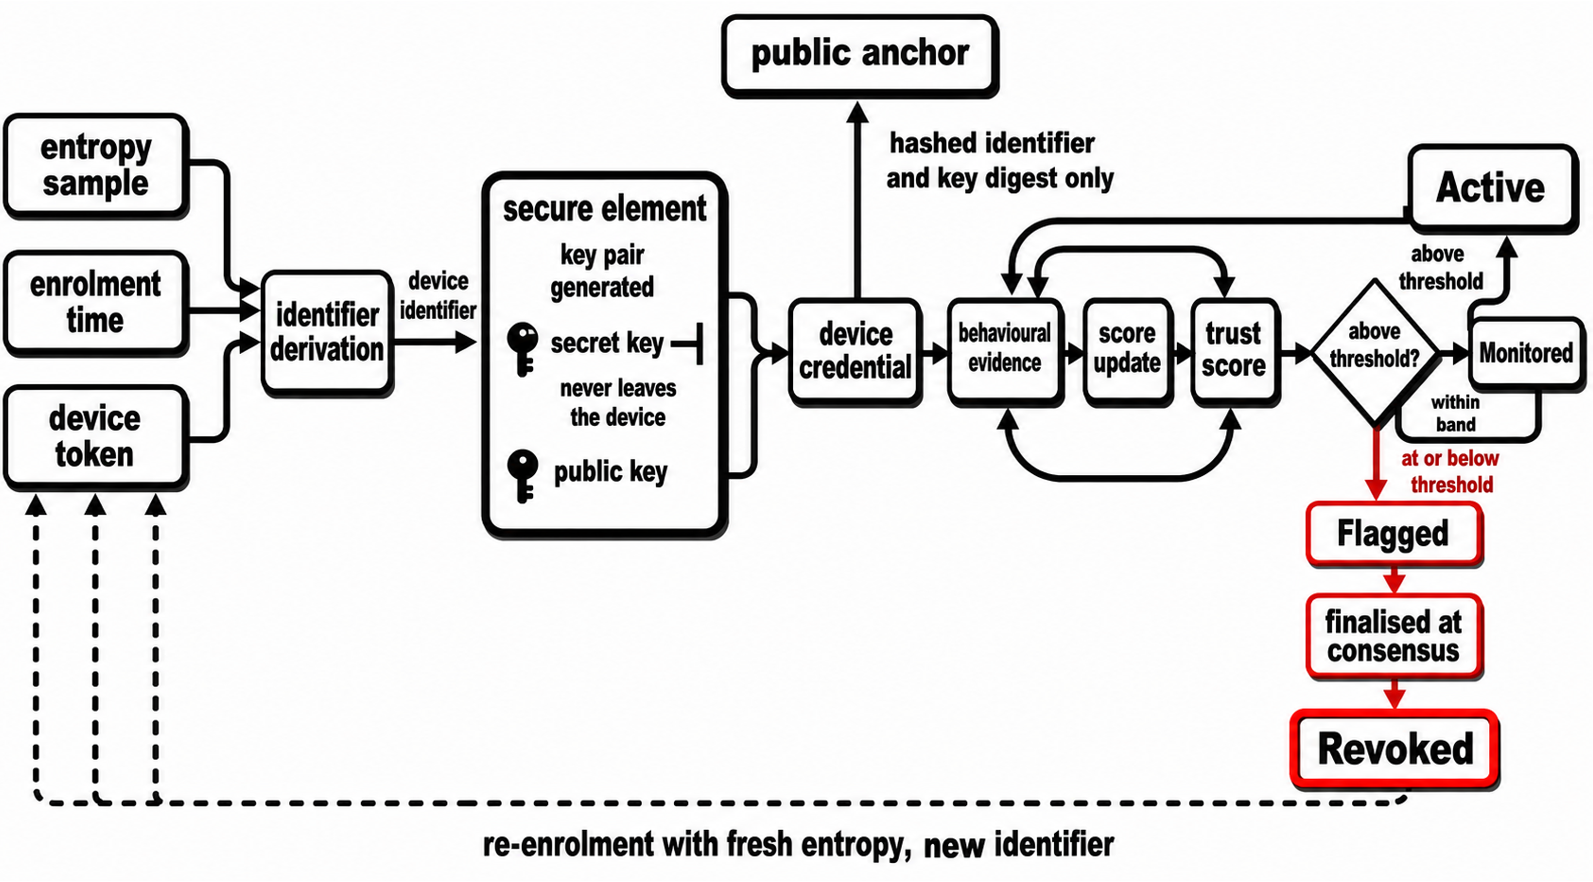
\includegraphics[width=\textwidth]{figures/Picture20.PNG}
  \caption{Credential mechanism of Plane~A, from entropy-seeded derivation and secure-element binding through the scoring loop to withdrawal. Withdrawal is terminal, and replacement requires re-enrolment under a fresh identifier.}
  \label{fig:trust-decay}
\end{figure}

Algorithm~\ref{alg:identity-lifecycle} sets out the full credential lifecycle, from enrolment through scoring to withdrawal and the handling of a replacement device.

\begin{algorithm}[t]
\caption{Credential issuance, decay and withdrawal}
\label{alg:identity-lifecycle}
\begin{algorithmic}[1]
\Require Device $i$ presenting entropy sample $e_i$ and device token $d_i$; retention factor $\beta$; revocation threshold $\tau$; initial score $s_0$
\Ensure Credential $\langle \mathrm{id}_i, \mathrm{pk}_i \rangle$ and its lifecycle state
\State $\mathrm{id}_i \gets H(e_i \,\|\, t_i \,\|\, d_i)$
\State generate keypair $(\mathrm{sk}_i, \mathrm{pk}_i)$ inside the secure element; $\mathrm{sk}_i$ never leaves it
\State register $\langle H(\mathrm{id}_i), H(\mathrm{pk}_i), \mathrm{dom}, t_i \rangle$ at the public anchor
\State $s_i \gets s_0$; \; state $\gets$ Active
\For{each observation window $t$}
  \State $q_i(t) \gets$ behavioural evidence from the trust-scoring stratum
  \State $s_i \gets \beta \, s_i + (1-\beta)\, q_i(t)$
  \State update streak counter $S_i$ \Comment{reset on a normal window}
  \If{$s_i \leq \tau$ \textbf{or} $S_i > \mu_S$}
    \State state $\gets$ Flagged; assemble evidence bundle $\pi_i$
    \State submit revocation for finalisation at the consensus stratum
    \If{revocation is committed}
      \State publish $\langle H(\mathrm{id}_i), H(\pi_i), t_r \rangle$; \; state $\gets$ Revoked
      \State \textbf{break} \Comment{terminal; the credential is not reinstated}
    \EndIf
  \ElsIf{$s_i$ below the operating band}
    \State state $\gets$ Monitored
  \Else
    \State state $\gets$ Active
  \EndIf
\EndFor
\State \Return $\langle \mathrm{id}_i, \mathrm{pk}_i \rangle$, state
\end{algorithmic}
\end{algorithm}

Replacement of a withdrawn device re-enters the procedure at the first line with a fresh entropy sample, producing an identifier unrelated to the withdrawn one. There is no reinstatement path, and there is no derivation linking the replacement to its predecessor, so an adversary observing the public record cannot establish that a newly admitted device occupies the position of a recently withdrawn one.

\subsection{Plane B: Post-Quantum Substrate}
\label{sec:plane-b}
A commitment anchored today is intended to remain checkable for the service life of the installation, and an industrial asset outlives several cryptographic generations. Two distinct exposures follow, and they have different urgencies. Confidentiality is exposed retroactively, because traffic captured now can be stored and decrypted once a capable adversary exists, so key establishment must be migrated before such an adversary appears rather than after. Integrity is exposed prospectively: a digest cannot be retrospectively forged into a commitment already published, so anchored records are threatened only from the point at which forgery becomes feasible.

Key establishment therefore adopts a lattice-based encapsulation mechanism in place of classical key agreement. The sender encapsulates against the recipient public key, obtaining a ciphertext to transmit and a shared secret to retain; the recipient recovers the same secret by decapsulating that ciphertext with the secret key held in its secure element. The shared secret never traverses the network in any form, and the ciphertext discloses nothing about it to an observer lacking the secret key.

The obstacle to deploying this on constrained hardware is size rather than speed. Lattice ciphertexts and public keys are substantially larger than their elliptic-curve counterparts, and on low-rate industrial radio links the transmission cost of that expansion dominates the computational cost of the primitive itself. A reversible compression is therefore applied to the ciphertext before transmission and inverted on receipt. The map is lossless with respect to the decapsulation input, so the shared secret recovered after inversion is identical to the one that would have been recovered from the uncompressed ciphertext, and the security argument for the underlying mechanism is unaffected. The reduction achieved and its effect on end-to-end handshake latency on constrained hardware are reported in Chapter~\ref{Chapter_5}.

Table~\ref{tab:pq-placement} records where each primitive sits in the architecture and which exposure it answers, together with the migration status of each position.

\begin{table}[t]
  \centering
  \footnotesize
  \setlength{\tabcolsep}{5pt}
  \renewcommand{\arraystretch}{1.3}
  \caption{Placement of cryptographic primitives across the architecture, the exposure each position carries, and its migration status in the present design.}
  \label{tab:pq-placement}
  \begin{tabularx}{\textwidth}{@{}
      >{\raggedright\arraybackslash}p{3.4cm}
      >{\raggedright\arraybackslash}p{2.9cm}
      >{\raggedright\arraybackslash}X
      >{\raggedright\arraybackslash}p{2.3cm}@{}}
    \toprule
    \textbf{Position} & \textbf{Primitive class} & \textbf{Exposure} & \textbf{Status} \\
    \midrule
    Device-to-gateway session
      & Lattice encapsulation
      & Retroactive: captured traffic decrypted later
      & Migrated \\
    Gateway-to-aggregator update transfer
      & Lattice encapsulation
      & Retroactive: model updates disclose local behaviour
      & Migrated \\
    Identifier derivation
      & Hash
      & Preimage resistance degrades by a square-root factor only
      & Adequate \\
    Record and epoch digests
      & Hash
      & Collision resistance sets the forgery horizon for anchored records
      & Adequate \\
    Validator block signatures
      & Digital signature
      & Prospective: forgery feasible only once a capable adversary exists
      & Migration item \\
    Device credential signatures
      & Digital signature
      & Prospective: forged credentials admit unauthorised devices
      & Migration item \\
    \bottomrule
  \end{tabularx}
\end{table}

Two rows of that table are marked as outstanding, and the reason is worth stating rather than leaving to inference. Signature migration multiplies key and signature sizes at every point where a block is signed and every point where a credential is presented, and unlike the session case those artefacts are stored rather than transmitted once. Sizing that cost against the storage budget of a field gateway is an engineering exercise the present design has not completed, and the prospective nature of the exposure makes deferral defensible in a way that deferring key establishment would not be. The hash positions carry no migration item because the known quantum advantage against preimage resistance is quadratic rather than exponential, which is absorbed by the digest lengths already in use.

\section{Cross-Substrate Instantiation and Setup}
\label{sec:strata-substrates}

An architecture demonstrated on one ledger and nowhere else invites a reasonable objection: that what has been shown is a property of that ledger rather than of the design built upon it. The objection is not academic. Permissioned and public substrates differ in their execution model, their finality semantics, their transaction economics and their identity assumptions, and a partition that survives only under one particular combination of those properties is an implementation detail dressed as a principle. Establishing that trust-partitioning is a property of the design requires realising the same partition twice, on substrates chosen for their difference rather than their similarity, and showing that the roles assigned to each stratum are discharged in both.

Two instantiations are used. The first realises all three strata on a purpose-built lightweight ledger with a native two-layer execution model, an authority-weighted consensus and a public anchor of its own. The second realises the identical partition on an enterprise pairing in which a permissioned chain provides execution and finalisation and a general-purpose public chain provides anchoring. The substrates were not chosen for convenience: one is a research ledger designed for constrained devices, the other a production stack with an installed base in industrial consortia, and their consensus mechanisms, block cadences and cost models have almost nothing in common. That distance is what gives the comparison its force.

\begin{definition}
\label{def:faithful-instantiation}
An instantiation of the architecture on a given substrate pair is faithful when four conditions hold: behavioural scoring executes on a layer whose write cost permits per-observation commitment; finalisation is decided by a bounded, identified validator set rather than by open participation; the material crossing the trust boundary consists of digests and hashed identifiers only; and withdrawal of a credential is published on the public side without disclosing the evidence that justified it.
\end{definition}

Faithfulness is what the two instantiations are required to demonstrate, and it is deliberately stated in terms of roles rather than mechanisms. Nothing in the four conditions names a consensus algorithm, a block interval or a ledger. A substrate satisfies them by whatever means it has available, which is precisely the claim under test: that the partition is specified at the level of trust roles and is therefore portable across the mechanisms that discharge them.

Table~\ref{tab:substrate-mapping} sets the two instantiations against each other role by role. Reading it by row rather than by column is what makes the point: each row states a responsibility, and the two entries beside it are different means to the same end.

\begin{table}[tb]
  \centering
  \footnotesize
  \setlength{\tabcolsep}{5pt}
  \renewcommand{\arraystretch}{1.3}
  \caption{Assignment of architectural roles to substrate components in the two instantiations.}
  \label{tab:substrate-mapping}
  \begin{tabularx}{\textwidth}{@{}
      >{\raggedright\arraybackslash}p{3.2cm}
      >{\raggedright\arraybackslash}X
      >{\raggedright\arraybackslash}X@{}}
    \toprule
    \textbf{Role} & \textbf{Instantiation~I: PureChain NSL} & \textbf{Instantiation~II: Fabric with Ethereum} \\
    \midrule
    Behavioural execution
      & Native fast execution layer, committing one record per observation window
      & Permissioned chaincode invoked per observation window \\
    Ordering and finality
      & Authority-weighted consensus with adaptive block cadence, final on commit
      & Raft ordering service under an endorsement policy, final on commit \\
    Validator identity
      & Consortium validators with authority weights and reliability tracking
      & Organisation-scoped identities issued by a membership service \\
    Public anchoring
      & PureChain public anchor receiving epoch roots
      & Ethereum receiving epoch roots by contract call, under a confirmation depth of three \\
    Credential registration
      & Anchor contract holding hashed identifier and key digest
      & Anchor contract holding hashed identifier and key digest \\
    Revocation publication
      & Per-event commitment on the public anchor
      & Per-event contract call on the public chain \\
    Cost model
      & Zero-fee operation throughout
      & Zero-fee on the permissioned side, fee-bearing on the public side \\
    \bottomrule
  \end{tabularx}
\end{table}

The final row is where the two instantiations diverge most sharply, and it is the row that matters most for deployment. Anchoring on a fee-bearing public chain converts the epoch span from a tuning parameter into a budget decision, since every commitment carries a direct cost, whereas anchoring on a zero-fee chain makes the same parameter a question of storage and audit latency alone. Combining the bounded write rate established for the anchoring stratum with a per-commitment fee gives the anchoring cost per unit time on a fee-bearing substrate:
\begin{equation}
\label{eq:anchor-cost}
C \;=\; \frac{\lambda}{E} \, c_{\mathrm{tx}} \;+\; \lambda_r \, c_{\mathrm{tx}} ,
\end{equation}
where $\lambda$ is the verdict arrival rate, $E$ is the epoch span, $c_{\mathrm{tx}}$ is the fee for a single commitment, and $\lambda_r$ is the revocation rate. The first term is compressible by raising the epoch span and the second is not, since revocations are published per event, so the floor on anchoring cost is set by how often devices are withdrawn rather than by how much behavioural traffic the installation generates. An operator with a fixed anchoring budget can therefore solve for the epoch span that meets it, subject to the exposure bound that governs how long the permissioned history may remain unanchored. On the zero-fee instantiation both terms vanish and the span is chosen on audit latency alone, which is why the same architecture admits very different operating points on the two substrates.

Figure~\ref{fig:substrate-instantiation} places the two instantiations side by side, with the role labels held constant across both panels so that substitution of the underlying components is visible at a glance.

\begin{figure}[tb]
  \centering
  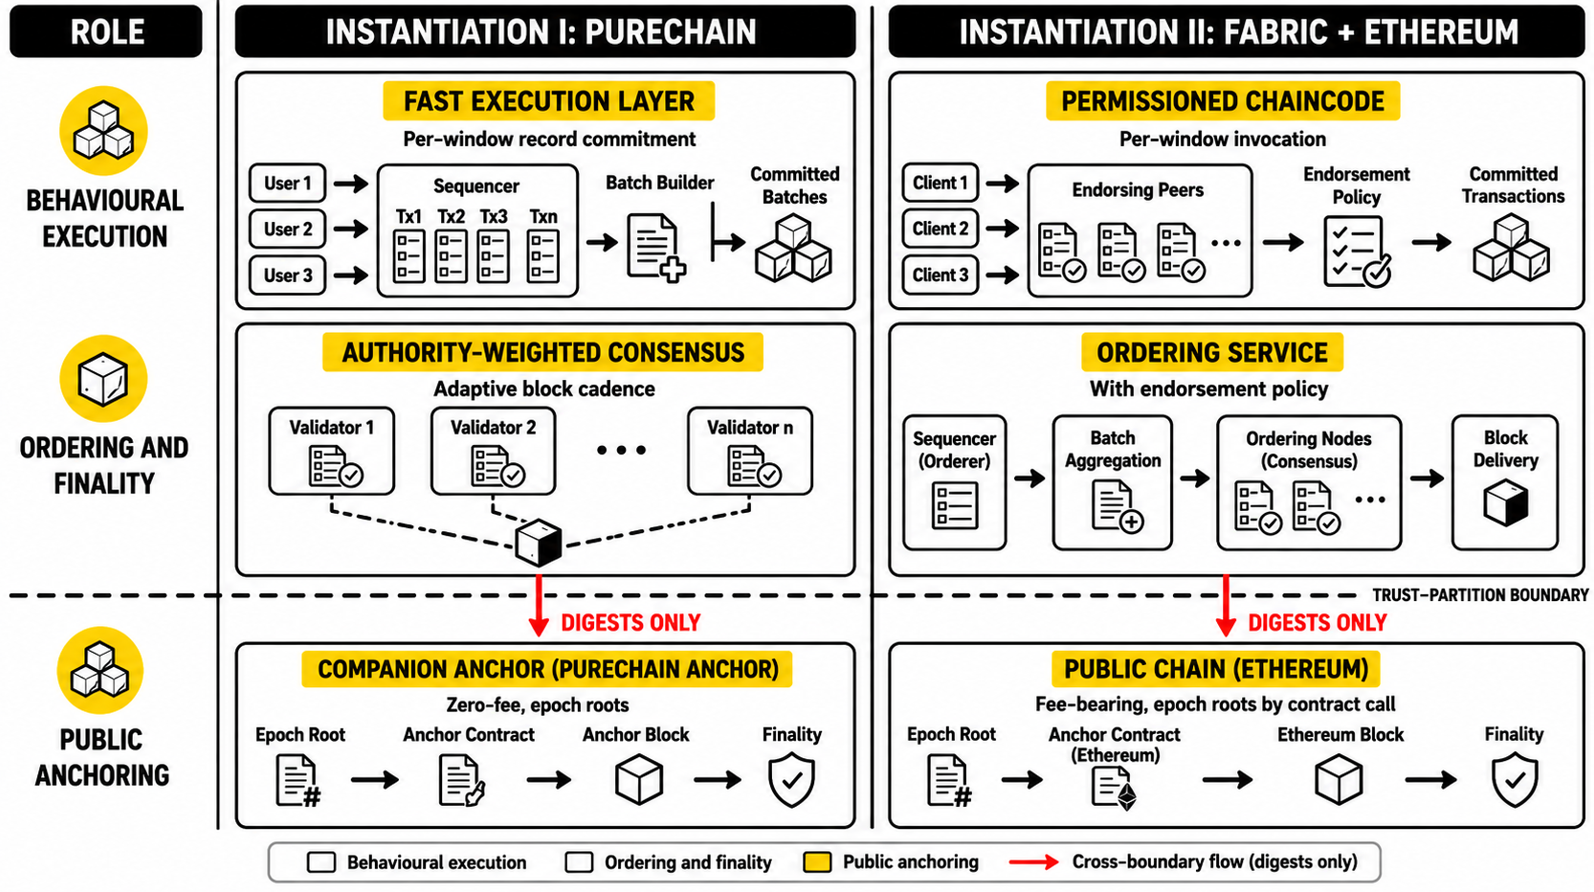
\includegraphics[width=1.00\textwidth]{figures/Picture21.PNG}
  \caption{The trust partition realised on PureChain NSL and on Fabric with Ethereum, with architectural roles held constant and the components discharging them substituted.}
  \label{fig:substrate-instantiation}
\end{figure}

\subsection{Experimental Environment}
\label{sec:substrate-environment}

Reproduction of either instantiation requires the substrate configuration, the class of device on which the constrained-side operations were executed, and the workload under which the measurements reported in the following chapter were taken. Tables~\ref{tab:env-instantiation-i} and~\ref{tab:env-instantiation-ii} record these in a common row order, so that a reader comparing them can see which quantities are substrate-dependent and which are not.

\begin{table}[tb]
  \centering
  \footnotesize
  \setlength{\tabcolsep}{5pt}
  \renewcommand{\arraystretch}{1.3}
  \caption{Experimental environment for Instantiation~I on PureChain NSL.}
  \label{tab:env-instantiation-i}
  \begin{tabularx}{\textwidth}{@{}
      >{\raggedright\arraybackslash}p{4.4cm}
      >{\raggedright\arraybackslash}X@{}}
    \toprule
    \textbf{Item} & \textbf{Configuration} \\
    \midrule
    Permissioned substrate & PureChain network \\
    Consensus mechanism & Authority-weighted consensus with adaptive block cadence \\
    Public anchor & PureChain public anchor, zero-fee; two public Ethereum networks used for comparison \\
    Smart-contract toolchain & Remix Ethereum IDE, Solidity compiler 0.8.10 \\
    Blockchain-side workload & One smart contract, four transaction types \\
    Network emulation & GNS3 \\
    Host operating system & Xubuntu, Xfce desktop \\
    Aggregator hardware & 251.4~GB RAM, 3.9~TB storage \\
    Constrained device profile & Client-side footprint of 0.17~MB model memory, 3.1~ms inference latency, 0.42~mJ per prediction, 167~kB update payload \\
    Learning framework & Flower 1.9.0, TensorFlow 2.9.0, Anaconda Navigator 2.6.1 \\
    Behavioural model & One-dimensional CNN-LSTM: 57 input units, 16 convolutional units with ReLU, softmax output over 8 classes \\
    Federation size & Five clients, aggregated on a single host \\
    Learning rates & 0.001 for client updates, 0.05 for global aggregation \\
    Datasets & CIC-Collections2023 public benchmark; and an internally generated lightweight IIoT dataset of 5{,}000 samples over 57 features, covering normal, denial-of-service, port-scan and brute-force traffic \\
    Training rounds & Twenty federated communication rounds \\
    \bottomrule
  \end{tabularx}
\end{table}

\begin{table}[tb]
  \centering
  \footnotesize
  \setlength{\tabcolsep}{5pt}
  \renewcommand{\arraystretch}{1.3}
  \caption{Experimental environment for Instantiation~II on Fabric with Ethereum.}
  \label{tab:env-instantiation-ii}
  \begin{tabularx}{\textwidth}{@{}
      >{\raggedright\arraybackslash}p{4.4cm}
      >{\raggedright\arraybackslash}X@{}}
    \toprule
    \textbf{Item} & \textbf{Configuration} \\
    \midrule
    Permissioned substrate & Hyperledger Fabric v2.5, Raft ordering \\
    Public substrate & Ethereum Geth v1.13, proof-of-work, 14~s mean block time, confirmation depth of three \\
    Topology & Five Fabric peers, one ordering service, one Geth node \\
    Block parameters & Two-second block interval, batch size of ten transactions \\
    Smart-contract toolchain & Remix IDE, Solidity compiler 0.8.17 \\
    Network emulation & Mininet v2.3.0, links at 10~Mbps and 1~Gbps \\
    Host operating system & Ubuntu 20.04.5 LTS \\
    Node hardware & Intel Xeon Gold 6230, 20 cores, 64~GB RAM, 2~TB SSD \\
    Constrained device class & Raspberry Pi 4, Cortex-A72, 4~GB RAM; ESP32 modules \\
    Edge workload & Lattice-encrypted payloads of 128 bytes at 10~Hz, signed and verified over five-minute steady-state runs \\
    Learning framework & TensorFlow 2.13, PennyLane 0.41.0, Anaconda Navigator 2.5.2 \\
    Behavioural model & CNN-LSTM trained centrally; no federation \\
    Dataset & NSL-KDD, 41 features, 5 classes, 80/20 stratified split \\
    Training configuration & Adam at learning rate 0.002, batch size 64, 15 epochs, ReLU activation, sparse categorical cross-entropy \\
    Transaction workload & 100 to 1000 simulated devices, 1000~tx/s on Fabric, cross-chain anchoring to Ethereum \\
    Repetition & Ten runs per measurement point, deviation below five per cent \\
    \bottomrule
  \end{tabularx}
\end{table}

The PureChain deployment is operated as a shared network rather than provisioned per experiment, so its validator membership and block cadence are fixed by the network operator and are not varied here. Identity and post-quantum operations were exercised on a separate bench rather than inside either ledger testbed, and Table~\ref{tab:env-identity} records that configuration. Keeping it distinct matters for interpretation: the encapsulation and compression measurements characterise the primitive on a workstation, not the cost of running it on the constrained devices listed above.

\begin{table}[tb]
  \centering
  \footnotesize
  \setlength{\tabcolsep}{5pt}
  \renewcommand{\arraystretch}{1.3}
  \caption{Environment for identity derivation and post-quantum key encapsulation.}
  \label{tab:env-identity}
  \begin{tabularx}{\textwidth}{@{}
      >{\raggedright\arraybackslash}p{4.4cm}
      >{\raggedright\arraybackslash}X@{}}
    \toprule
    \textbf{Item} & \textbf{Configuration} \\
    \midrule
    Host operating system & Windows 11 with WSL2, Ubuntu 24.04 LTS \\
    Hardware & Intel Core i7, 16~GB RAM \\
    Encapsulation mechanism & Kyber512, PQClean implementation \\
    Compression library & zlib v1.2.13 \\
    Implementation language & C, compiled with GCC \\
    Entropy seed length & 512 bits \\
    Ledger frameworks & Hyperledger Fabric for identity lifecycle; Ethereum on a Ganache testnet for revocation audit \\
    Scope of realisation & Identity derivation, compressed ciphertext delivery and reuse-aware decoding implemented; the ledger bridge specified but not implemented \\
    \bottomrule
  \end{tabularx}
\end{table}
The two environments differ in three respects that bear directly on how the following chapter should be read. Training is federated across five clients in the first instantiation and centralised in the second, so behavioural results are not directly comparable between them and are reported separately. The datasets likewise differ, the first instantiation evaluating on a public benchmark together with an internally generated IIoT set of 57 features and the second on NSL-KDD with 41 features across five classes. Anchoring economics differ by construction, the first instantiation writing to a zero-fee anchor and the second to a fee-bearing public chain with a fourteen-second block time and a confirmation depth of three.

What does carry across is the partition itself. Behavioural scoring is committed per observation window on a fast permissioned layer in both, finalisation is decided by a bounded identified validator set in both, and the material crossing to the public side is a digest in both. The measurements that follow are therefore reported per instantiation, and the cross-substrate claim rests on the structural correspondence. 
 

\chapter{Performance Evaluation and Result Discussion}
% \pagenumbering{arabic}
\Large
% \normalsize
\label{Chapter_5}

\section{Result Presentation and Analysis}
\label{sec:eval-presentation}

This section presents the simulation results and experimental findings that establish the performance capability, reliability, and efficiency of the proposed STRATA framework in delivering trustworthy security for constrained industrial deployments through behavioural trust scoring, permissioned finalisation, public anchoring, and quantum-resilient credential management. The analysis provides the justifiable basis for the claim that trust-partitioning delivers security within real device resource budgets, evaluated against the resource limits of industrial edge hardware and against comparable approaches drawn from the literature. Measurements are reported per instantiation and per architectural layer, so that each result can be traced to the stratum whose behaviour it characterises and to the research question it answers. Finally, the section presents the deployment scenarios under which the architecture was exercised, establishing that the reported behaviour holds under varying device populations, network conditions, and placement strategies rather than under a single favourable configuration.

\section{Performance Evaluation Metrics}
\label{sec:eval-metrics}

Assessment of the proposed framework spans four measurement domains, and a metric drawn from one domain cannot substitute for a metric drawn from another. Detection metrics establish whether behavioural evidence is trustworthy. Resource metrics establish whether the components producing that evidence fit the devices they are placed on. Ledger metrics establish whether commitment and anchoring are timely and affordable. Credential metrics establish whether identity derivation, key delivery, and withdrawal operate within the same budgets. The following subsections define each metric used, together with the interpretation that governs how its values are read in the results that follow.

\subsection{Accuracy ($A_{cc}$)}
\label{sec:metric-accuracy}

Accuracy quantifies the proportion of traffic samples assigned to their correct class across all classes, and is expressed by Equation~\eqref{eq:m-accuracy}.
\begin{equation}
\label{eq:m-accuracy}
A_{cc} \;=\; \frac{t_p + t_n}{t_p + t_n + f_p + f_n} ,
\end{equation}
where $t_p$ and $t_n$ are correct positive and negative predictions, and $f_p$ and $f_n$ are incorrect positive and negative predictions respectively. Accuracy is reported for completeness and comparability with prior work, but it is not the governing metric in this evaluation, since industrial traffic is dominated by normal behaviour and a detector predicting the majority class alone would score highly while supplying no usable evidence.

\subsection{Precision ($P_r$)}
\label{sec:metric-precision}

Precision quantifies the proportion of samples flagged as anomalous that are genuinely anomalous, and is defined by Equation~\eqref{eq:m-precision}.
\begin{equation}
\label{eq:m-precision}
P_r \;=\; \frac{t_p}{t_p + f_p} ,
\end{equation}
where $t_p$ and $f_p$ retain their earlier meanings. Precision carries particular weight in this architecture because behavioural evidence drives credential withdrawal. A low-precision detector supplies evidence that accumulates against healthy devices, and withdrawal being terminal, the cost of that error is a device removed from service and an enrolment repeated.

\subsection{Sensitivity ($R_c^{+}$)}
\label{sec:metric-sensitivity}

Sensitivity, equivalently positive recall, quantifies the proportion of genuinely anomalous samples the model identifies, and is given by Equation~\eqref{eq:m-sensitivity}.
\begin{equation}
\label{eq:m-sensitivity}
R_c^{+} \;=\; \frac{t_p}{t_p + f_n} ,
\end{equation}
where $f_n$ denotes anomalous samples the model failed to flag. A high sensitivity value indicates that compromised behaviour is detected rather than absorbed into the normal class, which determines whether the trust score declines at all when a device is misbehaving.

\subsection{Specificity ($R_c^{-}$)}
\label{sec:metric-specificity}

Specificity quantifies the proportion of normal traffic correctly recognised as normal, and is expressed by Equation~\eqref{eq:m-specificity}.
\begin{equation}
\label{eq:m-specificity}
R_c^{-} \;=\; \frac{t_n}{t_n + f_p} ,
\end{equation}
where $t_n$ and $f_p$ are correct and incorrect negative predictions. Specificity governs the stability of the credential population. A deployment with thousands of devices reporting continuously will accumulate false positives in proportion to its size, so specificity determines how much healthy traffic is misread as evidence against a device over an operating period.

\subsection{False Positive and False Negative Rates ($F_{pr}$, $F_{nr}$)}
\label{sec:metric-error-rates}

The error rates express the complements of the two preceding metrics directly, and are defined by Equation~\eqref{eq:m-error-rates}.
\begin{equation}
\label{eq:m-error-rates}
F_{pr} \;=\; \frac{f_p}{f_p + t_n} , \qquad
F_{nr} \;=\; \frac{f_n}{f_n + t_p} ,
\end{equation}
where $F_{pr}$ is the proportion of normal samples wrongly flagged and $F_{nr}$ the proportion of anomalous samples wrongly cleared. These two rates bound the two failure modes of the withdrawal mechanism: wrongful withdrawal of a healthy device is governed by $F_{pr}$, and retention of a compromised device is governed by $F_{nr}$.

\subsection{F1-score ($F_1$)}
\label{sec:metric-f1}

The F1-score is the harmonic mean of precision and sensitivity, given by Equation~\eqref{eq:m-f1}.
\begin{equation}
\label{eq:m-f1}
F_1 \;=\; 2 \times \frac{P_r \times R_c^{+}}{P_r + R_c^{+}} ,
\end{equation}
where $P_r$ and $R_c^{+}$ are as defined above. The harmonic form penalises imbalance between the two components, so a model achieving high sensitivity by flagging indiscriminately cannot compensate through volume. In an evaluation where both failure modes carry operational cost, F1 is the more trustworthy single indicator than accuracy.

\subsection{Cross-Entropy Loss ($\mathcal{L}$)}
\label{sec:metric-loss}

Convergence and prediction reliability during training are assessed through sparse categorical cross-entropy, expressed by Equation~\eqref{eq:m-loss}.
\begin{equation}
\label{eq:m-loss}
\mathcal{L} \;=\; -\frac{1}{N} \sum_{i=1}^{N} y_i \log \hat{y}_i ,
\end{equation}
where $N$ is the number of samples, $y_i$ the true label of sample $i$, and $\hat{y}_i$ the predicted probability assigned to that label. Falling loss across federated communication rounds indicates that aggregation is improving the global model rather than averaging away the contributions of individual clients, which is the failure mode federated training on non-identically distributed data is prone to.

\subsection{Model Memory Footprint ($M_f$)}
\label{sec:metric-memory}

Storage demanded by the behavioural model is determined by its parameter count and numeric representation, given by Equation~\eqref{eq:m-memory}.
\begin{equation}
\label{eq:m-memory}
M_f \;=\; \frac{P \times b}{10^{6}} ,
\end{equation}
where $P$ is the number of trainable parameters and $b$ the bytes per parameter, taken as four under single-precision encoding. Memory is the constraint that decides feasibility outright rather than gradually. A model exceeding the device budget cannot be deployed at any latency, so this metric determines whether behavioural scoring can occupy the stratum the architecture assigns it.

\subsection{Inference Latency ($T_{inf}$)}
\label{sec:metric-latency}

Time taken to score a single sample is averaged across the evaluation set, as given by Equation~\eqref{eq:m-latency}.
\begin{equation}
\label{eq:m-latency}
T_{inf} \;=\; \frac{1}{N} \sum_{i=1}^{N} \left( t_i^{out} - t_i^{in} \right) ,
\end{equation}
where $t_i^{in}$ and $t_i^{out}$ are the times at which sample $i$ enters and leaves the model. Inference latency determines whether scoring can run concurrently with the device's primary measurement and actuation duties without displacing them.

\subsection{Processor Utilisation ($U_{cpu}$)}
\label{sec:metric-cpu}

Processor utilisation is the proportion of available processor time occupied by continuous behavioural scoring, observed directly on the target platform at a stated sustained inference rate rather than derived from per-sample latency. It is reported alongside latency because a device may satisfy a latency requirement while leaving insufficient headroom for the function it was installed to perform.

\subsection{Energy per Inference ($E_{inf}$)}
\label{sec:metric-energy}

Energy consumed per prediction is estimated from computational volume, as given by Equation~\eqref{eq:m-energy}.
\begin{equation}
\label{eq:m-energy}
E_{inf} \;=\; \frac{\Phi}{10^{3}} \times \varepsilon ,
\end{equation}
where $\Phi$ is the number of floating-point operations per inference and $\varepsilon$ the energy attributed to each thousand such operations under the embedded-power estimation for low-power microcontrollers adopted in the published realisation of the behavioural module~\cite{amadi2026lightweight}. This metric determines operating life for battery-powered and energy-harvesting nodes, and is reported as an estimate obtained from that power model rather than as an instrumented measurement.

\subsection{Communication Overhead ($C_{ov}$)}
\label{sec:metric-comms}

Uplink demand imposed by each federated round is expressed by Equation~\eqref{eq:m-comms}.
\begin{equation}
\label{eq:m-comms}
C_{ov} \;=\; n \, s_{u} + s_{m} ,
\end{equation}
where $n$ is the number of participating clients, $s_{u}$ the size of a model update, and $s_{m}$ the size of the ledger metadata committed once for the round. Separating the two terms is deliberate, since it establishes what proportion of link consumption is attributable to the ledger rather than to learning, and therefore what the partition costs in bandwidth.

\subsection{Transaction Throughput ($N_{tps}$)}
\label{sec:metric-throughput}

Capacity of the permissioned layer is quantified by transactions completed per unit time, as given by Equation~\eqref{eq:m-throughput}.
\begin{equation}
\label{eq:m-throughput}
N_{tps} \;=\; \frac{N_{tx}}{T_{obs}} ,
\end{equation}
where $N_{tx}$ is the number of transactions committed and $T_{obs}$ the observation interval in seconds. Throughput is a function of block interval, block size, and consensus mechanism, and it determines whether the fast layer can absorb behavioural traffic as device population grows.

\subsection{Finalisation Latency ($T_{fin}$)}
\label{sec:metric-finality}

Delay between submission of a record and its irreversible commitment is expressed by Equation~\eqref{eq:m-finality}.
\begin{equation}
\label{eq:m-finality}
T_{fin} \;=\; t_{commit} - t_{submit} ,
\end{equation}
where $t_{submit}$ is the time of submission and $t_{commit}$ the time at which the record becomes final. Under deterministic consensus this quantity is complete on commitment, whereas under probabilistic consensus a confirmation depth must be added before the record may be relied upon, and the two are reported separately for that reason.

\subsection{Gas and Transaction Cost ($G_{c}$, $T_{c}$)}
\label{sec:metric-gas}

Computational resource consumed by a ledger operation is measured in gas, and the fee attaching to it is given by Equation~\eqref{eq:m-gas}.
\begin{equation}
\label{eq:m-gas}
T_{c} \;=\; G_{c} \times g_{p} ,
\end{equation}
where $G_{c}$ is the gas consumed by the operation and $g_{p}$ the prevailing gas price. Gas is a property of the operation and is comparable across networks; transaction cost depends additionally on the network and the moment, and is reported with its price assumptions stated.

\subsection{Compression Ratio and Payload Saving ($R_{c}$, $\Delta_{s}$)}
\label{sec:metric-compression}

Efficiency of the key delivery scheme is quantified by the ratio of delivered to original payload and the proportional saving, expressed by Equation~\eqref{eq:m-compression}.
\begin{equation}
\label{eq:m-compression}
R_{c} \;=\; \frac{S_{c}}{S_{o}} , \qquad
\Delta_{s} \;=\; \left( \frac{S_{o} - S_{c}}{S_{o}} \right) \times 100 ,
\end{equation}
where $S_{o}$ is the original ciphertext size and $S_{c}$ the size actually transmitted. On low-rate industrial links the delivered payload rather than the cryptographic computation dominates exchange cost, which is why this metric governs the feasibility of post-quantum migration on constrained hardware.

\subsection{Key Exchange Latency ($T_{kex}$)}
\label{sec:metric-kex}

Key exchange latency is the average end-to-end time required to establish shared session material between two parties, measured across repeated exchanges and reported together with the processor utilisation observed during them. Reporting the two together is necessary because a delivery scheme may reduce latency while raising processor load, and on a device with other duties that is not an improvement.

\subsection{Entropy Quality ($H_{\infty}$, $H$)}
\label{sec:metric-entropy}

Randomness of the seeds used in identifier derivation is assessed by min-entropy and Shannon entropy, given by Equation~\eqref{eq:m-entropy}.
\begin{equation}
\label{eq:m-entropy}
H_{\infty} \;=\; -\log_2 \max_i p_i , \qquad
H \;=\; -\sum_i p_i \log_2 p_i ,
\end{equation}
where $p_i$ is the observed probability of outcome $i$ across the sampled seeds. Min-entropy bounds the advantage available to an adversary guessing the most likely value and is therefore the conservative measure; Shannon entropy characterises the average uncertainty of the distribution.

\subsection{Trust Score Evolution and Revocation Condition}
\label{sec:metric-trust}

Device trust is maintained by the law of Plane~A (Section~\ref{sec:plane-a}). The isolation experiments of the second instantiation realise that law in its additive form, in which the score is credited for normal behaviour and penalised for anomalous behaviour at each cycle, as expressed by Equation~\eqref{eq:m-trust}.
\begin{equation}
\label{eq:m-trust}
s_i(t) \;=\; \min\!\Big(1,\; \max\!\big(0,\; s_i(t-1) + \Delta_{norm} - \Delta_{anom}\big)\Big) ,
\end{equation}
where $s_i(t)$ is the trust score of device $i$ at cycle $t$, $\Delta_{norm}$ the increment credited for normal behaviour, and $\Delta_{anom}$ the penalty applied when the behavioural score $q_i(t)$ falls below the flag threshold $\delta$. The additive form is the linear counterpart of the decay law of Equation~\eqref{eq:trust-decay}: it shares the same threshold semantics and the same terminal withdrawal, but a sustained anomaly lowers the score by a constant amount per cycle rather than geometrically, which makes the number of cycles to withdrawal exactly computable. Withdrawal is triggered by either of two independent conditions, expressed by Equation~\eqref{eq:m-revoke}.
\begin{equation}
\label{eq:m-revoke}
\mathrm{Revoke}(\mathrm{id}_i) \iff s_i(t) \leq \tau \;\; \text{or} \;\; S_i(t) > \mu_S ,
\end{equation}
where $\tau$ is the revocation threshold, $S_i(t)$ the anomaly streak counter, and $\mu_S$ the streak limit. The streak counter is maintained by Equation~\eqref{eq:m-streak}.
\begin{equation}
\label{eq:m-streak}
S_i(t) \;=\;
\begin{cases}
S_i(t-1) + 1, & \text{if an anomaly occurs at cycle } t, \\
0, & \text{if behaviour is normal at cycle } t.
\end{cases}
\end{equation}
The two conditions address different adversaries: the threshold catches gradual degradation accumulated over many cycles, and the streak catches abrupt compromise before the score has had time to fall.

\subsection{Revocation Latency ($T_{rev}$)}
\label{sec:metric-revocation-latency}

Elapsed time between the decision to withdraw and its confirmation on the ledger is expressed by Equation~\eqref{eq:m-revlat}.
\begin{equation}
\label{eq:m-revlat}
T_{rev} \;=\; t_{conf} - t_{flag} ,
\end{equation}
where $t_{flag}$ is the time at which the anomaly condition is satisfied and $t_{conf}$ the time at which the updated device status is confirmed. This quantity determines the window during which a device known to be misbehaving continues to hold a credential that relying parties still honour.

\subsection{Revocation Success Rate ($\eta_{rev}$)}
\label{sec:metric-revocation-rate}

Reliability of the withdrawal mechanism under load is quantified by Equation~\eqref{eq:m-revrate}.
\begin{equation}
\label{eq:m-revrate}
\eta_{rev} \;=\; \frac{N_{rev}}{N_{det}} \times 100 ,
\end{equation}
where $N_{det}$ is the number of anomalies detected and $N_{rev}$ the number resulting in a completed withdrawal within the allowed interval. A falling success rate under increasing device population would indicate that isolation degrades exactly when a deployment is largest, which is the condition under which the mechanism matters most.

\subsection{Score Normalisation for Heterogeneous Comparison}
\label{sec:metric-normalisation}

Comparison across metrics reported in different units and drawn from different sources requires mapping onto a common interval. For quantities in which larger values indicate better performance, normalisation follows Equation~\eqref{eq:m-norm-pos}.
\begin{equation}
\label{eq:m-norm-pos}
\mathcal{N}(x) \;=\; \frac{x - \min(x)}{\max(x) - \min(x)} ,
\end{equation}
where $x$ is the raw value of the quantity across the set of systems compared. For quantities in which smaller values are preferable, such as cost and latency, inverse normalisation follows Equation~\eqref{eq:m-norm-neg}.
\begin{equation}
\label{eq:m-norm-neg}
\mathcal{N}(L) \;=\; 1 - \frac{L - \min(L)}{\max(L) - \min(L)} ,
\end{equation}
where $L$ is the raw value of the cost or latency quantity. Normalised scores are bounded, relative, and interpretable without arbitrary weighting, and they support statements about relative position only. Ratios between normalised scores carry no meaning, and results reported on this basis are read accordingly.


\section{Result Discussion}
\label{sec:eval-discussion}

The result discussion focuses on the reliability and generalisation of the behavioural trust module across heterogeneous industrial traffic, the learning stability and error minimisation of the trimmed convolutional recurrent detector, the resource economy that permits it to occupy the edge stratum, the timeliness and cost of permissioned finalisation, the verified soundness of the contracts carrying the write path, the affordability of quantum-resilient identity and key delivery on constrained hardware, the responsiveness of decay-driven credential withdrawal, and the realisation of the same partition on two unrelated ledger substrates, using the performance evaluation metrics defined earlier.

\subsection{Reliable Behavioural Evidence Across Heterogeneous Traffic}
\label{sec:eval-evidence}
 
Behavioural scoring supplies the evidence on which every subsequent decision in the architecture depends, so its reliability is established across three datasets rather than on a single benchmark. The values in Table~\ref{tab:res-detection} summarise detection performance on the public benchmark, the internally generated industrial set, and NSL-KDD as used on the second instantiation.
 
\begin{table}[!htbp]
  \centering
  \footnotesize
  \setlength{\tabcolsep}{5pt}
  \renewcommand{\arraystretch}{1.3}
  \caption{Detection performance of the behavioural trust module across the three datasets used.}
  \label{tab:res-detection}
  \begin{tabularx}{\textwidth}{@{}
      >{\raggedright\arraybackslash}p{3.6cm}
      >{\raggedright\arraybackslash}X
      >{\raggedright\arraybackslash}X
      >{\raggedright\arraybackslash}X
      >{\raggedright\arraybackslash}X
      >{\raggedright\arraybackslash}X
      >{\raggedright\arraybackslash}X@{}}
    \toprule
    \textbf{Dataset} & \textbf{$A_{cc}$ (\%)} & \textbf{$P_r$ (\%)} & \textbf{$R_c^{+}$ (\%)} & \textbf{$F_1$ (\%)} & \textbf{$F_{pr}$ (\%)} & \textbf{$F_{nr}$ (\%)} \\
    \midrule
    CIC-Collections2023 & 97.70 & n/r & 97.70 & 97.70 & n/r & n/r \\
    Internal IIoT set & 96.84 & n/r & 96.33 & 96.52 & n/r & n/r \\
    NSL-KDD & 97.40 & 95.10 & 98.20 & 96.80 & 1.90 & 0.70 \\
    \bottomrule
  \end{tabularx}
  \vspace{2pt}
  \parbox{\linewidth}{\footnotesize n/r: not reported for that dataset. NSL-KDD values are those of the published realisation~\cite{amadi2026symmetric}, in which precision, recall, and F1 are reported as model-level scores, while the false positive and false negative rates are derived from the normalised five-class confusion matrix. Because the two sets are computed on different bases, F1 is not the harmonic mean of the tabulated precision and recall, and the false negative rate is not the complement of the tabulated recall.}
\end{table}
 
First, the module demonstrated consistently high detection capability, with accuracy spanning 96.84\% to 97.70\% across datasets built by different means and carrying different attack classes. The strongest aggregate result was obtained on the public benchmark at 97.70\% accuracy with F1 at the same value, and the weakest on the internally generated industrial set at 96.84\% accuracy and 96.52\% F1. That the weakest case is the synthetic industrial set rather than a curated public benchmark is the informative outcome, since the industrial set carries device-level noise, protocol variation, and lightweight attack signatures that curated benchmarks omit. A spread of 0.86 percentage points between the easiest and hardest of the three indicates that the detector is not leaning on the particular traffic patterns of any one of them.
 
Secondly, for sensitivity, the findings in Table~\ref{tab:res-detection} indicate that positive recall ranges between 96.33\% and 98.20\%, implying that compromised behaviour is detected rather than absorbed into the normal class. The highest sensitivity, 98.20\% on NSL-KDD, is accompanied by the lowest precision in the table at 95.10\%. That pairing is the expected trade and is the direction an isolation mechanism should favour, since a device wrongly flagged accumulates evidence gradually and may recover, whereas a device wrongly cleared continues to operate under a credential the architecture still honours.

 \begin{figure}[!htbp]
  \centering
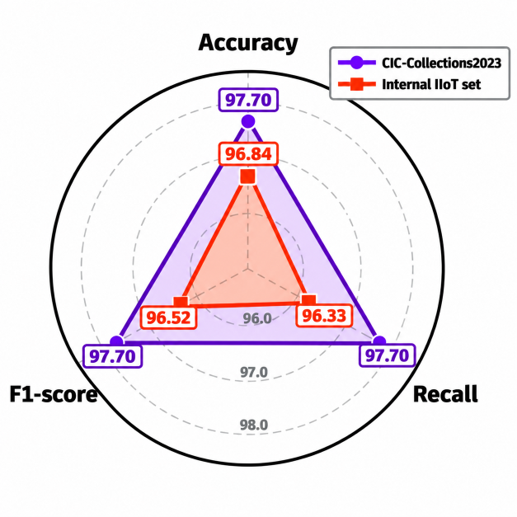
\includegraphics[width=0.72\textwidth]{figures/Picture22.png}
  \caption{Accuracy, recall and F1-score of the behavioural module, closely aligned across the public benchmark and the internal industrial set.}
  \label{fig:res-envelope}
\end{figure}

Thirdly, the error rates bound the two failure modes of the withdrawal mechanism directly. A false positive rate of 1.90\% and a false negative rate of 0.70\% were recorded on the dataset for which both are reported. The false positive figure governs the stability of the credential population, determining how much healthy traffic is misread as evidence against a device over an operating period, and the false negative figure governs exposure, determining the proportion of anomalous behaviour that never reaches the trust score at all. Most misclassifications corresponded to transient network bursts labelled as denial-of-service traffic, which is the benign direction for this failure to take, since a burst misread as an attack degrades a trust score recoverably while an attack misread as a burst does not.
 
Fourthly, generalisation between the public benchmark and the industrial set is visible as a shape rather than a scalar. Figure~\ref{fig:res-envelope} plots accuracy, recall, and F1 for both datasets on common axes, and the two performance envelopes remain closely aligned across all three measures. Alignment of that kind matters more in a federated setting than a single aggregate figure, because non-identically distributed clients are the condition under which a detector most readily specialises to one distribution, and a model that had done so would show divergent envelopes rather than parallel ones.
Lastly, per-class behaviour determines whether the aggregate figures can be relied upon at all, since a detector carrying its average on the dominant class supplies evidence that is systematically weakest exactly where an adversary operates. Figure~\ref{fig:res-perclass} reports per-class F1 on the public benchmark and the normalised confusion structure on NSL-KDD, the two being different quantities and not directly comparable to one another.
 \begin{figure}[!htbp]
  \centering
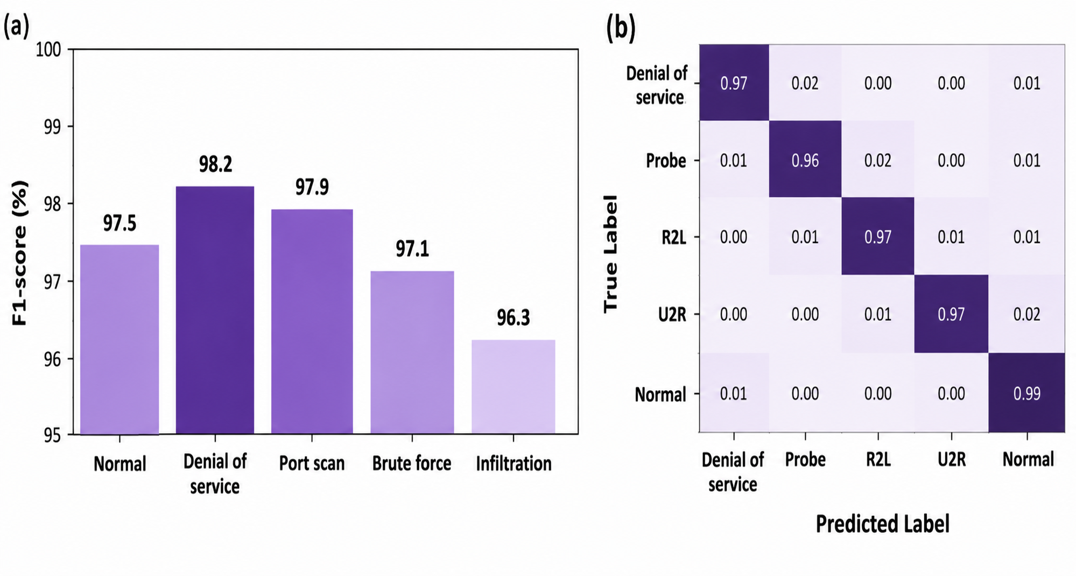
\includegraphics[width=0.98\textwidth]{figures/Picture23.png}
  \caption{Per-class F1-score on CIC-Collections2023 (a) and the normalised confusion matrix on NSL-KDD (b).}
  \label{fig:res-perclass}
\end{figure}
 

Detection capability is uniform across attack categories rather than concentrated in the dominant class. On the public benchmark the strongest class is denial of service at 98.20\% and the weakest is infiltration at 96.30\%, a spread of 1.90 percentage points. On NSL-KDD the diagonal runs from 0.99 for normal traffic to 0.96 for probe activity, a spread of 3.00 percentage points, with no class below 0.96. Infiltration and probe activity occupying the lower positions is consistent with their character, since both are low-volume categories whose traffic most closely resembles ordinary operation and both are consequently the categories a volumetric detector would miss. The off-diagonal structure confirms that the residual confusion is small and evenly distributed rather than systematic, since no off-diagonal cell exceeds 0.02 and no class loses more than four per cent of its samples in total. Withdrawal decisions therefore rest on evidence whose reliability does not depend on which attack a device is subject to.
Taken together, the aggregate figures, the error rates, the aligned envelopes, and the per-class uniformity establish that the behavioural stratum produces evidence of sufficient quality and consistency to drive a terminal decision.


\subsection{Learning Stability and the Cost of Federating}
\label{sec:eval-learning}

The behavioural module is claimed to operate inside constrained device budgets without sacrificing detection performance. The preceding subsection established what that performance is; this one establishes what it cost to obtain it under the arrangement the architecture imposes. Two costs are at issue. Distributing optimisation across clients that observe different traffic may yield a weaker global model than training on pooled data would, and a model may reach an acceptable final score by a path unstable enough that the score would not survive a different division of the data. Neither cost is visible in a final accuracy figure, so both are examined directly. The values in Table~\ref{tab:res-rounds} set the federated configuration against a centralised control trained on the same data at sampled communication rounds.

\begin{table}[!htbp]
  \centering
  \footnotesize
  \setlength{\tabcolsep}{5pt}
  \renewcommand{\arraystretch}{1.3}
  \caption{Federated and centralised configurations compared at sampled communication rounds.}
  \label{tab:res-rounds}
  \begin{tabularx}{\textwidth}{@{}
      >{\raggedright\arraybackslash}p{2.2cm}
      >{\raggedright\arraybackslash}X
      >{\raggedright\arraybackslash}X
      >{\raggedright\arraybackslash}X
      >{\raggedright\arraybackslash}X@{}}
    \toprule
    \textbf{Round} & \textbf{Centralised $F_1$} & \textbf{Centralised $\mathcal{L}$} & \textbf{Federated $F_1$} & \textbf{Federated $\mathcal{L}$} \\
    \midrule
    1  & 0.026 & 1.945 & 0.026 & 1.950 \\
    5  & 0.791 & 1.060 & 0.790 & 1.070 \\
    10 & 0.965 & 0.119 & 0.964 & 0.121 \\
    15 & 0.961 & 0.133 & 0.961 & 0.114 \\
    20 & 0.981 & 0.086 & 0.978 & 0.088 \\
    \bottomrule
  \end{tabularx}
\end{table}

The penalty for distributing optimisation is 0.003 in F1 at the twentieth round, 0.978 against 0.981, and it never exceeds that figure at any sampled point. Cost differs by no more than 0.019 across the same rounds. A margin of three thousandths is smaller than the fold-to-fold variation reported later in this subsection, which places it below the resolution at which the two configurations can be meaningfully separated. The architecture places scoring at the edge to keep traffic on the device that generated it and to stay inside the memory budget of that device; had federating cost several points of F1, those reasons would have to be weighed against a materially weaker detector. They do not.

Optimisation is front-loaded. Between the first and fifth rounds F1 rises by 0.764 and cost falls by 0.880, accounting for the greater part of the total movement in both, and the curves flatten by approximately the eighth round, after which the remaining schedule contributes little. A deployment constrained in communication rather than computation can therefore obtain most of the available performance from a short training schedule, which matters because each round costs 167~kB per client on the uplink.

One round runs against the trend and is worth examining rather than averaging away. At the fifteenth round the centralised control loses ground, its F1 falling from 0.965 to 0.961 and its cost rising from 0.119 to 0.133, while the federated configuration eases only from 0.964 to 0.961 in F1 and continues to reduce cost from 0.121 to 0.114. At the single point where the two diverge, the distributed arrangement is the steadier of the two. Averaging updates drawn from clients observing different traffic evidently damps the variance a single optimiser exhibits rather than amplifying it, which is the opposite of the behaviour usually anticipated when data is not identically distributed. Figure~\ref{fig:res-convergence} shows all four detection measures across the full schedule.

\begin{figure}[!htbp]
  \centering
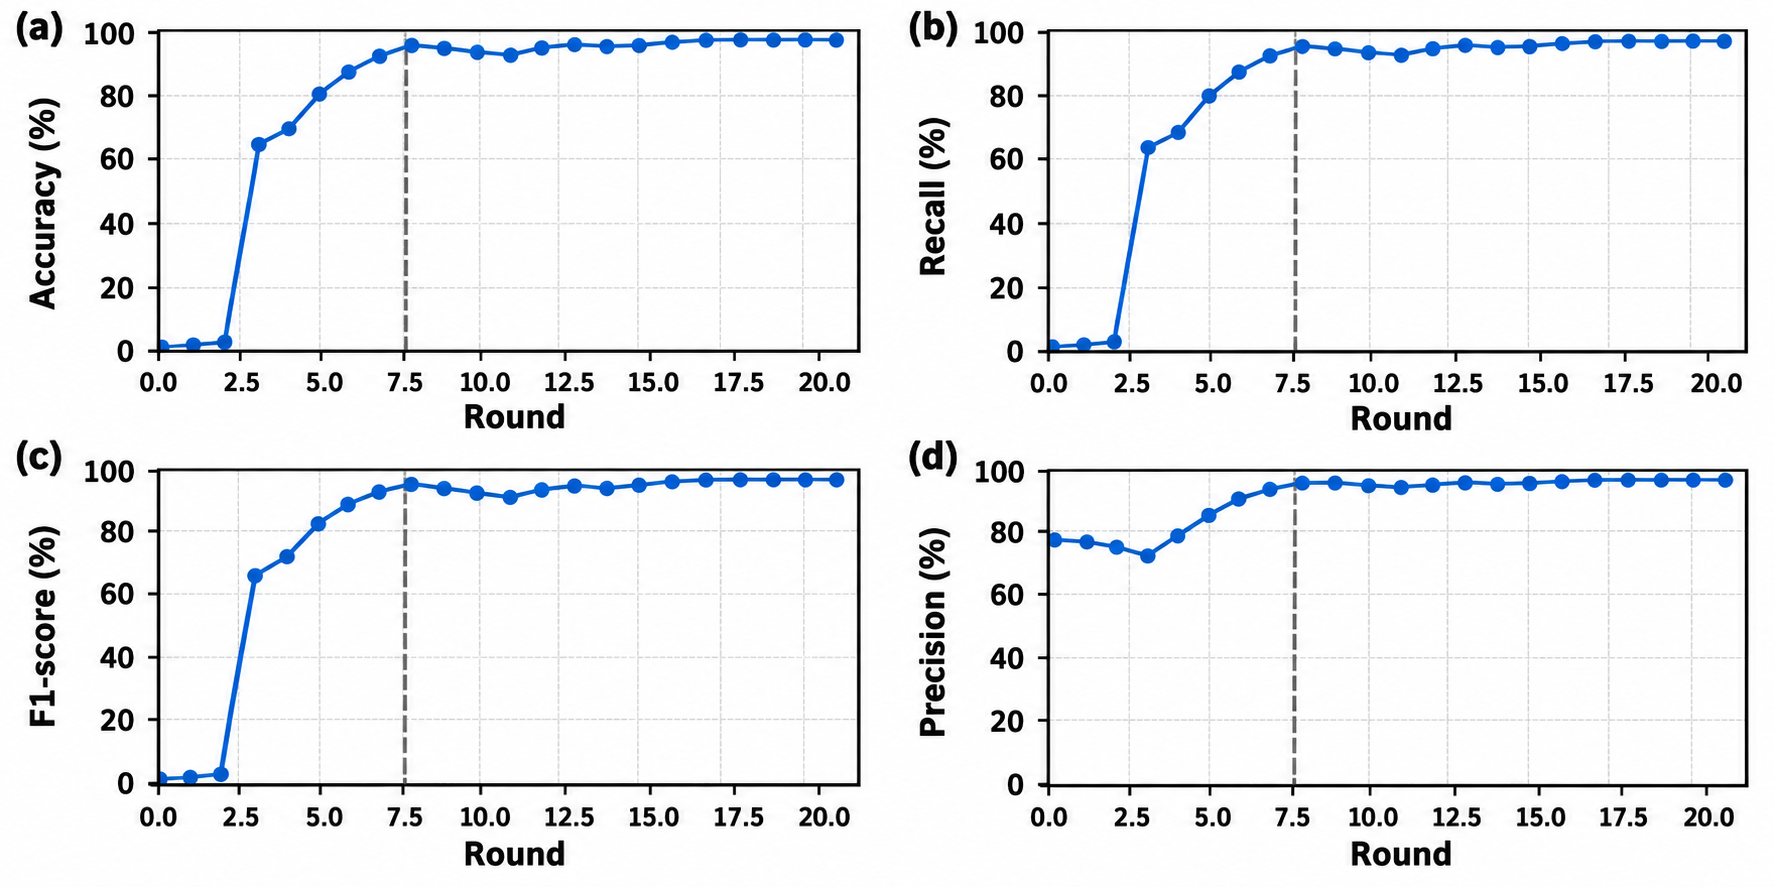
\includegraphics[width=\textwidth]{figures/Fig5_convergence_author.png}
  \caption{Convergence of accuracy (a), recall (b), F1-score (c) and precision (d) across twenty federated communication rounds on CIC-Collections2023.}
  \label{fig:res-convergence}
\end{figure}

Precision behaves unlike the other three measures from the very first round, and the difference carries operational weight. Accuracy, recall and F1 all begin near zero and climb steeply from the third round, whereas precision opens at approximately 76\% and never falls below 72\%. The model is therefore reluctant to flag healthy traffic from the outset, before it has learned to recognise anomalous traffic at all, and it acquires that recognition without becoming indiscriminate. For a mechanism that withdraws credentials terminally, this ordering is the favourable one. A model exhibiting the reverse profile, flagging readily at the start and learning restraint later, would pass through an interval during which it withdrew credentials from devices that had done nothing wrong, and no subsequent improvement would repair that. Recall and F1 track accuracy throughout the schedule, so the reduction in missed anomalies is not obtained by degrading the balance between the two error types.

Convergence on the internally generated industrial set is examined separately. That set is smaller, synthetic, and built to a different generation process, so agreement in final scores does not by itself establish that the model reached them by a comparable route. Figure~\ref{fig:res-internal} shows the progression there, plotted against training epochs rather than the communication rounds used above, since convergence on that set was tracked at the level of the local optimiser. The three measures rise together from approximately 85\% and settle at 96.84\%, 96.33\% and 96.52\% by roughly the thirtieth epoch, without oscillation, crossing, or late drift. The ordering holds throughout, with accuracy above F1 and F1 above recall at every point, so the three measures improve in concert rather than trading against one another.


\begin{figure}[!htbp]
  \centering
  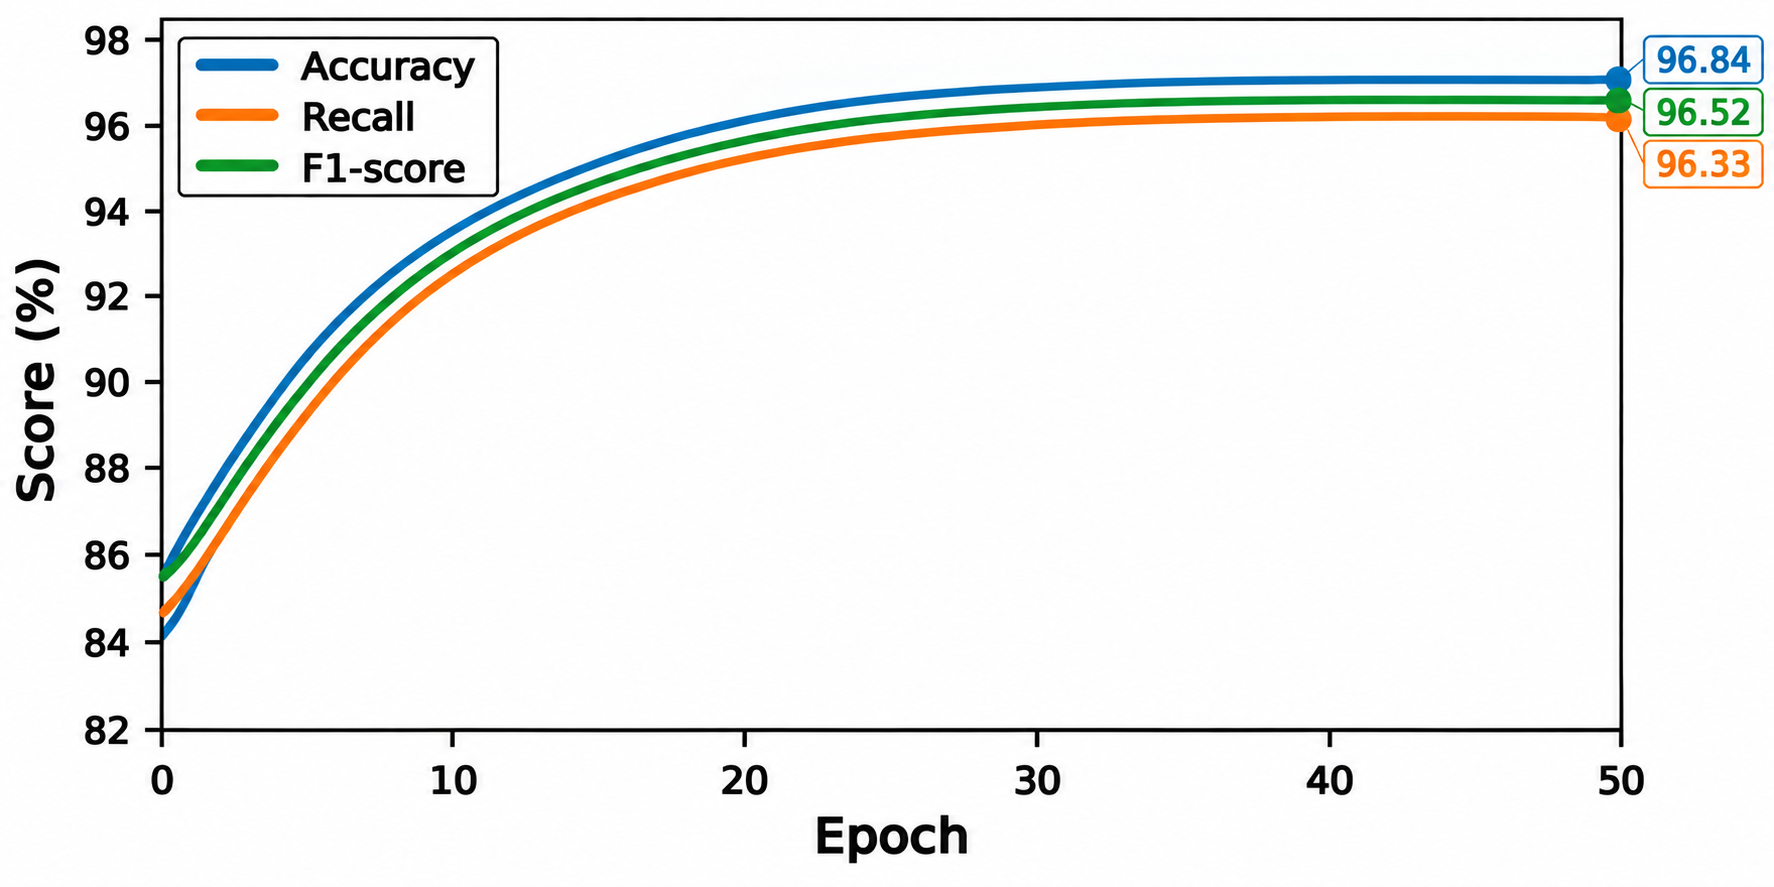
\includegraphics[width=0.80\textwidth]{figures/Fig5_internal_convergence_author.png}
  \caption{Convergence of accuracy, recall and F1-score of the behavioural module across training epochs on the internal IIoT dataset.}
  \label{fig:res-internal}
\end{figure}

The second cost concerns reproducibility rather than magnitude. A model may converge smoothly on one division of the data and differently on another, and a trust score computed from such a model would inherit that dependence. Five-fold cross-validation on both datasets tests it, and the values in Table~\ref{tab:res-cv} summarise the result.

\begin{table}[!htbp]
  \centering
  \footnotesize
  \setlength{\tabcolsep}{5pt}
  \renewcommand{\arraystretch}{1.3}
  \caption{Five-fold cross-validation on the public benchmark and the internal industrial set.}
  \label{tab:res-cv}
  \begin{tabularx}{\textwidth}{@{}
      >{\raggedright\arraybackslash}p{5.0cm}
      >{\raggedright\arraybackslash}X
      >{\raggedright\arraybackslash}X@{}}
    \toprule
    \textbf{Measure} & \textbf{CIC-Collections2023} & \textbf{Internal IIoT set} \\
    \midrule
    Mean accuracy & 97.65\% & 96.52\% \\
    Standard deviation & 0.31\% & 0.38\% \\
    Mean F1-score & 97.58\% & 96.41\% \\
    \bottomrule
  \end{tabularx}
\end{table}

Variation across folds stays below 0.40\% on both datasets, at 0.31\% on the public benchmark and 0.38\% on the industrial set, and the cross-validated means fall within 0.32 percentage points of the single-split results, at 97.65\% against 97.70\% and 96.52\% against 96.84\%. Dividing the data five ways therefore moves the outcome by less than the gap between the two datasets themselves, and the intervals drawn in Figure~\ref{fig:res-cv} are correspondingly narrow. The relevance to the architecture is specific rather than general: a trust score is accumulated from repeated evaluations, so a detector whose output shifted with the partition would produce withdrawals that reflected the training split as much as the behaviour of the device, and no threshold could be set against such a score with confidence.

\begin{figure}[!htbp]
  \centering
  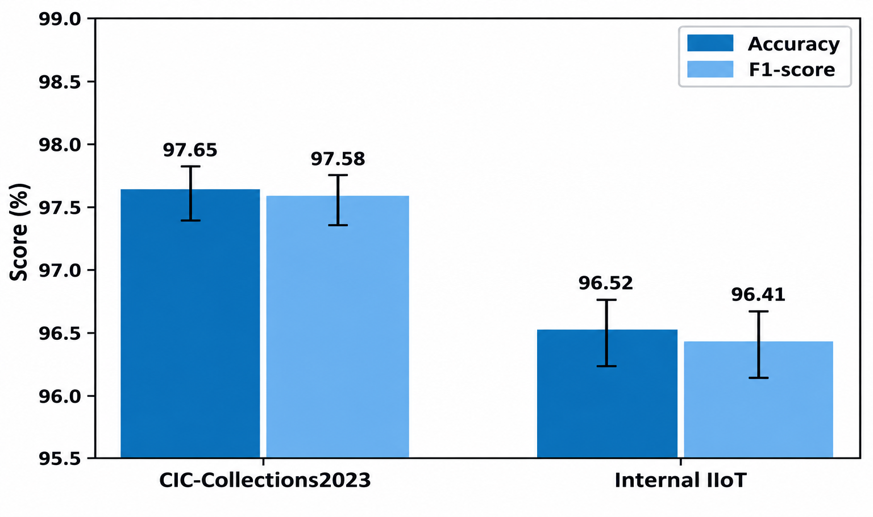
\includegraphics[width=\textwidth]{figures/Picture26.png}
  \caption{Five-fold cross-validated accuracy and F1-score on CIC-Collections2023 and the internal IIoT dataset. Error bars show one standard deviation of accuracy across folds.}
  \label{fig:res-cv}
\end{figure}

Stability on the second instantiation was established by a different method, which matters because agreement between two methods is stronger evidence than repetition of one. There the detector was trained centrally on an eighty-twenty stratified split and evaluated across five independent runs under identical conditions, with deviation across runs held under five per cent and the reported accuracy and F1 taken as means rather than best cases. Partitioning tests whether a result survives a different division of the data; repetition tests whether it survives a different initialisation of the same division. The first instantiation passes the former and the second passes the latter, and neither exposes a dependence that would undermine a score accumulated over time.

The two costs the architecture might have incurred by distributing behavioural scoring are therefore both small and both measured. Federating costs at most 0.003 in F1 against pooled training, and the result varies by under 0.40\% across partitions of either dataset. Detection performance is consequently not sacrificed by the placement decision, which settles the second half of the question this module was built to answer; whether the model that delivers it fits the compute, memory, and energy budgets of the device it runs on is settled separately by the resource analysis that follows.

\subsection{Lightweight Resource Utilisation and Deployment Feasibility}
\label{sec:eval-resource}

The two preceding subsections establish that behavioural scoring produces dependable evidence and that distributing it costs almost nothing in quality. Neither addresses the harder half of the question, which is whether the model producing that evidence can run on the device the architecture assigns it to. The distinction matters because the two failure modes are not alike. A detector that scores poorly is a weak component in a sound architecture; a detector that does not fit is a refutation of the placement decision itself, since behavioural evaluation would have to be relocated to a gateway or a server and the case for keeping traffic on the device that generated it would collapse with it. Feasibility is therefore assessed against the four budgets an industrial node actually holds, namely storage, time, processor occupancy, and energy, together with the uplink the federated arrangement consumes.

Table~\ref{tab:res-budget} sets each measured quantity against the constraint it must satisfy.

\begin{table}[!htbp]
  \centering
  \footnotesize
  \setlength{\tabcolsep}{5pt}
  \renewcommand{\arraystretch}{1.3}
  \caption{Measured resource demand of the behavioural module against the budget each quantity is constrained by.}
  \label{tab:res-budget}
  \begin{tabularx}{\textwidth}{@{}
      >{\raggedright\arraybackslash}p{4.4cm}
      >{\raggedright\arraybackslash}p{3.0cm}
      >{\raggedright\arraybackslash}X@{}}
    \toprule
    \textbf{Quantity} & \textbf{Measured} & \textbf{Constraint it sits against} \\
    \midrule
    Trainable parameters & 41{,}762 & Flash and working memory of microcontroller-class nodes \\
    Model storage under single-precision encoding & 0.17~MB & Typical 1 to 2~MB device memory budget \\
    Peak memory including activation buffers & Below 0.6~MB & The same budget, under inference load rather than at rest \\
    Inference latency & 3.1~ms per sample & Timing of the control loop the device participates in \\
    Processor occupancy at 50 inferences per second & 6 to 9\% & Headroom required by the measurement and actuation duties of the node \\
    Energy per prediction & 0.42~mJ & Power budget of a battery or harvested supply \\
    Federated update payload per round & 167~kB per client & Uplink capacity of low-rate industrial links \\
    Ledger metadata per round & 180 to 220~bytes & The same uplink, shared with the learning traffic \\
    \bottomrule
  \end{tabularx}
\end{table}

Peak memory is the decisive figure among these, and it is decisive in a way the others are not. Storage of 0.17~MB at rest rises to below 0.6~MB once activation buffers are allocated during inference, against a device budget of one to two megabytes, so the model occupies at most three fifths of the smaller budget and leaves the remainder to the application the node was installed to run. Latency and occupancy admit degradation, since a slower device can score less frequently and still function, but memory does not: a model exceeding the available allocation cannot be loaded at any inference rate, which makes this the quantity on which the placement decision stands or falls.

Processor occupancy between 6\% and 9\% at fifty inferences per second is the second constraint worth emphasising, because it is the one an industrial engineer will ask about first. A node whose primary duty is measurement and actuation cannot surrender its processor to a security function, and an occupancy figure in single digits leaves the schedule essentially intact. Energy at 0.42~mJ per prediction bears on a different deployment class, namely nodes drawing on battery or harvested supply, for which the relevant question is operating life rather than schedulability.

The ledger contributes almost nothing to the uplink it shares with the learning traffic, and Figure~\ref{fig:res-uplink} shows the proportion directly. Each round carries a model update of approximately 167~kB per client, to which the ledger adds between 180 and 220 bytes of commitment metadata. At a single client that metadata is 0.132\% of the round; at ten clients it is 0.013\%, and the per-round uplink requirement remains below 1.7~MB, within the capacity of low-power wide-area, wireless local, and industrial Ethernet links alike. The share falls as clients are added because the commitment is made once per round rather than once per client, so the ledger overhead is amortised across the federation rather than multiplied by it, and a larger deployment pays proportionally less for participation than a smaller one.

This proportion is the correct one for the architecture. The ledger exists to commit evidence about behaviour, and an arrangement in which commitment consumed a material share of the link carrying that behaviour would have inverted the relationship between the two. The on-chain validation accompanying each commitment consumes 65{,}618 gas and completes in approximately 0.11~s, so the computational cost of committing evidence is borne by the permissioned layer rather than by the device.
\begin{figure}[!htbp]
  \centering
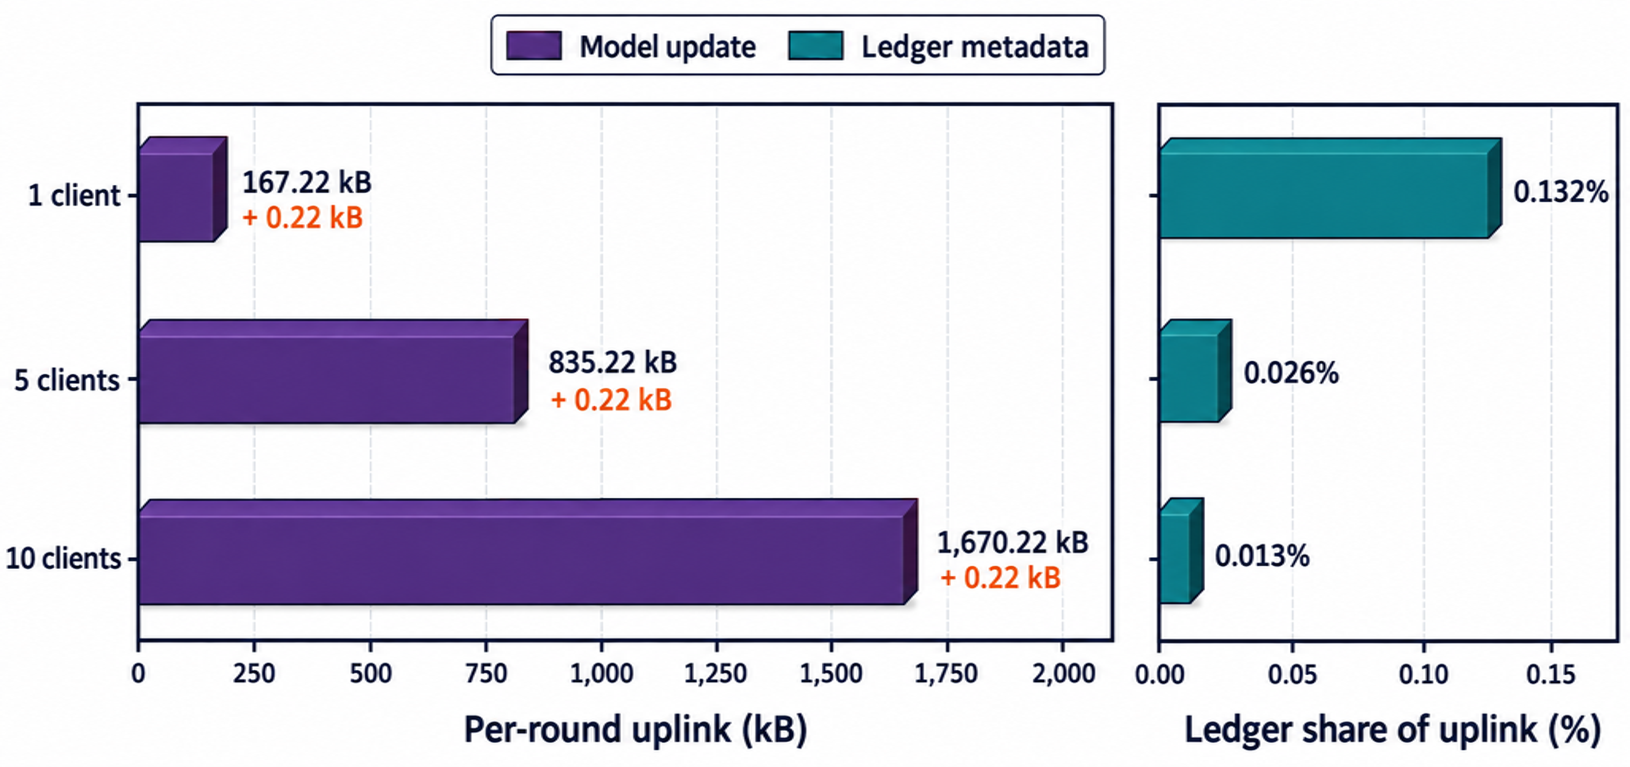
\includegraphics[width=\textwidth]{figures/Picture28.png}
  \caption{Per-round uplink composition at one, five and ten participating clients, split between the federated model update and the ledger commitment metadata, with the ledger share shown separately.}
  \label{fig:res-uplink}
\end{figure}
Whether these figures are favourable in absolute terms is established by comparison. Table~\ref{tab:res-overhead} sets the behavioural module against architectures reported in comparable federated ledger-backed detection work.
\begin{table}[!htbp]
  \centering
  \footnotesize
  \setlength{\tabcolsep}{4pt}
  \renewcommand{\arraystretch}{1.3}
  \caption{Resource profile of the behavioural module against architectures reported in comparable federated ledger-backed detection work.}
  \label{tab:res-overhead}
  \begin{tabularx}{\textwidth}{@{}
      >{\raggedright\arraybackslash}p{3.1cm}
      >{\raggedright\arraybackslash}p{1.7cm}
      >{\raggedright\arraybackslash}p{1.4cm}
      >{\raggedright\arraybackslash}p{1.4cm}
      >{\raggedright\arraybackslash}p{1.4cm}
      >{\raggedright\arraybackslash}p{1.3cm}
      >{\raggedright\arraybackslash}X@{}}
    \toprule
    \textbf{Architecture} & \textbf{Parameters} & \textbf{$M_f$ (MB)} & \textbf{$T_{inf}$ (ms)} & \textbf{$E_{inf}$ (mJ)} & \textbf{$C_{ov}$ (kB)} & \textbf{Suitability} \\
    \midrule
    Generative adversarial detector~\cite{enhanced} & 8.7\,M & 10.5 & 22.7 & 4.5 & 812 & High overhead \\
    EfficientNet-B0~\cite{FLBC-IDS} & 4.0\,M & 5.3 & 18.4 & 3.1 & 560 & High overhead \\
    Capsule autoencoder~\cite{Anitha2} & 1.2\,M & 1.8 & 11.2 & 1.9 & 240 & Medium \\
    Convolutional and multilayer hybrid~\cite{Metaverse} & 620\,k & 0.9 & 9.5 & 1.2 & 180 & Medium \\
    Behavioural module & 41{,}762 & 0.17 & 3.1 & 0.42 & 167 & Lightweight \\
    \bottomrule
  \end{tabularx}
\end{table}

The behavioural module is the least demanding architecture in the comparison on every column. Against the capsule autoencoder it carries roughly one twenty-ninth of the parameters, and against the generative adversarial detector roughly one two-hundredth. Inference is between three and seven times faster than the four comparators, at 3.1~ms against a range of 9.5 to 22.7~ms. Energy per prediction is between three and eleven times lower, at 0.42~mJ against 1.2 to 4.5~mJ. The update payload is the one column where the margin is slight, at 167~kB against 180~kB for the nearest comparator, which is expected since payload size follows parameter count only loosely once encoding overheads are included.

The column that decides feasibility, however, is memory, and there the comparison is not a matter of degree. Only the behavioural module and the convolutional hybrid fall inside a one to two megabyte allocation at rest, and once activation buffers are accounted for the margin narrows further. The capsule autoencoder at 1.8~MB consumes the entire budget before inference begins; the two largest comparators exceed it several times over. An architecture built on any of the three cannot place scoring on a microcontroller-class node at all, and must therefore site behavioural evaluation at a gateway or in the cloud. Figure~\ref{fig:res-feasibility} plots the comparison against the budget directly.


\begin{figure}[!htbp]
  \centering
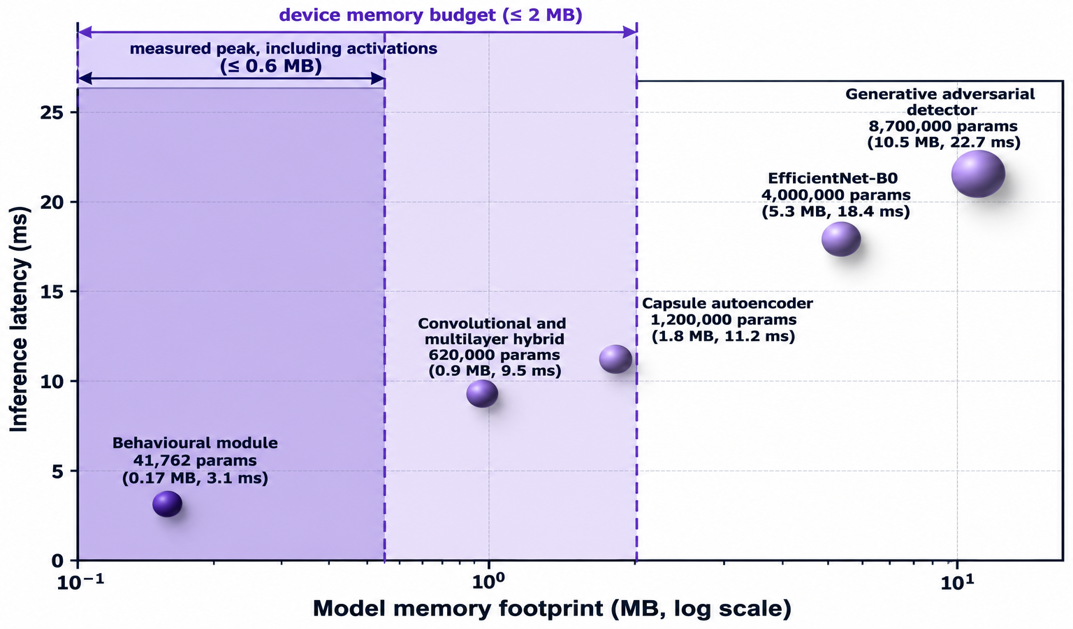
\includegraphics[width=\textwidth]{figures/Picture27.png}
  \caption{Memory footprint against inference latency for the behavioural module and four comparator architectures, with marker area proportional to parameter count and the device memory budget shaded.}
  \label{fig:res-feasibility}
\end{figure}

Two qualifications belong with these figures and are better stated here than discovered later. The energy value is an estimate obtained from an embedded-power model of a low-power microcontroller~\cite{amadi2026lightweight}, rather than a measurement taken from an instrumented device, and it should be read as an order-of-magnitude indication for the comparison rather than as a device-specific value. The latency and occupancy figures were obtained on an ARM Cortex-A53 class environment, which sits at the capable end of the constrained spectrum; a microcontroller-class part with a lower clock would be slower in proportion, though the memory figures that decide feasibility would be unchanged, since they follow from parameter count and encoding rather than from processor speed.

The resource evidence therefore settles the half of the question the two preceding subsections left open. Behavioural scoring fits within the compute, memory, and energy budgets of constrained industrial hardware, with the binding constraint satisfied at under three fifths of the smaller budget, and the ledger participation the architecture requires adds under two tenths of one per cent to the link the device already uses. Taken with the detection results, the module operates inside real device budgets without sacrificing detection performance, which is what the behavioural stratum was required to demonstrate.

\subsection{Efficient Permissioned Finalisation and Ledger Economy}
\label{sec:eval-ledger}

Behavioural evidence acquires standing only once it has been ordered and committed, and the layer performing that commitment sits directly in the path between detection and response. Two properties therefore decide whether the partition is workable in an industrial setting. Commitment must complete inside the interval within which the plant can still act on what was detected, since evidence finalised after the moment for response has passed is a record rather than a control input. And the cost of committing must remain proportionate to the frequency at which behavioural evidence arrives, because the fast layer receives a verdict for every observation window and every device, and a per-commitment cost that is merely acceptable in isolation becomes prohibitive when multiplied by that traffic. The measurements in this subsection address both, together with the consensus characteristics from which they follow.

Table~\ref{tab:led-functions} reports the cost of each contract operation carrying the write path.

\begin{table}[!htbp]
  \centering
  \footnotesize
  \setlength{\tabcolsep}{5pt}
  \renewcommand{\arraystretch}{1.3}
  \caption{Contract operations carrying the write and read paths on the permissioned instantiation, with the cost of each.}
  \label{tab:led-functions}
  \begin{tabularx}{\textwidth}{@{}
      >{\raggedright\arraybackslash}p{3.2cm}
      >{\raggedright\arraybackslash}p{2.4cm}
      >{\raggedright\arraybackslash}p{2.0cm}
      >{\raggedright\arraybackslash}X@{}}
    \toprule
    \textbf{Operation} & \textbf{Transaction cost} & \textbf{Gas} & \textbf{Role in the architecture} \\
    \midrule
    Model commitment & 64{,}778 & 65{,}618 & Commits a validated behavioural update to the permissioned layer; recurs once per observation window \\
    Server registration & 45{,}258 & 45{,}638 & Admits an aggregation server to the consortium; once per server \\
    Model retrieval & Nil & Nil & Read path used by verification and audit; unbounded in frequency \\
    \bottomrule
  \end{tabularx}
\end{table}

Commitment of a validated update consumes 65{,}618 gas and completes in approximately 0.11~s. That interval is the figure on which the partition depends, and its significance lies in what it excludes as much as in its magnitude. Because authority is assigned rather than contested, a block is final at the moment it is committed, so the 0.11~s constitutes the entire delay rather than the first instalment of one. A probabilistic mechanism reaching the same nominal interval would additionally require a confirmation depth before the record could be relied upon, and the accumulated wait would place commitment outside the window within which a supervisory loop can still act. A device flagged by the behavioural stratum can therefore be acted upon within the same cycle in which it was flagged.

The two write operations differ in how their frequency scales, and the final column of the table records that difference because it governs which cost matters. Model commitment recurs once per observation window for every participating client, so it dominates the operating cost of the layer. Server registration at 45{,}638 gas occurs once per aggregation server and is a deployment cost rather than an operating one. Retrieval costs nothing at all, and that asymmetry is deliberate rather than incidental. Verification is the operation an auditor performs, potentially frequently and potentially without any relationship to the consortium whose conduct is under examination. A design charging for reads would impose a toll on precisely the party whose scrutiny the anchoring stratum exists to invite, and would make the cost of auditing rise with the thoroughness of the audit. Writes are paid for by the operator who benefits from them; reads are free to whoever wishes to check.

Whether these costs are favourable relative to alternatives is established by comparison against public networks executing equivalent operations. Figure~\ref{fig:led-gas} reports gas consumed across the permissioned network and two public networks for three admission and commitment operations. The set compared is not identical to the set tabulated above: model commitment appears in both, while central-server registration and device registration are exercised only in the cross-network comparison and retrieval, costing nothing, is omitted from it. The central-server registration in the figure, at about 51{,}000 gas, is the value reported in the cross-network comparison of the published realisation~\cite{amadi2026lightweight} and differs from the 45{,}638 gas recorded for server registration in Table~\ref{tab:led-functions}, which comes from the deployment cost measurement of the same work. The figure is therefore read for the direction of the difference between networks rather than against the table.


\begin{figure}[!htbp]
  \centering
  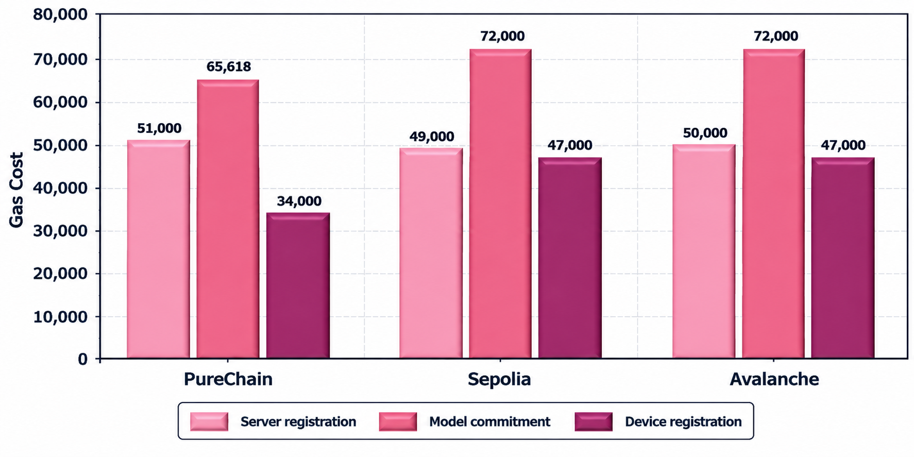
\includegraphics[width=\textwidth]{figures/Picture30.png}
  \caption{Gas consumed by the contract operations on the permissioned network and on two public networks.}
  \label{fig:led-gas}
\end{figure}

The permissioned network consumes less gas than either public network on two of the three operations compared. Model commitment costs 65{,}618 against approximately 72{,}000 on both public networks, and device registration approximately 34{,}000 against approximately 47{,}000, while central-server registration is slightly higher at roughly 51{,}000 against 49{,}000 and 50{,}000. The margin is therefore widest on device registration, and that ordering matters more than the aggregate saving. Device registration is performed once per device, so a plant that doubles its instrumented population doubles its expenditure on that operation, whereas server registration occurs once for the consortium regardless of size. The operation on which the partition saves most is the one whose total grows with the installation, and the operation on which it saves least is the one performed only at commissioning. The comparison establishes direction rather than deployment cost, since gas measures computational work and the fee attaching to it depends on the network and the moment, but the direction is the property the partition requires: high-frequency operations must be affordable on the layer to which they are assigned.
The characteristics producing these costs are those of the consensus mechanism itself. Figure~\ref{fig:led-consensus} compares it against three families in common use across the five dimensions bearing on constrained deployment.


\begin{figure}[!htbp]
  \centering
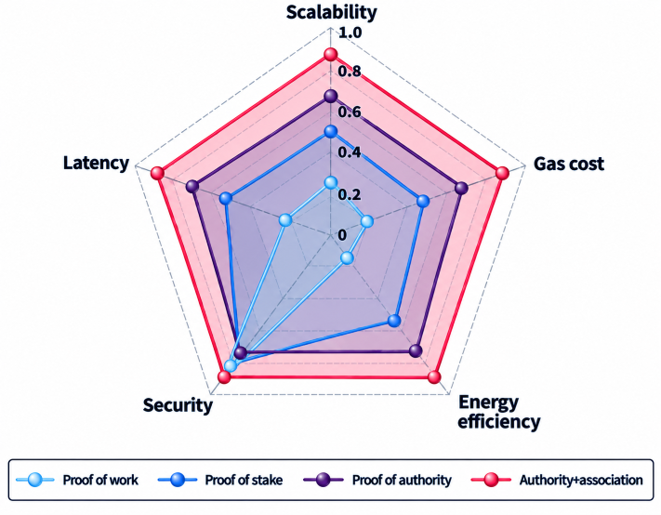
\includegraphics[width=\textwidth]{figures/Picture29.png}
  \caption{Normalised comparison of consensus mechanisms across five dimensions bearing on constrained deployment. Values are relative indicators on a unit interval rather than absolute measurements.}
  \label{fig:led-consensus}
\end{figure}

A qualification governs how this comparison may be read and is stated before the interpretation rather than after it. Only the proposed mechanism derives from direct measurement in this work. The three baselines are drawn from published experimental and simulation studies conducted under their own conditions, and all values are mapped onto a unit interval so that quantities reported in different units can be placed alongside one another. The figure therefore supports statements about relative position and supports no statement about ratios between mechanisms.

Read within that limit, the shapes rather than the individual values carry the argument. Proof of work forms a narrow spike, reaching 0.90 on security and falling to 0.15 on energy efficiency and 0.20 on gas cost, which is the profile of a mechanism that purchases assurance with expended work. The two intermediate mechanisms form progressively rounder polygons as that expenditure is reduced. The proposed mechanism encloses all three on every axis except one, and the exception is the informative part of the figure: on security it meets proof of work at 0.90 rather than exceeding it. A mechanism claiming both the lowest cost and the highest assurance would invite the suspicion that the acceptance rule had been relaxed to obtain the saving, and the figure does not make that claim.

The remainder of the profile follows from the partition rather than from the consensus mechanism alone. Scalability and latency improve together, at 0.90 on both against 0.70 and 0.75 for the nearest comparator, because high-frequency validation is separated from long-term immutable storage, so throughput does not degrade as participating devices multiply. The two properties that ordinarily trade against one another are decoupled by the partition rather than balanced within a single layer. Gas and energy efficiency improve, at 0.90 and 0.92, because authority is assigned rather than contested, which removes both proof generation and global leader election from the commitment path. The efficiency is therefore obtained by constraining who may participate, not by weakening what participation requires of them, which is why the security axis holds rather than falling.

The behaviour of the layer when its validator set is degraded completes the picture. Beyond the tolerated number of simultaneously unavailable validators, block finalisation may be delayed and new update metadata cannot be committed while the condition persists. The consequence is narrower than it appears, and it is narrower for an architectural reason rather than an incidental one. Nodes continue inference and local monitoring against the most recently verified global model, so detection is uninterrupted while commitment is stalled, and what degrades is the frequency with which the model is refreshed rather than the presence of monitoring. Integrity is preserved throughout, since unvalidated updates are rejected by access-control enforcement and by hash and dimension consistency checks and cannot reach the immutable layer. When availability is restored, aggregation and anchoring resume without rollback or loss of model consistency.

That behaviour follows directly from placing behavioural scoring below the consensus layer rather than above it. An architecture requiring consensus before a device could be evaluated would lose detection entirely under the same conditions, since no verdict could be produced until agreement was restored. Partitioning the two converts a consensus outage from a loss of coverage into a loss of freshness, and freshness is much the cheaper of the two to surrender in a plant that must continue operating while its ledger recovers.

The permissioned layer therefore satisfies both properties the partition requires of it. Commitment is final in approximately 0.11~s with no confirmation depth to wait out, which places it inside the interval within which a supervisory loop can still act; and the cost per commitment is lower than equivalent operations on public networks, with the widest margin falling on the operation whose frequency grows with the deployment. What the layer cannot supply, and was never intended to supply, is protection against the consortium that operates it, which is the responsibility of the anchoring stratum examined next.

\subsection{Verifiable Contract Security and Threat Resistance}
\label{sec:eval-security}
Performance establishes that the permissioned layer commits evidence quickly and cheaply. It establishes nothing about whether that evidence can be trusted once an adversary is assumed, and the distinction is sharper here than in most systems because the contracts carrying the write path are themselves the enforcement mechanism. A detector may be accurate, a consensus mechanism fast, and a commitment final, while a defect in the contract admits an unauthorised write that renders all three irrelevant. Assurance at this layer is therefore assessed in two ways that answer different questions: formal auditing of the contract source, which asks whether the implementation contains known classes of defect, and threat-model analysis, which asks whether the mechanisms deployed answer the capabilities an adversary is assumed to hold.

The contracts underwent static and dynamic vulnerability assessment under two complementary tools, a cloud-based formal verification platform and a static analysis framework for contract source, across six vulnerability classes. Table~\ref{tab:sec-audit} summarises the outcome.

\begin{table}[!htbp]
  \centering
  \footnotesize
  \setlength{\tabcolsep}{5pt}
  \renewcommand{\arraystretch}{1.3}
  \caption{Contract vulnerability assessment across the six classes examined.}
  \label{tab:sec-audit}
  \begin{tabularx}{\textwidth}{@{}
      >{\raggedright\arraybackslash}p{4.4cm}
      >{\raggedright\arraybackslash}p{2.4cm}
      >{\raggedright\arraybackslash}X@{}}
    \toprule
    \textbf{Vulnerability class} & \textbf{Status} & \textbf{Basis} \\
    \midrule
    Reentrancy & None found & Control-flow analysis \\
    Access control & Passed & Role checks validated \\
    Integer overflow and underflow & None found & Arithmetic safety enforced \\
    Gas inefficiencies & Minor & Optimised before deployment \\
    Timestamp manipulation & None found & Validators cross-check commit time \\
    External call risks & None found & No untrusted external calls \\
    \midrule
    Overall assessment & 98\% & Combined tool score \\
    \bottomrule
  \end{tabularx}
\end{table}

The overall figure expresses the proportion of examined classes returning no critical or high-severity finding, and its composition matters more than its magnitude. A single class was flagged, gas inefficiency, at minor severity, and it was optimised before deployment. That is the least consequential of the six for this architecture, since gas efficiency governs operating cost rather than integrity, and a contract that is expensive but sound commits the same evidence as a cheap one. The classes whose failure would have compromised the anchoring guarantee all returned clean. Reentrancy would have permitted a partially completed commitment to be re-entered and the ledger state corrupted mid-write. Arithmetic overflow would have permitted a crafted value to wrap a counter or an index and write outside its intended bounds. An unsafe external call would have handed control to code outside the audited surface during a commitment. None was found, and the absence of all three is what allows the commitment path to be treated as trustworthy in the sense the architecture requires.

Timestamp manipulation deserves separate comment, since timestamps appear in every commitment the architecture publishes and an unverifiable commit time would weaken precisely the audit trail the anchoring stratum exists to provide. The mitigation available here is one that an open network cannot offer. Validators cross-check the commit time against their own clocks, and a validator proposing an implausible timestamp is identified and attributable rather than anonymous, so the misbehaviour carries a consequence beyond rejection of the block. The residual exposure is bounded by the disagreement tolerated among validator clocks, which is a configuration parameter set by the consortium rather than an open-ended risk.

Auditing establishes that the implementation is free of known defect classes. It does not establish that the mechanisms present are sufficient against an adversary who is assumed capable rather than opportunistic, which requires the threat model. The model assumes honest but curious aggregation servers, authenticated channels, and semi-trusted validators, so an adversary is presumed able to observe legitimately and to attempt influence from within rather than merely to intrude from outside. Figure~\ref{fig:sec-threat} sets out the assets exposed under those assumptions, the capabilities attributed to an adversary, and the mechanisms deployed in response.


\begin{figure}[!htbp]
  \centering
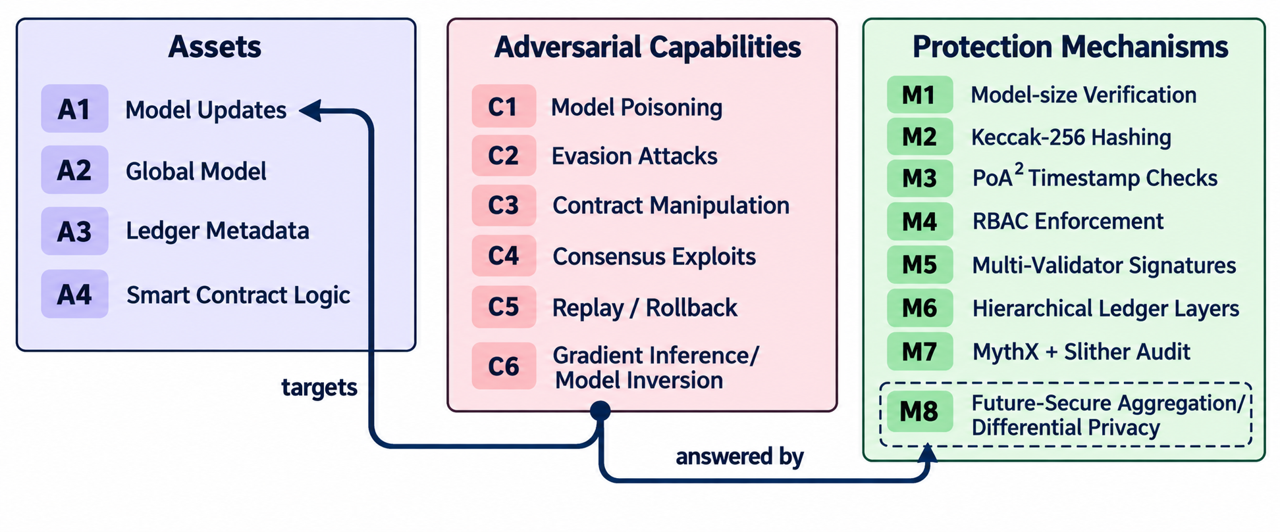
\includegraphics[width=\textwidth]{figures/Picture31.png}
  \caption{System assets, assumed adversarial capabilities, and the protection mechanisms deployed against them.}
  \label{fig:sec-threat}
\end{figure}

Most capabilities in the model are answered by a mechanism already in place. Model poisoning is met by model-size verification and dimension consistency checks, which reject an update whose shape departs from the agreed architecture before it can influence aggregation. Contract manipulation is met by role-based access control, which confines each operation to the participants entitled to invoke it. Consensus exploitation is met by multi-validator signature verification, which requires a quorum rather than a single authority. Replay and rollback are met by timestamp-based protection, which is the mechanism the audit examined separately and found sound. Ledger metadata is protected by hashing, and the layered ledger design confines the consequences of a compromise at one layer to that layer.

One capability is not answered by a deployed mechanism, and the architecture states so rather than leaving it to inference. Gradient inference and model inversion target the model updates in transit, and the present design exchanges those updates without additional cryptographic aggregation or noise injection. That choice was made deliberately, since secure aggregation and differential privacy both impose computation or accuracy costs on nodes whose budgets the preceding subsection showed to be tight, and the architecture prioritised deployability. Within the evaluated threat model the exposure is mitigated rather than eliminated: an adversary must first become an authenticated participant, updates are validated on receipt, and provenance is recorded on the ledger, so inference would have to be attempted from a position that is itself attributable. Under stronger adversarial assumptions the theoretical risk remains, and secure aggregation is designated as the mechanism answering it and identified as a priority extension rather than claimed as present.

That is the honest boundary of what this layer demonstrates. The contracts are free of the defect classes that would undermine commitment, the mechanisms deployed answer five of the six capabilities the model attributes to an adversary, and the sixth is named, its exposure bounded by the participation requirements of the consortium, and its remedy specified for future work. What no amount of contract assurance can supply is protection against the consortium itself, since every mechanism examined here is operated by the parties whose conduct an auditor may wish to examine, and it is that residual exposure the anchoring stratum exists to close.

\subsection{Optimised Quantum-Resilient Identity and Key Delivery}
\label{sec:eval-identity}
Every commitment examined so far carries a device identifier, and every exchange that produces one rests on a cryptographic assumption. Migration to post-quantum primitives is usually argued as a question of whether the replacements are secure, which they are by construction and by standardisation. On constrained hardware the question that decides deployment is different, since lattice ciphertexts and public keys are substantially larger than the elliptic-curve material they replace, and on a low-rate industrial link the bytes cost more than the arithmetic. This subsection therefore assesses fit rather than strength: whether an identifier can be derived on a field device without administrative discretion, and whether the key material protecting it can be delivered within the same budgets the behavioural module was shown to respect.

An identifier assigned administratively can be reassigned administratively, which places the operator inside the trust boundary of every claim subsequently made about the device. Deriving the identifier from entropy captured at the device removes that discretion, and Table~\ref{tab:id-comparison} sets the construction against the two alternatives available to a constrained deployment.

\begin{table}[!htbp]
  \centering
  \footnotesize
  \setlength{\tabcolsep}{5pt}
  \renewcommand{\arraystretch}{1.3}
  \caption{Identity construction compared against static and hardware-fingerprint alternatives.}
  \label{tab:id-comparison}
  \begin{tabularx}{\textwidth}{@{}
      >{\raggedright\arraybackslash}p{4.4cm}
      >{\raggedright\arraybackslash}p{2.6cm}
      >{\raggedright\arraybackslash}p{2.2cm}
      >{\raggedright\arraybackslash}X@{}}
    \toprule
    \textbf{Construction} & \textbf{Spoof resistance} & \textbf{Entropy bits} & \textbf{Adaptability} \\
    \midrule
    Address and timestamp & Low & Approximately 32 & None \\
    Hardware fingerprint with metadata & Medium & Approximately 64 & Static \\
    Entropy-seeded derivation & High & 128 and above & Real time \\
    \bottomrule
  \end{tabularx}
\end{table}

Two columns carry the argument, and they carry different halves of it. The entropy column governs whether the identifier can be published. An identifier of approximately 32 bits is enumerable, so an adversary observing the anchor could reconstruct the device population by exhaustion; at 128 bits and above it cannot, which is what permits the hashed identifier to appear on the public substrate without turning the audit record into an inventory of the plant. The adaptability column governs whether the identifier can participate in withdrawal at all. A static construction fixes what a device is and says nothing about how it behaves, so a deployment using one must maintain revocation state entirely outside the identity layer, in a register that is itself administered by the operator. A construction admitting real-time trust evolution keeps the credential and the behavioural record bound together, which is the property the withdrawal mechanism of the architecture depends upon.

Entropy quality was assessed across a thousand derived seeds of 128 bits each, with min-entropy concentrating around 0.95 and Shannon entropy falling between 0.99 and 1.0, indicating near-uniform bit distributions. The qualification stated when the plane was specified applies directly to those figures and is repeated here rather than left to the reader's memory: the sampler is software, so the measurements characterise the uniformity and reproducibility of a simulated source rather than the unpredictability a hardware generator would supply. What they do establish is that the derivation consumes and conditions its input correctly, which is the part of the construction a hardware substitution would leave unchanged, since the sample enters the digest as an opaque bit string.

Delivery of key material is where post-quantum migration is paid for on a constrained link, and Table~\ref{tab:pq-compression} reports what the delivery scheme recovers. All reductions are stated against the 768-byte Kyber512 ciphertext, which is the quantity actually transmitted.

\begin{table}[!htbp]
  \centering
  \footnotesize
  \setlength{\tabcolsep}{5pt}
  \renewcommand{\arraystretch}{1.3}
  \caption{Ciphertext size under generic and reuse-aware compression, against the 768-byte Kyber512 ciphertext.}
  \label{tab:pq-compression}
  \begin{tabularx}{\textwidth}{@{}
      >{\raggedright\arraybackslash}p{5.0cm}
      >{\raggedright\arraybackslash}X
      >{\raggedright\arraybackslash}X
      >{\raggedright\arraybackslash}X@{}}
    \toprule
    \textbf{Scheme} & \textbf{Raw size (bytes)} & \textbf{Delivered size (bytes)} & \textbf{Reduction} \\
    \midrule
    Baseline encapsulation & 768 & 768 & 0\% \\
    Generic compression & 768 & 510 & 33.6\% \\
    Reuse-aware delivery & 768 & 410 & 46.6\% \\
    \bottomrule
  \end{tabularx}
\end{table}

Generic compression recovers a third of the payload at 33.6\% and the reuse-aware scheme recovers close to half at 46.6\%, and the difference between the two is where the contribution lies rather than in the magnitude of either. Generic compression treats each ciphertext as an isolated object and must therefore compress the whole of it on every exchange. The reuse-aware scheme exploits a property of the traffic instead: successive ciphertexts to the same peer share most of their content, so the payload is fragmented, unchanged fragments are not retransmitted, and only the delta is compressed. The delivered sizes are those of the published realisation of this module~\cite{amadi2025quantum}; the reductions differ from the 36.3\% and 48.75\% reported there only because that work expressed them against the 800-byte Kyber512 public key, whereas the quantity actually transmitted, and the reference used here, is the 768-byte ciphertext.

Figure~\ref{fig:pq-delivery} shows where the difference between the two schemes comes from. Panel (a) gives the size achieved by compressing the Kyber512 ciphertext across four transmission cases, at 520, 540, 510 and 495 bytes, so generic compression alone delivers between 64\% and 71\% of the original in every case, close to the 510-byte figure of Table~\ref{tab:pq-compression}. Panel (b) gives the property the reuse-aware scheme exploits. Of the sixty-four fragments into which the ciphertext is partitioned, 51 were unchanged between transmissions and 13 changed, so most of the payload was already held by the receiver. Suppressing the retransmission of those fragments, and compressing only what changed, is what takes the delivered size from the 495 to 540 bytes of compression alone down to 410 bytes. The effectiveness of the scheme is therefore bounded by how stable the ciphertext is between sessions rather than by how compressible it is in isolation, and it retains its efficiency under mutation as the number of modified bytes rises from sixty to a hundred and twenty.


\begin{figure}[!htbp]
  \centering
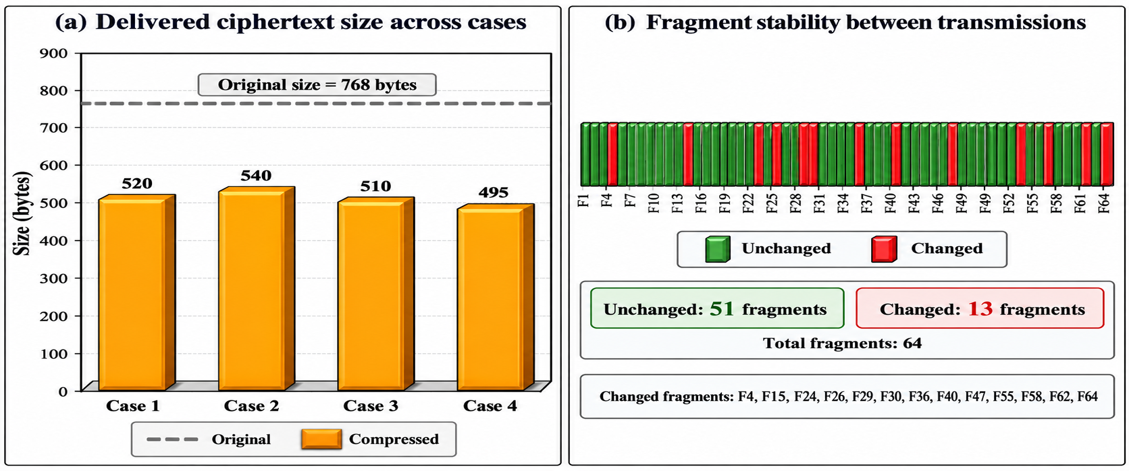
\includegraphics[width=\textwidth]{figures/Picture34.png}
  \caption{Delivered ciphertext size across simulation cases (a) and fragment stability between successive transmissions (b).}
  \label{fig:pq-delivery}
\end{figure}

The effect on the exchange itself is reported in Figure~\ref{fig:pq-latency}, and the middle bar of each panel is the instructive one.


\begin{figure}[!htbp]
  \centering
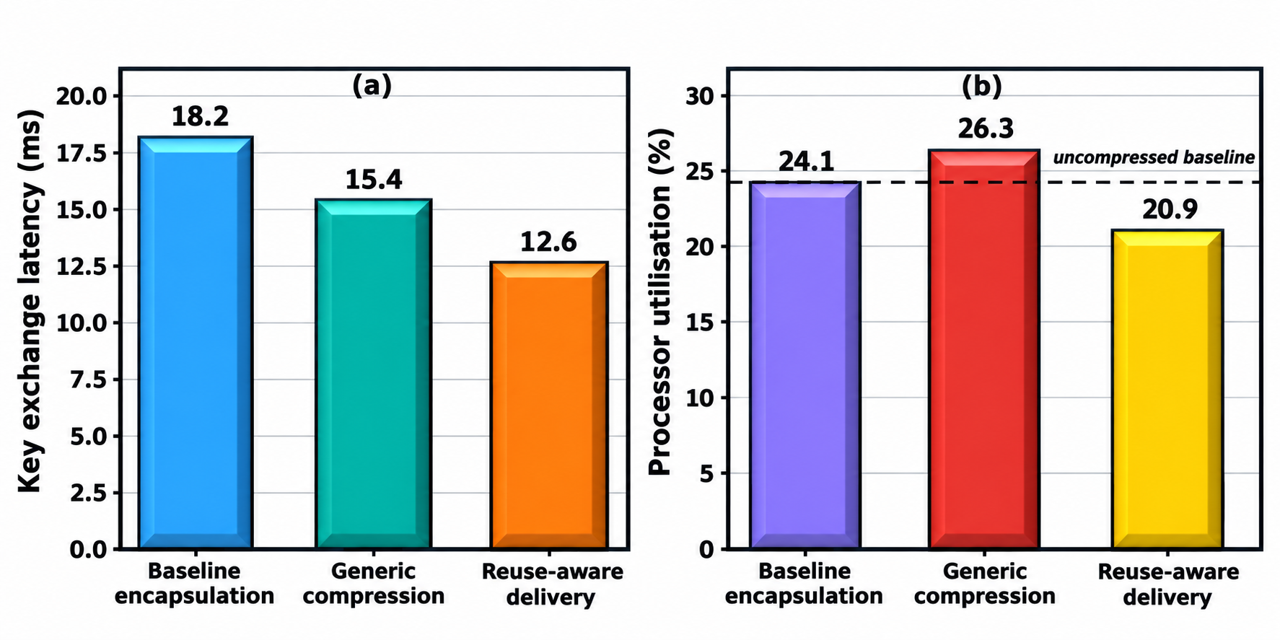
\includegraphics[width=\textwidth]{figures/Picture32.png}
  \caption{Key exchange latency (a) and processor utilisation (b) under three delivery schemes, with the uncompressed baseline marked.}
  \label{fig:pq-latency}
\end{figure}

Generic compression buys latency by spending processor time, reducing the exchange from 18.2 to 15.4~ms while raising utilisation from 24.1\% to 26.3\%, above the uncompressed baseline marked on the second panel. On a device whose primary duty is measurement and actuation that is the wrong trade, and it is the trade a deployment would unknowingly accept by applying a general-purpose compressor to post-quantum traffic. The reuse-aware scheme lowers both, reducing exchange latency by 30.7\% against the uncompressed baseline and by 18.2\% against generic compression while using less processor than either, at 20.9\%. The explanation is structural rather than incidental: fragments that are not retransmitted are also not compressed, decompressed, or reassembled, so avoiding work costs less than compressing it.

The cost of the individual primitives completes the picture, and Figure~\ref{fig:pq-operations} reports them separated by how often the architecture invokes each.
\begin{figure}[!htbp]
  \centering
  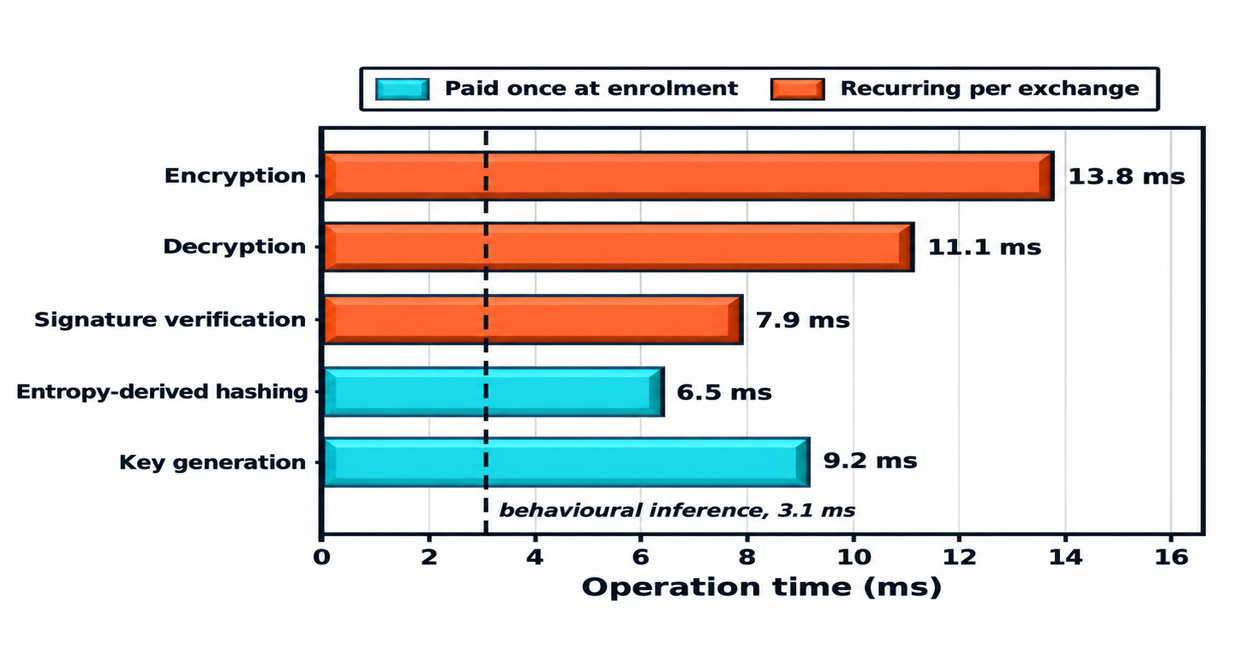
\includegraphics[width=\textwidth]{figures/Picture33.png}
  \caption{Measured cost of quantum-resilient operations on edge-class hardware, separated by enrolment and recurring use, against the behavioural inference time.}
  \label{fig:pq-operations}
\end{figure}
Enrolment operations are paid once and are irrelevant to steady-state cost, so the 9.2 and 6.5~ms attaching to key generation and hashing bear on commissioning rather than on operation. The operations that recur are encryption and decryption at 13.8 and 11.1~ms and signature verification at 7.9~ms, which together place a per-exchange cryptographic cost of 32.8~ms. Set against the 3.1~ms of behavioural inference reported earlier and marked on the figure, cryptography rather than detection is the dominant per-operation cost at the edge by a factor of roughly ten. That ordering is worth stating plainly, since it directs any future effort at reducing edge overhead toward the cryptographic path rather than toward further trimming a detector already at 41{,}762 parameters.

Selection of the primitive family followed from the same constraint rather than from a security ranking. Code-based constructions offer strong security with public keys too large for embedded nodes. Multivariate schemes have been weakened by structural attacks. Hash-based signatures are robust but impose signature sizes a low-rate link cannot absorb. The leading isogeny-based candidate, SIKE, has been broken by a classical key-recovery attack. Lattice constructions were adopted because they combine compact key material with speed adequate for constrained deployment, which is a suitability argument and is presented as one.

Two constraints bound the scope of these measurements. The compression and latency figures were obtained on a workstation-class bench, with microbenchmarks on a single-board computer, and therefore characterise the primitives rather than the microcontroller-class parts at the lower end of the device spectrum, on which the same operations would be slower in proportion to clock. Separately, the ledger bridge binding revocation to the anchoring stratum was specified but not implemented in the identity work, so the evidence reported here covers derivation, delivery, and decoding alone. The anchoring path on which those credentials depend is evidenced separately on the two ledger instantiations, and it is the binding of the two that the architecture contributes rather than either in isolation.
Post-quantum identity is therefore affordable on the hardware the architecture targets. Close to half of the ciphertext is suppressed under reuse-aware delivery, 410 of 768 bytes being sent, because the receiver already holds most of it; the exchange completes in 12.6~ms at lower processor cost than either alternative, and derivation supplies an identifier that is unenumerable when published and bound to behaviour when evaluated.


\subsection{Responsive Trust Decay and Credential Isolation}
\label{sec:eval-isolation}

Detection, commitment, and credential issue are preparatory. What the architecture ultimately does with them is withdraw a device that has begun to misbehave, and that is the operation on which its security claim finally rests. Two properties decide whether withdrawal is dependable. It must be driven by accumulated evidence rather than by a single observation, since a mechanism reacting to one detection would withdraw healthy devices on transient noise and a mechanism ignoring sustained degradation would retain compromised ones. And it must complete quickly enough that the interval during which a device known to be misbehaving still holds an honoured credential is short. The first is a property of the decay law, the second of the path between the flag and the ledger, and both are examined here together with what detection does while isolation is under way.
 
Withdrawal is governed by a trust score that falls on anomalous behaviour and recovers on normal behaviour, with two independent triggers. The score is decremented by the anomaly penalty and credited by the normal increment at each behaviour cycle, and withdrawal follows either when the score falls to the revocation threshold or when consecutive anomalous cycles exceed the streak limit. Figure~\ref{fig:iso-decay} shows the resulting trajectories for a device behaving normally and a device under sustained compromise.

\begin{figure}[!htbp]
  \centering
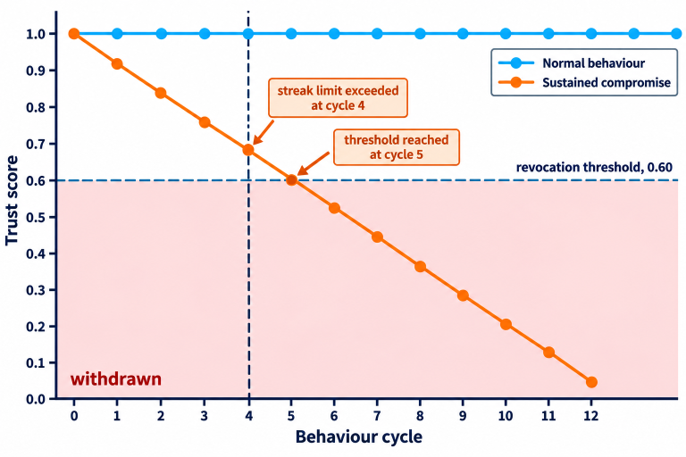
\includegraphics[width=0.98\textwidth]{figures/Picture35.png}
  \caption{Trust score evolution across behaviour cycles for a device behaving normally and a device under sustained compromise, with the revocation threshold and the withdrawn region marked.}
  \label{fig:iso-decay}
\end{figure}

The decline under sustained compromise is linear rather than exponential, which follows directly from the additive form of the law and has a consequence worth drawing out. Each anomalous cycle costs a fixed 0.08 of score, the difference between the anomaly penalty and the normal increment, so a device starting at full trust reaches the threshold of 0.60 at the fifth cycle. The number of cycles to withdrawal is therefore computable in advance from the starting score, the threshold, and the penalty, and an operator may choose the penalty to meet a required response time rather than tuning it by observation. The normal trajectory holds at its ceiling over the same interval, so a device supplying clean evidence accumulates credit rather than drifting downward, and the separation between the two widens by a fixed amount every cycle rather than depending on a single decision point.
 
The streak trigger addresses the case the threshold handles poorly, and the figure shows it firing first. A device compromised abruptly and comprehensively would, under the threshold alone, take as many cycles to withdraw as one degrading slowly, since the score falls at the same rate in both cases. Counting consecutive anomalous cycles short-circuits that delay: with a streak limit of three, a device failing every cycle in succession is withdrawn at the fourth cycle, one cycle before its score would have reached the threshold. The saving is a single cycle in this configuration and grows as the starting score rises or the penalty falls, so the two triggers answer different adversaries, gradual degradation and abrupt compromise, and the streak trigger bounds the delay that the threshold alone would leave open.
 
Elapsed time from the decision to withdraw to its confirmation on the ledger determines how long the credential remains honoured after the finding. Table~\ref{tab:iso-latency} reports that interval together with the detection quality sustained during the same runs.

\begin{table}[!htbp]
  \centering
  \footnotesize
  \setlength{\tabcolsep}{5pt}
  \renewcommand{\arraystretch}{1.3}
  \caption{Revocation latency and the detection quality sustained during isolation.}
  \label{tab:iso-latency}
  \begin{tabularx}{\textwidth}{@{}
      >{\raggedright\arraybackslash}p{5.4cm}
      >{\raggedright\arraybackslash}p{3.0cm}
      >{\raggedright\arraybackslash}X@{}}
    \toprule
    \textbf{Quantity} & \textbf{Measured} & \textbf{Basis} \\
    \midrule
    Revocation latency, flag to ledger confirmation & 1.8 $\pm$ 0.2~s & Mean over five trials \\
    Chaincode updates per revocation & Two signed updates & Per revocation event \\
    Cross-chain confirmations per revocation & One relay confirmation & Per revocation event \\
    Detection accuracy during isolation runs & 97.40\% & Same runs \\
    False positive rate & 1.90\% & Same runs \\
    False negative rate & 0.70\% & Same runs \\
    \bottomrule
  \end{tabularx}
\end{table}

Confirmation completes in 1.8~s with a spread of 0.2~s across trials, and each revocation requires two signed chaincode updates and one cross-chain relay confirmation. The narrowness of that spread matters as much as its magnitude, since a withdrawal path whose latency varied widely would leave the exposure interval unpredictable even where its mean was acceptable. The 1.8~s is measured to confirmation of the updated device status on the permissioned ledger, which is the point at which consortium participants stop honouring the credential. Publication to relying parties outside the consortium follows asynchronously through the relay, at 2.1~s between substrates under stable conditions (Table~\ref{tab:trilemma-close}), together with the confirmation depth of the public chain. The 1.8~s is also not directly comparable with the 0.11~s finalisation reported earlier, since the two were measured on different instantiations; the larger figure reflects the two signed chaincode updates each withdrawal requires on the Fabric realisation rather than a cost of the withdrawal path as such.
 
Detection quality during those runs is unchanged from the figures reported for the behavioural stratum, at 97.40\% accuracy with a false positive rate of 1.90\% and a false negative rate of 0.70\%. That invariance is the second half of what this subsection must establish, since a mechanism that isolated reliably while degrading detection would have traded one capability for another. The false positive rate bounds the cost of the mechanism in the other direction: it is the proportion of clean behaviour misread as evidence, and under an additive law those misreadings are absorbed by the normal increment across subsequent cycles rather than accumulating, so isolated false positives do not drive a healthy device toward the threshold. 
Reliability of the mechanism under load is reported in Figure~\ref{fig:iso-scale}, which gives the proportion of detected anomalies resulting in a completed withdrawal across device populations and placement strategies.

\begin{figure}[!htbp]
  \centering
  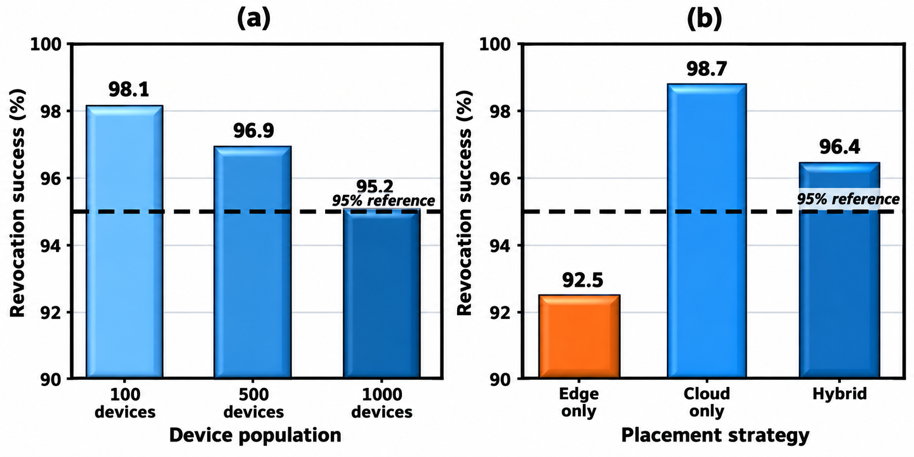
\includegraphics[width=\textwidth]{figures/Picture36.png}
  \caption{Proportion of detected anomalies resulting in a completed withdrawal, across device populations (a) and placement strategies (b).}
  \label{fig:iso-scale}
\end{figure}

Withdrawal succeeds for 98.1\% of detected anomalies at a hundred devices, 96.9\% at five hundred, and 95.2\% at a thousand. A tenfold increase in population therefore costs 2.9 percentage points of success, which is a gentle decline rather than a collapse, and it is the shape the partition predicts: the permissioned layer absorbs the growth in behavioural traffic while the withdrawal path itself is governed by the rate at which devices misbehave rather than by how many devices are present. Success remaining above 95\% at the largest population is the property that matters operationally, since a mechanism degrading sharply with scale would fail precisely in the deployments where isolation is most needed.

Placement tells a different story and exposes the one configuration that underperforms. Cloud placement achieves 98.7\% and hybrid placement 96.4\%, while edge-only placement falls to 92.5\%, below the level sustained by every permissioned configuration in the first panel. The explanation is consistent with the resource evidence presented earlier: an edge-only arrangement performs both evaluation and the assembly of the withdrawal record on the constrained device, and the same budgets that make behavioural scoring affordable there leave little headroom for the additional signing and relay work a withdrawal requires. Hybrid placement, which keeps evaluation at the edge and moves finalisation off it, recovers most of that margin at a cost of 2.3 percentage points against cloud placement, and it is the arrangement the architecture adopts.

Decay-based withdrawal therefore isolates a misbehaving device dependably and without cost to detection. The decline under sustained compromise is linear and its duration computable in advance, two triggers cover gradual and abrupt compromise respectively, confirmation reaches the ledger in 1.8~s with a spread of 0.2~s, success remains above 95\% across a tenfold increase in device population, and accuracy, false positive rate, and false negative rate are unchanged from those reported for the behavioural stratum operating without isolation under way.


\subsection{Substrate-Independent Realisation of the Partition}
\label{sec:eval-substrate}
The generality of a trust-partitioning design is a function of whether the roles it assigns can be discharged by unrelated machinery. The values in Table~\ref{tab:sub-mapping} summarise the component discharging each architectural role in the two realisations of the partition.
\begin{table}[!htbp]
  \centering
  \footnotesize
  \setlength{\tabcolsep}{5pt}
  \renewcommand{\arraystretch}{1.3}
  \caption{Architectural roles and the component discharging each in the two realisations.}
  \label{tab:sub-mapping}
  \begin{tabularx}{\textwidth}{@{}
      >{\raggedright\arraybackslash}p{3.0cm}
      >{\raggedright\arraybackslash}X
      >{\raggedright\arraybackslash}X@{}}
    \toprule
    \textbf{Role} & \textbf{Realisation I} & \textbf{Realisation II} \\
    \midrule
    Behavioural execution
      & Native fast execution layer, one record per observation window
      & Permissioned chaincode invoked per observation window \\
    Ordering and finality
      & Authority-weighted consensus, adaptive cadence, final on commit
      & Ordering service under endorsement policy, final on commit \\
    Validator identity
      & Consortium validators with authority weights and reliability tracking
      & Organisation-scoped identities from a membership service \\
    Public anchoring
      & Companion anchor receiving epoch roots, fee-free
      & General-purpose public chain, contract call, confirmation depth of three \\
    Boundary content
      & Digests and hashed identifiers only
      & Digests and hashed identifiers only \\
    \bottomrule
  \end{tabularx}
\end{table}
The data presented in Table~\ref{tab:sub-mapping} indicate that each architectural role is discharged in both realisations by components that share no consensus mechanism, no execution model, and no cost model. Four of the five rows differ entirely, spanning authority-weighted consensus against an ordering service, adaptive cadence against endorsement policy, weighted consortium validators against organisation-scoped membership identities, and fee-free anchoring against a priced public chain with a confirmation depth of three. The fifth row is identical in both, carrying digests and hashed identifiers and nothing further, which is the invariant by which the partition is defined.

The values in Table~\ref{tab:sub-properties} summarise the properties measured independently on each realisation.
\begin{table}[!htbp]
  \centering
  \footnotesize
  \setlength{\tabcolsep}{5pt}
  \renewcommand{\arraystretch}{1.3}
  \caption{Partition properties measured independently on the two realisations.}
  \label{tab:sub-properties}
  \begin{tabularx}{\textwidth}{@{}
      >{\raggedright\arraybackslash}p{4.0cm}
      >{\raggedright\arraybackslash}X
      >{\raggedright\arraybackslash}X@{}}
    \toprule
    \textbf{Property} & \textbf{Realisation I} & \textbf{Realisation II} \\
    \midrule
    Commitment finality & 0.11~s, final on commit & Final on commit, confirmation depth on the public side only \\
    Detection accuracy & 97.70\% and 96.84\% & 97.40\% \\
    Anchoring cost model & Fee-free throughout & Priced per commitment and per withdrawal \\
    Throughput under load & Sustained across the evaluated workload & 94 tx/s on Fabric with anchoring active, against 80 tx/s Fabric-only (relay experiment); 840 to 940 tx/s under the scaling workload \\
    Withdrawal confirmation & Committed on the permissioned layer & 1.8 $\pm$ 0.2~s to ledger confirmation \\
    Boundary content & Digests only & Digests only \\
    \bottomrule
  \end{tabularx}
\end{table}
The results in Table~\ref{tab:sub-properties} affirm that the properties claimed for the partition hold on both realisations. Commitment is final on commit in each, with confirmation depth arising only where the public substrate requires it. Detection accuracy spans 96.84\% to 97.70\%, a range of 0.86 percentage points across three datasets and two training regimes. Withdrawal reaches ledger confirmation in 1.8~s with a spread of 0.2~s, and the boundary carries digests alone in both cases.

Two results follow from the assignment of roles. Public-chain expenditure on the second realisation splits as the cost relation of Equation~\eqref{eq:anchor-cost} predicts, at 4.20~USD per epoch commitment against 3.50~USD per published withdrawal, assuming a gas price of 20~gwei and an ether price of 3{,}500~USD at May 2025 rates~\cite{amadi2026symmetric}. In the relay experiment, adding the anchoring layer raised Fabric throughput from 80 to 94 transactions per second, an improvement of 17.5\%, since anchoring discharges retention away from the fast layer; the 840 to 940 transactions per second of Table~\ref{tab:sota-robustness} were measured separately under the scaling workload.
The partition is therefore specifiable independently of consensus mechanism, holds under a change from fee-free to priced anchoring, is indifferent to federated or centralised training, and is satisfiable on a production enterprise stack as readily as on a purpose-built lightweight ledger. 

\section{Performance Evaluation with State-of-the-Art Approaches}
\label{sec:eval-sota}
This section evaluates the proposed architecture against recent federated blockchain intrusion detection systems and representative ledger-based data-sharing frameworks. The evaluation covers detection performance, blockchain-level cost and assurance, capability coverage across the security functions each framework provides, and robustness under varying device population and component placement.
 
\subsection{Detection Performance Against Recent Approaches}
\label{sec:sota-detection}
The results in Table~\ref{tab:sota-detection} summarise the detection performance of the proposed architecture and recent federated blockchain intrusion detection approaches, together with the model family and target system of each.
 
\begin{table}[!htbp]
  \centering
  \footnotesize
  \setlength{\tabcolsep}{4pt}
  \renewcommand{\arraystretch}{1.3}
  \caption{Detection performance of the proposed architecture against recent federated blockchain intrusion detection approaches.}
  \label{tab:sota-detection}
  \begin{tabularx}{\textwidth}{@{}
      >{\raggedright\arraybackslash}p{2.0cm}
      >{\raggedright\arraybackslash}p{0.9cm}
      >{\raggedright\arraybackslash}X
      >{\raggedright\arraybackslash}p{2.0cm}
      >{\raggedright\arraybackslash}p{1.5cm}
      >{\raggedright\arraybackslash}p{1.5cm}@{}}
    \toprule
    \textbf{Reference} & \textbf{Year} & \textbf{AI model} & \textbf{Target system} & \textbf{$A_{cc}$ (\%)} & \textbf{$R_c^{+}$ (\%)} \\
    \midrule
    \cite{Anitha2}     & 2024 & Capsule autoencoder & IIoT & 99.97 & 99.88 \\
    \cite{Metaverse}   & 2024 & CNN and MLP & Metaverse & 99.28 & n/r \\
    \cite{bfls}        & 2023 & CNN & General IoT & 98.92 & 98.90 \\
    \cite{FLBC-IDS}    & 2024 & EfficientNet and CNN & General IoT & 98.89 & 98.04 \\
    \cite{enhanced}    & 2024 & Generative adversarial & IIoT & n/r & 98.99 \\
    \cite{vehicula}    & 2021 & MLP & Vehicular IoT & 94.00 & 95.00 \\
    \cite{hbf}         & 2022 & Deep feed forward & General IoT & 90.46 & n/r \\
    \cite{BlockHunter} & 2022 & Clustering ensemble & IIoT & n/r & n/r \\
    \midrule
    Proposed (STRATA) & 2026 & CNN and LSTM & IIoT & 97.70 & 97.70 \\
    \bottomrule
  \end{tabularx}
  \vspace{2pt}
  \parbox{\linewidth}{\footnotesize n/r: not reported by the cited work.}
\end{table}
The data indicate that the proposed architecture achieves an accuracy of 97.70\% and a recall of 97.70\%, which is only slightly lower than the 99.97\% reported by the capsule autoencoder and the 99.28\% reported by the metaverse-targeted approach. The margin against the strongest entry is 2.27 percentage points. That margin is a direct consequence of model size: the capsule autoencoder carries 1.2 million parameters against the 41{,}762 of the proposed module and requires 1.8~MB of memory against 0.17~MB, so the accuracy it attains is available only at a footprint exceeding the budget of a microcontroller-class industrial node. Nevertheless, the proposed architecture exceeds the two remaining approaches that report accuracy, at 94.00\% and 90.46\%, and of the three entries targeting industrial deployment it is one of only two to report accuracy at all. It is also the only entry reporting identical accuracy and recall.
 
Secondly, in terms of balance between the two error types, the proposed architecture returns accuracy and recall at the same value while all four approaches reporting both exhibit some divergence between them, ranging from 0.02 to 1.00 percentage points. Thirdly, in terms of target system, three of the eight approaches address industrial deployment specifically, and of those the proposed architecture is the only one evaluated on industrially generated traffic in addition to a public benchmark.

\subsection{Blockchain-Level Reporting Against the Same Approaches}
\label{sec:sota-blockchain}
The results in Table~\ref{tab:sota-blockchain} highlight the blockchain-level characterisation of the proposed architecture and the same eight approaches, covering network type, transaction cost, contract assurance, and support for constrained nodes.
\begin{table}[!htbp]
  \centering
  \footnotesize
  \setlength{\tabcolsep}{4pt}
  \renewcommand{\arraystretch}{1.3}
  \caption{Blockchain-level characterisation of the proposed architecture against the same approaches.}
  \label{tab:sota-blockchain}
  \begin{tabularx}{\textwidth}{@{}
      >{\raggedright\arraybackslash}p{2.4cm}
      >{\raggedright\arraybackslash}X
      >{\raggedright\arraybackslash}p{2.0cm}
      >{\raggedright\arraybackslash}p{2.0cm}
      >{\raggedright\arraybackslash}p{2.2cm}@{}}
    \toprule
    \textbf{Reference} & \textbf{Network type} & \textbf{Gas cost} & \textbf{Security audit} & \textbf{Lightweight nodes} \\
    \midrule
    \cite{Anitha2}     & Not stated & n/r & n/r & n/r \\
    \cite{Metaverse}   & Public & 63{,}007 & No & No \\
    \cite{bfls}        & n/r & n/r & n/r & n/r \\
    \cite{FLBC-IDS}    & Permissioned & n/r & No & No \\
    \cite{enhanced}    & Permissioned & n/r & n/r & n/r \\
    \cite{vehicula}    & Public & n/r & n/r & n/r \\
    \cite{hbf}         & Permissioned & n/r & n/r & n/r \\
    \cite{BlockHunter} & Public & n/r & n/r & n/r \\
    \midrule
    Proposed (STRATA) & Hybrid & 65{,}618 & 98\% & Yes \\
    \bottomrule
  \end{tabularx}
  \vspace{2pt}
  \parbox{\linewidth}{\footnotesize n/r: not reported by the cited work.}
\end{table}
The proposed architecture consumes 65{,}618 gas for model commitment, which is only slightly higher than the 63{,}007 reported by the single approach that quantifies transaction cost. Nevertheless, that approach is the only one of eight to report any blockchain-level cost at all, none of the eight reports a contract security assessment, and none reports support for constrained nodes. All eight employ a distributed ledger and seven leave its cost unquantified, so the practical viability of those deployments remains undetermined regardless of the detection accuracy reported.
The proposed architecture reports 65{,}618 gas for commitment, a contract assessment of 98\% across six vulnerability classes, and a device profile of 41{,}762 parameters at 0.17~MB with an inference latency of 3.1~ms, and is accordingly the only entry in the comparison characterised across the artificial-intelligence layer, the blockchain layer, and the device budget simultaneously.

\subsection{Discussion of Comparative Performance}
\label{sec:sota-discussion}
Based on the presented comparative analysis, the proposed architecture achieves a detection accuracy of 97.70\% with recall at the same value, a commitment cost of 65{,}618 gas at a finalisation latency of 0.11~s, a contract assessment of 98\%, and a device footprint of 0.17~MB at 3.1~ms per inference. Approaches attaining higher raw accuracy do so with models between fifteen and roughly one hundred times larger. All but one of them exceed the memory available on microcontroller-class industrial nodes, which confines behavioural evaluation to a gateway or a server, and the one that fits at rest, at 0.9~MB, leaves little headroom once activation buffers are allocated.
Jointly optimising the detector and the ledger deployment, and characterising both against the resource constraints of industrial edge hardware, is what distinguishes the proposed architecture from approaches optimising either in isolation. The comparison therefore establishes the proposed architecture as a deployable option for industrial environments in which detection quality, ledger cost, contract assurance, and device budget must be satisfied together rather than individually.


\subsection{Comparison with Related Hybrid-Ledger Approaches}
\label{sec:sota-related}
The results in Table~\ref{tab:sota-related} highlight the capability coverage of the proposed architecture and representative ledger-based data-sharing frameworks across device lifecycle management, threat detection, quantum-resilient cryptography, public auditability, and performance reporting.
\begin{table}[!htbp]
  \centering
  \footnotesize
  \setlength{\tabcolsep}{4pt}
  \renewcommand{\arraystretch}{1.3}
  \caption{Capability coverage of the proposed architecture against representative ledger-based data-sharing frameworks.}
  \label{tab:sota-related}
  \begin{tabularx}{\textwidth}{@{}
      >{\raggedright\arraybackslash}p{2.4cm}
      >{\raggedright\arraybackslash}p{2.1cm}
      >{\centering\arraybackslash}p{0.9cm}
      >{\centering\arraybackslash}p{0.9cm}
      >{\centering\arraybackslash}p{1.2cm}
      >{\centering\arraybackslash}p{1.2cm}
      >{\raggedright\arraybackslash}X@{}}
    \toprule
    \textbf{Method} & \textbf{Chain type} & \textbf{DLM} & \textbf{ITD} & \textbf{PQC} & \textbf{Audit} & \textbf{Performance reporting} \\
    \midrule
    \cite{yangwei}    & Single & \checkmark & $\times$ & $\times$ & \checkmark & Limited, chain focus \\
    \cite{liu}        & Permissioned & \checkmark & \checkmark & $\times$ & $\times$ & Limited, case specific \\
    \cite{reshma}     & Hybrid & \checkmark & $\times$ & $\times$ & \checkmark & Partial, crypto focus \\
    \cite{wang}       & Hybrid & \checkmark & $\times$ & $\times$ & \checkmark & Partial, health domain \\
    \cite{erukala}    & Hybrid & \checkmark & $\times$ & $\times$ & \checkmark & Limited, end-to-end communication \\
    \cite{ghaemi}     & Single with QC & $\times$ & $\times$ & \checkmark & $\times$ & Partial, authentication protocol \\
    \cite{aslam}      & Single with PQC & $\times$ & $\times$ & \checkmark & \checkmark & Partial, consensus and cryptography \\
    \cite{venkatesh}  & Single with QC & $\times$ & $\times$ & \checkmark & $\times$ & Partial, lightweight claims \\
    \midrule
    Proposed (STRATA) & Hybrid & \checkmark & \checkmark & \checkmark & \checkmark & Full, learning, cryptography, ledger and robustness \\
    \bottomrule
  \end{tabularx}
  \vspace{2pt}
  \parbox{\linewidth}{\footnotesize\raggedright
  DLM-device lifecycle management; ITD-intelligent threat detection; PQC-post-quantum and quantum-resilient cryptography.}
\end{table}
It indicates that the architecture is the only entry supporting all four capabilities. Five of the eight frameworks provide device lifecycle management, one provides intelligent threat detection, three provide quantum-resilient cryptography, and five provide public auditability, with no framework supporting more than three of the four.
 
The coverage divides along a consistent line. The five frameworks providing lifecycle management and auditability rely on classical cryptography and address no quantum threat, while the three providing quantum-resilient cryptography operate on single-chain designs and provide neither lifecycle governance nor ledger-triggered revocation. Threat detection appears in one framework alone and is not coupled to revocation in that case. The proposed architecture combines lifecycle governance, hybrid-chain auditability, and learning-driven revocation within a single operational workflow, which is consistent with the latency, throughput, and revocation results reported earlier in this chapter.
Performance reporting separates the entries further. Seven of the eight frameworks report performance partially, confined to a chain, a protocol, or a domain, and one reports it in limited form. The proposed architecture reports detection quality, cryptographic overhead, ledger cost, and robustness across deployment conditions under a single experimental setting, which permits the four to be assessed jointly rather than in isolation.

\subsection{Robustness Across Deployment Conditions}
\label{sec:sota-robustness}
The values in Table~\ref{tab:sota-robustness} summarise latency, throughput, and revocation success across six deployment scenarios spanning device population and component placement.
\begin{table}[!htbp]
  \centering
  \footnotesize
  \setlength{\tabcolsep}{5pt}
  \renewcommand{\arraystretch}{1.3}
  \caption{Latency, throughput, and revocation success across six deployment scenarios, mean of five runs.}
  \label{tab:sota-robustness}
  \begin{tabularx}{\textwidth}{@{}
      >{\raggedright\arraybackslash}p{4.6cm}
      >{\raggedright\arraybackslash}X
      >{\raggedright\arraybackslash}X
      >{\raggedright\arraybackslash}X@{}}
    \toprule
    \textbf{Scenario} & \textbf{Latency (ms)} & \textbf{Throughput (tx/s)} & \textbf{Revocation success (\%)} \\
    \midrule
    100 devices & 32.4 & 910 & 98.1 \\
    500 devices & 47.8 & 885 & 96.9 \\
    1000 devices & 68.3 & 840 & 95.2 \\
    Edge-only placement & 54.2 & 740 & 92.5 \\
    Cloud-only placement & 30.7 & 940 & 98.7 \\
    Hybrid placement & 40.1 & 895 & 96.4 \\
    \bottomrule
  \end{tabularx}
\end{table}
The results affirm that the architecture scales without collapse. A tenfold increase in device population raises latency from 32.4 to 68.3~ms and reduces throughput from 910 to 840 transactions per second, a loss of 7.7\%, while revocation success remains above 95\% throughout. Latency increases gradually rather than sharply, which is consistent with leader-driven log replication under the ordering service as the participating population grows.
 
Across placement strategies, cloud placement achieves the highest throughput at 940 transactions per second and the lowest latency at 30.7~ms, and edge-only placement the lowest throughput at 740 and a revocation success of 92.5\%. Hybrid placement returns 895 transactions per second at 40.1~ms with revocation success of 96.4\%, retaining 95\% of cloud throughput while keeping behavioural evaluation on the devices generating the traffic. Revocation success exceeds 95\% in every scenario apart from edge-only placement, confirming that lifecycle enforcement and anomaly-triggered revocation sustain scale across the evaluated deployment range.

\section{Summary of Results}
\label{sec:eval-summary}

After analysing the results and discussions presented, it is possible to establish trustworthy security for constrained industrial deployments in real time by combining behavioural evidence derived from a lightweight learnable model with the finalisation, anchoring, and credential parameters carried by a partitioned hybrid ledger. Behavioural scoring at 41{,}762 parameters and 0.17~MB supplies detection between 96.84\% and 97.70\% within the compute, memory, and energy budgets of microcontroller-class hardware; authority-weighted finalisation commits that evidence in 0.11~s without confirmation depth; epoch anchoring places a compact proof of it beyond the reach of the operating consortium; and entropy-seeded credentials delivered under post-quantum encapsulation bind each verdict to a device whose identifier cannot be enumerated from the public record.

With the proposed STRATA architecture in place, there is an enhancement in the security capacity of constrained industrial deployments for continuous and verifiable monitoring, since each security function is discharged on the layer whose cost profile sustains it rather than uniformly across devices that cannot afford uniform protection. High-frequency behavioural validation is absorbed by a fast permissioned layer at 0.13\% of the link the learning traffic already occupies, while low-frequency identity anchoring, audit, and revocation are committed to a separate public layer at a cost governed by how often devices misbehave rather than by how much traffic they generate. Credential withdrawal follows accumulated evidence rather than a single detection, reaching ledger confirmation in 1.8~s and succeeding for above 95\% of detected anomalies across a tenfold increase in device population, without degradation of the detection quality on which those decisions rest.

This combined approach ensures that an industrial deployment is capable of detecting anomalous device behaviour, attributing it to an identified credential, and withdrawing that credential verifiably, while continuing to monitor throughout. Detection persists during consensus outage because behavioural scoring is placed below the consensus layer, so a validator failure costs freshness of the global model rather than coverage of the plant. Anchoring imposes no disclosure surface, since digests and hashed identifiers alone cross the trust boundary on both realisations. Contract assurance across six vulnerability classes returned no critical or high-severity finding, and the architecture is the only entry in the comparative evaluation reporting ledger cost, contract assessment, and support for constrained nodes together.

By realising this approach on two ledger substrates sharing no consensus mechanism, no execution model, and no cost model, the generality of trust-partitioning is established beyond a single implementation. Security functions are placed by cost profile rather than by uniform application, the resulting design operates within the resource limits of industrial edge hardware, and its organising principle transfers to substrates chosen for their difference.

\subsection{Answers to the Research Questions}
\label{sec:eval-rq}

Table~\ref{tab:rq-answers} draws the results of this chapter together against the five research questions posed in Section~\ref{sec:rq}, stating for each the principal evidence, the section in which it is reported, and the extent to which the question is answered. Where an answer holds only within a stated scope, the scope is recorded rather than left implicit.

\begin{table}[!htbp]
  \centering
  \footnotesize
  \setlength{\tabcolsep}{4pt}
  \renewcommand{\arraystretch}{1.3}
  \caption{Answers to the research questions, with the principal evidence and its location in this chapter.}
  \label{tab:rq-answers}
  \begin{tabularx}{\textwidth}{@{}
      >{\raggedright\arraybackslash}p{0.9cm}
      >{\raggedright\arraybackslash}X
      >{\raggedright\arraybackslash}p{2.0cm}
      >{\raggedright\arraybackslash}p{3.0cm}@{}}
    \toprule
    \textbf{RQ} & \textbf{Principal evidence} & \textbf{Reported in} & \textbf{Answer} \\
    \midrule
    RQ1 & Permissioned finalisation in 0.11~s with no confirmation depth; ledger metadata at 0.13\% of the learning uplink; public-layer cost governed by the revocation rate rather than traffic volume; anchoring raises Fabric throughput from 80 to 94~tx/s
        & Sections~\ref{sec:eval-resource}, \ref{sec:eval-ledger}, \ref{sec:eval-substrate}
        & Yes: partitioning delivers verifiable security within device and ledger budgets \\
    RQ2 & 41{,}762 parameters at 0.17~MB (peak below 0.6~MB), 3.1~ms inference, 6 to 9\% processor occupancy; accuracy 96.84 to 97.70\% across three datasets; federation costs at most 0.003 in F1
        & Sections~\ref{sec:eval-evidence} to~\ref{sec:eval-resource}
        & Yes, on edge-class hardware; energy figure estimated rather than instrumented \\
    RQ3 & Kyber512 ciphertext reduced from 768 to 410~bytes (46.6\%); key exchange 30.7\% faster at lower processor load; identifiers of 128 bits and above
        & Section~\ref{sec:eval-identity}
        & Yes, on a workstation bench with single-board microbenchmarks; ledger bridge specified but not implemented \\
    RQ4 & The same partition realised on PureChain NSL and on Fabric with Ethereum, sharing no consensus, execution, or cost model; boundary content limited to digests in both
        & Section~\ref{sec:eval-substrate}
        & Yes, on two substrate pairs; a general characterisation remains open \\
    RQ5 & Two independent withdrawal triggers; confirmation in 1.8~$\pm$~0.2~s; success of 95.2\% or more up to 1{,}000 devices; detection unchanged during isolation (97.40\%, false positive rate 1.90\%); contract assessment of 98\%
        & Sections~\ref{sec:eval-security}, \ref{sec:eval-isolation}, \ref{sec:sota-robustness}
        & Yes, within the evaluated threat model; inference attacks on model updates not mitigated \\
    \bottomrule
  \end{tabularx}
\end{table}

\subsection{Resolution of the Security, Scalability, and Speed Trilemma}
\label{sec:eval-trilemma}
The security, scalability, and speed trilemma presented at the outset of this thesis holds within a single distributed ledger, where optimising any two dimensions is obtained at the expense of the third. The values in Table~\ref{tab:trilemma-close} summarise the evidence obtained on each dimension and the layer supplying it.

\begin{table}[!htbp]
  \centering
  \footnotesize
  \setlength{\tabcolsep}{5pt}
  \renewcommand{\arraystretch}{1.3}
  \caption{Evidence obtained on each dimension of the trilemma and the layer supplying it.}
  \label{tab:trilemma-close}
  \begin{tabularx}{\textwidth}{@{}
      >{\raggedright\arraybackslash}p{2.0cm}
      >{\raggedright\arraybackslash}p{3.2cm}
      >{\raggedright\arraybackslash}X
      >{\raggedright\arraybackslash}p{2.4cm}@{}}
    \toprule
    \textbf{Dimension} & \textbf{Supplied by} & \textbf{Measured evidence} & \textbf{Cost incurred} \\
    \midrule
    Security
      & Public anchoring stratum, with contract assessment on the permissioned layer
      & No critical or high-severity finding across six vulnerability classes at an overall assessment of 98\%; integrity preserved beyond the fault bound, with unvalidated updates unable to reach the immutable layer
      & Anchoring fee per epoch and per withdrawal \\
    Speed
      & Consensus and coordination stratum
      & Finalisation in 0.11~s with no confirmation depth; behavioural inference in 3.1~ms at the edge; withdrawal confirmed in 1.8~s
      & Validator set restricted to identified participants \\
    Scalability
      & Separation of the two strata
      & Throughput of 840 to 910 transactions per second across 100 to 1000 devices, and up to 940 under cloud placement, a reduction of 7.7\% across a tenfold population increase under the scaling workload; in the relay experiment, 94 against 80 transactions per second relative to a Fabric-only baseline
      & Relay latency of 2.1~s between substrates under stable conditions \\
    \bottomrule
  \end{tabularx}
\end{table}

The data presented indicate that each dimension is discharged by a different part of the architecture and paid for in a currency the supplying layer sustains. Security rests on a substrate outside consortium administration, which incurs a transaction fee and no latency penalty, since anchoring proceeds asynchronously to the control loop it protects. Speed rests on assigned rather than contested authority, which restricts participation and returns deterministic finality at a tenth of a second. Scalability arises from the separation itself rather than from optimisation within either layer, as evidenced by the single-chain comparison in which the addition of the anchoring layer raised throughput by 17.5\% rather than lowering it.

The trilemma is therefore not resolved within a layer but dissolved across two. Once each demand is routed to the layer whose cost profile matches it, the trade-offs that bind within a single ledger become budgetary decisions distributed between substrates, and the architecture sustains all three dimensions simultaneously at the operating points reported throughout this chapter. Trust-partitioning accordingly delivers lightweight, verifiable, and quantum-resilient security for constrained mission-critical industrial deployments, which is the position the thesis set out to establish.

\chapter{Conclusion, Practical Concerns and Future Works}
% \pagenumbering{arabic}
\Large
\label{Chapter_6}
\section{Conclusion}
\label{sec:conclusion}

This thesis proposed a trust-partitioning architecture that delivers trustworthy security for constrained, mission-critical industrial deployments by placing each security function on the layer whose cost profile sustains it rather than applying uniform protection across devices that cannot afford it. To establish the proposition, the study developed: (i) STRATA, a unified architecture separating high-frequency behavioural validation on a fast permissioned layer from low-frequency identity anchoring, audit, and revocation committed to a public layer; (ii) a lightweight federated behavioural-trust module built on a trimmed one-dimensional convolutional recurrent model coupled with a resource-optimised permissioned ledger; (iii) a quantum-resilient identity and credential module based on entropy-seeded derivation and compressed post-quantum key delivery; and (iv) a consolidated evaluation spanning detection quality, resource overhead, ledger cost, and quantum resilience across two distinct ledger substrates.

The architecture operates as follows. Behavioural evidence is produced at the edge by a model carrying 41{,}762 parameters at 0.17~MB, committed to the permissioned layer under authority-weighted consensus, aggregated by epoch, and anchored as a digest on a public substrate beyond the reach of the operating consortium. Device credentials are derived from entropy captured at the device and delivered under lattice-based encapsulation, and a trust score accumulated from behavioural evidence drives withdrawal of those credentials through two independent triggers, with the withdrawal published for relying parties who do not trust the operator.

The proposed architecture was evaluated against eight recent federated blockchain approaches and eight representative ledger-based data-sharing frameworks. The results demonstrate that the approach is both adequate and deployable, achieving detection accuracy between 96.84\% and 97.70\% with a false positive rate of 1.90\%, finalisation in 0.11~s without confirmation depth, ledger metadata occupying 0.13\% of the link the learning traffic already uses, a ciphertext reduction of 46.6\% under reuse-aware delivery, and revocation confirmed in 1.8~s with success above 95\% across a tenfold increase in device population. Detection accuracy is 2.27 percentage points below the strongest reported comparator, which attains that result with a model twenty-nine times larger and a memory footprint exceeding the budget of a microcontroller-class industrial node. The architecture is nonetheless the only entry in the comparison reporting ledger cost, contract assessment, and support for constrained nodes together, and the only framework providing device lifecycle management, intelligent threat detection, quantum-resilient cryptography, and public auditability simultaneously.

Each of the five research questions posed in Chapter~\ref{Chapter_1} is answered by this evidence, as Table~\ref{tab:rq-answers} records in full. Trust can be partitioned across a hybrid ledger within real device budgets (RQ1), since finalisation completes in 0.11~s while the ledger occupies 0.13\% of the uplink and public cost is governed by the rate of withdrawal rather than by traffic volume. Lightweight behavioural trust scoring operates inside the budget of edge-class hardware without sacrificing detection (RQ2), at 0.17~MB and 3.1~ms per inference with accuracy between 96.84\% and 97.70\%. Post-quantum identity and credential delivery is affordable on constrained links (RQ3), with the delivered ciphertext reduced from 768 to 410~bytes and the exchange shortened by 30.7\%. The partition holds on two substrate pairs that share no consensus, execution, or cost model (RQ4). Decay-based withdrawal isolates a misbehaving node within 1.8~s, succeeds for more than 95\% of detected anomalies across a tenfold increase in device population, and leaves detection quality unchanged (RQ5). Each answer holds within the scope stated beside it, and the measurements that would extend that scope are identified among the practical concerns that follow.

The experimental results further establish that trust-partitioning is a property of the design rather than of any particular ledger. Each architectural role was discharged on two substrate pairs sharing no consensus mechanism, no execution model, and no cost model, while the boundary carried digests and hashed identifiers alone in each case, and the cost relation derived at design time was exhibited by the measured public-chain prices on the realisation where commitments are priced. The security, scalability, and speed trilemma, which binds within a single distributed ledger, is accordingly dissolved across two, with each demand routed to the layer whose cost profile matches it.

\section{Practical Concerns and Future Works}
\label{sec:future-work}

Deploying a trust-partitioned security architecture on constrained industrial hardware raises several research and implementation concerns that warrant consideration for the wider viability of the approach.

\begin{enumerate}
\item \textbf{Entropy Sourcing on Fielded Hardware.} Identifier derivation consumes a sample from the device entropy source and treats it as an opaque bit string, so the construction is indifferent to which source supplies it. The present realisation is seeded from a software generator, and while the derivation, storage, and lifecycle operations behave as specified under that substitution, the unpredictability a fielded device would obtain remains to be characterised. Hardware sources differ substantially in availability across the industrial device population, from secure elements carrying a dedicated generator to legacy field devices offering only a sensor noise floor. Research establishing the entropy actually attainable on each class of device, together with conditioning procedures appropriate to the weaker sources, would place the unpredictability argument on measured rather than architectural ground.

\item \textbf{Cost of Signature Migration.} Key establishment has been migrated to lattice-based encapsulation, where the exposure is retroactive and migration cannot be deferred. Digital signatures carry a prospective exposure instead, since a signature cannot be forged retrospectively onto a commitment already published, which makes deferral defensible but not indefinite. Migration multiplies key and signature sizes at every point where a block is signed and every point where a credential is presented, and those artefacts are stored rather than transmitted once. Sizing that cost against the storage budget of a field gateway, and identifying which signature family fits it, is an engineering question the present design leaves open.

\item \textbf{Privacy of Model Updates Under Inference Attack.} The federated arrangement preserves data locality by ensuring that raw industrial traffic never leaves the device. Model updates are nonetheless exchanged without secure aggregation or noise injection, a choice made to preserve deployability on nodes whose budgets the evaluation showed to be tight. Within the evaluated threat model the exposure is bounded by authenticated participation, update validation, and ledger-recorded provenance, so inference would have to be attempted from an attributable position. Deployments operating under stronger adversarial privacy requirements would require secure aggregation or differential privacy, and establishing the accuracy and computation cost those mechanisms impose at the parameter counts involved is a direct extension of this work.

\item \textbf{Anchoring Economics Under Congestion.} Public anchoring cost separates into a term compressible by raising the epoch span and a term set by the rate at which devices are withdrawn. That separation was confirmed against measured prices under ordinary conditions, and it establishes that expenditure is governed by how often devices misbehave rather than by how much traffic they generate. Sustained congestion on the public substrate raises the per-commitment fee for both terms simultaneously, and the epoch span can absorb the first but not the second. Research into batching strategies for withdrawal publication, and into anchoring on cost-optimised layers, would extend the economic argument to conditions the present evaluation did not exercise.

\item \textbf{Characterisation of Admissible Substrates.} Realising the partition on two unrelated substrate pairs establishes that the design can be moved, and the properties claimed for it were obtained by machinery with nothing in common. Establishing that it can be moved to any substrate is a stronger claim requiring a characterisation of the substrate properties on which faithfulness depends, together with a proof that any substrate possessing them admits a faithful realisation. That direction also admits a negative formulation, namely whether classes of substrate exist on which no faithful realisation is possible, which would bound the generality of trust-partitioning from below as the two realisations bound it from above. Both formulations are open.

\item \textbf{Industrial Traffic Capture and Dataset Realism.} Evaluation drew on a public network benchmark, a general intrusion benchmark, and an internally generated industrial set constructed at the feature dimensionality the deployed model consumes, with agreement across the three establishing that detection does not depend on the peculiarities of any one. Synthetic generation reproduces the shape of industrial traffic and cannot reproduce the incidents, misconfigurations, and long-tailed device behaviour a live capture would contain. The architecture treats the detector as replaceable for this reason, since behavioural scoring is a stratum with a defined output and a deployment holding proprietary traffic substitutes its own model without disturbing the strata above it. Access to captured operational traffic, and evaluation of the partition under it, would close the remaining distance between benchmark performance and plant performance.

\item \textbf{Instrumented Measurement on Microcontroller-Class Hardware.} Inference latency and processor occupancy were measured on an ARM Cortex-A class environment, the post-quantum delivery figures were obtained on a workstation bench with single-board microbenchmarks, and energy per inference was estimated from an embedded-power model rather than read from an instrumented supply. The memory figures that decide feasibility follow from parameter count and encoding and would carry over unchanged, but latency, occupancy, and energy on a microcontroller with a lower clock and no floating-point unit would not. Repeating the behavioural and cryptographic measurements on instrumented microcontroller-class parts, and implementing the ledger bridge that binds revocation to the anchoring stratum in the identity realisation, would replace the remaining estimates with measurements at the lower end of the device spectrum the architecture targets.
\end{enumerate}



\clearpage
\phantomsection
\large
\addcontentsline{toc}{chapter}{References}
\bibliography{biblio.bib}
\bibliographystyle{ieeetr}

\end{document}
